%-----------------------------------------
% Note: Use pdflatex to process this file.
%
% IMPORTANT: This file uses .aux files from the Bmad manual so pdflatex the Bmad manual beforehand.
%            Note: It is assumed that the bmad and tao directories have the same parent directory.
%-----------------------------------------

\documentclass{book}
\usepackage{xr}       % Defines \externaldocument
\usepackage{graphicx}
\usepackage{moreverb}
\usepackage{amsmath}
\usepackage{alltt}
\usepackage{rotating}
\usepackage{subcaption}
\usepackage{xspace}
\usepackage{makeidx}
\usepackage{multirow}
\usepackage{booktabs}   % For table layouts
\usepackage{longtable}
\usepackage{enumitem} % enumeration lists

\usepackage[T1]{fontenc}   % so _, <, and > print correctly in text.
\usepackage[strings]{underscore}    % to use "_" in text
\usepackage{textcomp}
\usepackage[pdftex,colorlinks=true,bookmarksnumbered=true]{hyperref}  % This must be the last package

\newcommand{\extref}[1]{$\S$\ref*{#1}}   % No hyperlink. For external refs. \extref
\newcommand{\comma}{\> ,}
\newcommand{\period}{\> .}
\newcommand{\wt}{\widetilde}
\newcommand{\grv}{\textasciigrave}
\newcommand{\hyperbf}[1]{\textbf{\hyperpage{#1}}}
\newcommand{\Ss}{\(^*\)}
\newcommand{\Dd}{\(^\dagger\)}

\newcommand{\AND}{&& \hskip -17pt\relax}
\newcommand{\CR}{\\}
\newcommand{\CRNO}{\nonumber \\}
\newcommand{\dstyle}{\displaystyle}

\newcommand{\Begineq}{\begin{equation}}
\newcommand{\Endeq}{\end{equation}}
\newcommand{\NoPrint}[1]{}

\newcommand{\pow}[1]{\cdot 10^{#1}}
\newcommand{\Bf}[1]{{\bf #1}}
\newcommand{\bfr}{\Bf r}

\newcommand{\bmad}{{\sl Bmad}\xspace}
\newcommand{\tao}{{\sl Tao}\xspace}
\newcommand{\mad}{{\sl MAD}\xspace}
\newcommand{\cesr}{{\sl CESR}\xspace}

\newcommand{\sref}[1]{\S\ref{#1}}
\newcommand{\Sref}[1]{Sec.~\sref{#1}}
\newcommand{\cref}[1]{Chapter~\ref{#1}}

\newcommand{\Newline}{\hfil \\ \relax}

\newcommand{\eq}[1]{{(\protect\ref{#1})}}
\newcommand{\Eq}[1]{{Eq.~(\protect\ref{#1})}}
\newcommand{\Eqs}[1]{{Eqs.~(\protect\ref{#1})}}

\newcommand{\vn}{\ttcmd}           % For variable names
\newcommand{\vni}{\ttcmdindx}
\newcommand{\cs}{\ttcmd}           % For code source
\newcommand{\cmd}{\ttcmd}          % For Unix commands
\newcommand{\rn}{\ttcmd}           % For Routine names
\newcommand{\tn}{\ttcmd}           % For Type (structure) names
\newcommand{\bn}[1]{{\bf #1}}       
\newcommand{\toffset}{\vskip 0.01in}
\newcommand{\rot}[1]{\begin{rotate}{-45}#1\end{rotate}}

\newcommand{\data}{{\mbox{data}}}
\newcommand{\reference}{{\mbox{ref}}}
\newcommand{\model}{{\mbox{model}}}
\newcommand{\base}{{\mbox{base}}}
\newcommand{\design}{{\mbox{design}}}
\newcommand{\meas}{{\mbox{meas}}}
\newcommand{\var}{{\mbox{var}}}

\newcommand\ttcmd{\begingroup\catcode`\_=11 \catcode`\%=11 \dottcmd}
\newcommand\dottcmd[1]{\texttt{#1}\endgroup}

\newcommand\ttcmdindx{\begingroup\catcode`\_=11 \catcode`\%=11 \dottcmdindx}
\newcommand\dottcmdindx[1]{\texttt{#1}\endgroup\index{#1}}

\newcommand{\St}{$^{st}$\xspace}
\newcommand{\Nd}{$^{nd}$\xspace}
\newcommand{\Th}{$^{th}$\xspace}
\newcommand{\B}{$\backslash$}
\newcommand{\W}{$^\wedge$}

\newcommand{\cbar}[1]{\overline C_{#1}}

\newlength{\dPar}
\setlength{\dPar}{1.5ex}

\newenvironment{example}
  {\vspace{-3.0ex} \begin{alltt}}
  {\end{alltt} \vspace{-2.5ex}}

\newcommand\Strut{\rule[-2ex]{0mm}{6ex}}

\newenvironment{Itemize}
  {\begin{list}{$\bullet$}
    {\addtolength{\topsep}{-1.5ex} 
     \addtolength{\itemsep}{-1ex}
    }
  }
  {\end{list} \vspace*{1ex}}

\newcommand{\Section}[1]{\section{#1}\indent\vspace{-3ex}}

\newcommand{\SECTION}[1]{\section*{#1}\indent\vspace{-3ex}}

% From pg 64 of The LaTex Companion.

\newenvironment{ventry}[1]
  {\begin{list}{}
    {\renewcommand{\makelabel}[1]{\textsf{##1}\hfil}
     \settowidth{\labelwidth}{\textsf{#1}}
     \addtolength{\itemsep}{-1.5ex}
     \addtolength{\topsep}{-1.0ex} 
     \setlength{\leftmargin}{5em}
    }
  }
  {\end{list}}


\externaldocument[B-]{../../bmad/doc/lattice-file}

\setlength{\textwidth}{6.25in}
\setlength{\oddsidemargin}{0.25in}
\setlength{\evensidemargin}{0.00in}
\setlength{\textheight}{8.5in}
\setlength{\topmargin}{0in}
\setlength{\skip\footins}{6pt}
\setlength{\footnotesep}{3ex}

\setlist[description]{itemsep = 0pt}

\renewcommand{\textfraction}{0.1}
\renewcommand{\topfraction}{1.0}
\renewcommand{\bottomfraction}{1.0}

%%% Table of Contents spacing.
\makeatletter
\renewcommand{\l@section}{\@dottedtocline{1}{1.5em}{3.3em}}
\renewcommand{\l@subsection}{\@dottedtocline{2}{3.8em}{4.2em}}
\renewcommand{\l@figure}{\@dottedtocline{1}{1.5em}{3.3em}}
\renewcommand{\l@table}{\@dottedtocline{1}{1.5em}{3.3em}}
\makeatother

%----------------------------------------------------------------
\makeindex

\begin{document}

\index{lattice!model|see{model lattice}}
\index{lattice!design|see{design lattice}}
\index{lattice!base|see{base lattice}}

\thispagestyle{empty}

\begin{flushright}
\large
Revision: July 16, 2021 \\
\end{flushright}

\vfill

{
\begin{center}
\resizebox{1.8cm}{!}{\Huge \sf\bf The} \\
\vskip 0.2in

\includegraphics[width=10cm]{tao-logo.pdf} \\
\vskip 0.3in
\resizebox{4.4cm}{!}{\Huge \sf\bf Manual} \\
\vskip 0.4in
{\huge \sf\bf David Sagan} \\
\end{center}
}

\vfill
\break


%----------------------------------------------------------------
{
\setlength{\parskip}{\dPar}
\setlength{\parindent}{0ex}
}

%----------------------------------------------------------------

\cleardoublepage
\phantomsection 
\pdfbookmark[0]{Contents}{Contents}
\pdfbookmark[1]{Table of Contents}{toc} 
\tableofcontents


\cleardoublepage
\phantomsection 
\pdfbookmark[1]{List of Figures}{LoF} 
\listoffigures


\cleardoublepage
\phantomsection 
\pdfbookmark[1]{List of Tables}{LoT} 
\listoftables

%----------------------------------------------------------------
\setlength{\parskip}{\dPar}
\setlength{\parindent}{0ex}

%----------------------------------------------------------------
\part{Reference Guide}
\label{ref-guide}

\chapter{Overview: Starting and Running Tao}
\label{c:overview.tao}

%----------------------------------------------------------------
\section{Tao Setup}
\label{s:obtaining}

Instructions for obtaining and for setting up \tao can be found at:
\begin{example}
  www.lepp.cornell.edu/bmad/
\end{example}

%----------------------------------------------------------------
\section{Tao Tutorial}
\label{s:tutorial}

This manual is organized more as a reference guide than as a tutorial so for an introduction
to \tao (and \bmad) there is a link on the web page at:
\begin{example}
  www.lepp.cornell.edu/bmad/tao.html
\end{example}

%-----------------------------------------------------------------
\section{Initialization from the Command Line}
\index{command line}
\label{s:command.line} 

The syntax of the command line for running \tao is:
\begin{example}
  EXE-DIRECTORY/tao \{OPTIONS\}
\end{example}
where \vn{EXE-DIRECTORY} is the directory where the tao executable lives. If this directory is
listed in your \vn{PATH} environmental variable then the directory specification may be omitted.
The optional arguments are:
%
\begin{description}
%
\item[\vn{-beam <beam_file>}] \Newline
Overrides the \vn{beam_file} (\sref{s:init.global}) specified in the
\tao initialization file.
%
  \item[\vn{-beam_all <all_beam_file>}] \Newline
Overrides the \vn{beam_all_file} (\sref{s:beam.init}) specified in the
\vn{tao_beam_init} namelist.
%
\item[\vn{-beam_init_file_name <file_name>}] \Newline
Overrides the \vn{beam_init%file_name} (\sref{s:beam.init}) specified in the
\vn{tao_beam_init} namelist.
%
\item[\vn{-building_wall <wall_file>}] \Newline
Overrides the \vn{building_wall_file} (\sref{s:init.global}) 
specified in the \tao initialization file.
%
\item[\vn{-data <data_file>}] \Newline
Overrides the \vn{data_file} (\sref{s:init.global}) specified in the
\tao initialization file.
%
\item[\vn{-disable_smooth_line_calc}] \Newline
Disable computation of the ``smooth curves'' used in plotting. 
This can be used to speed up \tao as discussed in \sref{s:plot.data}.
%
\item[\vn{-geometry <width>x<height>}] \Newline
Overrides the plot window geometry. \vn{<width>} and \vn{<height>}
are in Points. This is equivalent to setting \vn{plot_page%size}
in the \vn{tao_plot_page} namelist \sref{s:init.plot}.
%
\item[\vn{-hook_init_file}] \Newline
Specifies an input file for customized versions of Tao. Default file
name is \vn{tao_hook.init}.
%
\item[\vn{-init <tao_init_file>}] \Newline
replaces the default \tao initialization file name
(\vn{tao.init}). Note: A \tao initialization file is actually not
needed. If no \tao initialization file is used, the use of the
\vn{-lat} switch is mandatory and \tao will use a set of default plot
templates for plotting.
%
\item[\vn{-lat <bmad_or_xsif_lattice_file>}] \Newline
Overrides the \vn{design_lattice}
lattice file specified in the \tao initialization file
(\sref{s:init.lat}). Example:
\begin{example}
  tao -init my.init -lat slac.xsif
\end{example}
If there is more than one universe and the universes have different
lattices, separate the different lattice names using a "|" character.
Do not put any spaces in between. Example:
\begin{example}
  tao -lat xsif::slac.lat|cesr.bmad
\end{example}
%
\item[\vn{-log_startup}]
If there is a problem with \tao is started, \vn{-log_startup} can be used
to create a log file of the initialization process.
%
\item[\vn{-no_stopping}] \Newline
For debugging purposes. Prevents \tao from stopping where there is a fatal error.
%
\item[\vn{-noinit}] \Newline
Suppresses use of a \tao initialization file. In this case the use of
the \vn{-lat} switch is mandatory and \tao will use a set of default
plot templates for plotting.
%
\item[\vn{-noplot}] \Newline
Suppresses the opening of the plot window.
%
\item[\vn{-plot <plot_file>}] \Newline
Overrides the \vn{plot_file} (\sref{s:init.global}) specified in the
\tao initialization file.
%
\item[\vn{-prompt_color}] \Newline
Sets the prompt string color to Blue. For different colors, use the
\vn{set global prompt_color} command (\sref{s:set}).
%
\item[\vn{-rf_on}]
Leaves \vn{rfcavity} elements on. Normally \tao turns off these elements
since Twiss and dispersion calculations do not make sense with them on.
%
\item[\vn{-slice_lattice <element_list>}]
If present, discard from the lattice all lattice elements that are not in the \vn{<element_list>}.
Overrides the setting of \vn{design_lattice(i)%slice_lattice}.
%
\item[\vn{-startup <startup_command_file>}]
Overrides the \vn{startup_file} (\sref{s:init.global}) specified in the
\tao initialization file.
%
\item[\vn{-var <var_file>}] \Newline
Overrides the \vn{var_file} (\sref{s:init.global}) specified in the
\tao initialization file.

\end{description}

%----------------------------------------------------------------
\section{Initializing Tao}
\index{initializing!files}
\label{s:initializing}

Initialization occurs when \tao is started. Initialization information is stored in one or more
files as discussed in Chapter \sref{c:init}. If no initialization files are found. \tao uses a
default initialization.

%----------------------------------------------------------------
\section{Command Line Mode and Single Mode}
\label{s:modes}

After \tao is initialized, \tao interacts with the user though the command line. \tao has two modes
for this. In \vn{command line} mode, which is the default mode, \tao waits until the the \vn{return}
key is depressed to execute a command. Command line mode is described in Chapter~\sref{c:command}. 

In \vn{single} mode, single keystrokes are interpreted as commands. \tao can be set up so that in
\vn{single mode} the pressing of certain keys increase or decrease variables. While the same effect
can be achieved in the standard \vn{line mode}, \vn{single mode} allows for quick adjustments of
variables. See Chapter~\sref{c:single} for more details.

%-----------------------------------------------------------------
\section{Lattice Calculations}
\index{lattice calculaitons}
\label{s:lat.calc.overview} 

By default \tao recalculates lattice parameters and does tracking of particles after each command.
The exception is for commands that do not change any parameter that would affect such calculations
such as the \vn{show} command. See \sref{s:lat.calc} for more details. If the recalculation takes a
significant amount of time, the recalculation may be suppressed using the \vn{set global
lattice_calc_on} command (\sref{s:set.global}) or the \vn{set universe} command
(\sref{s:set.universe}).

%-----------------------------------------------------------------
\section{Command Files and Aliases}
\index{command files}
\label{s:command.files} 

Typing repetitive commands in command line mode can become tedious. \tao has two constructs to
mitigate this: Aliases and Command Files. 

Aliases are just like aliases in Unix. See Section~\sref{s:alias} for more details.

Command files are like Unix shell scripts. A series of commands are
put in a file and then that file can be called using the \vn{call}
command (\sref{s:call}).

\tao will call a command file at startup. The default name of this startup file is \vn{tao.startup}
but this name can be changed (\sref{s:format}).

Do loops (\sref{s:do}) are allowed with the following syntax:
\begin{example}
  do <var> = <begin>, <end> \{, <step>\} 
    ...
    tao command [[<var>]]
    ...
  enddo
\end{example}
The \vn{<var>} can be used as a variable in the loop body but must be
bracketed ``[[<var>]]''.  The step size can be any integer positive or
negative but not zero.  Nested loops are allowed and command files can
be called within do loops.

\begin{example}
  do i = 1, 100
    call set_quad_misalignment [[i]] ! command file to misalign quadrupoles
    zero_quad 1e-5*2^([[i]]-1) ! Some user supplied command to zero quad number [[i]]
  enddo
\end{example}

To reduce unnecessary calculations, the logicals \vn{global%lattice_calc_on}
and \vn{global%plot_on} can be toggled from within the command file. Example
\begin{example}
  set global lattice_calc_on = F  ! Turn off lattice calculations
  set global plot_on = F          ! Turn off plot calculations
  ... do some stuff ...
  set global plot_on = T          ! Turn back on 
  set global lattice_calc_on = T  ! Turn back on
\end{example}
Additionally, the \vn{global%command_file_print_on} switch controls
whether printing is suppressed when a command file is called.

A \vn{end_file} command (\sref{s:end.file}) can be used to signal the
end of the command file.

The \vn{pause} command (\sref{s:pause}) can be used to temporarily
pause the command file.

%----------------------------------------------------------------
\section{Customizing Tao}
\label{s:cust.tao}

Custom code can be linked with \tao to extend \tao's capabilities. For example, \tao can be extended to
be used as an online model in a control system. See Chapter~\sref{c:custom.tao} for more details.

\section*{Introduction}

The strength of \bmad is that, as a subroutine library, it provides a
flexible framework from which sophisticated simulation programs may
easily be developed.  The weakness of \bmad comes from its strength:
\bmad cannot be used straight out of the box. Someone must put the
pieces together into a program. This means that \bmad is
complementary to a general purpose program like
\MAD\cite{b:maduser,b:madphysics}: If \mad can solve the problem at
hand you don't need \bmad. If there are no programs that do what you
want, or they are too slow, then \bmad is very useful.

As a consequence of \bmad being a software library this manual serves
two masters: The programmer who wants to develop applications and
needs to know about the inner workings of \bmad, and the user who
simply needs to know about the \bmad standard input format and about
the physics behind the various calculations that \bmad performs.

To this end, this manual is divided into three parts. The first two
parts are for both the user and programmer while the third part is
meant just for programmers. Part~I gives the conventions used by
\bmad --- coordinate systems, magnetic field expansions, etc. ---
along with some of the physics behind the calculations. By necessity,
the physics documentation is brief and the reader is assumed to be familiar
with high energy accelerator physics formalism. Part~II discusses the
\bmad lattice input standard.  The \bmad lattice input standard was
developed using the \mad lattice input standard as a starting
point. \mad (Methodical Accelerator Design) is a widely used
stand--alone program developed at CERN by Christoph Iselin for
charged--particle optics calculations. Since it can be convenient
to do simulations with both \mad and \bmad, differences and
similarities between the two input formats are noted. 
Finally, Part~III gives the nitty--gritty details of the \bmad
subroutines and the structures upon which they are based.

More information, including the most up--to--date version of this
manual, can be found at the \bmad web site at
\begin{example}
  http://www.lepp.cornell.edu/~dcs/bmad
\end{example}
\index{Bmad!information}

Errors and omissions are a fact of life for any reference work and
comments from you, dear reader, are therefore most welcome. Please
send any missives (or chocolates, or any other kind of sustenance) to:
\begin{example}
  David Sagan <dcs16@cornell.edu>
\end{example}
\index{Bmad!error reporting}

It is my pleasure to express appreciation to people who have
contributed to this effort: To David Rubin for his support, to Etienne
Forest for use of his remarkable PTC/FPP library not to mention his
patience in explaining everything to me, to Mark Palmer for all his
work porting \bmad to different platforms, to Hans Grote for granting
the adaptation of figures in the \mad manual for use in this one, to
Richard Helms, Kim Moore, Jeremy Urban, Jeff Smith, and Mike Forster
for their help, and last but not least to my wife Flora who put up
with me at 1am in the morning when I was working on \bmad.


\chapter{Organization and Structure}
\label{c:organization}

This chapter discusses how \tao is organized. After you are familiar with the basics of \tao, you
might be interested to exploit its versatility by extending \tao to do custom calculations. For
this, see Chapter~\ref{c:custom.tao}.

%----------------------------------------------------------------
\section{The Organization of Tao: The Super\_Universe}
\label{s:organization}
\index{super_universe}

Many simulation problems fall into one of three categories: 
\begin{itemize}
\item 
Design a lattice subject to various constraints.
\item
Simulate errors and changes in machine parameters. For example, you want to simulate what happens to
the orbit, beta function, etc., when you change something in the machine.
\item 
Simulate machine commissioning including simulating data measurement and correction. For example,
you want to know what steering strength changes will make an orbit flat.
\end{itemize}
Programs that are written to solve these types of problems have common elements: You have variables
you want to vary in your model of your machine, you have "data" that you want to view, and, in the
first two categories above, you want to match the machine model to the data (in designing a lattice
the constraints correspond to the data).

With this in mind, \tao was structured to implement the essential ingredients needed to solve these
simulation problems.  The information that \tao knows about can be divided into five (overlapping)
categories:
\begin{description}
  \index{lattice}
  \item[Lattice] \Newline   
Machine layout and component strengths, and the beam orbit (\sref{s:lattice}).
  \index{data}
  \item[Data] \Newline
Anything that can be measured.
For example: The orbit of a particle or the lattice beta 
functions, etc. (\sref{c:data})
  \index{variable}
  \item[Variables] \Newline
Essentially, any lattice parameter or initial condition that can be varied. For example: quadrupole
strengths, etc. (\sref{c:var}).
  \index{plotting}
  \item[Plotting]  \Newline
Information used to draw graphs, display the lattice 
floor plan, etc. (\sref{c:plotting}).
  \index{global parameters}
  \item[Global Parameters] \Newline
 \tao has a set of parameters to control every aspect of how it behaves from
the random number seed \tao uses to what optimizer is used for fitting data.
\end{description}

%------------------------------------------------------------------------
\section{The Super\_universe}
\label{s:super.uni}
\index{super_universe|hyperbf}

\index{structure|hyperbf}
The information in \tao deals is organized in a hierarchy of \vn{``structures''}. At the top level,
everything known to \tao is placed in a single structure called the \vn{super_universe}.

\index{universe}
\index{variable}
Within the \vn{super_universe}, lies one or more \vn{universes} (\sref{s:universe}), each
\vn{universe} containing a particular machine lattice and its associated data. This allows for the
user to do analysis on multiple machines or multiple configurations of a single machine at the same
time. The \vn{super_universe} also contains the \vn{variable}, \vn{plotting}, and \vn{global
parameter} information.

%------------------------------------------------------------------------
\section{The Universe}
\label{s:universe}
\index{universe|hyperbf}

\index{lattice}\index{design lattice}\index{model lattice}
\index{base lattice}\index{data}\index{super_universe}
The \tao \vn{super_universe} (\sref{s:super.uni}) contains one or more \vn{universes}.  A
\vn{universe} contains a \vn{lattice} (\sref{s:lattice}) plus whatever data (\sref{c:data}) one
wishes to study within this lattice (i.e. twiss parameters, orbit, phase, etc.). Actually, there are
three lattices within each universe: the \textbf{design} lattice, \textbf{model} lattice and
\textbf{base} lattice. Initially, when \tao is started, all three lattices are identical and
correspond to the lattice read in from the lattice description file (\sref{s:init.lat}).

There are several situations in which multiple universes are useful. One case where multiple
universes are useful is where data has been taken under different machine conditions. For example,
suppose that a set of beam orbits have been measured in a storage ring with each orbit corresponding
to a different steering element being set to some non-zero value. To determine what quadrupole
settings will best reproduce the data, multiple universes can be setup, one universe for each of the
orbit measurements. Variables can be defined to simultaneously vary the corresponding quadrupoles in
each universe and \tao's built in optimizer can vary the variables until the data as determined from
the \vn{model} lattice (\sref{s:lattice}) matches the measured data. This \vn{orbit response matrix}
(ORM) analysis is, in fact, a widely used procedure at many laboratories.

If multiple universes are present, it is important to be able to specify, when issuing commands to
tao and when constructing \tao initialization files, what universe is being referred to when
referencing parameters such as data, lattice elements or other stuff that is universe
specific. [Note: \tao variables are {\em not} universe specific.] If no universe is specified with a
command, the \vn{default} universe will be used. This default universe is set set by the \vn{set
default universe} command (\sref{s:set}). When \tao starts up, the default universe is initially set
to universe 1. Use the \vn{show global} (\sref{s:show}) command to see the current default universe.

the syntax used to specify a particular universe or range of universes is attach a prefix of the
form:
\begin{example}
  [<universe_range>]@<parameter>
\end{example}
Commas and colons can be used in the syntax for \vn{<universe_range>}, similar to the \vn{element
list} format used to specify lattice elements (\sref{s:ele.list.format}).  When there is only a
single Universe specified, the brackets \vn{[...]} are optional. When the universe prefix is not
present, the current default universe is used. The current default universe can also be specified
using the number \vn{-1}. Additionally, a ``\vn{*}'' can be used as a wild card to denote all of the
universes. Examples:
\begin{example}
  [2:4,7]@orbit.x ! The \vn{orbit.x} data in universes 2, 3, 4 and 7.
  [2]@orbit.x     ! The \vn{orbit.x} data in universe 2. 
  2@orbit.x       ! Same as "2@orbit.x".
  orbit.x         ! The \vn{orbit.x} data in the current default universe.
  -1@orbit.x      ! Same as "orbit.x".
  *@orbit.x       ! orbit.x data in all the universes.
  *@*             ! All the data in all the universes. 
\end{example}

%------------------------------------------------------------------------
\section{Lattices}
\index{lattice|hyperbf}
\label{s:lattice}

\index{design lattice}\index{model lattice}
\index{base lattice}
A \vn{lattice} consists of a machine description (the strength and placement of elements such as
quadrupoles and bends, etc.), along with the beam orbit through them. There are actually three types
of lattices:
  \vspace*{-3ex}
  \begin{description}
  \index{design lattice|hyperbf}
  \item[Design Lattice] \Newline 
The \vn{design} lattice corresponds to the lattice read in from the lattice description file(s)
(\sref{s:init.lat}). In many instances, this is the particular lattice that one wants the actual
physical machine to conform to. The \vn{design} lattice is fixed. Nothing is allowed to vary in this
lattice.
  \index{model lattice|hyperbf}
  \item[Model Lattice] \Newline
Initially the \vn{model} lattice is the same as the \vn{design} lattice. Except for some commands
that explicitly set the \vn{base} lattice, all \tao commands to vary lattice variables vary
quantities in the \vn{model} lattice. In particular, things like orbit correction involve varying
\vn{model} lattice variables until the \vn{data}, as calculated from the \vn{model}, matches the
\vn{data} as actually measured.
  \index{base lattice|hyperbf}
  \index{base lattice!using set command}
  \item[Base Lattice] \Newline
It is sometimes convenient to designate a reference lattice so that changes in the \vn{model} from
the reference point can be examined.  This reference lattice is called the \vn{base} lattice. The
\vn{set} command (\sref{s:set}) is used to transfer information from the \vn{design} or \vn{model}
lattices to the base lattice. Initially, the \vn{base} lattice is set equal to the \vn{design}
lattice by \tao.
  \end{description}

Lattices can have multiple \vn{branches}. For example, two intersecting rings can be represented as
a lattice with two branches, one for each ring. See the \bmad manual for more details. Many \tao
commands operate on a particular lattice branch. For example, the \vn{show lat} command prints the
lattice elements of a particular branch. If no branch is specified with a command, the default
branch is used. The default branch is set with the \vn{set default branch} command
(\sref{s:set}). Initially, when \tao is started, the default branch is set to branch 0. Use the
\vn{show global} (\sref{s:show}) command to see the current default branch.

%------------------------------------------------------------------------
\section{Tracking Types}
\index{tracking!types}

\index{track_type}
\index{tao_global_struct}
\index{global%track_type}
The are two types of tracking implemented in \tao: single particle tracking and many particle
multi-bunch tracking.  Single particle tracking is just that, the tracking of a single particle
through the lattice. Many particle multi-bunch tracking creates a Gaussian distribution of particles
at the beginning of the lattice and tracks each particle through the lattice, including any
wakefields.  Single particle tracking is used by default. The \vn{global%track_type} parameter
(\sref{s:globals}), which is set in the initialization file, is used to set the tracking.

Particle spin tracking has also been set up for single particle and many particle tracking. See
Sections~\sref{s:globals} and \sref{s:beam.init} for details on setting up spin tracking.

%------------------------------------------------------------------------
\section{Lattice Calculation}\index{lattice!calculation of}
\label{s:lat.calc}

After each \tao command is processed, the lattice and ``merit'' function are recalculated and the
plot window is regenerated. The merit function determines how well the \vn{model} fits the measured
data. See Chapter~\ref{c:opti} for more information on the merit function and its use by the
optimizer.

Below are the steps taken after each \tao command execution:
\begin{enumerate}
  \item 
The data and variables used by the optimizer are re-determined. This is affected by commands such as
\vn{use, veto,} and \vn{restore} and any changes in the status of elements in the ring (e.g. if any
elements have been turned off).
  \item 
If changes have been made to the lattice (e.g. variables changed) then the model lattice for all
universes will be recalculated. The \vn{model} orbit, linear transfer matrices and Twiss parameters
are recalculated for every element. All data types will also be calculated at each element specified
in the initialization file.  For single particle tracking the linear transfer matrices and Twiss
parameters are found about the tracked orbit. Tracking is performed using the tracking method
defined for each element (i.e. Bmad Standard, Symplectic Lie, etc...). See the \bmad Reference
manual for details on tracking and finding the linear transfer matrices and Twiss parameters.
  \item 
The \vn{model} data is recalculated from the \vn{model} orbit, linear transfer matrices, Twiss
parameters, particle beam information and global lattice parameters.  Any custom data type
calculations are performed \textit{before} the standard \tao data types are calculated.
  \item 
Any user specified data post-processing is performed in
\vn{tao_hook_post_process_data}.
  \item 
The contributions to the merit function from the variables and data are computed.
  \item 
Data and variable values are transferred to the plotting structures.
  \item 
The plotting window is regenerated.
\end{enumerate}

If a closed orbit is to be calculated, \tao uses an iterative method to converge on a solution where
\tao starts with some initial orbit at the beginning of the lattice, tracks from this initial orbit
through to the end of the lattice, and then adjusts the beginning orbit until the end orbit matches
the beginning orbit. A problem arises if the tracked particle is lost before it reaches the end of
the lattice since \tao has no good way to calculate how to adjust the beginning orbit to prevent the
particle from getting lost. In this case, \tao, in desperation, will try the orbit specified by
\vn{particle_start} in the \bmad lattice file (see the \bmad manual for more details on setting
\vn{particle_start}). Note: \vn{particle_start} can be varied while running \tao using the \vn{set
particle_start} (\sref{s:set}) or \vn{change particle_start} (\sref{s:change}) commands.

If the recalculation takes a significant amount of time, the recalculation may be suppressed using
the \vn{set global lattice_calc_on} command (\sref{s:set.global}) or the \vn{set universe} command
(\sref{s:set.universe}).

\chapter{Syntax}

\section{Lattice File Format}

Input for \bmad\ is free format. A \bmad\ lattice input file consists
of a sequence of statements. Normally a statement occupies a single
line in the file. Several statements may be placed on the same line by
inserting a semicolon (;) between them. A long statement can occupy
multiple lines by putting an ampersand (\&) at the end of each line of
the statement except for the last line of the statement. An
exclamation mark (!) denotes a comment and the exclamation mark and
everything else after the mark on the line are ignored.

\section{Arithmetic Expressions}

Arithmetic expressions can be used in a place where a real value is required.
The standard operators are defined:
\begin{description}
\item[+] Addition
\item[-] Subtraction
\item[*] Multiplication
\item[/] Division
\item[\^] Exponentiation
\end{description}

The following functions are recognized by \bmad:
\begin{description}
\item[sqrt(x)] Square root 
\item[log(x)]  Logarithm
\item[exp(x)]  Exponential
\item[sin(x)]  Sine
\item[cos(x)]  Cosine
\item[tan(x)]  Tangent
\item[asin(x)] Arc sine
\item[acos(x)] Arc cosine
\item[atan(x)] Arc Tangant
\item[abs(x)]  Absolute value
\end{description}


\section{Constants}

Literal constants can be entered with or without a decimal point. An
exponent is marked with the letter E. Example
\begin{example}
  1, 10.35, 5E3, 314.159E-2
\end{example}
Symbolic constants can be defined using the syntax
\begin{example}
  parameter_name = expression
\end{example}
and to be compatable with MAD the syntax
\begin{example}
  parameter_name := expression
\end{example}
is also accepted. Example:
\begin{example}
  my_const = sqrt(10.3) * pi^3
  abc      = my_const * 23
\end{example}
Unlike MAD, \bmad\ uses immediate substitution so that all constants
in an expression must have been previously defined. For example the
following is not valid:
\begin{example}
  abc      = my_const * 23   ! No: my_const not yet defined.
  my_const = sqrt(10.3) * pi^3
\end{example}
here the value of \vn{my\_const} is not known when the line ``\vn{abc}
= $\ldots$'' is parsed and so \vn{abc} can not be calculated. Once
defined, symbolic constants cannot be redefined. For example:
\begin{example}
  my_const = 1
  my_const = 2  ! No: my_const cannot be redefined.
\end{example}


\section{Lattice Elements}

The syntax for defining a lattice element follows MAD:
\begin{example}
\end{example}

\chapter{Variables}
\label{c:var}
\index{variables}

\index{change command}
\index{optimizer!variables}
For the \vn{model} lattice (or lattices if there are multiple \vn{universes}) the
\vn{change} command (\sref{s:change}) can be used to vary lattice parameters such as
element strengths, the initial Twiss parameters, etc.  Additionally, \vn{variables} can be
defined in the \tao initialization files (\sref{s:init.var}) that can also be used to vary
these \vn{model} lattice parameters.  A given \tao variable may control a single attribute
of one element in one or more universes.  There are a few reasons why one would want to
setup such variables.  For example, the optimizer (\sref{c:opti}) will only work with
\tao variables and blocks of these variables can be plotted for visual inspection.

\index{variables!v1_var}
Blocks of variables are associated with what is called a \vn{v1_var}
structure and each of these structures has a \vn{name} with which to
refer to them in \tao commands. For example, if \vn{quad_k1} is the
name of a \vn{v1_var}, then \vn{quad_k1[5]} referees to the variable 
with index 5 in the block. 

A set of variables within a \vn{v1_var} block
can be referred to by using using a comma \vn{,} to
separate their indexes. Additionally, a Colon ``\vn{:}'' can be use to
specify a range of variables. For example
\begin{example}
  quad_k1[3:6,23]
\end{example}
refers to variables 3, 4, 5, 6, and 23. Instead of a number, the
associated lattice element name can be used so if, in the above
example, the lattice element named \vn{q01} is associated with
\vn{quad_k1[1]}, etc., then the following is equivalent:
\begin{example}
  quad_k1[q03:q06,q23]
\end{example}
Using lattice names instead of numbers is not valid if the same
lattice element is associated with more than one variable in a
\vn{v1_var} array. This can happen, for example, if one variable controls
an element's \vn{x_offset} and another variable controls the same element's
\vn{y_offset}. 

In referring to variables, a ``\vn{*}'' can be used as a wild card to 
denote ``all''. Thus:
\begin{example}
  *                 ! All the variables
  quad_k1[*]|design ! All design values of quad_k1.
  quad_k1[]|model   ! No values. That is, the empty set.
  quad_k1|model     ! Same as quad_k1[*]|model
\end{example}

A given variable may control a single attribute of one element in a
\vn{model} lattice of a single universe or it can be configured to
simultaneously control an element attribute across multiple
universes. Any one variable cannot control more than one attribute of
one element. However, a variable may control an overlay or group
element which, in turn, can control numerous elements.

Each individual variable has a number of values associated with it:
The list of components that can be set or refereed to are:
\begin{example}
  ele_name     ! Associated lattice element name.
  attrib_name  ! Name of the attribute to vary.
  ix_attrib    ! Index in ele%value(:) array if appropriate.
  s            ! longitudinal position of ele.

  meas         ! Value of variable at time of a data measurement.
  ref          ! Value at time of the reference data measurement.
  model        ! Value in the model lattice.
  base         ! Value in the base lattice.
  design       ! Value in  the design lattice.
  correction   ! Value determined by a fit to correct the lattice.
  old          ! Scratch value.

  weight       ! Weight used in the merit function.
  delta_merit  ! Diff used to calculate the merit function term.
  merit        ! merit_term = weight * delta^2.
  merit_type   ! "target" or "limit"
  dMerit_dVar  ! Merit derivative.

  high_lim     ! High limit for the model_value.
  low_lim      ! Low limit for the model_value.
  step         ! For fitting/optimization: What is considered a small change.

  key_bound    ! Variable bound to keyboard key?
  ix_key_table ! Has a key binding?

  ix_v1        ! Index of this var in the s%v1_var(i)%v(:) array.
  ix_var       ! Index number of this var in the s%var(:) array.
  ix_dvar      ! Column in the dData_dVar derivative matrix.

  exists       ! Does the variable exist?
  good_var     ! The variable can be varied (set by \tao).
  good_user    ! The variable can be varied (set by the user).
  good_opt     ! For use by extension code.
  good_plot    ! For use by extension code
  useit_opt    ! Variable is to be used for optimizing.
  useit_plot   ! Variable is to be used for plotting.
\end{example}

  \index{variable!measured}\index{variable!reference}
  \index{variable!model}\index{variable!design}\index{variable!base}
  \begin{description}
  \item[attrib_name] \Newline
Name of the attribute to vary. Consult the \bmad manual for appropriate attribute names. If the
attribute is associated with a lattice element, the \vn{show element -all} command will list most
attributes of interest.  It is important to keep in mind that it is not possible to use attributes
that are computed (that is, dependent attributes).
  \item[base] \Newline
The value of the variable as derived from the \vn{base} lattice (\sref{s:universe}).
  \item[delta_merit] \Newline
Difference value used to calculate the contribution of the variable to the merit function (\Eq{m1}).
  \item[design] \Newline
The value of the variable as given in the \vn{design} lattice.
  \item[dMerit_dVar] \Newline
Derivative of the merit function with respect to the variable.
  \item[ele_name] \Newline
Associated lattice element name. For controlling the starting position in a lattice with open
geometry the element name is \vn{particle_start} (which is the name used if the starting position is
set in the lattice file). 
  \item[exists] \Newline
The variable exists. Non-existent variables can serve as place holders in a variable
array.
  \item[good_opt] \Newline
Logical not modified by Tao proper and reserved for use by extension code. See below.
  \item[good_plot] \Newline
Logical not modified by Tao proper and reserved for use by extension code. See below.
  \item[good_var] \Newline
Logical controlled by \tao and used to veto variables that should not be varied during
optimization. For example, variables that do not affect the merit function. See below.
  \item[good_user] \Newline
Logical set by the user using \vn{veto}, \vn{use}, and \vn{restore} commands to indicate
whether the variable should be used when optimizing. See below.
  \item[high_lim] \Newline
High limit for the model value during optimization (\sref{s:del.v}) beyond which
the contribution of the variable to the merit function is nonzero.
  \item[ix_attrib] \Newline
Index assigned by \bmad to the attribute being controlled. Used for diagnosis and not
of general interest.
  \item[ix_dvar] \Newline
Column index of the variable in the dData_dVar derivative matrix constructed by \tao.
Used for diagnostics and not of general interest.
  \item[ix_key_table] \Newline
Index of the variable in the key table (\sref{s:key.bind}).
  \item[ix_v1] \Newline
Index of this variable in the variable array of the associated \vn{v1_var} variable.
For example, a variable named \vn{q1_quad[10]} would have \vn{ix_v1} equal to 10.
  \item[ix_var] \Newline
For ease of computation, \tao establishes an array that holds all the variables.
\vn{ix_var} is the index number for this variable in this array. 
Used for diagnostics and not of general interest.
  \item[key_bound] \Newline
Variable bound to keyboard key (\sref{s:key.bind})?
  \item[measured] \Newline
The value of the variable as obtained at the time of a \vn{data} measurement.
  \item[merit] \Newline
The contribution to the merit function \Eq{m1} from the variable. Use the \vn{show merit}
command to set the variables and data which contribute most to the merit function.
  \item[merit_type] \Newline
"target" or "limit".
  \item[low_lim] \Newline
Lower limit for the model value during optimization (\sref{s:del.v}) beyond which
the contribution of the variable to the merit function is nonzero.
  \item[model] \Newline
The value of the variable as given in the \vn{model} lattice.
  \item[reference] \Newline
The Value of the variable as obtained at the time of a \vn{reference} data measurement
(\sref{s:lat.correction}.
  \item[s] \Newline
longitudinal position of element whose attribute the variable is controlling.  Since a
variable may control multipole attributes in multiple elements at different s-positions,
The value of \vn{s} may not be relevant.
  \item[step] \Newline
What is considered a small change in the variable but large enough to be able to compute
derivatives by changing the variable by \vn{step}. Used for fitting/optimization.  
  \item[useit_opt] \Newline
Variable is to be used for optimization. See below.
  \item[useit_plot] \Newline
If True, variable is used when plotting variable values. See below.
  \item[weight] \Newline
Weight used in the merit function. $w_j$ in \Eq{m1}
  \end{description}


These components and others can be refereed to in expressions using the notation documented
in \Sref{s:var.token}.

Use the \vn{show var} (\sref{s:show}) command to see variable information

When using optimization for lattice correction or lattice design (\sref{c:opti}), Individual
variables can be excluded from the process using the \vn{veto} (\sref{s:veto}), \vn{restore}
(\sref{s:restore}), and \vn{use} (\sref{s:use}) commands. These set the \vn{good_user} component of
a variable. This, combined with the setting \vn{exists}, \vn{good_var}, and \vn{good_opt} determine
the setting of \vn{useit_opt} which is the component that determines if the datum is used in the
computation of the merit function.
\begin{example}
  useit_opt = exists \& good_user \& good_opt \& good_var
\end{example}
The settings of everything but \vn{good_user} and \vn{good_opt} is determined by \tao

For a given \vn{graph} that potentially will use a given variable for plotting, 
the \vn{useit_plot} component is set to True if the variable is actually used for plotting.
\vn{useit_plot} is set by \tao using the prescription:
\begin{example}
  useit_plot = exists \& good_plot \& good_var \& 
                            (good_user | graph:draw_only_good_user_data_or_vars)
\end{example}
Since \vn{useit_plot} is set on a graph by graph basis, If multipole graphs that use a particular
variable are to be plotted, The setting of \vn{useit_plot} at the end of plotting will just be
the setting for the last graph that was plotted.

\chapter{Data in Tao}
\label{c:data}
\index{data|hyperbf}

The term \vn{``data''} denotes anything that can be calculated by
\tao. This includes the vertical orbit at a particular position or the
horizontal emittance of a storage ring. Data can be plotted or used in
lattice correction and design (\sref{c:opti}). This chapter explains
how data is organized in \tao while Section~\sref{s:init.data}
explains how to define the structures that hold the data in the
initialization files. When running \tao, the \vn{show data}
(\sref{s:show}) command can be used to view information about the
data.


%------------------------------------------------------------------------
\section{Data Organization}
\label{s:data.org}

\begin{figure}
  \centering
  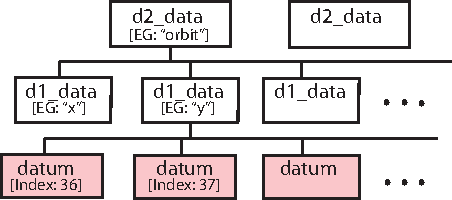
\includegraphics[width=4in]{data-tree.pdf}
  \caption[Data tree structure]
{A \vn{d2\_data} structure holds a set of \vn{d1\_data} structures. 
A \vn{d1\_data} structure holds an array of datums.}
  \label{f:data.tree}
\end{figure}

\index{d2_data}\index{d1_data}
The horizontal orbit at a particular BPM is an example of an
individual \vn{datum}.  For ease of manipulation, arrays of datums are
grouped into what is called a \vn{d1_data} structure. Furthermore,
sets of \vn{d1_data} structures are grouped into what is called a
\vn{d2_data} structure.  This is illustrated in
Figure~\ref{f:data.tree}.  For example, a \vn{d2_data} structure for
orbit data could contain two \vn{d1_data} structures --- one
\vn{d1_data} structure for the horizontal orbit data and another
\vn{d1_data} structure for the vertical orbit data. Each datum of,
say, the horizontal orbit \vn{d1_data} structure would then correspond
to the horizontal orbit at some point in the machine.

When issuing \tao commands, all the
data associated with a \vn{d2_data} structure is specified using the
\vn{d2_data} structure's \vn{name}.  The data associated with a
\vn{d1_data} structure is specified using the format
\begin{example}
  d2_name.d1_name
\end{example}
For example, if a \vn{d2_data} structure has the
name ``\vn{orbit}'', and one of its \vn{d1_data} structures has the
name ``\vn{x}'', then \tao commands that refer to the data in this
\vn{d1_data} structure use the name ``\vn{orbit.x}''. Sometimes there
is only one \vn{d1_data} structure for a given \vn{d2_data}
structure. In this case the data can be referred to simply by using
the \vn{d2_data} structure's name. The individual datums can be
referred to using the notation
\begin{example}
  <d2_name>.<d1_name>[<list_of_datum_indexes>]
\end{example}
For example, \vn{orbit.x[10]} refers to the horizontal orbit datum
with index 10. Notice that the beginning (lowest) datum index is user
selectable and is therefore not necessarily 1. 

It is important to note that the name given to \vn{d2_data} and \vn{d1_data}
structures is arbitrary and does not have to correspond to the 
type of data contained in the 
structures. In fact, a \vn{d1_data} array can contain heterogeneous data types.
Thus, for example, it is perfectly permissible (but definitely not recommended) 
to set up the data structures so that, say, \vn{orbit.x[10]} 
is the $a$-mode emittance at a certain element and \vn{orbit.x[11]}
is the $b$-mode beta function at the same element.

Ranges of data can be referred to using using a comma \vn{,} to
separate the indexes combined with the notation \vn{n1:n2} to specify
all the datums between \vn{n1} and \vn{n2} inclusive. For example
\begin{example}
  orbit.x[3:6,23]
\end{example}
refers to datums 3, 4, 5, 6, and 23. 

If multiple universes are present, then, as explained in
\sref{s:universe}, the prefix \vn{"@"} may be used to specify which
universe the data applies to. The general notation is
\begin{example}
  [<universe_range>]@<d2_name>.<d1_name>[<datum_index>]
\end{example}
Examples:
\begin{example}
  [2:4,7]@orbit.x ! The \vn{orbit.x} data in universes 2, 3, 4 and 7.
  [2]@orbit.x     ! The \vn{orbit.x} data in universe 2. 
  2@orbit.x       ! Same as "2@orbit.x".
  orbit.x         ! The \vn{orbit.x} data in the current viewed universe.
  -1@orbit.x      ! Same as "orbit.x".
\end{example}

As explained in Section~\sref{s:data.anatomy}, each individual datum
has a number of components. The syntax to refer to a component is:
\begin{example}
  d2_name.d1_name[datum_index]|component
\end{example}
For example:
\begin{example}
  orbit.x[3:10]|meas     ! The measured data values
\end{example}

In referring to datums, a ``\vn{*}'' can be used as a wild card to 
denote ``all''. Thus:
\begin{example}
  *@orbit.x       ! The \vn{orbit.x} data in all universes.
  *               ! All the data in the currently viewed universe.
  *.*             ! Same as "*"
  *@*             ! All the data in all the universes. 
  *@*.*           ! Same as "*@*"
  orbit.x[*]|meas ! All measured values of orbit.x
  orbit.x[]|meas  ! No values. That is, the empty set.
  orbit.x|meas    ! Same as orbit.x[*]|meas.
\end{example}
The last example shows that when referring to an entire block of data
encompassed by a \vn{d1_data} structure, the \vn{[*]} can be omitted.

%------------------------------------------------------------------------
\section{Anatomy of a Datum}
\label{s:data.anatomy}

Each datum has a number of quantities associated with it:
\begin{example}
  data_type        ! Character: Type of data: "orbit.x", etc.
  ele_name         ! Character: Name of lattice element where datum is evaluated.
  ele_start_name   ! Character: Name of starting lattice element in a range.
  ele_ref_name     ! Character: Name of reference lattice element.
  merit_type       ! Character: Type of constraint: "target", "max", etc.
  data_source      ! Character: How the datum is calculated. "lat", or "beam".
  ix_ele           ! Integer: Index of "ele" in the lattice element list.
  ix_ele_start     ! Integer: Index of "ele_start" in the lattice element list.
  ix_ele_ref       ! Integer: Index of "ele_ref" in the lattice element list.
  ix_ele_merit     ! Integer: Lattice index where merit is evaluated.
  ix_d1            ! Integer: Index number in d1_data structure
  ix_data          ! Integer: Index in the global data array
  ix_dModel        ! Integer: Row number in the dModel_dVar derivative matrix.
  ix_bunch         ! Integer: Bunch number to get the data from.
  meas             ! Real: Measured datum value. 
  ref              ! Real: Measured datum value from the reference data set.
  model            ! Real: Datum value as calculated from the model.
  design           ! Real: What the datum value is in the design lattice.
  old              ! Real: Used by \tao to save the model at some previous time.
  base             ! Real: The value as calculated from the base model.
  fit              ! Real: This value is not used by \tao.
  invalid          ! Real: The value used for delta_merit if good_model = False.
  delta_merit      ! Real: Diff used to calculate the merit function term 
  weight           ! Real: Weight for the merit function term
  merit            ! Real: Merit function term value: weight * delta^2
  s                ! Real: longitudinal position of ele.
  exists           ! Logical: Does the datum exist?
  good_model       ! Logical: Does the model  component contain a valid value?
  good_design      ! Logical: Does the design component contain a valid value?
  good_base        ! Logical: Does the base   component contain a valid value?
  good_meas        ! Logical: Does the meas   component contain a valid value?
  good_ref         ! Logical: Does the ref    component contain a valid value?
  good_user        ! Logical: Does the user want this datum used in optimization?
  good_opt         ! Logical: Can be used in Tao extensions.
  good_plot        ! Logical: Can be used in Tao extensions.
  useit_plot       ! Logical: Is this datum to be used in plotting?
  useit_opt        ! Logical: Is this datum to be used for optimization?
\end{example}
When running \tao, the \vn{show data}
(\sref{s:show}) command can be used to view the components of a datum. 
The \vn{set} command (\sref{s:set}) can be used to set some of these components.

%------------------------------------------------------------------------
\section{Datum values}
\label{s:datum.values}

\index{data!measured}\index{data!reference}\index{data!model}
\index{data!base}\index{data!design}
A given datum has six values associated it:
\vspace{-2ex}
\begin{description}
  \vspace{-1ex}
  \item[meas] \Newline 
The value of the datum as obtained from some measurement. This is the
target or limit value that is used when running the optimizer. When
doing lattice design, the measured value corresponds to a constraint
value (\ref{c:opti}).
  \vspace{-1ex}
  \item[base] \Newline
The datum value as calculated from the \vn{base} lattice (\sref{s:lattice}).
  \vspace{-0.5ex}
  \item[design] \Newline
The value of the datum as calculated from the \vn{design} lattice (\sref{s:lattice}).
  \vspace{-0.5ex}
  \item[fit] \Newline
The \vn{fit} value is not used by \tao directly and is available for use by custom code.
  \vspace{-0.5ex}
  \item[model] \Newline
The value of the datum as calculated from the \vn{model} lattice (\sref{s:lattice}).
  \vspace{-0.5ex}
  \item[old] \Newline
A datum value that was saved at some point in \tao's calculations. This value
can be ignored.
  \vspace{-0.5ex}
  \item[ref] \Newline
The reference datum value as obtained from some reference measurement. For example,
a measurement before some variable is varied could be designated as
the \vn{reference}, and the datum taken after the variation could be 
designated the \vn{measured} datum.
\end{description}

%------------------------------------------------------------------------
\section{Datums in Optimization}
\label{s:datum.opt}

When using optimization for lattice correction or lattice design
(\sref{c:opti}), Individual datums can be excluded from the process
using the \vn{veto} (\sref{s:veto}), \vn{restore} (\sref{s:restore}),
and \vn{use} (\sref{s:use}) commands. These set the \vn{good_user}
component of a datum. This, combined with the setting \vn{exists},
\vn{good_meas}, \vn{good_ref}, and \vn{good_opt}
determine the setting of \vn{useit_opt} which is the component that
determines if the datum is used in the computation of the merit
function. The settings of everything but \vn{good_user} is determined
by \tao

The \vn{exists} component is set by \tao to True if the datum exists
and False otherwise. A datum may not exist if the type of datum
requires the designation of an associated element but the
\vn{ele_name} component is blank. For example, a \vn{d1_data} array
set up to hold orbit data may use a numbering scheme that fits the
lattice so that , say, datum number 34 in the array does not
correspond to an existing BPM.

The \vn{good_model} component is set according to whether a datum
value can be computed from the \vn{model} lattice. For example, If a
circular lattice is unstable, the beta function and the closed orbit
cannot be computed. Similarly, the \vn{good_design} and \vn{good_base}
components mark whether the \vn{design} and \vn{base} values
respectively are valid.

When doing optimization, the \vn{delta_merit} component is set to the
\vn{delta} value used in computing the contribution to the merit
function (\sref{s:generalized.design}). If the datum's value cannot be
computed, that is, \vn{good_model} is False, or, if the design or base
values are being used in the merit calculation, \vn{good_base} or
\vn{good_design} is False, then the \vn{invalid} component is used for
\vn{delta_merit}.

\vn{good_meas} is set True if the \vn{meas} component value is set in
the data initialization file (\sref{s:init.data}) or is set using the
\vn{set} command (\sref{s:set}). Similarly, \vn{good_ref} is set True
if the \vn{ref} component has been set. \vn{good_ref} only affects the
setting of \vn{useit_opt} if the optimization is using reference data
as set by the global variable \vn{opt_with_ref} (\sref{s:globals}).

Finally \vn{good_opt} is meant for use in custom versions of \tao
(\sref{c:custom.tao}) and is always left True by the standard \tao code.

Example of using a \vn{show data} (\sref{s:show}) to check the logicals
in a datum:
\begin{example}
  Tao> show data 3@beta[1]

  Universe:   3
  %ele_name          = IP_L0
  %ele_ref_name      =
  %ele_start_name    =
  %data_type         = beta.a
      ... etc ...
  %exists            =  T
  %good_model        =  T
  %good_meas         =  F
  %good_ref          =  F
  %good_user         =  T
  %good_opt          =  T
  %good_plot         =  F
  %useit_plot        =  F
  %useit_opt         =  F
\end{example}
Here \vn{useit_opt} is False since \vn{good_meas} is False and
\vn{good_meas} is False since the \vn{meas} value of the datum (not
shown) was not set in the \tao initialization file.

%------------------------------------------------------------------------
\section{Data_source}
\index{data!data_source}
\label{s:data.source}

The \vn{data_source} component specifies where the data is 
coming from. Possible values are:
\begin{example}
  "beam"      ! Calculation using the beam distribution.
  "lat"       ! Calculation using the lattice.
\end{example}
If \vn{data_source} is set to \vn{"beam"}, the data is calculated
using multiparticle tracking.  If \vn{data_source} is set to
\vn{"lat"}, the data is calculated using the ``lattice'' which here
means everything {\em but} multiparticle tracking.  For example, the
\vn{"beam"} based calculation of the emittance uses the bunch sigma
matrix obtained through multiparticle tracking. The \vn{"lat"} based
calculation of the emittance uses radiation integrals.

Some data types may be restricted as to which \vn{data_source} is
possible. For example, a datum with \vn{data_type} set to
\vn{n_particle_loss} must use \vn{"beam"} for the \vn{data_source}. 
Table~\ref{t:data.types} lists which \vn{data_source} values are valid
for what data types.

%------------------------------------------------------------------------
\section{Datum Evaluation and Associated Lattice Elements}
\index{data!associated lattice elements}
\label{s:data.lat.ele}

Datums can be divided up into two classes. In one class are the datums
that are \vn{``local''}, like the beam orbit, which need to be evaluated at
either a particular point are evaluated over some finite region of the
machine. Other datums, like the emittance, are \vn{``global''} and do not
have associated evaluation points.

As mentioned, \vn{local} datums may be evaluated at a specific point
or over some evaluation region, an evaluation region is used when, for
example, the maximum or minimum value over a region is wanted. To
specify an evaluation point, an \vn{evaluation element} must be
associated with a datum. The evaluation point will be at the exit end
of this element. To specify an evaluation region, a \vn{start element}
must also be associated with a datum along with the \vn{evaluation
element}. The evaluation region is from the exit end of the \vn{start
element} to the exit end of the \vn{evaluation element}.

In addition to the \vn{evaluation element} and the \vn{start element},
a \vn{local} datum may have an associated \vn{reference element}.  A
\vn{reference element} is used as a fiducial point and the datum value
is calculated relative to that point. For example, a datum value may
be the position of the \vn{evaluation element} relative to the
position of the \vn{reference element}. The evaluation point of a
\vn{reference element} is the exit end of that element.

The components in a datum corresponding to the \vn{evaluation
element}, the \vn{reference element}, and the \vn{start element}.  are
shown in Table~\ref{t:datum.elements}.  These three elements may be
specified for a datum by either setting the name component or the
index component of the datum. Using the element index over the element
name is necessary when more than one element in the lattice has the
same name.

\begin{table}[htb]
\centering
\begin{tabular}{lll}
  \toprule
  &\multicolumn{2}{c}{\it Data Component} \\ \cmidrule{2-3}
  {\it Element} & {\it name} & {\it index} \\ \midrule
  Reference Element  & \vn{ele_ref_name}   & \vn{ix_ele_ref}   \\
  Start Element      & \vn{ele_start_name} & \vn{ix_ele_start} \\
  Evaluation Element & \vn{ele_name}       & \vn{ix_ele}       \\ \bottomrule
\end{tabular}
\caption[The three lattice elements associated with a datum.]
{The three lattice elements associated with a datum may be
specified in the datum by setting the appropriate name component or by 
setting the appropriate index component.}
\label{t:datum.elements}
\end{table}

If a datum has an associated \vn{evaluation} element, but no
associated \vn{start} or \vn{reference} elements, the \vn{model} value
of that datum is the value of the \vn{data_type} at the \vn{evaluation}
element. For example, if a datum has:
\begin{example}
  data_type      = "orbit.x"
  ele_name       = "q12"
\end{example}
here the \vn{model} value of this datum will be the horizontal orbit
at the element with name \vn{q12}.

If a datum has an associated \vn{start} element, specified by either
setting the \vn{ele_start_name} or \vn{ix_ele_start} datum components, the
datum is evaluated over a region from the exit end of the \vn{start} element
to the exit end of \vn{evaluation} element. For example, if a datum has:
\begin{example}
  data_type      = "beta.a"
  ele_name       = "q12"
  ele_start_name = "q45"
  merit_type     = "max"
\end{example}
then the \vn{model} value of this datum will be the maximum value of
the a-mode beta function in the region from the exit end of the
element with name \vn{q12} to the exit end of the element with name
\vn{q45}. Notice that when a range of elements is used, a
\vn{merit_type} of \vn{target} does not make sense. 

Typically, in evaluating a datum over some region to find the maximum
or minimum, \tao will only evaluate the datum at the ends of the
elements with the assumption that this is good enough. If this is not
good enough, marker elements can be inserted into the lattice at
locations that matter. For example, the maximum or minimum of the beta
function typically occurs near the middle of a quadrupole so inserting
marker elements in the middle of quadrupoles will improve the accuracy
of finding the extremum beta.

If a datum has an associated \vn{reference} element, specified by either
setting the \vn{ele_ref_name} or \vn{ix_ele_ref} datum components, the
\vn{model} value of the datum is the value at the \vn{evaluation} element (or the value
over the range \vn{ele_start} to the \vn{evaluation} element if \vn{ele_start} is
specified), minus the \vn{model} value at \vn{ele_ref}. For example,
if a datum has:
\begin{example}
  data_type      = "beta.a"
  ele_name       = "q12"
  ele_start_name = "q45"
  ele_ref_name   = "q1"
  merit_type     = "max"
\end{example}
then the \vn{model} value of the datum will be the same as the
previous example minus the value of the a-mode beta function at the
exit end of element \vn{q1}. There are a number of exceptions to the
above rule and datum types treat the \vn{reference} element in a different
manner. For example, the \vn{r.} data type uses the \vn{reference} element
as the starting point in constructing a transfer matrix.

%------------------------------------------------------------------------
\section{Tao Data Types}\index{data!data Types}
\label{s:data.types}

The \vn{data_type} component of datum specifies what type of data the
datum represents. For example, a datum with a \vn{data_type} of
\vn{orbit.x} represents the horizontal orbit. Table~\ref{t:data.types} lists
what data types \tao knows about.

It is important to note the difference between the \vn{d2.d1} name
that is used to refer to a datum and the actual type of data, given by
\vn{data_type}, of the datum. The \vn{d2.d1} name is arbitrary and is
specified in the \tao initialization file (\sref{s:init.data}). Often,
these names do reflect the actual type of data. However, there is no
mandated relationship between the two. For example, it is perfectly
possible to set create a data set with a \vn{d2.d1} name of
\vn{orbit.x} to hold, say, global floor position data. In fact, the
datums in a given \vn{d1} array do not all have to be of the same
type. Thus the user is free to group data as s/he sees fit.

Description of the data types:

  \begin{description}
  \index{apparent_emit.}
  \item[apparent_emit.] \Newline
The apparent emittance is the emittance that one would calculate based
upon a measurement of the beam size\cite{b:emit}. It can be useful to
compare this to the true normal mode emittance. Also See the
\vn{norm_apparent_emit}, \vn{emit.} and \vn{norm_emit.} data types.
With \vn{data_source} set to \vn{"beam"}, \vn{apparent_emit.x} is
\begin{equation}
  E_x = \frac{\sigma_{xx} - \eta_x^2 \, \sigma_{p_zp_z}}{\beta_a}
\end{equation}
with a similar equation for \vn{apparent_emit.y}. Here $\sigma$ is the beam size matrix
\begin{equation}
  \sigma_{r_1r_2} \equiv \left< r_1 \, r_2 \right>
\end{equation}
With \vn{data_source} set to \vn{"lat"}, The apparent emittance is
calculated from the true normal mode emittance and the Twiss
parameters (Cf.~ Eqs (4) and (5) of \cite{b:emit}).

  \index{beta.}
  \item[beta.] \Newline
\vn{beta.a} and \vn{beta.b} are the lattice beta functions. \vn{beta.x} and
\vn{beta.y} are beam projected beta functions defined by
\begin{equation}
  \beta.x = \frac{<x^{2}>}{\sqrt{<x^{2}> <x'^{2}> - <x x'>^{2}}}.
\end{equation}
where the average \vn{<>} is over all the particles in the beam.

Note: If the beta function is calculated from the beam distribution,
the emittance must be non-zero.

  \index{element_attrib.}
  \item{element_attrib.} \Newline
The \vn{element_attrib.<attrib_name>} data type is associated with the
lattice element attribute named \vn{<attrib_name>}. For any given
element, if \vn{<attrib_name} is not associated with the element, the
value of the datum is zero.

  \index{emit.}
  \item[emit.] \Newline
The \vn{emit.} data type covers two types of
``emittance''. \vn{emit.a}, \vn{emit.b}, and \vn{emit.c} are the true
normal mode (eigen) emittances. \vn{emit.x}, \vn{emit.y}, and
\vn{emit.z} are the ``projected'' emittances\cite{b:emit}. 
For a linear lattice, the emittance varies along the length
of the line while for a circular lattice there is a single emittance
number. 

With \vn{data_source} set to \vn{"beam"}, the emittance is calculated
from the beam sigma matrix. For the eigen emittance this involves the
standard normal mode decomposition. For the projected emittance, the
formula for $\epsilon_x$ is
\begin{equation}
  \epsilon_x = \sqrt{ \wt\sigma_{xx} \, \wt\sigma_{p_xp_x} - \wt\sigma_{xp_x}^2}
\end{equation}
With a similar equation for $\epsilon_y$. Here $\wt\sigma$ is the energy normalized
beam size:
\begin{equation}
  \wt\sigma_{xx} = \langle x \, x \rangle - 
  \frac{\langle x \, p_z \rangle \, \langle x \, p_z \rangle}{\langle p_z \, p_z \rangle}
\end{equation}
with similar definitions for the other $\wt\sigma$ components. 
Note that the projected emittance is sometimes defined using
$x'$ and $y'$ in place of $p_x$ and $p_y$. However, in the vast
majority of cases, this does not appreciably affect the numeric
results.

With \vn{data_source} set to \vn{"lat"}, the normal mode emittance is calculated
using the standard radiation integrals.

See also the \vn{norm_emit.}, \vn{apparent_emit.}, and
\vn{norm_apparent_emit.} data types.

  \index{expression: }
  \item[expression:] \Newline
The \vn{expression:} The data type can be an expression (\sref{s:arithmetic.exp}).
In this case the \vn{data_type} must begin with the string ``\vn{expression:}''.
For example:
\begin{example}
  datum(i)%data_type = "expression: 1@lat::q10w[beta_a] - 2@lat::q10w[beta_a]"
\end{example}
With this, the value of the datum will be the difference between
the a-mode beta at element \vn{q10w}
for universe 1 and universe 2. In this example,
the source of both terms in the expression is explicitly given as \vn{lat}.
This is not necessary if the \vn{datum%data_source} is set to \vn{lat}
\begin{example}
  datum(i)%data_type = "expression: 1@q10w[beta_a] - 2@q10w[beta_a]"
  datum(i)%data_source = "lat"
\end{example}
An expression can also be used as the
\vn{default_data_type}. In this case, the 
evaluation point is implicit. For example:
\begin{example}
  default_data_source = "dat"
  default_data_type = "expression: 1@beta.a - 2@beta.a"
\end{example}
which is equivalent to:
\begin{example}
  default_data_type = "expression: 1@dat::beta.a - 2@dat::beta.a"
\end{example}

To be valid, if an expression has a term with a \vn{dat} source, the
expression must be evaluated after the \vn{dat} source components are
evaluated. Data evaluation is done universe by universe starting with
universe 1, then universe 2, etc. Within a given universe, the order
of evaluation can be complicated but in this case a datum using an
expression will always be evaluated after any datum that appears
earlier in the initialization file.  In the last example above, the
expression terms involve an evaluation of \vn{beta.a} in universe 2.  
Therefore, this expression datum should
be in universe 2 or higher. Notice that while all datums must be
assigned a universe, in this case, since all the terms explicitly give
a universe number, the value of the datum will be independent of the
universe it is in.

  \index{floor.}
  \item[floor.] \Newline
This is the global floor position at the exit end of evaluation element. See the
\bmad manual for details on the global coordinate system. See also
\vn{rel_floor.}.

  \index{n_particle_loss}
  \item[n\_particle\_loss] \Newline
If the reference element is not specified, \vn{n_particle_loss} gives
the number of particles lost at the evaluation element. If the
reference element is specified, \vn{n_particle_loss} gives the
cumulative loss between the exit end of the reference element and the
exit end of the evaluation element. That is, this sum does not count
any losses at the reference element itself. If neither reference nor
evaluation element is given then the total number of lost particles is
given.

  \index{norm_apparent_emit.}
  \item[norm_apparent_emit.] \Newline
The \vn{norm_apparent_emit.} data type is the energy normalized
apparent emittance. The normalization is the standard gamma factor:
\Begineq
  E_{norm} = \gamma \, E
\Endeq
See the \vn{apparent_emit.} data type for more details.

  \index{norm_emit.}
  \item[norm_emit.] \Newline
The \vn{norm_emit.} data type is the energy normalized
emittance. The normalization is the standard gamma factor:
\Begineq
  \epsilon_{norm} = \gamma \, \epsilon
\Endeq
See the \vn{apparent_emit.} data type for more details.


  \index{periodic.tt.}
  \item[periodic.tt.] \Newline
This is like the \vn{tt.} datum except here the terms are from the
periodic Taylor map defined by
\Begineq
  T_p \equiv (T_0 - I_4)^{-1}
\Endeq
Here $T_p$ is the
periodic map, $T_0$ is the one-turn map from some point back to that
point, and $I_4$ is a linear map defined by the matrix
\Begineq
  I_4 \equiv 
    \begin{pmatrix}
      1 &   &   &   &   &   \\
        & 1 &   &   &   &   \\
        &   & 1 &   &   &   \\
        &   &   & 1 &   &   \\
        &   &   &   & 0 &   \\
        &   &   &   &   & 0
    \end{pmatrix}
\Endeq
The periodic map give information about the closed orbit, dispersion,
etc. For example, the zeroth order terms are the closed orbit, the r16
term gives the horizontal dispersion, etc.

If a reference lattice element is specified, the map $T_0$ will be
the transfer map from the reference element to the evaluation element.

Note: If the reference element is not specified, or if the reference
element is the same as the evaluation element, this data type cannot
be used with a linear lattice.

  \index{phase.}
  \item[phase.] \Newline
This is the betatron phase.  If a \vn{d1_data} array has a set of
\vn{phase} datums, and if the reference element is {\em not}
specified, the average phase used for optimizations ($D$ in
\Eq{miwdjw}) and plotting for all the datums within a \vn{d1_data}
array are set to zero by adding a fixed constant to all the datums.
This is done since, without a reference point that defines a zero
phase, the overall average phase is arbitrary and so the average phase
is taken in \tao to be zero. This can be helpful in optimizations
since one does not have to worry about arbitrary offsets between the
\vn{model} and \vn{measured} values. If the reference element is
specified then there is no arbitrary constant in the evaluation.

  \index{rad_int.}
  \item[rad_int, rad_int1] \Newline
The \vn{rad_int.} datums are the radiation integrals from the start of
the lattice. The \vn{rad_int1.} datums are the radiation integrals on
an element-by-element basis. That is, if \vn{ele_ref} is not specified,
\vn{rad_int.} will give the radiation integral from the start of the 
lattice through the evaluation element, and \vn{rad_int1.} will give
the radiation integral integrated over just the evaluation element.

  \index{ref_time}
  \item[ref_time] \Newline
This is the time the reference particle passes the exit end of the element.
If the particle is ultra-relativistic then this is just $c * s$ where $s$
is the longitudinal distance from the start of the lattice.

  \index{rel_floor.}
  \item[rel\_floor.] \Newline
This is the global floor position at the exit end of the evaluation
element relative to the exit end of the reference element in a global
coordinate system where the exit end of the reference element is taken to be at
\vn{x = y = z = theta = phi = 0}. See the \bmad manual for details on
the global coordinate system. See also \vn{floor.}.

  \index{t. tt.} 
  \item[t. tt.] \Newline
The \vn{t} and \vn{tt} data types give terms of the Taylor map between
two points. The difference between \vn{t.} and \vn{tt.} is that
\vn{t.} is restricted to exactly three indices and \vn{tt.} is
not. \vn{t.} is superfluous but is keep for backwards compatibility.

Calculation of \vn{t.} and \vn{tt.} datums involve symplectic
integration through lattice elements. One point to be kept in mind is
that results will be dependent upon the integration step size through
an element set by the \vn{ds_step} attribute of that element (see the
\bmad manual for more details). When a smooth curve
(\sref{s:template}) is plotted for \vn{t} and \vn{tt} data types, and
the longitudinal (\vn{"s"}) position is used for the x-axis, the
integration step used in generating the points that define this curve
will be decreased if the s-distance between points is smaller than
the \vn{ds_step}.  In this case, discrepancies between the plot and
datum values may be observed.

  \index{unstable.orbit}
  \item[unstable.orbit] \Newline
The \vn{unstable.orbit} datum is used for linear lattices in an
optimization to avoid unstable solutions (\sref{s:generalized.design}).

For single particle tracking, the value of an \vn{unstable.orbit}
datum is zero if the tracked particle survives (has not been lost) up
to the evaluation element and, if it has been lost, is set to
\Begineq
 1 + i_{\mbox{ele}} - i_{\mbox{lost}} + \frac{1}{2}
 \left[ \tanh\left( \frac{r_{orbit}}{r_{lim}} - 1 \right) - E \right]
\Endeq
where $i_{\mbox{ele}}$ is the index of the evaluation element in the
lattice and $i_{\mbox{lost}}$ is the index of the element where the
particle was lost. In the above equation, $E$ is the function
\Begineq
  E = 
  \begin{cases}
    1 & \text{if the particle is lost at the exit end of the element.} \\
    0 & \text{if the particle is lost at the entrance end of the element.}
  \end{cases}
\Endeq
In the abouve equation, $r_{orbit}$ is the particle amplitude at the
point of loss and $r_{lim}$ is the aperture limit. The form of the
above equation has been choisen so that the datum value will be
monotonic with increasing stability.

The default for the evaluation element, if \vn{ele_name} nor
\vn{ix_ele} is not specified, is to use the last element in the
lattice. 

When tracking beams, the value of \vn{unstable.orbit} is the averaged
value over all particles in the bunch.

  \index{unstable.ring}
  \item[unstable.ring] \Newline
\vn{unstable.ring} is used for storage rings. The value of an
\vn{unstable.ring} datum is zero if the ring is stable and set to the
largest growth rate of all the normal modes of oscillation if the ring
is unstable. \vn{unstable.ring} is used in an optimization to avoid
unstable solutions (\sref{s:generalized.design}).

\begin{figure}
  \centering
  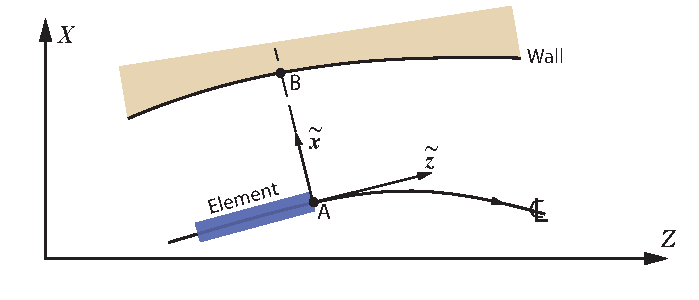
\includegraphics[width=5in]{building-wall-constraint.pdf}
  \caption[Building wall datum]
{A \vn{wall.} datum is a measure of the distance between the
centerline of a machine and the walls of the containment building.}
  \label{f:wall.constraint}
\end{figure}

  \index{wall.}
  \item[wall.] \Newline
The \vn{wall.} data types are used to constrain the shape of a machine
to fit inside a building's walls (\sref{s:building.wall}). The general
layout is shown in Figure~\ref{f:wall.constraint}. The machine
centerline is projected onto the horizontal $(Z, X)$ plane in the
Global (floor) coordinate system. Point \vn{A} is an evaluation point
at the exit end of some element. $\wt z$ is the projection of the
local $z$-axis onto the $(Z, X)$ plane and $\wt x$ is the coordinate
in the $(Z, X)$ plane perpendicular to $\wt z$. In the typical
situation, where a machine is planer (no out-of-plane bends), the $\wt
z$-axis corresponds to the local $z$-axis and the $\wt x$-axis
corresponds to the $x$-axis (see the \bmad manual for an explanation
of local and global coordinate systems).

The distance from the machine at point \vn{A} to the wall is defined
to be the distance from \vn{A} to a point \vn{B} on the wall where
point \vn{B} is along the $\wt x$ axis (has $\wt z = 0$) as shown in
Figure~\ref{f:wall.constraint}.

By definition, the \vn{``left side''} of the machine corresponds to be
the $+\wt x$ side and the \vn{``right side''} corresponds to be the
$-\wt x$ side. That is, left and right are relative to someone looking
in the same direction as the beam is propagating. Correspondingly,
there are two wall data types: \vn{wall.left_side} and
\vn{wall.right_side}. With the \vn{wall.left_side} data type, the
datum value is positive if point \vn{B} is on the left side and
negative if on the right. Vice versa for a \vn{wall.right_side} datum.
If there are multiple wall points \vn{B}, that is, if there are
multiple points on the wall with $\wt z = 0$, the datum value will be
the minimum value. Notice that only wall sections that have a
\vn{constraint} matching the datum will be used when searching for
possible points \vn{B}. If there are no wall points with $\wt z = 0$,
the datum value is set to a large number.

For \vn{wall} data there can be no reference element since this does
not make sense.

  \index{wire.}
  \item[wire] \Newline
\vn{wire} data simulates the measurement of a wire scanner. The angle
specified is the angle of the wire with respect to the horizontal
axis. The measurement then measures the second moment $<uu>$ along an
axis which is 90 degrees off of the wire axis. For example,
\vn{wire.90} is a wire scanner oriented in the vertical direction and
measures the second moment of the beam along the horizontal axis,
$<xx>$. The resultant data is not the beam size, but the beam size
squared.

  \end{description}


\index{data!calculation method}
\index{unstable.orbit}\index{beta}\index{alpha}\index{eta}\index{eta}
\index{etap}\index{phase}\index{orbit}\index{wire}\index{building wall}\index{spin}
\index{cbar}\index{coupling}\index{floor}\index{r}\index{t}\index{tt}
\index{rad_int.i5a_e6}\index{rad_int.i5b_e6}\index{s_position}\index{e_tot}
\index{unstable.ring}\index{emittance}\index{chrom}\index{norm_emittance}
\index{sigma}\index{dpx_dx}\index{dpy_dy}\index{dpz_dz}\index{dpa_da}
\index{dpb_db}\index{rad_int.i1}\index{rad_int.i2}\index{rad_int.i2_e4}
\index{rad_int.i3}\index{rad_int.i3_e7}

%----------------------------------------------------------------------------------------------

{\tt\small
\begin{longtable}{lll} 
  \caption{Predefined Data Types in Tao}
  \label{t:data.types}
  \\ \hline

  {\it Data\_Type}                    & {\it Description}                             & Source    \\ \hline\hline 
  \endfirsthead

  \caption[]{(continued)} \\ \hline
  {\it Data\_Type}                    & {\it Description}                             & source    \\ \hline\hline 
  \endhead

  alpha.a, alpha.b                    & Normal-Mode alpha function                    & lat       \\ \hline 
  apparent\_emit.x, apparent\_emit.y  & Apparent emittance                            & beam, lat \\ \hline
  beta.a, beta.b, beta.c              & Normal-mode beta function                     & beam, lat \\ \hline 
  beta.x, beta.y  beta.z              & Projected beta function                       & beam, lat \\ \hline 
  bpm\_orbit.x, bpm\_orbit.y          & Measured orbit                                & lat       \\ \hline
  bpm\_phase.a, bpm\_phase.b          & Measured betatron phase                       & lat       \\ \hline
  bpm\_eta.x, bpm\_eta.y              & Measured dispersion                           & lat       \\ \hline

  \begin{tabular}{@{}l}
    bpm\_k.22a, bpm\_k.12a, \\
    bpm\_k.11b, bpm\_k.12b
  \end{tabular}                       & Measured coupling                             & lat       \\ \hline

  \begin{tabular}{@{}l}
    bpm\_cbar.22a, bpm\_cbar.12a, \\
    bpm\_cbar.11b, bpm\_cbar.12b
  \end{tabular}
                                      & Measured coupling                             & lat       \\ \hline

  cbar.11, cbar.12, cbar.21, cbar.22
                                      & Coupling                                      & lat       \\ \hline 

  chrom.a, chrom.b                    & Chromaticity for a ring                       & lat       \\ \hline

  dpx\_dx, dpx\_dy, etc.              & Bunch <x px> / <$x^2$> \& Etc...              & beam      \\ \hline 

  e\_tot                              & Beam total energy (eV)                        & lat       \\ \hline

  element\_attrib.<attrib\_name>      & lattice element attribute                     & lat       \\ \hline

  emit.a, emit.b, emit.c              & Emittance                                     & beam, lat \\ \hline

  eta.x, eta.y, eta.z                 & Lab Frame dispersion                          & beam, lat \\ \hline 
  eta.a, eta.b                        & Normal-mode dispersion                        & beam, lat \\ \hline 
  etap.x, etap.y                      & Lab Frame dispersion derivative               & beam, lat \\ \hline 
  etap.a, etap.b                      & Normal-mode dispersion derivative             & beam, lat \\ \hline 

  expression: <arithmetic expression> & See the text                                  & lat       \\ \hline 

  floor.x, floor.y, floor.z, floor.theta 
                                      & Global (``floor'') position                   & lat       \\ \hline 

  gamma.a, gamma.b                    & Normal-mode gamma function                    & lat       \\ \hline 

  rad\_int.i1                         & I1 radiation integral                         & lat       \\ \hline
  rad\_int.i2                         & I2 radiation integral                         & lat       \\ \hline
  rad\_int.i2\_e4                     & Energy normalized I2 radiation integral       & lat       \\ \hline
  rad\_int.i3                         & I3 radiation integral                         & lat       \\ \hline
  rad\_int.i3\_e7                     & Energy normalized I3 radiation integral       & lat       \\ \hline
  rad\_int.i5a, rad\_int.i5b          & I5 radiation integrals                        & lat       \\ \hline
  rad\_int.i5a\_e6, rad\_int.i5b\_e6  & Energy normalized I5 radiation integral       & lat       \\ \hline

  k.11b, k.12a, k.12b, k.22a          & Coupling                                      & lat       \\ \hline 
  momentum                            & Momentum: P*C\_light (eV)                     & lat       \\ \hline
  momentum\_compaction                & Momentum compaction factor                    & lat       \\ \hline

  \begin{tabular}{@{}l}   
    multi\_turn\_orbit.x, multi\_turn\_orbit.px \\ 
    multi\_turn\_orbit.y, multi\_turn\_orbit.py \\
    multi\_turn\_orbit.z, multi\_turn\_orbit.pz \\
  \end{tabular}                       & Bunch size                                    & lat       \\ \hline 

  n\_particle\_loss                   & Number of particles lost                      & beam      \\ \hline 

  \begin{tabular}{@{}l}
    norm\_apparent\_emit.x \\
    norm\_apparent\_emit.y 
  \end{tabular}                       & Normalized apparent emittance                 & beam, lat \\ \hline
  norm\_emit.a, norm\_emit.b, norm\_emit.c 
                                      & Normalized beam emittance                     & beam, lat \\ \hline 
  norm\_emit.x, norm\_emit.y, norm\_emit.z
                                      & Energy Normalized projected emittance         & beam, lat \\ \hline 

  orbit.x, orbit.y, orbit.z           & Orbit                                         & beam, lat \\ \hline 
  orbit.px, orbit.py, orbit.pz       & Momenta                                       & beam, lat \\ \hline 
  orbit.amp\_a, orbit.amp\_b          & ``Invariant'' amplitude                       & lat       \\ \hline 
  orbit.norm\_amp\_a, orbit.norm\_amp\_b  
                                      & Energy normalized ``invariant'' amplitude     & lat       \\ \hline 

  periodic.tt.$ijklm\ldots$ \hspace{10pt} $1 \le i,j,k,\ldots \le 6$   
                                      & Taylor term of the periodic map.              & lat       \\ \hline 

  phase.a, phase.b                    & Betatron phase                                & lat       \\ \hline 

  phase\_frac.a, phase\_frac.b        & \begin{tabular}{@{}l}
                                         Fractional betatron phase \\       
                                         $-\pi < \phi_{\mbox{frac}} < \pi$ \\
                                       \end{tabular}                                 & lat        \\ \hline 

  phase\_frac\_diff                   & \begin{tabular}{@{}l}
                                         Fractional betatron phase \\
                                        difference (a-b) $-\pi < d\phi_{\mbox{frac}} < \pi$
                                       \end{tabular}                                 & lat       \\ \hline 

  photon.intensity_x, photon.intensity_y
                                      & Photon intensity                              & beam, lat \\ \hline
  photon.intensity                    & Photon total intensity                        & beam, lat \\ \hline 
  photon.phase_x, photon.phase_y      & Photon phase                                  & beam, lat \\ \hline

  r.$ij$ \hspace{10pt} $1 \le i,j \le 6$
                                      & Term in linear transfer map                   & lat       \\ \hline 

  ref\_time                           & Reference time                                & beam, lat \\ \hline

  \begin{tabular}{@{}l}   
    rel\_floor.x, rel\_floor.y, \\
    rel\_floor.z, rel\_floor.theta \\
  \end{tabular}                       & Relative global (``floor'') position          & lat       \\ \hline 

  s\_position                         & longitudinal length constraint                & lat       \\ \hline 

  \begin{tabular}{@{}l}   
    sigma.x, sigma.y, sigma.z \\ 
    sigma.px, sigma.py, sigma.pz
  \end{tabular}                       & Bunch size                                    & beam, lat \\ \hline 

  spin.polarization, spin.theta, spin.phi
                                      & Particle spin                                 & beam, lat \\ \hline 
  time                                & Particle time (sec)                           & lat       \\ \hline
  t.$ijk$ \hspace{10pt} $1 \le i,j,k \le 6$
                                      & Term in 2\Nd order transfer map               & lat       \\ \hline 
  tt.$ijklm\ldots$ \hspace{10pt} $1 \le i,j,k,\ldots \le 6$
                                      & Term in n\Th order transfer map               & lat       \\ \hline 

  tune.a, tune.b                      & Tune                                          & lat       \\ \hline 
  unstable.orbit                      & Nonzero if particles are lost in tracking     & lat       \\ \hline
  unstable.ring                       & Nonzero if a ring is unstable                 & lat       \\ \hline
  wire.<angle>                        & Wire scanner at wire angle <angle>            & beam      \\ \hline
  wall.left\_side, wall.right\_side   & Building wall constraint                      & lat       \\ \hline
\end{longtable}
}

\chapter{Plotting}
\index{plotting}
\label{c:plotting}

\begin{figure}[b]
  \centering
  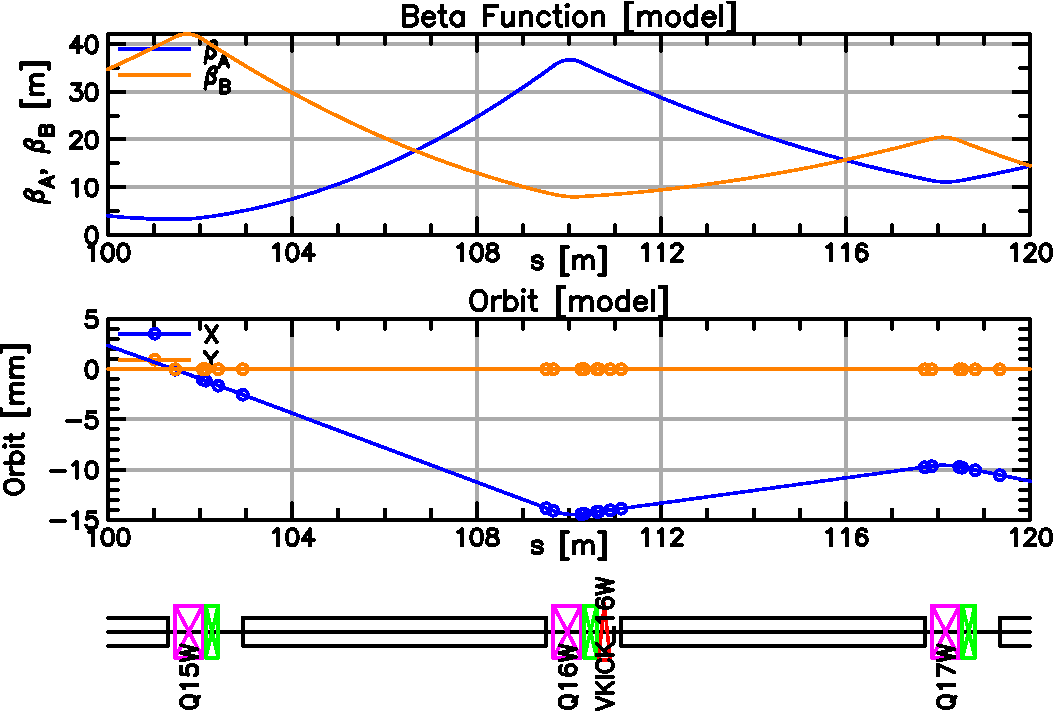
\includegraphics[width=4.5in]{plot-typical.pdf}
  \caption[An example of a plot display.]
{An example of a plot display. In this example there are three graphs: A graph displaying the beta
function, a graph displaying the orbit, and a graph displaying the ``lattice layout'' which shows
the longitudinal positions of lattice elements.}
  \label{f:plot.typ}
\end{figure}

\tao has a graphical display window within which such things as lattice functions, machine layout,
beam positions, etc., can be plotted. An example is shown in \fig{f:plot.typ} where there are plots
of the beta function and orbit along with a ``lattice layout which shows the longitudinal positions
of lattice elements. 

\tao organizes the display window using a number of concepts which are explained in the 
sections below
\begin{example}
  plot_page     ! The display window containing the graphics (\sref{s:plot.page.def}).
  regions       ! A set of rectangles on the plot_page that plots can be put in (\sref{s:region.def}).
  plot          ! A collection of graphs (\sref{s:plot.def}).
  box           ! Rectangular area within a plot that a graph is placed in (\sref{s:box.def}).
  graph         ! A diagram of some sort (\sref{s:graph.def}).
  curve         ! Data displayed within a \vn{graph} (\sref{s:curve.def}).
\end{example}

Underlying all this is the \vn{quick_plot} software toolkit (\sref{s:quick.plot}) which was developed
for \bmad and \tao for graphics plotting.

%-----------------------

\begin{figure}[bt]
  \centering
  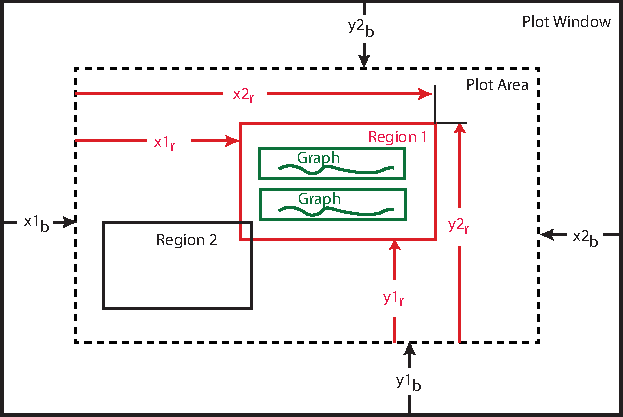
\includegraphics{plot-page.pdf}
  \caption[The plot window.]{The \vn{plot page} is the entire display window area. The \vn{plot area} 
is the region within the boarders of the \vn{plot page} within which ``\vn{regions}'' are
placed. The location of a \vn{region} is defined by four offsets with respect to the \vn{plot
area}. Regions may overlap.}
  \label{f:plot.page}
\end{figure}

%-----------------------------------------------------------------
\section{Plot Page}
\label{s:plot.page.def}

The \vn{plot page}, sometimes called the \vn{plot window}, refers to the window or the corresponding
printed graphics page where graphics are displayed. A \vn{plot page} is shown schematically in
\fig{f:plot.page}. Parameters associated with the \vn{plot page} are discussed in
\sref{s:plot.page}.  These parameters may be set in an initialization file or may be set on the \tao
command line using the \vn{set plot_page} (\sref{s:set.plot.page}) command. Examples:
\begin{example}
  set plot_page text_height = 11  ! 11 point font size
  set plot_page border%x1 = 0.2   ! Set left page border to 20% of width.
\end{example}

The size of the \vn{plot page} is set by the \vn{plot_page%size} parameter which is an array of two
numbers which set the width and height. The \vn{plot page} size can also be set when invoking \tao
using the \vn{-geometry} option (\sref{s:command.line})
\begin{example}
  > tao -lattice lat.bmad -geometry 300x500
\end{example}
This starts \tao with the \vn{plot page} size set to 300 points wide by 500 points high. It is also
sometimes convenient to start \tao without the plotting window. In this case, the \vn{-noplot} option
can be used on the startup command line. In a \tao initialization file, display of the plot window can be set
using the \vn{global%plot_on} parameter set in the \vn{tao_params} namelist (\sref{s:globals}).

The \vn{plot page} has a border within which \vn{regions} (\sref{s:region.def}) are defined. The area withing
the plot page border is called the \vn{plot area}

The \vn{show plot -page} (\sref{s:show.plot}) command may be used to view the page parameters.

%-----------------------------------------------------------------
\section{Region}
\label{s:region.def}

The \vn{plot area} is the area within the border of the \vn{plot page} as shown in
\fig{f:plot.page}.  In this \vn{plot area}, ``\vn{regions}'' can be defined which are invisible
rectangles where a \vn{plot} (\sref{s:plot.def}) can be placed. This is shown schematically in
\fig{f:plot.page}. Each region has a name and four numbers which specifies the location of the
region within the plot area. Regions may be defined by the user. In addition, for convenience, \tao
will define a number of regions. \tao defined regions will either begin with the letter ``\vn{r}''
or begin with the string ``\vn{layout}'' or the string ``\vn{scratch}''. Regions may overlap. How to
define regions is explained in \sref{s:plot.page}. The \vn{show plot} command will show the region
list. Example:
\begin{example}
  Tao> show plot

Plot Region         <-->  Plot                 x1    x2    y1    y2     Visible
-----------               -----------------------------------------------------
layout              <-->  lat_layout          0.00  1.00  0.00  0.15         T
r11                 <-->                      0.00  1.00  0.15  1.00
r12                 <-->                      0.00  1.00  0.58  1.00
r22                 <-->                      0.00  1.00  0.15  0.58
r13                 <-->  beta                0.00  1.00  0.72  1.00         T
r23                 <-->  dispersion          0.00  1.00  0.43  0.72         T
r33                 <-->  orbit               0.00  1.00  0.15  0.43         T
r14                 <-->                      0.00  1.00  0.79  1.00
\end{example}
The \vn{Plot} column shows what \vn{plot} (if any) is associated with the region
(\sref{s:plot.def}). The next four columns show the values of \vn{x1}, \vn{x2}, \vn{y1}, and \vn{y2}
set for the region. As shown in \Sref{s:plot.page}, \vn{x1} and \vn{x2} are the offsets from the
left \vn{plot area} edge to the left and right edges of the region. Similarly, \vn{y1} and \vn{y2}
are the offsets from the bottom edge of the \vn{plot area} to the bottom and top edges of the
region. \vn{x1} and \vn{x2} are normalized by the \vn{plot area} width and \vn{y1} and \vn{y2} are
normalized by the \vn{plot area} height so all four numbers should be in the range $[0, 1]$.  Using
the above example, the \vn{r23} region spans the full width of the \vn{plot area} (since \vn{x1} = 0
and \vn{x2} = 1), and occupies approximately the middle third vertically of the \vn{plot area}
(since \vn{y1} = 0.43 and \vn{y2} = 0.72).

The last column in the above shows if the \vn{plot} associated with the \vn{region} is
visible. Normally everything is visible. Invisibility is used in some special cases. For example,
when using a Graphical User Interface (GUI).

The \vn{set region} command can be used to set region parameters. Example:
\begin{example}
  set region r13 y1 = 0.8  ! Sets lower edge vertical position
\end{example}

%-----------------------------------------------------------------
\section{Plot}
\label{s:plot.def}

A \vn{plot} is essentially a collection of \vn{graphs}. This is shown schematically in
\fig{f:plot.plot} which shows a plot with two graph side by side.

Plots are divided into two groups. A \vn{template} plot defines how a \vn{displayed} plot is to be
constructed. That is, a \vn{template} plot defines what the associated \vn{graphs} are, defines
graph placement within the plot, etc. When a \vn{template} plot is \vn{placed} in a \vn{region},
either by using the \vn{place} command (\sref{s:place}) or by placement defined in an initialization
file (\sref{s:plot.page}), the information of the \vn{template} is copied in order to construct a
\vn{displayed} plot. A given \vn{template} plot may be placed in multiple \vn{regions} to give
multiple \vn{displayed} plots and then, using \vn{set} commands, the data displayed in each of these
plots may be manipulated separately. For example, one displayed orbit plot could show the orbit of
the \vn{model} lattice while another orbit plot could show the orbit difference between the
\vn{model} and \vn{design} lattices. When a \vn{plot} is displayed in a given \vn{region},
everything drawn is scaled to the region size.

Use the \vn{show plot} to see what displayed plots are associated with what regions. Use the
\vn{show plot -templates} command to see a list of \vn{template} plots. \tao defines a number of
default \vn{template} plots. Section~\sref{s:template} discusses how to define custom template
plots in an initialization file. Use the \vn{set plot} command (\sref{s:set.plot}) to modify either
\vn{template} or \vn{displayed} plots.

All plots have a name. A \vn{displayed} plot will inherit the same name of the \vn{template} plot it
came from. If a given \vn{template} plot is used to create multiple \vn{displayed} plots. All of
these plots will have the same name. A \vn{displayed} plot can also be referred to by using the
associated \vn{region} name. This can be used to remove ambiguity if there are multiple
\vn{displayed} plots of the same name. Additionally, a \vn{template} plot can unambiguously be
referred to by adding the prefix ``\vn{T::}'' to the plot name. Examples:
\begin{example}
  show plot           ! Show plots associated with regions
  show plot -template ! Show template plots
  place r13 orbit     ! Put orbit template into r13 region
\end{example}

Some commands, for example, the \vn{scale} command by default will ignore \vn{template} plots unless
the plot name has the \vn{T::} prefix. Other commands, for example the \vn{show plot} command, will
preferentially show displayed plot info but will show template plot info if there are no matching
displayed plots. Examples:
\begin{example}
  scale orbit -10 10    ! Scale all displayed orbit plots. Ignore template.
  scale r33 -10 10      ! Scale only plot in r33 region.
  scale T::orbit -10 10 ! Scale template orbit plot.
  show plot e_field     ! Will show displayed e_field plot info. If no
                        ! displayed plot exists, will show template info.
\end{example}

%-----------------------

\begin{figure}[bt]
  \centering
  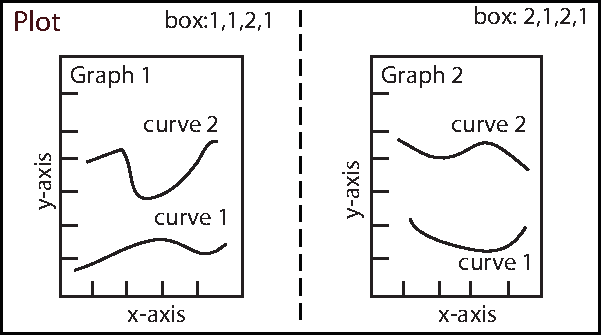
\includegraphics[width=5.0in]{plot-plot.pdf}
  \caption[Plotting nomenclature.]
  {
A plot has a collection of graphs and a graph has a collection of curves. A graph is located within
a plot by defining the ``\vn{box}'' associated with the \vn{graph}. Illustrated here is a plot with
two graphs placed side by side.
  }
  \label{f:plot.plot}
\end{figure}

%-----------------------------------------------------------------
\section{Box}
\label{s:box.def}

To determine where a \vn{graph} is drawn with respect to the boundaries of its associated \vn{plot},
each \vn{graph} is associated with a given ``\vn{box}''. A \vn{box} is a rectangular sub-region of
the \vn{plot}. Boxes are defined by dividing the \vn{plot} into a rectangular grid and then choosing
one of the grid rectangles to be the \vn{box} associated with the \vn{graph}. The is illustrated in
\fig{f:plot.plot} where \vn{Graph 1} is associated with the \vn{box} labeled ``\vn{1,1,2,1}'' and
\vn{Graph 2} is associated with the \vn{box} labeled \vn{2,1,2,1}.  The last two digits of a
\vn{box} label (\vn{2,1} for both graphs) specify the number of rectangles the grid has horizontally
and vertically (2 horizontally, 1 vertically here). The first two digits (\vn{1,1} for \vn{graph 1}
and \vn{2,1} for \vn{graph 2}) specify the particular rectangle associated with the \vn{box} with
\vn{1,1} designating the lower left rectangle. Different \vn{graphs} do not have to use the same
grid division to select a box from.

Setting the \vn{box} for a given \vn{graph} in a \tao initialization file is covered in \sref{s:template}.
The \vn{set graph} and \vn{show graph} commands can be used to set and show the box parameters. 
Examples:
\begin{example}
  set graph myplot.g1 box = 2 1 2 2  ! Set box of graph myplot.g1
  set graph myplot.g2 box = 1 1 1 2  ! Different graphs can use different grids
                                     !  for box selection
\end{example}

%-----------------------------------------------------------------
\section{Graph}
\label{s:graph.def}

%-----------------------------------------------------------------
\subsection{Overview}
\label{s:graph.overview}

A \vn{graph} is a diagram of some sort. Most \vn{graph}s consists of horizontal and vertical axes
along with one or more \vn{curve}s. \vn{Floor_plan} (\sref{s:floor.plan}) and \vn{lat_layout}
(\sref{s:lat.layout}) \vn{graphs}, on the other hand, shows the placement in space of the lattice
elements and do not have any associated \vn{curves}.

Every \vn{plot} has at least one \vn{graph}. How many \vn{graphs} are associated with a \vn{plot}
is a matter of convenience and different \vn{graphs} of a \vn{plot} may display different types of
information. For example, it would be possible to have a single \vn{plot} contain three \vn{graphs}
and look like what is shown in \fig{f:plot.typ}. In actuality, the figure was constructed using
three \vn{plots} each one containing one \vn{graph}.

How to define \vn{graphs} when defining \vn{template} plots is given in \sref{s:template}. The
\vn{show graph} command can be used to show graph parameters. The \vn{set graph} command can
be used to modify \vn{graph} parameters.

%-----------------------------------------------------------------
\subsection{Graph Name}
\label{s:graph.name}

All graphs have a name. For example, the graph of the standard \vn{orbit} plot is simply ``\vn{g}''.
\vn{Graphs} may be referred to using the syntax:
\begin{example}
  <plot>.<graph>
\end{example}
where \vn{<plot>} is the plot name (or the \vn{region} name associated with the \vn{plot}) and
\vn{<graph>} is the graph name. If the \vn{.<graph>} ending is omitted, all graphs of the named
\vn{plot}(s) are selected. Examples:
\begin{example}
  show graph beta   ! Show info of all graphs in all the displayed beta plots.
  show graph r13.g1 ! Show info on ``g1'' graph of region r13.
\end{example}

%-----------------------------------------------------------------
\subsection{Curve Legend of a Graph}
\label{s:curve.legend}

The \vn{curve legend} is the legend identifying what curves are associated with what perimeters. In
\fig{f:plot.typ} the top two graphs have a curve legend in the upper left hand corner of the graph.
By default, the \vn{data_type} of each curve will be used as the text for that
curve's line in the legend.  This default can be changed by setting a curve's \vn{curve%legend_tex}.
Parameters that affect the curve legend are:
\begin{example}
  plot_page%legend_text_scale        
  plot_page%curve_legend_line_len    ! tao_plot_page namelist (\sref{s:plot.page})
  plot_page%curve_legend_text_offset ! tao_plot_page namelist (\sref{s:plot.page})
  curve(N)%legend_text               ! 
  graph%curve_legend_origin          
  graph%draw_curve_legend            
\end{example}
The curve legend is distinct from the \vn{text legend} (\sref{s:text.legend}).

%-----------------------------------------------------------------
\subsection{Text Legend}
\label{s:text.legend}

The \vn{text legend} is a legend that can be setup by either the user or by \tao itself.
\tao uses the text legend in conjunction with phase space plotting or histogram displays.
The \vn{text legend} is distinct from the \vn{curve legend}. Parameters that affect the text
legend are:
\begin{example}
  graph%text_legend(N)
  graph%text_legend_origin
\end{example}

%-----------------------------------------------------------------
\subsection{Graph Types}
\label{s:graph.types}

\tao defines several kinds of graphs. The \vn{graph%type} in the \vn{tao_template_graph}
(\sref{s:template}) sets the type.
\begin{description}
%
\item["data"] \Newline
``Data'' plotting is the plotting of a dependent variable on the $y$-axis vs an independent variable
on the $x$-axis. Typically the independent variable will be the longitudinal position $s$-position
as in the upper two graphs in \fig{f:plot.typ}. Also see \Sref{s:draw.ap} for an example where beam
apertures are added to the graph.

A ``\vn{data slice}'' graph is plotting one data array on the $y$-axis versus another data array on
the $x$-axis (\sref{s:graph.data.slice}). Also see \vn{parametric plotting} (\sref{s:param.plot}).

With a \vn{parametric} plot both the $x$ and $y$ values of the points on a curve are dependent
upon an independent parameter (\sref{s:param.plot}). This is similar to a \vn{data slice} plot
(\sref{s:graph.data.slice}).
%
\item["dynamic_aperture"] \Newline
A \vn{dynamic aperture} graph (\sref{s:da.plot}) draws the results from a dynamic aperture
calculation (\sref{s:da.calc}).
%
\item["floor_plan"] \Newline
A \vn{floor plan} graph shows the physical layout of the machine (\sref{s:floor.plan}). A table maps
lattice elements to a shape that is drawn (\sref{s:shapes}). The user may override the default
mapping. Besides the lattice elements. the outline of the building or tunnel that the machine is in
can be drawn (\sref{s:building.wall}).
%
\item["histogram"] \Newline
Currently \vn{histograms} (\sref{s:histogram}) are limited to displaying phase space data.
%
\item["key_table"] \Newline
The \vn{key table} displays information about variables bound to keyboard keys \sref{s:key.bind}.
Key bindings are used in \vn{single mode}.
%
\item["lat_layout"] \Newline
A \vn{lattice layout} graph displays the lattice elements as a series of shapes as a function of the
longitudinal position $s$ (\sref{s:lat.layout}). The lowest graph in \fig{f:plot.typ} is an example
of a \vn{lattice layout}.  A table maps lattice elements to a shape that is drawn (\sref{s:shapes}).
The user may override the default mapping.
%
\item["phase_space"] \Newline
A \vn{phase space graph} (\sref{s:phase.space}) displays particle positions in phase space after
a beam of particles has been tracked (\sref{s:beam.init}).
%
\item["wave.0", "wave.a", "wave.b"] \Newline
Wave analysis plotting (\sref{c:wave}).
%
\end{description}

\begin{figure}[b]
  \centering
  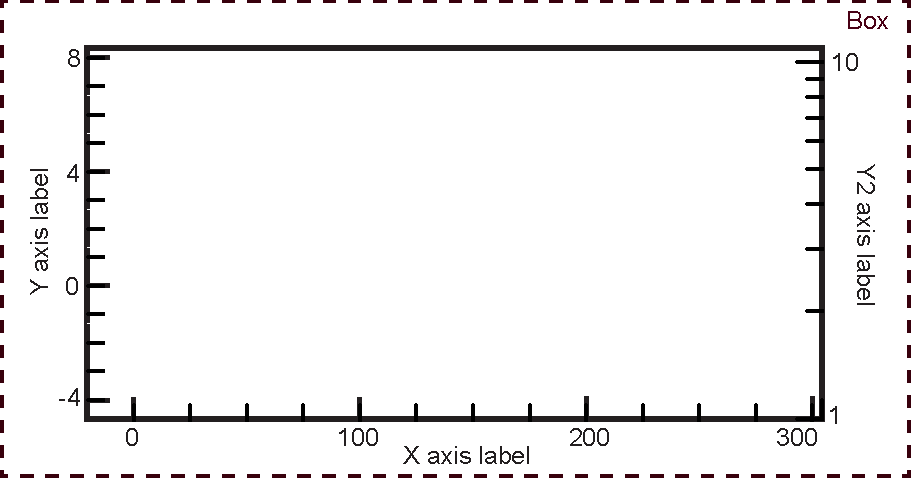
\includegraphics[width=5.0in]{plot-axes.pdf}
  \caption[Plot axes.]
{A data graph has three axes called \vn{x} (bottom edge), \vn{y} (left edge), and \vn{y2} (right edge).}
  \label{f:plot.axes}
\end{figure}

%-----------------------------------------------------------------
\subsection{Graph Axes}
\label{s:axes}

Data graphs (\sref{s:graph.types}) have three axes as shown in \fig{f:plot.axes}. The bottom axis is
called \vn{x}, and the left and right axes are called \vn{y} and \vn{y2} respectively. The \vn{qp_axis_struct}
structure (\sref{s:qp.axis}) is used to store axis parameters.

The \vn{scale} command (\sref{s:scale}) can be used to set the vertical axes. The \vn{x_scale}
(\sref{s:x.scale}) command can be used to set the horizontal axis.

Normally there is only one vertical scale for a graph and this is associated with the \vn{y}
axis. However, if any curve of a given graph has \vn{curve%use_y2} set to \vn{True} then the \vn{y2}
axis will have an independent second scale. In this case, the \vn{y2} axis numbers will be
drawn. Notice that simply giving the \vn{y2} axis a label does {\em not} make the \vn{y2} axis scale
independent of the \vn{y} axis scale.

%-----------------------------------------------------------------
\section{Curve}
\label{s:curve.def}

%-----------------------------------------------------------------
\subsection{Overview}
\label{s:curve.overview}

A \vn{curve} is a data set to be displayed within a \vn{graph}. For example, a \vn{curve} may be the
beta function of the \vn{model} lattice. \vn{Curves} have an associated set of points at which a
symbol can be drawn. A curve also can have an associated curved line that can be drawn. For example,
in \fig{f:plot.typ} only the line is drawn with the two curves of the beta plot while both symbols
and line are drawn for the two curves of the orbit plot (here the data points where symbols are
drawn are the orbit at the edges of the lattice elements).

Some \vn{graphs} do not have any associated curves. For example, a \vn{lat_layout} graph does not
have associated curves.

How to define \vn{curves} when defining \vn{template} plots is given in \sref{s:template}. The
\vn{show curve} command can be used to show curve parameters. The \vn{set curve} command can
be used to modify \vn{curve} parameters.

%-----------------------------------------------------------------
\subsection{Curve Name}
\label{s:curve.name}

All curves have a name. \vn{Curves} may be referred to using the syntax:
\begin{example}
  <plot>.<graph>.<curve>
\end{example}
where \vn{<plot>} is the plot (or \vn{region}) name, \vn{<graph>} is the graph name and \vn{<curve>}
is the curve name. If the \vn{.<curve>} ending is omitted, all curves of the named \vn{graph}(s) are
selected. If the \vn{.<graph>.<curve>} ending is omitted, all curves of the named \vn{plot}(s) are
selected. Examples:
\begin{example}
  show curve beta   ! Show info of all curves in all the displayed beta plots.
  show curve r13.g1 ! Show info on curves in ``g1'' graph of region r13.
  set graph orbit.g curve_legend_origin = 0.1 -0.2 "%BOX/LT"  ! Set curve legend origin
\end{example}
The last example sets the \vn{curve legend} (\sref{s:template}) of the graph so that the curve
legend of the graph is drawn with respect to the left top corner of the box.

%-----------------------------------------------------------------
\subsection{Curve Line}
\label{s:curve.line}

Each curve may have an associated line that is drawn. The line may be a set of line segments
connecting curve symbol points (\sref{s:curve.sym}) or may be a ``smooth'' curve calculated by
evaluating the curve at a number of points. 

\vn{curve%draw_line} determines whether a curve is drawn through the data point symbols. The
thickness, style (solid, dashed, etc.), and color of the line can be controlled by setting
\vn{curve%line}. If \vn{plot%x_axis_type} is \vn{"s"}, and \vn{curve%component} does not contain
\vn{"meas"} or \vn{"ref"}, \tao will attempt to calculate intermediate values in order to draw a
smooth, accurate curve is drawn. Occasionally, this process is too slow or not desired for other
reasons so setting \vn{curve%smooth_line_calc} to False will prevent this calculation and the curve
will be drawn as a series of lines connecting the symbol points. The default of
\vn{curve%smooth_line_calc} is True. Use the \vn{set curve} command (\sref{s:set}) to toggle the
drawing of lines. Alternatively, the \vn{-disable_smooth_line_calc} switch can be used on the
command line (\sref{s:command.line}) or the global variable \vn{global%disable_smooth_line_calc} can
be set in the \tao initialization file (\sref{s:globals}).

The number of points to evaluate at when constructing a smoothed line is set by
\vn{plot_page%n_curve_pts} in the \vn{tao_plot_page} namelist (\sref{s:plot.page}) or by using the
\vn{set plot_page} command (\sref{s:set.plot.page}). To override this value for a particular plot
the \vn{plot%n_curve_pts} parameter can be set in the \vn{tao_template_plot} namelist or using the
\vn{set plot} command (\sref{s:set.plot}). More evaluation points may give a more accurate curve at
the expense of computation time.

%-----------------------------------------------------------------
\subsection{Curve Symbol}
\label{s:curve.sym}

\vn{curve%draw_symbols} determines whether a symbol is drawn at the data points. The size, shape and
color of the symbols is determined by \vn{curve%symbol}. A given symbol point that is drawn has
three numbers attached to it: The $(x, y)$ position on the graph and an index number to help
identify it. The index number of a particular symbol is the index of the datum or variable
corresponding the symbol in the \vn{d1_data} or \vn{v1_var} array. These three numbers can be
printed using the \vn{show curve -symbol} command (\sref{s:show}).  \vn{curve%draw_symbol_index}
determines whether the index number is printed besides the symbol. Use the \vn{set curve} command
(\sref{s:set}) to toggle the drawing of symbols. The default value for \vn{curve%draw_symbol} is
False if \vn{plot%x_axis_type} is \vn{"s"}, \vn{"curve"}, \vn{"lat"}, or \vn{"var"} and True
otherwise. The default \vn{curve%draw_symbol_index} is always False.

The \vn{graph%draw_only_good_user_data_or_vars} logical determines whether datums
(\sref{s:init.data}) or variables (\sref{s:init.var}) with a \vn{good_user} component set to
\vn{False} are drawn. The default is to not draw them which means that data or variables not used in
an optimization are not drawn.

%-----------------------------------------------------------------
\subsection{Curve Component}
\label{s:curve.comp}

A ``\vn{data}'' graph (\sref{s:graph.types}) is used to draw lattice parameters such as orbits, or
\tao data (\sref{c:data}), or variable values such as quadrupole strengths. The data values will
depend upon where the data comes from. This is determined, in part, by the setting of the
\vn{component} parameter in the \vn{tao_template_graph} namelist (\sref{s:template}).  The
\vn{component} may be one of:
\index{model}\index{design}\index{base}\index{meas}\index{ref}
\begin{example}
  "model"             ! model values. Default.
  "design"            ! design values.
  "base"              ! Base values
  "meas"              ! data values.
  "ref"               ! reference data values.
  "beam_chamber_wall" ! Beam chamber wall
\end{example}
Additionally, \vn{component} may be set to plot a linear combination of the above. For
example:
\begin{example}
  &tao_template_graph
    curve(2)%component = "model - design"
    ...
\end{example}
This will plot the difference between the \vn{model} and \vn{design} values. 
The default value of \vn{%component} is \vn{"model"}.

%-----------------------------------------------------------------
\subsection{Curve Data Source}
\label{s:curve.source}

\index{data}\index{var}\index{calculation}
\index{curve!data_source}
The \vn{data_source} parameter of a curve is the type of information for the source of the data points.
\vn{data_source} must be one of:
\begin{example}
  "data"              ! A d1_data array is the source of the curve points.
  "var"               ! A v1_var array is the source of the curve points.
  "lat" (Default)     ! The curve points are computed directly from the lattice.
  "beam"              ! The curve points are computed from tracking a beam of particles.
  "multi_turn_orbit"  ! Computation is from multi-turn tracking. 
\end{example}
The default for \vn{data_source} is \vn{"lat"}. With \vn{data_source} set to "\vn{data}",
the values of the curve points come from the \vn{d1_data} array structure named by
the curve's \vn{data_type} parameter (\sref{s:curve.type}).

If \vn{data_source} is set to \vn{var}, the values of the curve points come from a \vn{v1_var}
array structure. If it is set to \vn{lat} the curve data points are calculated from the lattice
without regard to any data structures. \vn{data_source} can be set to \vn{beam} when tracking
beams of particles. In this case, the curve points are calculated from the tracking. With \vn{beam},
the particular bunch that the data is extracted from can be specified via \vn{ix_bunch}. The
default is \vn{0} which combines all the bunches of the beam for the calculation.

Used in conjunction with \vn{data_type} and \vn{component} (\sref{s:curve.comp}). For
example (\sref{s:curve.source}), a curve of the orbit with \vn{data_source} set to \vn{"beam"}
would use the beam centroid computations. If the \vn{data_source} was set to \vn{"lat"} the
computed orbit using single particle tracking is used.

Example: With \vn{data_type} set to \vn{beta.x}, the setting of \vn{data_source} to
\vn{lat} gives the beta as calculated from the lattice and \vn{beam} gives the beta as calculated
from the shape of the beam.

%-----------------------------------------------------------------
\subsection{Curve Data Type}
\label{s:curve.type}

The \vn{data_type} of a curve specifies what is being plotted. What the valid settings for \vn{data_type}
are depends upon the type of graph (\sref{s:graph.types}). 
\begin{description}
%
\item[graph\%type = "data", or "histogram"] \Newline
Valid settings for \vn{data_type} are any \tao datum type (\sref{s:data.table}), \tao variable
(\sref{c:var}), and the following electric and magnetic field components:
\begin{example}
  b0_field.x,  b0_field.y,  b0_field.z,  b0_curl.x,  b0_curl.y,  b0_curl.z,  b0_div
  e0_field.x,  e0_field.y,  e0_field.z,  e0_curl.x,  e0_curl.y,  e0_curl.z,  e0_div
\end{example}
The field data types with names starting with ``b_'' and ``e_'' evaluate the field along the single
particle trajectory while the field data types with names starting with ``b0_'' and ``e0_'' are evaluated
along a constant transverse position specified by the curve's \vn{orbit} parameter.
%
\item[graph\%type = "dynamic_aperture"] \Newline
Valid settings for \vn{data_type} are:
\begin{example}
  "beam_ellipse"
  "dynamic_aperture"
\end{example}
%
\item[graph\%type = floor_plan", "lat_layout", or "key_table"] \Newline
There are not curves associated with these graph types.
%
\item[graph\%type = "phase_space"] \Newline
Valid settings for \vn{data_type} are:
\begin{example}
  "x",  "px",  "y",  "py",  "z",  "pz",
  "intensity",  "intensity_x",  "intensity_y"     ! Photon intensity
  "phase_x", "phase_y"                            ! Photon coherent phase
\end{example}
%
\end{description}

 For example, with \vn{graph%type} set to
\vn{dynamic_aperture} the 




Thus in the above example the curve point values are obtained from
\vn{orbit.x} data. To be valid the data structure named by \vn{data_type} must be set up in an
initialization file. If not given, the default \vn{data_type} is
\begin{example}
  <plot%name>.<graph%name>
\end{example}

%-----------------------------------------------------------------
\section{Quick_Plot Plotting}
\label{s:quick.plot}

\vn{Quick_plot} is a software library developed for \bmad and \tao for graphics plotting.

%-----------------------------------------------------------------
\subsection{Length and Position Units}
\label{s:qp.units}

Positions and lengths with \vn{quick_plot} generally have an associated ``\vn{units}'' string which determines how
$(x, y)$ positions or $(dx, dy)$ lengths are to be interpreted. 
The syntax of the \vn{units} parameter is:
\begin{example}
  "unit_type/ref_object/corner"
\end{example}
A \vn{units} string has a \vn{unit_type}, \vn{ref_object} and \vn{corner} components separated by slashes ``/''.

The \vn{unit_type} component is the type of units which can be one of:
\begin{example}
   "%"       - Percent.
   "DATA"    - Data units associated with a graph.
   "MM"      - millimeters.
   "INCH"    - Inches.
   "POINTS"  - Printers points (72 points = 1 inch, 1 pt ~ 1 pixel).
\end{example}
Note: If \vn{unit_type} is set to \vn{"DATA"}, \vn{ref_object}, if present, must be \vn{"GRAPH"} and
\vn{corner}, if present, must be \vn{"LB"}.

The \vn{ref_object} component is a reference object which can be one of:
\begin{example}
   "PAGE"  -- Relative to the plot display window.
   "BOX"   -- Relative to the box the graph is associated with.
   "GRAPH" -- Relative to the graph rectangle.
\end{example}
The \vn{ref_object} component is optional if a relative length is being specified and the
\vn{unit_type} is anything other than \vn, the slash between
the \vn{unit_type} and the \vn{ref_object} may be omitted.

Note: The \vn{"PAGE"} reference is the entire \vn{plot page} and not the \vn{plot area}. The
\vn{plot area} is only used for defining the placement of \vn{regions}.

The \vn{corner} component is the origin location of the reference object.
\vn{corner} can be one of:
\begin{example}
   "LB" -- Left Bottom of reference object. Default.
   "LT" -- Left Top.
   "RB" -- Right Bottom.
   "RT" -- Right Top.
\end{example}
The \vn{ref_object} component is optional if a relative length is being specified.

Examples:
\begin{example}
  "DATA"          -- Equivalent to "DATA/GRAPH/LB"
  "DATA/GRAPH/LB" -- Same as above.
  "DATA/BOX/RT"   -- ILLEGAL: DATA must always go with GRAPH/LB.
  "%/PAGE/LT"     -- Equivalent to "%PAGE/LT"
  "%PAGE/LT"      -- Percentage of page so (0.0, 1.0) = RT of page.
  "%BOX"          -- Percentage of box so (1.0, 1.0) = RT of box.
  "INCH/PAGE"     -- Inches from LB of page. Equivalent to "INCH/PAGE/LB"
\end{example}

Units can be set in an initialization file or with the \vn{set} command. Example:
\begin{example}
  set plot_page title%units = '%PAGE'
\end{example}

%-----------------------------------------------------------------
\subsection{Text Justification Units}
\label{s:qp.str.just}

Text justification units is a two character string that sets where a line of text is to be printed
with respect to the text $(x, y)$ position.
The first character of the justification string gives the horizontal alignment:
\begin{example}
   "L" -- Left justify
   "C" -- Center justify
   "R" -- Right justify
\end{example}
The second character of the justification string gives the vertical alignment:
\begin{example}
   "B" -- Bottom justify
   "C" -- Center justify
   "T" -- Top justify
\end{example}

Example:
\begin{example}
  plot_page%title%justify = 'CC'
\end{example}

%-----------------------------------------------------------------
\subsection{qp_point_struct}
\label{s:qp.point}

\vn{QuickPlot} defines a number of structures to parameterize such things like line and symbol
properties.

The \vn{qp_point_struct} defines where a point is:
\begin{example}
  type qp_point_struct:
    x     = <real>     ! Horizontal offset of point from fiducial point
    y     = <real>     ! Vertical offset of point from fiducial point
    units = "<units>"  ! Units of x \& y (\sref{s:qp.units}).
\end{example}
Example:
\begin{example}
  graph%curve_legend_origin = 5.0, -2.0, "POINTS/GRAPH/LT"
\end{example}
In this example the fiducial point the left-top point on the graph rectangle. The
\vn{curve_legend_origin} is positioned 5.0 points horizontally to the left and 2.0 points vertically
downward from this fiducial point.

%-----------------------------------------------------------------
\subsection{qp_line_struct}
\label{s:qp.line}

The parameters associated with data lines drawn in a graph are contained in the \vn{qp_line_struct}:
\begin{example}
  type qp_line_struct:
    width    = <integer>  ! Default = 1
    color    = <string>   ! Default = "black" (\sref{s:qp.color}).
    pattern  = <string>   ! Default = "solid" (\sref{s:qp.line.pat}).
\end{example}

%-----------------------------------------------------------------
\subsection{Symbols}
\label{s:qp.sym}

The parameters associated with symbols that are drawn are contained in the \vn{qp_symbol_struct}:
\begin{example}
  type qp_symbol_struct:
    type          = <string>  ! Default = "dot"
    height        = <real>    ! Size in points. Default = 10
    color         = <string>  ! Default = "black" (\sref{s:qp.color})
    fill_pattern  = <string>  ! Default = "solid_fill"
    line_width    = <integer> ! Default = 1.
\end{example}

\begin{table}
  \centering
  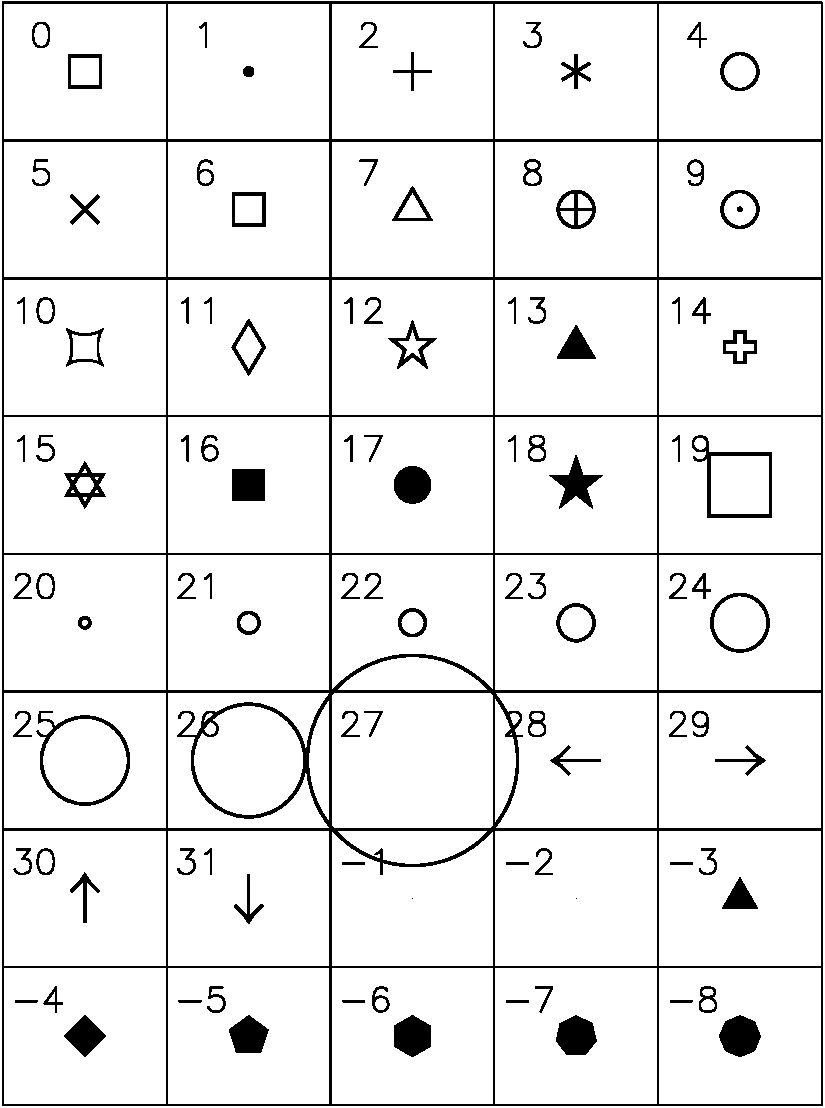
\includegraphics[width=5in]{plot-syms.pdf}
  \caption{Plotting Symbols.}
  \label{t:plot.syms}
\end{table}

The symbol types are:
\begin{example}
  square                 triangle                    square_concave              
  dot                    circle_plus                 diamond                     
  plus                   circle_dot                  star5                       
  times                  square_filled               triangle_filled           
  circle                 circle_filled               red_cross                 
  x                      star5_filled                star_of_david             
\end{example}
These symbols are illustrated in Table~\ref{t:plot.syms}. Symbol type names are case insensitive.

%-----------------------------------------------------------------
\subsection{qp_axis_struct}
\label{s:qp.axis}

The \vn{qp_axis_struct} structure defines the properties of a graph axis
\begin{example}
  type qp_axis_struct::
    label             = "<string>" ! Axis label string.
    min               = <real>     ! Min is the left or bottom axis number.
    max               = <real>     ! Max is the right or top axis number.
    number_offset     = <real>     ! Offset from axis line in inches.
    label_offset      = <real>     ! Offset from numbers in inches.
    major_tick_len    = <real>     ! Major tick length in inches.
    minor_tick_len    = <real>     ! Minor tick length in inches.
    label_color       = <string>   ! Color of the label string (\sref{s:qp.color})
    major_div         = <integer>  ! Number of major divisions
    major_div_nominal = <integer>  ! Major divisions nominal value.
    minor_div         = <integer>  ! Minor divisions. 0 = Tao will choose.
    minor_div_max     = <integer>  ! Max minor div number if Tao chooses.
    places            = <integer>  ! Number of digits to print
    type              = <string>   ! Axis type: "LINEAR" or "LOG".
    bounds            = <string>   ! Axis bounds: "GENERAL", "ZERO_AT_END", etc.
    tick_side         = <integer>  ! 1 = draw to the inside, 0 = both, -1 = outside.
    number_side       = <integer>  ! 1 = draw to the inside, -1 = outside.
    draw_label        = <logical>  ! Draw the label string
    draw_numbers      = <logical>  ! Draw the numbers.
\end{example}

The \vn{%bounds} parameter sets how the axes min and max values are calculated when plots are initially
instantiated and when \vn{scale}, \vn{x_scale}, and \vn{xy_scale} commands are used. Possible settings
are:
\begin{example}
  "ZERO_AT_END"      ! Min or max value is set to zero.
  "ZERO_SYMMETRIC"   ! Min and max chosen so that max = -min.
  "GENERAL"          ! No restrictions (default).
  "EXACT"            ! The User min/max is used.
\end{example}
If input min and max values are specified by the User, \tao will take the specified values as the starting
point to find ``nice'' min and max values to use. For example, with the command
\begin{example}
  scale all 0 19
\end{example}
and with \vn{bounds} set to \vn{"GENERAL"}, the min and max values will be set to 0 and 20. The exception is when
\vn{bounds} is set to \vn{"EXACT"}. In this case the User supplied min and max values will be used as is.

Examples:
\begin{example}
Tao> set graph r13 y%bounds = "zero_at_end"
Tao> scale r13 200 280   ! Graph bounds set to [0, 300]

Tao> set graph r13 y%bounds = "zero_symmetric"
Tao> scale r13 200 280   ! Graph bounds set to [-300, 300]

Tao> set graph r13 y%bounds = "general"
Tao> scale r13 20 190    ! Graph bounds set to [0, 200]

Tao> set graph r13 y2%bounds = "exact"
Tao> scale r13 -y2 20 190    ! Y2 graph bounds set to [20, 190]
\end{example}

Both \vn{major_div} and \vn{major_div_nominal} set the number of major divisions in the plot. The
difference between the two is that with \vn{major_div} set positive and \vn{major_div_nominal} set
zero or negative, the number of major divisions is fixed at the value of \vn{major_div}. With
\vn{major_div_nominal} positive, the value of \vn{major_div} is ignored, and the number of major
divisions will be chosen to be a ``nice'' value near the value of \vn{major_div_nominal}. If neither
\vn{major_div} nor \vn{major_div_nominal} is set positive, a value will be chosen for
\vn{major_div_nominal} by \tao. If you are unsure which to set, it is recommended that
\vn{major_div_nominal} be used.

The \vn{places} parameter set the number of places to display a number. \tao will automatically
calculate this number and it is not user settable.

The \vn{label} parameter may include Greek letters, subscripts, superscripts, and special characters.
Encoding for these are given in Table~\ref{t:plot.escape}. 


%-----------------------------------------------------------------
\subsection{String Escape Sequences}
\label{s:qp.str}

\begin{table}[tb]
\begin{tabular}{ll} \toprule
{\B}u       & Start a superscript or end a subscript \\[0.3ex]
{\B}d       & Start a subscript or end a superscript.
              {\B}u and {\B}d must always be used in pairs \\[0.3ex]
{\B}b       & Backspace (i.e., do not advance text pointer  
               after plotting the previous character) \\[0.3ex]
{\B}fn      & Switch to Normal font (1)       \\[0.3ex]
{\B}fr      & Switch to Roman font (2)        \\[0.3ex]
{\B}fi      & Switch to Italic font (3)       \\[0.3ex]
{\B}fs      & Switch to Script font (4)       \\[0.3ex]
{\B}{\B}    & Backslash character (\B)        \\[0.3ex]
{\B}x       & Multiplication sign ($\times$)  \\[0.3ex]
{\B}.       & Centered dot ($\cdot$)          \\[0.3ex]
{\B}A       & Angstrom symbol (\AA)         \\[0.3ex]
{\B}gx      & Greek letter corresponding to roman letter x. See Table~\ref{t:greek}. \\[0.3ex]
{\B}mN {\B}mNN & Graph marker number \vn{N} or \vn{NN} (1-31) \\[1ex]
{\B}(NNNN)  & 
\parbox{5.2in} {Character number NNNN (1 to 4 decimal digits) from the Hershey character set which
includes a number of special characters including mathematical, musical, astronomical, and
cartographical symbols.} \\ \bottomrule
\end{tabular}
\caption{Escape Sequences for Labels.}
\label{t:plot.escape}
\end{table}

Table~\ref{t:greek} shows how the character string \vn{"{\B}g<r>"}, where \vn{"<r>"} 
is a Roman letter, map onto the Greek character set.
\begin{table}[tb]
  \centering
  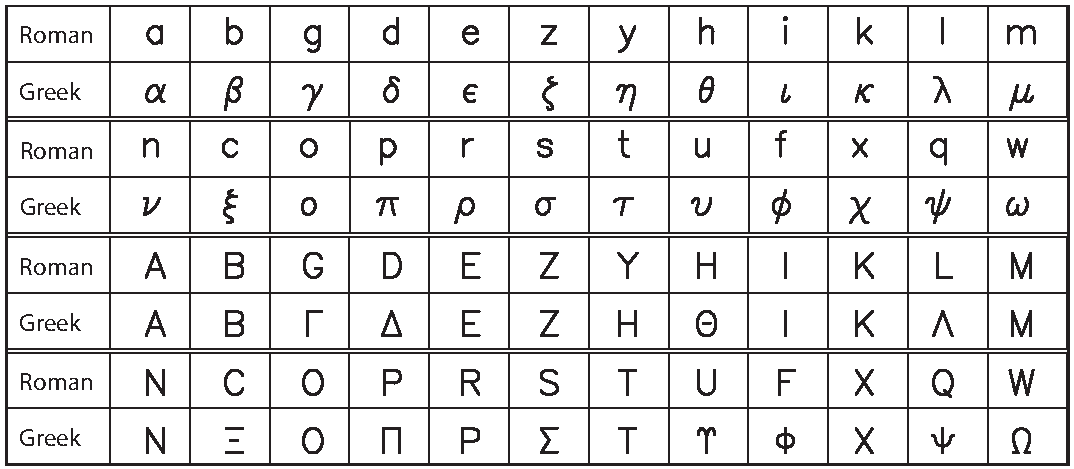
\includegraphics[width=5.0in]{greek.pdf}
  \caption[Roman to Greek Character Conversion]{Conversion for the string 
\vn{"{\B}g<r>"} where \vn{"<r>"} is a Roman character to the corresponding 
Greek character.}
\label{t:greek}
\end{table}

%-----------------------------------------------------------------
\subsection{Color Names}
\label{s:qp.color}

Possible settings for color parameters are:
\begin{example}
  White   (actually the background color)       Orange          
  Black   (actually the foreground color)       Yellow_Green    
  Red                                           Light_Green         
  Green                                         Navy_Blue       
  Blue                                          Purple          
  Cyan                                          Reddish_Purple  
  Magenta                                       Dark_Grey        
  Yellow                                        Light_Grey       
\end{example}
Color names are case insensitive.

%-----------------------------------------------------------------
\subsection{Line Pattern Names}
\label{s:qp.line.pat}

Possible settings for line patterns are:
\begin{example}
  solid      ! Solid line                 dotted     ! Dotted line             
  dashed     ! Dashed line                dash_dot3  ! Dash--dot--dot--dot line
  dash_dot   ! Dash--dot line
\end{example}
Pattern names are case insensitive.

%-----------------------------------------------------------------
\subsection{Fill Pattern Names}
\label{s:qp.fill.pat}

Possible fill pattern settings for symbols are:
\begin{example}
  solid_fill                    hatched           
  no_fill                       cross_hatched     
\end{example}
Fill pattern names are case insensitive.


\chapter{Optimization}
\label{c:opti}

%------------------------------------------------------------------------
\section{Lattice Corrections}

Examples of lattice corrections include flattening the orbit and
adjusting quadrupoles to correct the measured betatron phase. The
general idea is to vary an appropriate set of \vn{variables} with the
aim of minimizing a merit function \vn{M} that is a measure of how
well \vn{data_model}, the data as calculated from the \vn{model} fits
\vn{data_meas}, the measured data
\Begineq
  {\cal M} \equiv \sum_{i} w_i \,
    \bigl[ \data\_\model(i) -  \data\_\meas(i) \bigr]^2 + 
  \sum_{j} w_j \,
    \bigl[ \var\_\model(j) - \var\_\meas(j) \bigr]^2
  \label{m1}
\Endeq
\vn{var_model} is the value of a variable in the \vn{model} and
\vn{var_meas} is the value as measured at the time the data was taken
and the sum \vn{j} runs over all variables that are allowed to be
varied to minimize \vn{M}. The second term in the merit function
prevents degeneracies (or near degeneracies) in the problem which
would allow \tao to find solutions where \vn{data_model} matches
\vn{data_measured} with the \vn{var_model} having ``unphysical''
values (values far from \vn{var_meas}. The weights $w_i$ and $w_j$
need to be set depending upon how accurate the measred data is
relative to how accurate the calibrations for measuring the
\vn{var_meas} values are. With the second term in the merit function
the number of constraints (number of terms in the merit function) is
always larger than the number of variables and degeneracies can never
occur. 

The algorithm used to vary the \vn{var_model} variables to minimize
\vn{M} is called an \vn{optimizer}. In \vn{command line mode} the
\vn{run} command is used to invoke an \vn{optimizer}. In \vn{single
mode} the \vn{g} key starts an optimizer and the \vn{.} key stops it.
Running an optimizer is also called ``fitting'' since one is trying to
get the \vn{data_model} to be equal to the \vn{data_meas}. With orbits
this is also called ``flattening'' since one generally wants to end up
with an orbit that is on--axis.

In a correction one wants to change the machine variables so that the
measured data corresponds to the design values \vn{data_design}. Thus
the change in the data that one wants is
\begin{example}
  data_change = data_design - data_meas
\end{example}
Once a fit has been made, and presuming that the \vn{data_model} is
resonably close to the \vn{data_meas} this data change within the
\vn{model} lattice can be accomplished by changing the variables by
\begin{example}
  var_change = var_design - var_model
\end{example}
This assumes the system is linear. For many situations this is true
since typically \vn{var_change} is ``small''. Since the variables have
a measured value of \vn{var_meas} the value that the variables should
be set to is
\begin{example}
  var_final = var_meas + (var_design - var_model)
\end{example}
Notice that the fitting process is independent of the \vn{design}
lattice. It is only when calculating the corrections to the
variables that the \vn{design} lattice plays a roll. 

Sometimes it is desired to fit to changes in data as opposed to the
absolute value of the data. For example, when closing an orbit bump
knob what is important is the difference in orbits before and after
the bump knob is varied. Designating one of these orbit the
\vn{reference}, the appropriate merit function is
\begin{alignat}{1}
  {\cal M} = &\sum_{i} w_i \,
    \Bigl[ \bigl( \data\_\model(i) - \data\_\design(i) \bigr) - 
      \bigl( \data\_\meas(i) - \data\_\reference(i) \bigr) \Bigr]^2 + \CRNO
  &\sum_{j} w_j \,
    \Bigl[ \bigl( \var\_\model(j) - \var\_\design(j) \bigr) -
     \bigl( \var\_\meas(i) - \var\_\reference(i) \bigr) \Bigr]^2 
  \label{m2}
\end{alignat}
where \vn{data_ref} and \vn{var_ref} refer to the reference
measurement.  This merit function is acceptable if the reference data
is taken with the machine reasonably near the design setup so that
nonlinearities can be ignored. If this is not the case then the
fitting becomes a two step process: The first step is to fit the
\vn{model} to the \vn{reference} data using the merit function of
\Eq{m1}. The \vn{base} lattice is then set equal to the \vn{model}
lattice. The second step is to fit the model using the merit function
\begin{alignat}{1}
  {\cal M} = &\sum_{i} w_i 
    \Bigl[ \bigl( \data\_\model(i) - \data\_\base(i) \bigr) - 
      \bigl( \data\_\meas(i) - \data\_\reference(i) \bigr) \Bigr]^2 + \CRNO
  &\sum_{j} w_j 
    \Bigl[ \bigl( \var\_\model(j) - \var\_\base(j) \bigr) -
     \bigl( \var\_\meas(i) - \var\_\reference(i) \bigr) \Bigr]^2 
  \label{m3}
\end{alignat}

Control of what data and what variables are to be used in the fitting
process is controlled by the \vn{use}, \vn{veto}, \vn{restore}, and
\vn{clip} commands.

%------------------------------------------------------------------------
\section{Lattice Design}

Lattice design is the process of calculating \vn{variable} strengths
to meet a number of criteria called constraints. For example, one
constraint could be that the beta function in some part of the lattice
not exceed a certain value. In this case we can proceed as was done
for lattice correction and define a merit function to be minimized:
\Begineq
  {\cal M} = \sum_{i} w_i \, C_i^2
\Endeq
Typically constraints are either to limit values to some range so the
constraint would be of the form
\Begineq
  C = 
    \begin{cases}
    \mbox{model} - \mbox{limit}  & \mbox{model $>$ Limit} \\
    0                            & \mbox{otherwise}
    \end{cases}
\Endeq
or a constraint is used to keep the \vn{model} at a certain value so
the form of the constraint would be
\Begineq
  C = \mbox{model} - \mbox{target}  
\Endeq
Here \vn{model} is the value as calculated from the \vn{model}
lattice. \vn{target} and \vn{limit} are given numbers. Part of the
optimization process is in deciding what the values should be for any
\vn{target} or \vn{limit}.

%------------------------------------------------------------------------
\section{Generalized Design}

Since lattice design and lattice corrections are similar, \tao
combines the two into one generalized correction process. In this
generalized process The merit function becomes
\Begineq
  {\cal M} = \sum_i w_i \, D_i^2 + \sum_j w_j \, V_j^2
\Endeq
The general form of the data merit terms $D_i$ is 
\Begineq
  D = 
    \begin{cases}
    \mbox{delta}  & \mbox{Non-zero Condition} \\
    0             & \mbox{Otherwise}
    \end{cases}
\Endeq
The \vn{Non-zero Condition} needed for a non--zero $C_i$ is dependent
upon the \vn{merit_type} of the datum. There are five constraint
types as given in Table~\ref{t:con_type}.
\begin{table}[h]
\centering
{\tt
\begin{tabular}{|l|l|l|} \hline
  {\it Merit\_Type}       & {\it Non-zero Condition} \\ \hline 
  \vn{target}            & Any \vn{delta}   \\ \hline 
  \vn{min}, \vn{abs_min} & \vn{delta} $<$ 0 \\ \hline 
  \vn{max}, \vn{abs_max} & \vn{delta} $>$ 0 \\ \hline 
\end{tabular}
}
\caption{Constraint Type List.}
\label{t:con_type}
\end{table}

The form of \vn{delta} is determined by two global logicals called
\vn{opt_with_ref} and \vn{opt_with_base} as shown in
Table~\ref{t:d_i}. 
\begin{table}[h] 
\centering 
{\tt
\begin{tabular}{|l|l|l|} \hline
  \vn{Opt_with_ref} & \vn{Opt_with_base} & \vn{delta} \\ \hline 
  F & F & Model - Meas                \\ \hline 
  T & F & Model - Meas + Ref - Design \\ \hline 
  F & T & Model - Meas - Base         \\ \hline 
  T & T & Model - Meas + Ref - Base   \\ \hline 
\end{tabular}
} 
\caption{$D_i$ Form}  
\label{t:d_i}
\end{table}

What kind of data is associated with \vn{model}, \vn{design} and
\vn{base} is determined by a datum's \vn{data_type}. Valid
\vn{data_types} are given in table~\ref{t:cons}.
\begin{table}[h] 
\centering 
{\tt
\begin{tabular}{|l|l|l|} \hline
  {\it Data\_Type} & {\it Description}        &          \\ \hline 
    beta:x, beta:y    & Twiss parameter                 &          \\ \hline 
    alpha:x, alpha:y  & Twiss parameter                 &          \\ \hline 
    eta:x, eta:y      & Dispersion                      &          \\ \hline 
    etap:x, etap:y    & Dispersion derivative           &          \\ \hline 
    phase:x, phase:y  & Betatron phase                  & relative \\ \hline 
    orbit:x, orbit:y  & Particle orbit                  &          \\ \hline 
\begin{tabular}{@{}l}     cbar:11, cbar:12, \\ cbar:21, cbar:22 \end{tabular} 
                      & Coupling                        &          \\ \hline 
\begin{tabular}{@{}l}     coupling:11b, coupling:12a, \\ 
                          coupling:12b, coupling:22a \end{tabular} 
                      & Coupling                        &          \\ \hline 
    floor:x, floor:y, floor:z
                      & Global (``floor'') position     & relative \\ \hline 
    floor:theta       & Global (``floor'') angle        & relative \\ \hline 
    r56               & Term in linear transfer map     & relative \\ \hline 
    t566              & Term in 2nd order transfer map  & relative \\ \hline 
    i5a\_e6, i5b\_e6  & Normalized I5 radiation integral &          \\ \hline
    s\_position       & longitudinal length constraint  & relative \\ \hline 
    beam\_energy      & Beam energy                     &          \\ \hline
\end{tabular}
} 
\caption{Constraint List.}
\label{t:cons}
\end{table}

Also associated with a datum are one or two lattice elements called
\vn{ele} and \vn{ele2}. The \vn{data_types} are divided into two
categories: Those that are \vn{relative} and those who are not.  A
\vn{relative} \vn{data_type} means that the \vn{model} value for that
datum is determined by a difference between elements. For example, for
\vn{phase:x} the \vn{model} value is
\begin{example}
  model_value = \(\phi\sb{x}\)(ele2) - \(\phi\sb{x}\)(ele)
\end{example}
If there is no \vn{ele2} associated with a datum then the model value is
\begin{example}
  model_value = \(\phi\sb{x}\)(ele) - \(\phi\sb{x}\)(0)
\end{example}
where $\phi_x(0)$ is the phase at the 0\Th element (which is always 0).

For datums with \vn{non-relative} \vn{data_types} If there is also an
associated \vn{ele2} element then the \vn{model} value is dependent
upon the \vn{merit_type}. For example, with a \vn{beta:x} \vn{data_type} the
model value is determined by Table~\ref{t:eval}.
\begin{table}[h]
\centering
{\tt
\begin{tabular}{|l|l|l|} \hline
  {\it Merit\_Type}       & {\it Model Value} \\ \hline 
  \vn{min}     & $\min_{\mbox{ele} \le i \le \mbox{ele2}} \beta_x(i)$ \\ \hline 
  \vn{max}     & $\min_{\mbox{ele} \le i \le \mbox{ele2}} \beta_x(i)$ \\ \hline 
  \vn{abs_min} & $\min_{\mbox{ele} \le i \le \mbox{ele2}} |\beta_x(i)|$ \\ \hline 
  \vn{abs_max} & $\min_{\mbox{ele} \le i \le \mbox{ele2}} |\beta_x(i)|$ \\ \hline 
  \vn{target}  & {\it Error}   \\ \hline 
\end{tabular}
}
\caption{\vn{Model} evaluation.}
\label{t:eval}
\end{table}

The form of the variable terms $V_i$ is determined by its \vn{merit_type}.
For variables the merit types are:
\begin{example}
  target
  limit
\end{example}
A \vn{target} \vn{merit_type} for a variable is the same as for
datum. In this case \vn{model} is just the value of the variable.
A \vn{limit} \vn{merit_type} has the form
\Begineq
  V = 
    \begin{cases}
    \mbox{model} - \mbox{high\_lim}  & \mbox{model} > \mbox{high\_lim} \\
    \mbox{model} - \mbox{low\_lim}   & \mbox{model} < \mbox{low\_lim} \\
    0                               & \mbox{Otherwise}
    \end{cases}
\Endeq

Note: when doing lattice design \vn{opt_with_ref} and
\vn{opt_with_base} are both set to \vn{False} and the \vn{target} and
\vn{limit} values are identified with \vn{Meas}.




\chapter{Wave Analysis}
\label{c:wave}

%----------------------------------------------------------------
\section{General Description}
\label{s:wave.general}

A ``wave analysis'' is method for finding isolated ``kick errors'' in
a machine by analyzing the appropriate data. Types of data that can be
analyzed and the associated error type is shown in
Table~\ref{t:wave0}.  

The analysis works on difference quantities. For example, the
difference between measurement and theory or the difference between
two measurements, etc. Orbit and vertical dispersion measurements are the
exception here since an analysis of, say, just an orbit measurement can
be considered to be the difference between the measurement and a
perfectly flat (zero) orbit.

\begin{table}[h]
\centering{\tt
\begin{tabular}{|l|l|} \hline
  {\it Measurement Type}  & {\it Error Type}           \\ \hline
  Orbit                   & Steering errors            \\ \hline
  Betatron phase          & Quadrupolar errors         \\ \hline
  Beta function           & Quadrupolar errors         \\ \hline
  Coupling                & Skew quadrupolar errors    \\ \hline
  Dispersion              & Sextupole errors           \\ \hline
\end{tabular}}
\caption[Wave measurement types.]
{Types of measurements that can be used in a wave analysis and the 
types of errors that can be diagnosed.}
\label{t:wave0}
\end{table}

\begin{figure}[t]
  \centering
  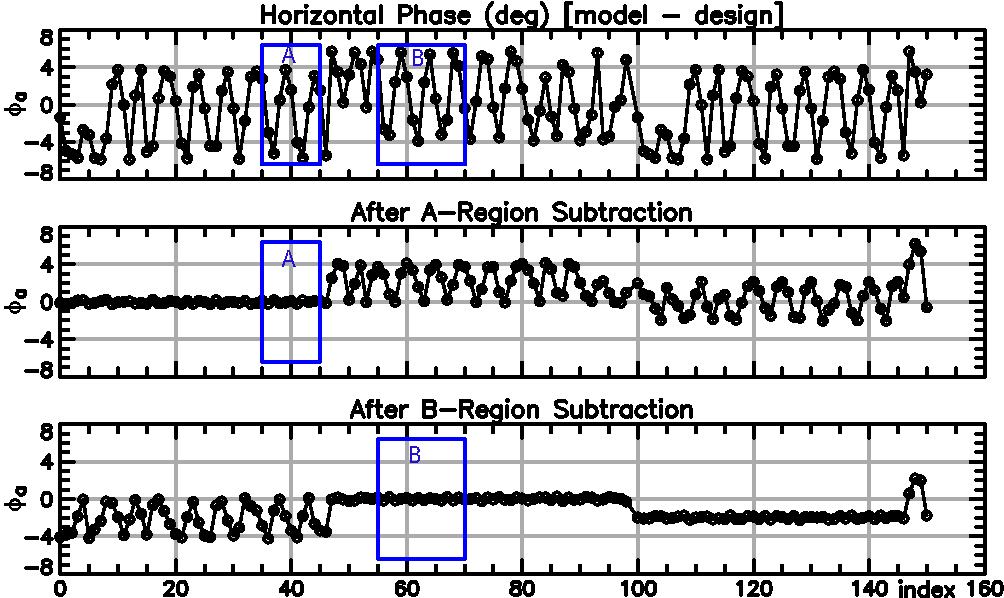
\includegraphics[width=6in]{wave.pdf}
  \caption[Example wave analysis.]
{Example wave analysis for betatron phase data.}
  \label{f:wave}
\end{figure}

The formulation of the wave analysis for quadrupolar and skew
quadrupolar errors is presented by Sagan\cite{b:wave}.  Although not
discussed in the paper, the wave analysis for orbit and dispersion
measurements is similar to the beta function analysis that is
presented. 

The wave analysis is similar for all the measurement types. How the
wave analysis works is illustrated in Figure~\ref{f:wave}.
Figure~\ref{f:wave}a shows the difference between \vn{model}
and \vn{design} values for the $a$-mode betatron phase for the Cornell's 
Cesr storage ring. In this example, one quadrupole in the model has 
been varied from it's design value. The horizontal axis is the detector index. 

For the wave analysis, two regions of the machine, labeled $A$ and $B$
in the figure, are chosen (more on this later). For each region in
turn, the data in that region is fit using a functional form that
assumes that there are no kick errors in the regions. 
For phase differences, this functional form is
\Begineq
  \delta phi(s) = D \, \sin(2 \, \phi(s) + phi_0) + C
  \label{xabps}
\Endeq
where $\phi$ is the phase
advance and the quantities $C$, $D$ and $\phi_0$ are varied to give the best
fit.  Once $C$, $D$, and $\phi_0$ are fixed, \Eq{xabps} can be evaluated at
any point. Figure~\ref{f:wave}b shows the orbit of \ref{f:wave}a
with the fit to the $A$ region subtracted off. Similarly,
Figure~\ref{f:wave}c shows the orbit of Figure~\ref{f:wave}a with
the fit to the $B$ region subtracted off. Concentrating on
Figure~\ref{f:wave}b, since there are no kick errors in the $A$
region, the fit is very good and hence the difference between the data
and the fit is nearly zero. Moving to the right from the $A$ region in
Figure~\ref{f:wave}b, this difference is nearly zero up to where the
assumption of no kick errors is violated. That is, at the location of
the quadrupole error  near detector 47. Similarly, since there are no kick errors
in region $B$, the difference between the data and the $B$ region fit
is nearly zero in Figure~\ref{f:wave}c and this remains true moving leftward
from region $B$ up to the quadrupole near detector 47.

By taking the fitted values for $C$, $D$, and $\phi_0$ for the regions $A$
and $B$, the point between the regions where the kick is generated and
the amplitude of the kick can be calculated. This calculation is
similar to that used to find quadrupolar errors from beta
data\ref{f:wave}. The one difference is a factor of 2 that appears
in the beta calculation due to the fact that a freely propagating beta
wave oscillates at $2\phi(s)$. 

The success of the wave analysis in finding a kick error depends upon
whether there are regions of sufficient size on both sides of the kick
that are kick error free. That is, whether the kick error is
``isolated''. The locations of the $A$ and $B$ regions are set by the
user and the general strategy is to try to find, by varying the
location of the regions, locations where the data is well fit within
the regions. The data is well fit if the difference between data and
fit is small compared to the data itself. If there are multiple
isolated kick errors, then each error in turn can be bracketed and
analyzed. If there are multiple errors so close together that they
cannot be resolved, this will throw off the analysis, but it may still
be possible to give bounds for the location where the kicks are at and
an ``effective'' kick amplitude can be calculated.

For circular machines, to be able to analyze kicks near the beginning
or end of the lattice, the wave analysis can be done by ``wrapping''
the data past the end of the lattice for another 1/2 turn. This is
illustrated in Figure~\ref{f:wave}. In the Cesr machine, there are
approximately 100 detectors labeled from 0 to 99.  The detectors from
100 to 150 are just the detectors from 0 to 50 shifted by 100. Thus,
for example, the detector labeled 132 in the figure is actually
detector 32.

%----------------------------------------------------------------
\section{Wave Analysis in Tao}
\label{s:wave.tao}

Performing a wave analysis in \tao is a three step process:
\begin{example}
  1) Plot the data to be analyzed.
  2) Use the \vn{wave} command to select the data.
  3) Use the \vn{set wave} command to vary the fit regions.
\end{example}

In general, the accuracy of the wave analysis depends upon the
accuracy with which the beta function and phase advances are known in
the baseline lattice used. \tao uses the \vn{model} lattice for the
baseline. If possible, One strategy to improve the accuracy of the
wave analysis is first use a measurement to calculate what the
quadrupole strengths in the \vn{model} lattice should be. Possible
measurements that can give this information include an orbit response
matrix (ORM) analysis, fits to beta or betatron phase measurements, etc.

%----------------------------------------------------------------
\subsection{Preparing the Data} 
\label{ss:wave.data}

At present (due to limited manpower to do the
coding), the wave analysis is restricted to data that is stored in a
\vn{d1_data} array (\sref{c:data}). That is, the plotted curve to be
analyzed must have its \vn{data_type} parameter set to
\vn{``data''} (\sref{s:init.data}). The possible data types that
can be analyzed are:
\begin{example}
  orbit.x, orbit.y
  beta.a,  beta.b
  phase.a, phase.b
  eta.x, eta.y
  cbar.11, cbar.12, cbar.21      ! Analysis not possible for cbar.21
  ping_a.amp_x, ping_a.phase_x
  ping_a.sin_y, ping_a.cos_y
  ping_b.amp_y, ping_b.phase_y
  ping_b.sin_x, ping_b.cos_x
\end{example}
The curve to be analyzed must be visible. Any combination of data
components may be used:. "meas", "meas-ref", "model", etc.

If data from a circular machine is being analyzed, the data is wrapped
past the end of the lattice for another 1/2 turn. The translation from
the data index in the wrapped section to the first 1/2 section of the
lattice is determined by the values of \vn{ix_min_data} and
\vn{ix_max_data} of the \vn{d1_data} array under consideration
(\sref{s:init.data}):
\begin{example}
  index_wrap \(\longrightarrow\) index_wrap - (ix_max_data - ix_min_data + 1)
\end{example}
For example, for the Cesr example in the previous section,
\vn{ix_min_data} was 0 and \vn{ix_max_data} was 99 to the translation
was
\begin{example}
  index_wrap \(\longrightarrow\) index_wrap - 100
\end{example}

%----------------------------------------------------------------
\subsection{Wave Analysis Commands and Output}
\label{ss:wave.cmd.out}

The \vn{wave} command (\sref{s:wave}) sets which plotted data curve
is used for the wave analysis. The \vn{set wave} command (\sref{s:set}) 
is used for setting the $A$ and $B$ region locations. Finally the 
\vn{show wave} command (\sref{s:show}) prints analysis results. 

Example wave analysis output with \vn{show wave}:
\begin{example}
  ix_a:  35  45
  ix_b:  55  70
  A Region Sigma_Fit/Amp_Fit:     0.018
  B Region Sigma_Fit/Amp_Fit:     0.015
  Sigma_Kick/Kick:    0.013
  Sigma_phi:          0.019
  Chi_C:              0.037 [Figure of Merit]

  Normalized Kick = k * l * beta [dimensionless]
     where k = quadrupole gradient [rad/m^2].
  After Dat#     Norm_K       phi
         46      0.0705    30.431
         49      0.0705    33.573
         53      0.0705    36.715
\end{example}
This output is for analysis of betatron phase data but the output for
other types of data is similar.  The first two lines of the output
show where the $A$ and $B$ regions are. The next two lines show
$\sigma_{a}/A_a$ and $\sigma_{b}/A_b$ where $\sigma_a$ and $\sigma_b$
are given by Eq.~(42) of Sagan\cite{b:wave} and 
\Begineq
  A_a \equiv \sqrt{\xi_a^2 + \eta_a^2}
\Endeq
with a similar equation for $A_b$. $\sigma_{a}/A_a$ and
$\sigma_{b}/A_b$ are thus a measure of how well the data is fit in the
$A$ and $B$ regions with a value of zero being a perfect fit and a
value of one indicating a poor fit. Notice that a poor fit of one of
the regions may simply be a reflection that the wave amplitude being
there. The next three lines of the output are $\sigma_{\delta
k}/\delta k$, $\sigma_\phi$, and $\xi_C$, and are given by Eq.~(39),
(43), and (44) respectively of \cite{b:wave}. The last three lines of
the analysis tell where the wave analysis predicts the kicks are and
what the normalized kick amplitudes are. Thus the first of these three
lines indicates that the kick may be somewhere after the location of
datum \#46 (but before the location of datum \#47), The normalized
quadrupole kick amplitude is 0.0705, and the betatron phase at the
putative kick is 30.431 radians.

\chapter{Tao Initialization}
\index{Initialization}
\label{c:init}

\tao is customized for specific machines and specific calculations using input files and custom
software routines. Writing custom software is covered in the programmer's guide section. This
chapter covers the input files.

In general, the input files tell \tao:
\begin{example}
  * What \bmad lattice or lattices to use (\sref{s:init.lat}).
  * What the variables and data should be when running optimizations (\sref{c:opti}).
  * What to plot and how plots should be laid out in the plotting window (\sref{s:init.plot}).
  * What kind of calculations are to be done. EG: a dynamic aperture calculation, etc.
  * Etc.
\end{example}

Example initialization files can be found in the \tao distribution in sub-directories of the
directory:
\begin{example}
  tao/examples
\end{example}

%-----------------------------------------------------------------
\section{Command Line Initialization}
\index{command line}
\label{s:command.line} 

The syntax of the command line for running \tao is:
\begin{example}
  EXE-DIRECTORY/tao \{OPTIONS\}
\end{example}
where \vn{EXE-DIRECTORY} is the directory where the tao executable lives. If this directory is
listed in your \vn{PATH} environmental variable then the directory specification may be omitted.
The optional arguments are:
\begin{description}
%
\item[\vn{-beam_file <file_name>}] \Newline
Sets the name of the file containing the \vn{tao_beam_init} namelist (\sref{s:beam.init}).
Overrides the setting of \vn{beam_file} (\sref{s:init.global}) specified in the \tao initialization
file.
%
\item[\vn{-beam_track_data_file <file_name>}] \Newline
Overrides the setting of \vn{beam_track_data_file} (\sref{s:beam.init}) specified in the \vn{tao_beam_init} namelist.
%
\item[\vn{-beam_init_position_file <file_name>}] \Newline
Specifies the file containing initial particle positions.  Overrides the setting of
\vn{beam_init%position_file} (\sref{s:beam.init}) specified in the \vn{tao_beam_init} namelist.
%
\item[\vn{-building_wall_file <file_name>}] \Newline
Overrides the \vn{building_wall_file} (\sref{s:init.global}) specified in the \tao initialization
file.
%
\item[\vn{-command <command_list>}] \Newline
List of commands to run at startup. This will be in addition to the commands run by the startup file
(\sref{s:init.global}). The startup file commands will be run before the commands specified by
\vn{-command}. Put the \vn{<command_list>} in quotes in order to embed blanks or if semicolons are
used to separate multiple commands. The \vn{-command} option is useful when running \tao from a
script. Example:
\begin{example}
  tao -command "show lat 12:14; quit"
\end{example}
In this example \tao will print some information on lattice elements 12 through 14 and then quit. The
output of the \vn{show} command can be captured by a script and processed.
%
\item[\vn{-data_file <file_name>}] \Newline
Overrides the \vn{data_file} (\sref{s:init.global}) specified in the \tao initialization file.
%
\item[\vn{-disable_smooth_line_calc}] \Newline
Disable computation of the ``smooth curves'' used in plotting.  This can be used to speed up \tao as
discussed in \sref{s:plot.data}.
%
\item[\vn{-external_plotting}] \Newline
This tells \tao that plotting is done externally to \tao. This is done, for example, when using a
Graphics User Interface (GUI) (\sref{s:gui.plot}).
%
\item[\vn{-geometry <width>x<height>}] \Newline
Overrides the plot window geometry. \vn{<width>} and \vn{<height>} are in Points. This is equivalent
to setting \vn{plot_page%size} in the \vn{tao_plot_page} namelist \sref{s:init.plot}.
%
\item[\vn{-hook_init_file}] \Newline
Specifies an input file for customized versions of Tao. Default file
name is \vn{tao_hook.init}.
%
\item[\vn{-init_file <file_name>}] \Newline
Replaces the default \tao initialization file name (\vn{tao.init}). Note: A \tao initialization file
is actually not needed. If no \tao initialization file is used, the use of the \vn{-lattice_file}
switch is mandatory and \tao will use a set of default plot templates for plotting.
%
\item[\vn{-lattice_file <file_name>}] \Newline
Overrides the \vn{design_lattice} lattice file specified in the \tao initialization file
(\sref{s:init.lat}). Example:
\begin{example}
  tao -init my.init -lat slac.bmad
\end{example}
If there is more than one universe and the universes have different lattices, separate the different
lattice names using a "|" character.  Do not put any spaces in between. Example:
\begin{example}
  tao -lat slac.bmad|cesr.bmad
\end{example}
%
\item[\vn{-log_startup}]
If there is a problem with starting \tao, \vn{-log_startup} can be used to create a log file of the
initialization process.
%
\item[\vn{-no_stopping}] \Newline
For debugging purposes. Prevents \tao from stopping where there is a fatal error.
%
\item[\vn{-noinit}] \Newline
Suppresses use of a \tao initialization file. In this case the use of the \vn{-lattice_file} switch
is mandatory and \tao will use a set of default plot templates for plotting.
%
\item[\vn{-noplot}] \Newline
Suppresses the opening of the plot window.
%
\item[\vn{-no_rad_int}] \Newline
Suppresses the radiation integrals calculation. Radiation integrals are used to calculate such
things as emittances, etc. Generally the calculation is not a problem but in some special
circumstances the calculation can take appreciable time.
%
\item[\vn{-plot_file <file_name>}] \Newline
Overrides the \vn{plot_file} (\sref{s:init.global}) specified in the \tao initialization file.
%
\item[\vn{-prompt_color}] \Newline
Sets the prompt string color to Blue. For different colors, use the \vn{set global prompt_color}
command (\sref{s:set}).
%
\item[\vn{-rf_on}]
Leaves \vn{rfcavity} elements on. Normally \tao turns off these elements since Twiss and dispersion
calculations do not make sense with them on.  Note: If you want to see orbit changes with RF
frequency changes then you will need to set \vn{parameter[absolute_time_tracking]} to True. See the
``Relative Versus Absolute Time Tracking'' section in the\bmad manual for more details.
%
\item[\vn{-slice_lattice <element_list>}]
If present, discard from the lattice all lattice elements that are not in the \vn{<element_list>}.
Overrides the setting of \vn{design_lattice(i)%slice_lattice}.
%
\item[\vn{-startup_file <file_name>}]
Overrides the \vn{startup_file} (\sref{s:init.global}) specified in the
\tao initialization file.
%
\item[\vn{-var_file <file_name>}] \Newline
Overrides the \vn{var_file} (\sref{s:init.global}) specified in the
\tao initialization file.

\end{description}

To negate an argument, use a two dash prefix instead of a single dash prefix. For example:
\begin{example}
  tao -noplot --noplot
\end{example}
The \vn{-noplot} argument turns off plotting and the following \vn{--noplot} argument negates the
effect of \vn{-noplot} and turns plotting back on. This is useful with the \vn{reinit tao} command
(\sref{s:reinit}) to negate saved command line argument settings.

%-----------------------------------------------------------------
\section{Namelist Syntax}
\label{s:format}

Parameters are read in from an initialization file using Fortran namelist input. Fortran namelist
breaks up the input file into blocks. The first line of a namelist block starts with an ampersand
``\&'' followed by the block identifying name. Variables are assigned using an equal sign ``='' and
the end of the block is denoted by a slash ``/'' For example:
\begin{example}
  &namelist_block_name
    var1 = 0.123   ! exclamation marks are used for comments
    var2 = 0.456
  /
\end{example}
Variables that have default values can be omitted from the block.  The order of the variables inside
a block is irrelevant except if the same variable appears twice in which case the last occurrence is
determinative.  In between namelist blocks all text is ignored. Inside a block comments may be
included by using an exclamation mark ``!''.

Care must be taken when setting arrays in a namelist as the following example shows:
\begin{example}
  &some_namelist_name
    var_array(8:11) = 34             ! Only sets var_array(8)
    var_array(8:11) = 34 34 81 81    ! OK. Sets all 4 values
    var_array(8:11) = 34, 34, 81, 81 ! OK. Same as above
    var_array(8:11) = 34, 34,        ! Lines may be continued ...
                      81, 81         !   ... like this.
    var_array(8:11) = 2*34 2*81      ! Equivalent to the preceding examples
    var_array(8:)   = 2*34 2*81      ! Also equivalent
    var_array(1:2) = 1 2 3           ! Error: Too many RHS values.
    string_arr = '1st' "2nd" '3rd'   ! Setting a string array.
    string_arr(1:3) = 1st 2nd 3rd    ! Same as above. [Not accepted by all compilers.]
    string_arr(1:3) = 1st,2nd,3rd    ! Same as above. [Not accepted by all compilers.]
    string_arr = 'A B' "2/" "&"      ! Quotes needed here.
  /
\end{example}
The first line to set the \vn{var_array} may look like it is setting the four values
\vn{var_array(8:11)} but the general rule is that with \vn{n} values on the RHS, only \vn{n} values
in the array are set.

{\em IMPORTANT:} The notation \vn{n*number} does not denote multiplication but instead can be used to
denote multiple values. There should be no blank spaces here. Some compilers may accept something
like ``2 * 34'' but you cannot count on it. Using ``2*34'' is safe. Also the gfortran compiler has a known
repeat count bug.

For string input it is always best to use quotes. Some compilers will accept strings without
quotes. Even those that do will generally not accept strings with special characters.  Thus the
following characters should not be used in unquoted strings:
\begin{example}
  Blank or Tab character.
  Period if it is the first character in the string.
  &   ,   /    !   %   *   (   )   =   ?   '   "
\end{example}
Note: While there are exceptions, in general \tao string variables are
case sensitive.

{\em WARNING:} Namelists cannot do expression evaluation. Thus the following will not work
\begin{example}
  &some_namelist_name
    a = 3.7/148
    b = 5
  /
\end{example}
The slash in the intended expression ``3.7/148'' will be taken as the namelist terminator. This
will result in variable \vn{a} having the value 3.7 and the value of variable \vn{b} will not
be set!

{\em WARNING:} Currently there is a bug in the gcc/gfortran compiler up to version 9 (GCC Bugzilla
\#82086) where repeat counts used with structure components cause \tao to halt with an error
message. For example:
\begin{example}
  &tao_template_graph
    curve(1:3)%y_axis_scale_factor = 3*1e3  ! Will not work with gfortran!!!
  /
\end{example}
Here \vn{curve} is a structure and \vn{y_axis_scale_factor} is a component of that structure. The
work around here is to eliminate the repeat count:
\begin{example}
  &tao_template_graph
    curve(1:3)%y_axis_scale_factor = 1e3, 1e3, 1e3
  /
\end{example}

Logical variables should be set to \vn{T} or \vn{TRUE} when true and \vn{F} or \vn{FALSE} when
false. This is case insensitive. It is possible to use the words \vn{.true.} and \vn{.false.} for
logicals, however this may not always work. The reason for this is that a variable that is
documented to be a logical may actually be a string variable! In this case a beginning period will
cause problems. Why use string variables? String variables are used in place of logical variables
when \tao needs to know if the variable has been explicitly set.

When setting an array in a namelist where the array components are a structure, the set can be
structured in several ways. To make this clear, consider the \vn{ele_shape(:)} array that can be set
in the \vn{lat_layout_drawing} namelist as explained in \sref{s:shapes}. Each component
of the \vn{ele_shape(:)} array is a structure and the elements of this structure are:
\begin{example}
  ele_shape(i) = "<ele_id>" "<shape>" "<color>" "<size>" "<label>" <draw> <multi> <line_width>
\end{example}
Setting a given \vn{ele_shape(:)} array component looks like:
\begin{example}
  &lat_layout_drawing
    !               ele_id                  Shape      Color     Size  Label  ..etc..
    ele_shape(2) = "quadrupole::*"          "xbox"     "red"     0.75  "none" 
  /
\end{example}
This sets the \vn{ele_id} component of \vn{ele_shape(2)} to \vn{"quadrupole::*"}, etc.

Alternatively, a given structure component can be set for multipole array components. Example:
\begin{example}
  &lat_layout_drawing
    ele_shape(5:6)%line_width = 5, 6
    ele_shape(3)%multi = T
  /
\end{example}
Here the \vn{line_width} structure component for \vn{ele_shape(5)} and \vn{ele_shape(6)} is set along
with the \vn{multi} structure component for \vn{ele_shape(3)}.

%-----------------------------------------------------------------
\section{Beginning Initialization}
\index{Initialization!beginning}
\label{s:init.global} 

\index{tao_start}\index{tao.init}\index{lattice_file}
\index{data_file}\index{var_file}\index{plot_file}
\index{single_mode_file}\index{startup_file}\index{startup_single_mode}
\index{beam_file}\index{hook_init_file}
The initialization starts with the \vn{root} \tao initialization file. The default name for this
file is \vn{tao.init} but this default may be overridden when \tao is started using the \vn{-init_file}
switch (\sref{s:command.line}). The first namelist block read in from the root initialization file is a
\vn{tao_start} namelist. This block is optional (in which case the defaults are used).  This
namelist contains the variables:
\begin{example}
  &tao_start
    beam_file          = "<file_name>"  ! Default = Tao root init file.
    building_wall_file = "<file_name>"  ! No Default.
    data_file          = "<file_name>"  ! Default = Tao root init file.
    var_file           = "<file_name>"  ! Default = Tao root init file.
    plot_file          = "<file_name1> \{<file_name2>\} ..."  
                                        ! Default = Tao root init file.
    single_mode_file   = "<file_name>"  ! Default = Tao root init file.
    startup_file       = "<file_name>"  ! Default = "tao.startup"
    hook_init_file     = "<file_name>"  ! Default = "tao_hook.init"
    init_name          = "<init_name>"  ! Default = "Tao"
  /
\end{example}
Rule: A file name obtained from the \tao root initialization file (as opposed to being present on
the command line) is always relative to the directory that the \tao root initialization file lives
in. Example: If \tao is started from the system command line like:
\begin{example}
    tao -data data.cl -init ../tao.init
\end{example}
And if the \vn{tao_start} namelist in \vn{../tao.init} looks like:
\begin{example}
  &tao_start
    data_file = "dat.in"
    plot_file = "plot.in"
    var_file  = "/nfs/var.in"
  /
\end{example}
Then, relative to the current working directory, the files used will be
\begin{example}
  data_file: "data.cl"      ! Command line arguments have preference
  plot_file: "../plot.in"   ! Relative to ../tao.init.
  var_file:  "/nfs/var.in"  ! Absolute paths are never modified.
\end{example}

\vn{init_name} is for naming the initialization. This is useful to distinguish between multiple
initialization files with custom versions of \tao. The other parameters specify which files to find
the other initialization namelists. The \vn{plot_file} variable can be an array of plot files.

\tao will open an execute a command file (\sref{s:command.files}) at startup if it exists.  The
default name is \vn{tao.startup} but this name can be changed by setting the \vn{startup_file}
component in the \vn{tao_start} namelist.

The following sections describe each of these initialization namelists and their locations are
listed in table~\ref{t:init.files}. Note: If \vn{plot_file} specifies multiple files, the
\vn{tao_plot_page}, \vn{lat_layout_drawing} and \vn{floor_plan_drawing} namelists are taken from the
first file on the list. All files, however, can contain \vn{tao_template_plot} and
\vn{tao_template_graph} namelists.

\index{tao_design_lattice}\index{tao_params}
\index{tao_beam_init}\index{tao_var}\index{tao_d2_data}
\index{tao_d1_data}\index{tao_plot_page}\index{tao_template_plot}
\index{tao_template_graph}\index{lat_layout_drawing}
\index{floor_plan_drawing}
\begin{table}[ht]
\centering {\tt
\begin{tabular}{llll} \toprule
  {\it Namelist}                     & {\it Type of Parameters Initialized}  & {\it Section} \\ \midrule
  \vn{lat_layout_drawing}            & Plotting           & \sref{s:shapes}            \\ 
  \vn{floor_plan_drawing}            & Plotting           & \sref{s:shapes}            \\ 
  \vn{tao_beam_init}                 & Particle beams     & \sref{s:beam.init}         \\ 
  \vn{building_wall_section}         & Building Walls     & \sref{s:building.wall}     \\ 
  \vn{symbolic_number}               & Symbolic Number    & \sref{s:init.sym}          \\
  \vn{tao_design_lattice}            & Lattice Files      & \sref{s:init.lat}          \\ 
  \vn{tao_d1_data}                   & Data               & \sref{s:init.data}         \\ 
  \vn{tao_d2_data}                   & Data               & \sref{s:init.data}         \\ 
  \vn{tao_dynamic_aperture}          & Dynamic Aperture   & \sref{s:dynamicaperture}   \\
  \vn{tao_params}                    & Global Parameters  & \sref{s:globals}           \\ 
  \vn{tao_plot_page}                 & Plotting           & \sref{s:init.plot}         \\ 
  \vn{tao_template_graph}            & Plotting           & \sref{s:init.plot}         \\ 
  \vn{tao_template_plot}             & Plotting           & \sref{s:init.plot}         \\ 
  \vn{tao_var}                       & Variables          & \sref{s:init.var}          \\ \bottomrule
\end{tabular}}
\break
\caption{Table of \vn{tao} Initialization Namelists.}
\label{t:init.files}
\end{table}

%-----------------------------------------------------------------
\section{Lattice Initialization}\index{initialization!lattice}
\label{s:init.lat} 

In the \vn{tao_start} namelist (\sref{s:init.global}), the \vn{lattice_file} variable gives the name
of the file that contains the \vn{tao_design_lattice} namelist. The default, if \vn{lattice_file} is
not present is to look in the \tao root initialization file. The \vn{tao_design_lattice} namelist
defines where the lattice input files are. The variables that are set in the \vn{tao_design_lattice}
namelist are:
\index{tao_design_lattice}\index{design_lattice}\index{design_lattice!file}
\index{design_lattice!parser}\index{n_universes}\index{common_lattice}
\begin{example}
  &tao_design_lattice
    n_universes        = <integer>      ! Number of universes. Default = 1.
    unique_name_suffix = "<string>"
    combine_consecutive_elements_of_like_name = <logical>
    common_lattice = <logical>                        ! Default = False
    design_lattice(i) = "<lattice_file>", \{"<lattice2_file>"\}
    design_lattice(i)%one_turn_map_calc = <logical>     ! Default = False
    design_lattice(i)%dynamic_aperture_calc = <logical> ! Default = False
    design_lattice(i)%reverse_lattice = <logical>      ! Default = False
    design_lattice(i)%slice_lattice = "<element_list>"             
  /
\end{example}

\vn{n_universes} is the number of universes to be created not counting the possible common universe
created when using \vn{CRL} analysis. The default is 1.  \vn{design_lattice(i)} gives the lattice
file name for universe \vn{i}.  The syntax for \vn{<lattice_file>} is:
\begin{example}
  \{<parser>::\}<lattice_file>\{@<use_line>\}
\end{example}
Possible choices for the <parser> are:
\index{bmad}\index{digested}
\begin{example}
  bmad      ! For a standard bmad lattice file. This is the default.
  digested  ! For a digested BMAD file.
\end{example}
The \vn{@<use_line>} optional suffix is used to specify what \vn{line} in the lattice file to use as
a basis for constructing the lattice. This overrides the \vn{use} statement in the lattice file.
Note: If the \vn{lattice_file} parameter is not set for the N\Th universe, the parameters for the 
previous universe are used.

If the \vn{%reverse_lattice} logical is present, the lattice will be reversed. That is, the elements
will be in reversed order. The sign of the charge of the tracked particle will be reversed for
proper tracking. This is useful for simulating beams that go in the backward direction. Note: If there
are any electric fields, the orbit in the reversed lattice will not be the reverse of the trajectory
in the unreversed lattice. Currently, lattice reversal only works if the lattice has a single branch.

The \vn{%slice_lattice} parameter specifies a list of elements to be used to pare down the lattice
so that the only elements that appear in the list are kept in the lattice.  In addition, any lord
elements that control elements in the list are also retained. This is identical to putting a
\vn{slice_lattice} command directly in the lattice file. For example:
\begin{example}
  design_lattice(1)%slice_lattice = "Q1:35"
\end{example}
In this example, everything outside of the range from element \vn{Q1} to the element with index 35
will be discarded.  See the \bmad manual for more details about the \vn{slice_lattice} command.
Note: There is also a \vn{-slice_lattice} initialization argument (\sref{s:command.line} that can be
used.

Example:
\begin{example}
  &tao_design_lattice
    n_universe = 4
    design_lattice(1) = "this.lat"              ! Default: Bmad format lattice file.
    design_lattice(1)%slice_lattice = "Q1:Q2"   ! Discard element outside range [Q1:Q2]
    design_lattice(2) = "that.lat", "floor_coords.bmad"  ! For universe \#2 
    design_lattice(3) = "third.lat@my_line"     ! Specify a different line.
    design_lattice(3)%one_turn_map_calc = True  ! Calculate higher order maps.
  /
\end{example}
In this example, the lattice of universe 1 is given by the file \vn{this.lat} and the lattice of
universe 2 is given by the file \vn{that.lat}. \vn{design_lattice(2)} in the example also specifies
a ``secondary lattice file'' called \vn{floor_coords.bmad} which will be parsed after the
``primary'' \vn{that.lat} file is read. This secondary lattice file must only have statements that
are valid post lattice expansion.  See the \bmad manual manual for a discussion of lattice
expansion. Note: If a \vn{%slice_lattice} parameter is used with a secondary lattice file then the
paring specified by \vn{%slice_lattice} is applied before the secondary lattice file is parsed.

If there is no \vn{design_lattice} specified for a given universe then the last \vn{design_lattice}
is used. Thus, in the above example, universes 4 use the same lattice as universe 3.

The \vn{design_lattice(i)%one_turn_map_calc} sets whether a one-turn-map calculation for a ring
using PTC will be done. If the calculation is made, the \vn{normal.} and \vn{chrom_ptc.} data types
are populated.  See Eq.~\ref{normalform1} and Eq.~\ref{normalform2}. After startup, the map
calculation can be toggled on/off by using the \vn{set universe one_turn_map_calc} command
(\sref{s:set}).

The \vn{design_lattice(i)%dynamic_aperture} component sets whether the dynamic aperture calculation
(\sref{s:dynamicaperture}) will be done. After startup, this calculation can be toggled on/off by
using the \vn{set universe dynamic_aperture_calc} command (\sref{s:set}).

Normally, a lattice file will specify which ``line'' will be used to specify the
lattice. Occasionally, it is convenient to override this specification and to use a different
line. To do this in \tao, the name of the line to be used to specify the lattice can be appended to
the lattice file name. Thus, in the example above, universe 3 will have the lattice specified by the
line ``my\_line'' from the lattice ``third.lat''.

\vn{global%combine_consecutive_elements_of_like_name} takes a lattice and combines all pairs of
consecutive elements that have the same name and attributes. Why is this useful? Some programs, not
based on \bmad, cannot generate the Twiss parameters inside the element. If the Twiss parameters at
the center of an element are desired, a lattice where the element has been split into two identical
pieces is needed. This, however, makes tasks like setting up lattice optimization cumbersome. Note:
The recombination of like elements happens when the lattice is read in during initialization.

\vn{unique_name_suffix} is used to append a unique character string to element names that are not
unique. \vn{unique_name_suffix} uses element list format (\sref{s:ele.list.format}). The class is
used to restrict which elements can have their names changed. The \vn{name} part is used as a
suffix. This suffix must have a single \vn{``?''}  character.  When this suffix is applied to an
element's name, a unique integer is inserted in place of the \vn{``?''}. For example, if
\vn{unique_name_suffix} is \vn{"quad::_?"}, and if the following quadrupoles are in the lattice:
\begin{example}
        QA    QB    QX    QA    QB     QB
\end{example}
then after initialization, the names will be:
\begin{example}
        QA_1  QB_1  QX    QA_2  QB_2   QB_3
\end{example}

Setting \vn{aperture_limit_on} to \vn{False} will turn off the aperture limits set in all
lattices. This overrides the setting of \vn{parameter[aperture_limit_on]} in a lattice file.

%-----------------------------------------------------------------
\section{Symbolic Numbers}
\index{initialization!symbolic numbers}
\label{s:init.sym} 

Symbolic numbers may be defined in the root initialization file using the \vn{symbolic_number}
namelist. Example:
\begin{example}
  &symbolic_number aaa = 37 /
  &symbolic_number my_const = 17 * pi /
\end{example}
There may be multiple \vn{symbolic_number} namelists and each namelist defines one and only one
symbolic number. In this example, there are two namelists defining two numbers \vn{aaa} and
\vn{my_const}. Notice that the value of a symbolic number may be an expression. This is unlike any
other namelist in \tao where expressions will generate an error. Expressions for symbolic numbers
are immediately evaluated.

Once defined, symbolic constants may be used in expressions. For example:
\begin{example}
  &tao_d1_data
    ...
    datum(1)%data_type = "expression: my_const * data::beta.a"
    ...
  /
\end{example}
Notice that here the ``value'' of \vn{datum(1)%data_type} is a string which will be evaluated after
the namelist is parsed.

Besides setting symbolic numbers in the main initialization file, symbolic numbers can be defined
using the \vn{set symbolic_number} command (\sref{s:set.symbolic}) and a list of symbolic numbers
can be printed using the \vn{show symbolic_number} command (\sref{s:show.symbolic}).

%-----------------------------------------------------------------
\section{Initializing Global Parameters}
\index{initialization!globals}
\label{s:globals} 

\index{tao_params}\index{global}\index{bmad_com}\index{csr_param}\index{opti_de_param}
Global parameters are grouped into a number of structures. Four global structures are of interest here:
\begin{center}
\tt
\begin{tabular}{llll} \toprule
  {\it Instance Name}  & {\it Structure}       & {\it Notes}              &                               \\ \midrule
  global               & tao_global_struct     & Tao global parameters    & \sref{s:tao.global.struct}    \\
  bmad_com             & bmad_common_struct    & Bmad global parameters   & \sref{s:bmad.com.struct}      \\
  csr_param            & csr_parameter_struct  & CSR global parameters    & \sref{s:csr.param.struct}     \\
  opti_de_param        & opti_de_param_struct  & DE optimizer parameters  & \sref{s:opti.de.param.struct} \\ \bottomrule
\end{tabular}
\end{center}
These instances are initialized in the root initialization file using a namelist named
\vn{tao_params}. Example:
\begin{example}
  &tao_params
    global%optimizer = "lm"               ! Set the default optimizer.
    bmad_com%radiation_damping_on = True  ! Include radiation damping when tracking.
  /
\end{example}
The \vn{show global} command (\sref{s:show.global}) can be used to show global parameter values. The
\vn{set} command (\sref{s:set}) can be used to set global parameter values. The \vn{show global} and
\vn{show optimizer} (\sref{s:show}) commands.

The \vn{tao_params} namelist is read after reading of the lattice file so settings of \vn{bmad_com}
and \vn{csr_param} structures in the lattice file will be overwritten by settings in the
\vn{tao_params} namelist. And settings in any startup command file (\sref{s:init.global}) will
supersede everything else.

%-----------------------------------------------------------------
\subsection{tao\_global\_struct Structure}
\label{s:tao.global.struct} 

\index{n_opti_cycles}\index{ix_key_bank}
\index{n_lat_layout_label_rows}\index{phase_units}
\index{bunch_to_plot}\index{random_seed}\index{concatenate_maps}
\index{beam_random_engine}\index{beam_random_gauss_converter}
\index{track_type}\index{prompt_string}\index{Optimization!setting the optimizer}
\index{write_file}\index{var_limits_on}\index{only_limit_opt_vars}
\index{plot_on}\index{opt_with_ref}\index{opt_with_base}
\index{single_mode}\index{lm_opt_deriv_reinit}
\index{label_lattice_elements}\index{label_keys}\index{derivative_recalc}
\index{lattice_calc_on}\index{print_command}\index{default_init_file}\index{derivative_uses_design}
\index{current_init_file}\index{var_out_file}\index{draw_curve_off_scale_warn}
The \vn{tao_global_struct} structure contains \tao global parameters. The components of this structure are:
\begin{example}
type tao_global_struct
  lm_opt_deriv_reinit = -1         ! Derivative matrix cutoff. -1 => ignore this.
  de_lm_step_ratio = 1             ! Step sizes between DE and LM optimizers.
  de_var_to_population_factor = 5 
  lmdif_eps = 1e-12                ! tolerance for lmdif optimizer.
  lmdif_negligible_merit = 1d-30   ! lmdif stops if merit is smaller.
  svd_cutoff = 1e-5                ! SVD singular value cutoff limit.
  unstable_penalty = 1e-3          ! Used in unstable.lattice datum merit calculation.
  merit_stop_value = -1            ! Value below which an optimizer will stop.
  dmerit_stop_value = 0            ! Fractional change below which an optimizer will stop.
  random_sigma_cutoff = -1         ! Cut-off in sigmas.
  delta_e_chrom = 0                ! delta E used from chromaticity calc.
  n_opti_cycles = 20               ! number of optimization cycles
  n_opti_loops = 1                 ! number of optimization loops
  n_lat_layout_label_rows = 1      ! How many rows with a lat_layout
  datum_err_messages_max = 10      ! Max number of error messages per cycle.
  phase_units = radians\$           ! Phase units on output.
  bunch_to_plot = 1                ! Which bunch to plot
  random_seed = 0                  ! use system clock by default
  n_top10_merit = 10               ! Number of top constraints to print.
  random_engine = "pseudo"         ! Random number engine to use
  random_gauss_converter = "exact" ! Uniform to gauss conversion method
  track_type = "single"            ! "single" or "beam" 
  prompt_string = "Tao"
  prompt_color = "DEFAULT"         ! See read_a_line routine for possible settings.
  optimizer     = "de"             ! optimizer to use.
  print_command = "lpr"
  var_out_file  = "var#.out"
  history_file = "\~/.history_tao"  ! Command history file.
  beam_timer_on = F                ! For timing the beam tracking calculation.
  concatenate_maps = F             ! False => tracking using DA.
  derivative_recalc = T            ! Recalc derivatives before each optimizer loop?
  derivative_uses_design = F       ! Derivative matrix uses the design lattice?
  disable_smooth_line_calc = F     ! Disable the plotting smooth line calc?
  draw_curve_off_scale_warn = T    ! Display warning on graphs when any part of the 
                                   !   curve is out-of-bounds
  label_lattice_elements = T       ! For lat_layout plots
  label_keys = T                   ! For lat_layout plots
  lattice_calc_on = T              ! Turn on/off beam and single particle calculations.
  only_limit_opt_vars = F          ! Apply limits only if variable is used in optimization?
  opt_with_ref = F                 ! use reference data in optimization?
  opt_with_base = F                ! use base data in optimization?
  optimizer_allow_user_abort = T   ! See below.
  optimizer_var_limit_warn = T     ! Warn when vars reach a limit when optimizing?
  plot_on = T                      ! Do plotting?
  quiet = "off"                    ! Print to the terminal when using a command file?
  rf_on = F                        ! RF cavities on?
  svd_retreat_on_merit_increase = T    
  single_step = F                  ! Single step through a command file?
  stop_on_error = T                ! For debugging: True -> Tao will not exiting on an error.
  var_limits_on = T                ! Respect the variable limits?
end type
\end{example}

In an initialization file, this structure is set in the \vn{tao_params} namelist (\sref{s:globals})
using ``\vn{global}'' as the instance name. All global parameters can be changed from their initial
value using the \vn{set} command (\sref{s:set}).

  \begin{description}
  \item{\vn{global%concatenate_maps}} \Newline
When constructing transfer Taylor maps the default method, used with \vn{global%concatenate_maps} =
False, is to use Differential Algebra (DA) to integrate the map from the starting point to the
ending point.  Alternatively, with \vn{global%concatenate_maps} = True, if an element within the
integration region has an associated map, that map is concatenated with the map under construction.
This saves time but the potential drawback is a loss of accuracy. Note that a lattice element
will only have an associate map if the \vn{tracking_method} or \vn{make_mat6_method} components
of the lattice element are such that a map is needed for tracking (see the \bmad manual for more
details).
%
  \item{\vn{datum_err_messages_max}} \Newline
Sets the maximum number of error messages per cycle generated when evaluating all datums. A
``cycle'', which generally happens after most commands or every optimization cycle, consists of the
reevaluation of lattice parameters and subsequent datum evaluations. Limiting the number of error
messages is useful when many essentially similar error messages are being generated.
%
  \item{\vn{global%derivative_recalc}} \Newline
The \vn{global%derivative_recalc} logical determines whether the derivative matrix is
recalculated every optimization loop. The \vn{global%derivative_uses_design} logical
determines if the design lattice is used in the derivative matrix calculation instead of
the model lattice.
%
  \item{\vn{global%disable_smooth_line_calc}} \Newline
The \vn{global%disable_smooth_line_calc} is used to disable computation of the ``smooth
curves'' used in plotting.  This can be used to speed up \tao as discussed in
\sref{s:plot.data}.
%
  \item{\vn{global%dmerit_stop_value}} \Newline
When optimizing, if the fractional change in the merit function over one \vn{loop} (set by
\vn{global%n_opti_loops}) is below the value of \vn{global%dmerit_stop_value}, optimization 
will stop. The default value is zero. Also see \vn{global%merit_stop_value}.
%
  \item{\vn{global%lattice_calc_on}} \Newline
\vn{global%lattice_calc_on} controls whether lattice calculations are done when there are changes in
the lattice. Lattice calculations include the calculation of orbits, Twiss parameters, beam
tracking, etc. This switch is useful in controlling unnecessary calculational overhead.  A typical
scenario where this switch is used involves first setting \vn{%lattice_calc_on} to \vn{False} (using
the \vn{set} command (\sref{s:set})), then executing a set of commands, and finally setting
\vn{%lattice_calc_on} back to \vn{True}. This saves some of the calculational overhead that each
command generates. Similarly, \vn{global%plot_on} can be toggled to save even more time. Also see
the \vn{set universe} command (\sref{s:set.universe}) for ways to suppress certain types of
calculations (for example, calculating the Twiss parameters) that are not needed.
%
  \item{\vn{global%force_plot_data_calc}} \Newline
Sometimes it is convenient to have \tao calculate plotting curve points even when \tao is not doing
any plotting (that is, \vn{global%plot_on} = F). For example, when \tao is run as a server by a client
(such as a graphic user interface) program where the client program is taking care of the plotting but
the data to be plotted is calculated by \tao. In this case by setting \vn{global%force_plot_data_calc} to
True will force \tao to always calculate curve data points even when \vn{global%plot_on} = F.
%
  \item{\vn{global%history_file}} \Newline
The commands typed in by a user are saved in a ``history file'' so that they can be recalled using
the up-arrow key and eve recalled between run sessions. The default is to save the command history
to the file \vn{\~/.history_tao}. Sometimes is is convenient to have multiple history files and
in this case the setting of \vn{global%history_file} can varied from init file to init file.
%
  \item{\vn{global%merit_stop_value}} \Newline
The \vn{global%merit_stop_value} establishes a point such that, during optimization, if
the merit function falls below that value, the optimization stops. If the value is
negative (the default), \vn{global%merit_stop_value} is ignored. Also see \vn{global%dmerit_stop_value}.
%
  \item{\vn{global%opt_with_ref}} \Newline
Use the \vn{reference} data and variable values in the calculation of the merit function
(\sref{s:opt.main})? Default is False.
%
  \item{\vn{global%opt_with_base}} \Newline
Use the \vn{base} lattice data and variable values in the calculation of the merit function
(\sref{s:opt.main})? Default is False.
%
  \item{\vn{global%optimizer_allow_user_abort}} \Newline
Normally \vn{optimizer_allow_user_abort} defaults to True which allows the optimizer, when
it is run, to look for user input from the terminal (\sref{s:tao.opti}). If the user types
a period ``.'', the optimization is aborted cleanly. However, if \tao is started with
standard input redirected from a file (using the ``<'' character) \tao will not be able to
distinguish between input meant as a \tao command and input meant for aborting the
optimization. In this case, \vn{optimizer_allow_user_abort} will default to False so that
the optimizer will not do any checking.
%
  \item{\vn{global%quiet}} \Newline
For use with command files. May be set to one of:
\begin{example}
  off     ! Normal verbose output
  all     ! Suppress command echo and other output.
  output  ! Suppress output except for command echo.
\end{example}
If set to \vn{all}, output to the terminal during command file running will be suppressed (except
for warning and error messages) until the command file (or files) returns to the command line level
at which point \vn{global%quiet} is automatically reset to \vn{off}. That is, \vn{global%silent_run}
must be set each time it is desired to run a command file(s) silently.
%
  \item{\vn{global%random_engine}} \Newline
\vn{global%random_engine} selects the algorithm used for generating the random
numbers. \vn{"pseudo"} causes \tao to use a pseudo-random number generator. \vn{"quasi"}
uses Sobel quasi-random number generator which generates a distribution that is smoother
then the pseudo-random number generator. \vn{"pseudo"} is the default.
%
  \item{\vn{global%random_gauss_converter}} \Newline
\vn{global%random_gauss_converter} selects the algorithm used in the conversion from a
uniform distribution to a Gaussian distribution.  \vn{"exact"} is an exact conversion and
\vn{"limited"} has a cut-off so that no particles are generated beyond. This cutoff is set
by \vn{global%random_sigma_cutoff}.
%
  \item{\vn{global%random_sigma_cutoff}} \Newline
See \vn{global%random_gauss_converter}.
%
  \item{\vn{global%random_seed}} \Newline
\vn{global%random_seed} sets the seed number for the pseudo-random number generator. A
value of \vn{0} (the default) causes the seed number to be picked based upon the system
clock. Use the \vn{show global} command to see what the seed number is.

  \item{\vn{global%rf_on}} \Newline
The rf cavities in circular lattices can be be toggled on or off using the \vn{global%rf_on}
switch. The default is False. Notice that with the RF off, the beam energy will be independent of
the closed orbit which is not the case when the RF is on.  Note: If you want to see orbit changes
with RF frequency changes then you will need to set \vn{parameter[absolute_time_tracking]} to
True. See the ``Relative Versus Absolute Time Tracking'' section in the\bmad manual for more
details.
%
  \item{\vn{global%single_step}} \Newline
For use with command files. If set True, this is equivalent to putting a "pause -1" after
each line in a command file. Useful for debugging or for talk demonstrations. 
%
  \item{\vn{global%track_type}} \Newline
The setting of the \vn{global%track_type} parameter can be
\begin{example}
  "single"
  "beam"
\end{example}
The \vn{"single"} setting is used when single particle tracking is desired and \vn{"beam"}
is used when tracking with a beam of particles. Note that with \vn{"single"} tracking,
synchrotron radiation fluctuations (but not damping) is always turned off.
%
  \item{\vn{global%var_limits_on}} \Newline
The \vn{global%var_limits_on} switch controls whether a variable's model value is limited
by the variable's \vn{high_lim} and \vn{low_lim} settings (\sref{s:init.var}). This is
particularly important during optimization. If a variable's model value moves outside of
the limits, the value is set at the limit and the variable's \vn{good_user} parameter is
set to \vn{False} so it will not be further varied in the optimization.
%
  \item{\vn{global%only_limit_opt_vars}} \Newline
The \vn{global%only_limit_opt_vars} switch controls whether only the variables being
optimized are limited or whether all variables are limited. The
\vn{global%optimizer_var_limit_warn} switch controls whether a warning is printed when a
variable value goes past a limit.
%
  \item{\vn{global%var_out_file}} \Newline
The \vn{global%var_out_file} sets the name of the file that is written when running an optimizer
that stores variable values. The format of the file is such that the file can be used to construct a
lattice with the optimized variables. For example, if ``\vn{lat.bmad}'' is the name of the unoptimized
lattice and the name of the variable file is ``\vn{v.out}'', the following file will can be
used for the optimized lattice
\begin{example}
  call, file = lat.bmad  ! Read in original lattice.
  call, file = v.out     ! Set optimized values.
\end{example}
The default file name is ``\vn{var\#.out}''. If the file contains a hash (``\#'') symbol, a separate
file will be generated for each universe with the universe index substituted for the hash symbol.
For example, with the default file name, the name of the file for universe 1 will be ``\vn{var1.out}''.
If the file name is blank, the results will be printed on the screen and no file will be generated.
\end{description}

Random number generation in \tao is divided into two categories: Random numbers used for
generating the initial coordinates of the particles in a beam and random numbers used for
everything else.  As explained below, there are four parameters that govern how random
numbers are generated. For beam particle generation, three of the four (everything except
the random number seed) are accessed through the \vn{beam_init} structure
(\sref{s:beam.init}). For everything else, these parameters are accessed through the
\vn{tao_global_struct}.

%-----------------------------------------------------------------
\subsection{bmad\_com\_struct Structure}
\label{s:bmad.com.struct} 

The \vn{bmad_com_struct} holds bmad global variables. 
\index{radiation_damping_on}\index{taylor_order}
\index{radiation_fluctuations_on}\index{sr_wakes_on}\index{lr_wakes_on}
\begin{example}
  type bmad_com_struct
    real(rp) max_aperture_limit = 1e3    
    real(rp) d_orb(6) = 1e-5  ! for the make_mat6_tracking routine
    real(rp) default_ds_step    = 0.2_rp    ! Integration step size.
    real(rp) significant_length = 1e-10     ! meter
    real(rp) rel_tol_tracking = 1e-8
    real(rp) abs_tol_tracking = 1e-10
    real(rp) rel_tol_adaptive_tracking = 1e-8   ! Adaptive tracking relative tolerance.
    real(rp) abs_tol_adaptive_tracking = 1e-10  ! Adaptive tracking absolute tolerance.
    real(rp) init_ds_adaptive_tracking = 1e-3   ! Initial step size
    real(rp) min_ds_adaptive_tracking = 0       ! Min step size to take.
    real(rp) fatal_ds_adaptive_tracking = 1e-8  ! particle lost if step size is below this.
    real(rp) autoscale_amp_abs_tol = 0.1_rp     ! Autoscale absolute amplitude tolerance (eV).
    real(rp) autoscale_amp_rel_tol = 1d-6       ! Autoscale relative amplitude tolerance
    real(rp) autoscale_phase_tol = 1d-5         ! Autoscale phase tolerance.
    real(rp) electric_dipole_moment = 0         ! Particle's EDM.
    real(rp) ptc_cut_factor = 0.006             ! Cut factor for PTC tracking
    real(rp) sad_eps_scale = 5.0d-3             ! Used in sad_mult step length calc.
    real(rp) sad_amp_max = 5.0d-2               ! Used in sad_mult step length calc.

    integer space_charge_mesh_size(3) = [32, 32, 64]  ! Gird size for fft_3d space charge calc.
    integer sad_n_div_max = 1000                ! Used in sad_mult step length calc.
    integer taylor_order = 3                    ! 3rd order is default
    integer runge_kutta_order = 4               ! Runge Kutta order.
    integer default_integ_order = 2             ! PTC integration order.
    integer ptc_max_fringe_order = 2            ! PTC max fringe order (2  = > Quadrupole !).
    integer max_num_runge_kutta_step = 10000    ! Maximum number of RK steps before particle is considered lost.

    logical rf_phase_below_transition_ref = F   ! Autoscale uses below transition stable point for RFCavities?
    logical sr_wakes_on = T                     ! Short range wakefields?
    logical lr_wakes_on = T                     ! Long range wakefields
    logical mat6_track_symmetric = T            ! symmetric offsets
    logical auto_bookkeeper = T                 ! Automatic bookkeeping?
    logical csr_and_space_charge_on = F         ! Space charge switch
    logical spin_tracking_on = F                ! spin tracking?
    logical backwards_time_tracking_on = F      ! Track backwards in time?
    logical spin_sokolov_ternov_flipping_on = F ! Spin flipping during synchrotron radiation emission?
    logical radiation_damping_on = F            ! Damping toggle.
    logical radiation_fluctuations_on = F       ! Fluctuations toggle.
    logical conserve_taylor_maps = T            ! Enable bookkeeper to set ele%taylor_map_includes_offsets = F?
    logical absolute_time_tracking_default = F  ! Default for lat%absolute_time_tracking
    logical convert_to_kinetic_momentum = F     ! Cancel finite vector potential edge kicks with symplectic tracking?
    logical aperture_limit_on = T               ! use apertures in tracking?
    logical ptc_print_info_messages = F         ! Allow PTC to print informational messages?
    logical debug = F                           ! Used for code debugging.
  end type
\end{example}
See the \bmad manual for more details.

%-----------------------------------------------------------------
\subsection{csr\_param\_struct Structure}
\label{s:csr.param.struct} 

The \vn{csr_parameter_struct} holds global variables for the coherent
synchrotron radiation calculations. 
\begin{example}
  type csr_parameter_struct
    real(rp) ds_track_step = 0          ! Tracking step size
    real(rp) beam_chamber_height = 0    ! Used in shielding calculation.
    real(rp) sigma_cutoff = 0.1         ! Cutoff for the lsc calc. If a bin sigma
                                        !  is < cutoff * sigma_ave then ignore.
    integer n_bin = 0                   ! Number of bins used
    integer particle_bin_span = 2       ! Longitudinal particle length / dz_bin
    integer n_shield_images = 0         ! Chamber wall shielding. 0 = no shielding.
    integer sc_min_in_bin = 10          ! Min number of particles in a bin for sigmas to be valid.
    logical print_taylor_warning = True ! Print warning if Taylor element is present?
    logical write_csr_wake = False      ! Write the CSR wake? For diagnostics.
    logical lsc_kick_transverse_dependence = F
  end type
\end{example}
See the \bmad manual on the \vn{csr_parameter_struct} for more details. In \tao,
Besides setting the \vn{csr_parameter_struct} components, the following must
be done to enable CSR computations:
\begin{Itemize}
\item 
The \vn{global%track_type} (see above this section) must be set to \vn{"beam"} and the appropriate
beam initialization parameters (\sref{s:beam.init}) must be set.
\item 
The parameter \vn{bmad_com%coherent_synch_radiation} (see above this section) must be set to \vn{True}.
\item
In the \bmad lattice file, \vn{csr_calc_on} must be set for the elements where CSR tracking is to be
done (see the \bmad manual).
\end{Itemize}

%-----------------------------------------------------------------
\subsection{opti\_de\_param\_struct Structure}
\label{s:opti.de.param.struct}

The \vn{opti_de_param_struct} holds parameters that influence the behavior
of the \vn{de} optimizer (\sref{s:tao.opti})
\begin{example}
                         Default
  real(rp) CR               0.8    ! Crossover Probability.
  real(rp) F                0.8    !
  real(rp) l_best           0.0    ! Percentage of best solution used.
  logical  binomial_cross   False  ! IE: Default = Exponential.
  logical  use_2nd_diff     False  ! use F * (x_4 - x_5) term
  logical  randomize_F      False  !
  logical  minimize_merit   True   ! F => maximize the Merit func.
\end{example}
See the \bmad manual for more details.

If \vn{ix1_ele_csr} and \vn{ix2_ele_csr} are set, The effect of coherent synchrotron radiation is
only included in tracking in the region from the exit end of the lattice element with index
\vn{ix1_ele_csr} through the exit end of the lattice element with index \vn{ix2_ele_csr}. By
restricting the CSR calculation, the calculational time to track through a lattice is reduced.

See \sref{s:lat.correction} for more details on \vn{global%n_opti_cycles} and
\vn{global%n_opti_loops}.

%-----------------------------------------------------------------
\section{Initializing Particle Beams}
\index{initialization!beams}
\label{s:beam.init}

A particle beam is initialized in the \vn{tao_beam_init} namelist block.  The file that \tao looks
in to find this namelist is set by the \vn{beam_file} component of the \vn{tao_start} namelist
(\sref{s:init.global}). The default, if \vn{beam_file} is not set, is the root initialization file.

The syntax of the \vn{tao_beam_init} namelist is:
\index{tao_beam_init}\index{ix_universe}
\index{beam_init}\index{beam_init!a_norm_emit}
\index{beam_init!b_norm_emit}
\index{beam_init!dPz_dZ}\index{beam_init!center}\index{beam_init!sig_e}
\index{beam_init!sig_z}\index{beam_init!n_bunch}\index{beam_init!dt_bunch}
\index{beam_init!n_particle}\index{beam_init!bunch_charge}
\index{beam_init!renorm_center}\index{beam_init!renorm_sigma}
\index{beam_init!center_jitter}\index{beam_init!emit_jitter}
\index{beam_init!sig_z_jitter}\index{beam_init!sig_e_jitter}
\index{beam_init!polarization}\index{beam_track_start}\index{beam_track_end}
\begin{example}
  &tao_beam_init
    ix_universe               = <integer>     ! Universe to apply to.
    beam_track_data_file      = <string>      ! File used in place of beam tracking.
    beam_saved_at             = "<ele_list>"  ! At what elements to save beam info.
    beam_dump_file            = "<file_name>" ! File for saving beam info.
    beam_dump_at              = "<ele_list>"  ! Save beam info at these elements.
    beam_track_start          = "<ele_id>"    ! Beam tracking start element.
    beam_track_end            = "<ele_id>"    ! Beam tracking end element.
    beam_init%position_file   = <string>      ! Beam position init file.
    beam_init%distribution_type(3) = "<type>" ! "ELLIPSE", "KV", "GRID", or 
                                              !   "RAN_GAUSS" (default).
    beam_init%ellipse(3)%...  = ...           ! Parameters for an ellipse type distribution.
    beam_init%KV%...          = ...           ! Parameters for a KV distribution
    beam_init%grid(i)%...     = ...           ! Parameters for a grid distribution.
    beam_init%a_norm_emit     = <real>        ! A-mode energy normalized emittance
    beam_init%b_norm_emit     = <real>        ! B-mode energy normalized emittance
    beam_init%a_emit          = <real>        ! A-mode emittance
    beam_init%b_emit          = <real>        ! B-mode emittance
    beam_init%dPz_dZ          = <real>        ! Energy-Z correlation
    beam_init%center          = <real>*6      ! Bunch center offset relative to
                                              !   reference particle (BMAD coords)
    beam_init%sig_e           = <real>        ! e_sigma in dE/E0
    beam_init%sig_z           = <real>        ! Z sigma in m
    beam_init%n_bunch         = <integer>     ! Number of bunches
    beam_init%dt_bunch        = <real>        ! Time between bunches (meters)
    beam_init%n_particle      = <real>        ! Number of particles per bunch
    beam_init%bunch_charge    = <real>        ! charge per bunch (Coulombs)
    beam_init%renorm_center   = <logical>     ! Default is T
    beam_init%renorm_sigma    = <logical>     ! Default is F
    beam_init%center_jitter   = <real>*6      ! Bunch center rms jitter (meters)
    beam_init%emit_jitter     = <real>*2      ! Emittance rms jitter (\(d\epsilon/\epsilon\)) 
    beam_init%sig_z_jitter    = <real>        ! bunch length rms jitter (dz/z)
    beam_init%sig_e_jitter    = <real>        ! bunch energy spread rms jitter (dE/E)
    beam_init%spin(3)         = <real>*3      ! (x, y, z) spin components.
    beam_init%init_spin       = <logical>     ! Initialize the spin (default: False)
    beam_init%random_engine   = "pseudo"      ! random number engine to use
    beam_init%random_gauss_converter = "exact" ! Uniform to gauss conversion method
    beam_init%random_sigma_cutoff = 4.0        ! Cut-off in sigmas.
    beam_init%use_t_coords    = <logical>     ! Use time coords (for e_guns)?
    beam_init%use_z_as_t      = <logical>     ! Use time instead of z (for e_guns)?
  /
\end{example}

\begin{description}
%
\item[\vn{ix_universe}] \Newline
Beam initialization parameters can be set on a universe-by-universe basis by having multiple
\vn{tao_beam_init} namelists. The universe that the namelist is applied to is set by the
\vn{ix_universe} component. If \vn{ix_universe} is not present, or if set to -1, the beam
initialization parameters will be applied to all universes. Universes where beam initialization
parameters are not set will not have beams tracked through them.
%
\item[\vn{beam_track_data_file}] \Newline
The \vn{beam_track_data_file} component specifies a beam tracking data file (which can be created
with the \vn{write beam} command) which contains the particle coordinates of the tracked beam at
every element where the beam distribution is saved at. This causes \tao to use the data from the
file in lieu of actual tracking. This can be helpful when to reanalyze old data if the time for \tao
to track a bunch through the lattice becomes long. The file name can be overridden by using the
\vn{-beam_track_data_file} argument on the command line (\sref{s:command.line}). Note: \tao will set
the variable \vn{use_saved_beam_in_tracking} to \vn{True} to prevent actual tracking.
%
\item[\vn{beam_track_start}, \vn{beam_track_end}] \Newline
\vn{beam_track_start} and \vn{beam_track_end} are used when it is desired to only track the beam
through part of the root lattice branch. \vn{beam_track_start} gives the starting element name or
index. Tracking will start at the exit end of this element so the beam {\em will not} be tracked
through this element. The tracking will end at the exit end of the lattice element with name or
index \vn{beam_track_end}. The default, if \vn{beam_track_start} is not given, is to start at
the beginning of the branch The default for \vn{beam_track_end} is the end of the root branch if the 
branch has an open geometry or beam tracking is beginning at the start of the branch. For a root
branch with a closed geometry and with the beam starting in the middle, the tracking will wrap 
around from the branch end to the beginning of the branch and will end up just before the starting point.

After initialization, the \vn{set beam_init} (\sref{s:set.beam.init}) command can be used to set
\vn{beam_track_start} and \vn{beam_track_end}. Note: Deprecated names for \vn{beam_track_start} and
\vn{beam_track_end} are \vn{track_start} and \vn{track_end} respectively.
%
\item[\vn{beam_init}] \Newline
The \vn{beam_init} parameter is an instance of a \vn{beam_init_struct} structure which holds
parameters (for example, the beam emittances) from which a distribution of particles can be
constructed. Documentation on this can be found in the \bmad manual in the \vn{Beam Initialization}
chapter. In particular, \vn{beam_init%position_file} if it is non-blank, specifies a file (which can
be created with the \vn{write beam -at <ele_name>} command) which contains a beam's particle
coordinates which are to be used at the start of the lattice.  Note: The file name can be overridden
by using the \vn{-beam_init_position_file} argument on the command line (\sref{s:command.line}). The
file can either be in binary format (binary files can be created by the \vn{write beam} command), or
written in ASCII.  Note: When the particle coordinates are read in from the
\vn{beam_init%position_file} file, the centroid will be shifted by the setting of
\vn{beam_init%center}.  To vary the centroid of the beam on the \tao command line, the \vn{set
beam_init center} command (\sref{s:set}) can be used.

The emittances used construct to the beam's particle distribution can be set using the energy
normalized emittances \vn{%a_norm_emit} and \vn{%b_norm_emit} or the unnormalized (``geometric'')
\vn{%a_emit} and \vn{%b_emit}. If not set, the emittances set in the lattice file are used. These
emittances are also used as the initial emittance in a linear lattice for the emittance calculation
using the radiation integrals.

When \vn{beam_init%position_file} is blank, the Twiss parameters at the beginning of the lattice are used in
initializing the beam distribution.  For circular lattices the Twiss parameters will be found from
the closed orbit, and the emittance will be calculated using the \bmad routine
\vn{radiation_integrals}.

The charge per particle is
set to $\vn{bunch_charge} / \vn{n_particle}$ and is used when calculating wakefield effects.

If spin tracking is desired then \vn{beam_init%init_spin} must be set to true.  

The three random number generator parameters (\vn{%random_engine}, \vn{%random_gauss_converter}, and
\vn{%random_sigma_cutoff}) used for initializing the beam are set in the \vn{tao_global_struct}
(\sref{s:globals}). They may, however, be overridden for beam particle generation by setting the
corresponding parameters in the \vn{beam_init} structure. That is, separate parameters may be setup
for beam particle generation verses everything else.  These parameters are explained in
Section~\sref{s:globals}.

\end{description}

\tao retracks the beam through the lattice every time a lattice parameter is changed. For example,
during optimizations or when the \vn{set} command (\sref{s:set}) is used. For the retracking, the
particle distribution at the beginning of the lattice is fixed. That is, the a new random
distribution is {\emph not} generated. This can be important during optimizations since variations of
the initial distribution may hinder finding the merit function minimum.

To force a new distribution, use the \vn{reinitialize beam} command (\sref{s:reinit}). The exception
here is that if the Twiss parameters at the place where the beam is started changes, \tao will
reinitialize the beam. For example, in a lattice branch with a closed geometry, any changes to
magnet strengths will result in Twiss parameters changing everywhere. One trick to keep the initial
distribution constant here is to change the geometry from closed to open. Another possibility is to
specify the initial distribution using a beam position initialization file by setting
\vn[beam_init%position_file}.

The default is single particle tracking. To turn on particle tracking the \vn{global%track_type}
parameter must be set to \vn{"beam"}. This can be placed in the \vn{tao_params} namelist above, for
example,
\begin{example}
  &tao_params
    global%optimizer = "lm"  ! Set the default optimizer.
    global%track_type = "beam"
  /
\end{example}

\vn{beam_saved_at} is used to specify at what elements the beam particle positions are saved
at. Note that, independent of the setting of \vn{beam_saved_at}, beam statistics (like the beam
sigma matrix) are always saved at each lattice element. Element list format, as explained in
\sref{s:ele.list.format}, is used to specify a list of elements for \vn{beam_saved_at}. The beam is
automatically saved at the beginning position and end position of beam tracking and at \vn{fork} and
\vn{photon_fork} elements.
\begin{example}
  &tao_beam_init
    beam_saved_at = "marker::m* *34w*" ! Save beam at all markers starting with "m"
                                       !   and all elements that have "34w" in their name. 
  /
\end{example}
The elements where the beam is saved may be modified while \tao is running by using the \vn{set beam
saved_at}, \vn{set beam add_saved_at}, and \vn{set beam subtract_saved_at} commands
(\sref{s:set.beam}). To write the beam particle positions use the \vn{write beam} command (\sref{s:write.beam}).

If the beam size is large or the number of elements at which the beam is to be saved at is large, it
may be problematic to store all the beam particle position information in memory until the end of
tracking. If this is the case, the beam particle position information can be written directly to a
file during tracking (and not saved in memory) by setting \vn{beam_dump_at} to a list of elements at
which the position information is to be saved and setting \vn{beam_dump_file} to the name of the
data file. The data file should have an ".h5" or ".hdf5" suffix to save the data in HDF5
format. Otherwise, an ASCII file will be produced. The syntax for \vn{beam_dump_at} is the same at
\vn{beam_saved_at}. Saving directly to a file using \vn{beam_dump_at} is separate from saving to
memory using \vn{beam_saved_at}. Example
\begin{example}
  &tao_beam_init
    beam_dump_at = "marker::m* *34w*" ! Save beam at all markers starting with "m"
                                      !   and all elements that have "34w" in their name. 
    beam_dump_file = "beam_dump.h5"
  /
\end{example}

%-----------------------------------------------------------------
\section{Initializing Variables}\index{initialization!variables}
\label{s:init.var} 

\tao \vn{variable}s (\sref{c:var} are used in lattice correction or design (\sref{c:opti}). 

The file that \tao looks in to find information on \tao variables is set by the \vn{var_file} component of
the \vn{tao_start} namelist (\sref{s:init.global}). The default, if \vn{data_file} is not set, is
the root initialization file.

Variables are initialized using the \vn{tao_var} namelist. The format for this is
\index{tao_var}\index{v1_var!name}\index{default_universe}
\index{default_attribute}\index{default_weight}\index{default_step}
\index{default_merit_type}\index{default_low_lim}\index{default_high_lim}
\index{ix_min_var}\index{ix_max_var}\index{var!name}
\index{var!ele_name}\index{var!attribute}\index{var!universe}
\index{var!weight}\index{var!step}\index{var!low_lim}
\index{var!high_lim}\index{var!merit_type}\index{var!good_user}
\index{use_same_lat_eles_as}\index{search_for_lat_eles}
\begin{example}
  &tao_var
    v1_var%name          = "<array_name>"  ! Variable array name.
    use_same_lat_eles_as = "<d1_name>"     ! Reuse a previous element list.
    search_for_lat_eles  = "<ele_list>"    ! Find elements by name.
    default_universe     = "<integer>"     ! Universe variables belong in.
    default_attribute    = "<attrib_name>" ! Attribute to control.
    default_weight       = <real>          ! Merit_function weight. Default: 0.
    default_step         = <real>          ! Small step value. Default: 0.
    default_merit_type   = "<merit_type>"  ! Sets how the merit is calculated.
                                           !   Default = "limit"
    default_low_lim      = <real>          ! Lower var value limit. Default: -1e30
    default_high_lim     = <real>          ! Upper var value limit. Default 1e30
    default_key_bound    = <logical>       ! Variables to be bound?
    default_key_delta    = <real>          ! Change when key is pressed.
    ix_min_var           = <integer>       ! Minimum array index.
    ix_max_var           = <integer>       ! Maximum array index.
    var(i)%ele_name      = "<ele_name>"    ! Name or index of element to be controlled.
    var(i)%attribute     = "<attrib_name>" ! Attribute to be controlled.
    var(i)%universe      = "<uni_list>"    ! Universe containing parameter to 
                                           !    be controlled. "*" => All.
    var(i)%weight        = <real>          ! Merit function weight.
    var(i)%step          = <real>          ! Small step size.
    var(i)%low_lim       = <real>          ! Lower variable value limit
    var(i)%high_lim      = <real>          ! Upper variable value limit
    var(i)%merit_type    = "<merit_type>"  ! Sets how the merit is calculated.
    var(i)%good_user     = <logical>       ! Good optimization variable?
    var(i)%key_bound     = <logical>       ! Variable bound to a key
    var(i)%key_delta     = <real>          ! Change when key is pressed.
  /
\end{example}
Example:
\begin{example}
  &tao_var
    v1_var%name      = "v_steer"   ! vertical steerings
    default_universe  = "clone 2,3"
    default_attribute = "vkick"     ! vertical kick attribute
    default_weight    = 1e3
    default_step      = 1e-5
    ix_min_var        = 0
    ix_max_var        = 99
    var(0:99)%ele_name  = "v00w", "v01w", "v02w", "    ", "v04w", ...
  /
\end{example}

A \vn{tao_var} block is needed for each variable array to be defined.
\vn{v1_var%name} is the name of the array to be used with \tao
commands. The \vn{var(i)} array of variables has an index \vn{i} that
runs from \vni{ix_min_var} to \vni{ix_max_var}. A lattice element name
\vn{var(i)%ele_name} and the element's attribute to vary
\vn{var(i)%attribute} needs to specified. Not all elements need to
\vn{exist} and the element names of non--existent elements should be
undefined or set to a name with only spaces in it. For those variables
where \vn{var(i)%attribute} is not specified in the namelist the
\vn{default_attribute} will be used.

\vn{var(i)%key_bound} and \vn{var(i)%key_delta} are used to bind
variables to keys on the keyboard. The default values for these
parameters are set by \vn{default_key_bound} and
\vn{default_key_delta}. If not set, \vn{default_key_bound} is set to
\vn{False} and \vn{default_key_delta} is set to \vn{0}.
See~\sref{s:key.bind} for more details.

\vn{var(i)%step} establishes what a ``small'' variation of the
variable is. This is used, for example, by some optimizers when
varying variables. If \vn{var%step(i)} is not given for a
particular variable then the default \vn{default_step} is
used. 

\vn{var(i)%good_user} is a logical that the user can toggle when
running \tao (\sref{c:var}). The initial default value of
\vn{%good_user} is True.

\vn{var(i)%universe} gives the universe that the lattice element lives
in. Multiple universes can be specified using a comma delimited list.
For example:
\begin{example}
  var(10)%universe = "2, 3"
\end{example}
If \vn{var(i)%universe} is not present, or is blank, the value of
\vn{default_universe} is used instead. If both \vn{var(i)%universe} and
\vn{default_universe} are not present or blank then all universes are assumed.
In addition to a number (or numbers), 
\vn{default_universe} can have values:
\index{gang}\index{clone}
\begin{example}
  "gang"     -- Multiple universe control (default).
  "clone"    -- Make a var array block for each universe.
\end{example}
\vn{"gang"} means that each variable will control the given attribute
in each universe simultaneously. \vn{"clone"} means that the array of
variables will be duplicated, one for each universe.  To differentiate
variables from different universes, \vn{_u<n>} will be appended to each
\vn{v1_var%name} where \vn{<n>} is the universe number.  For example,
if \vn{v1_var%name} is \vn{quad_k1} then the variable block name for
the first universe will be \vn{quad_k1_u1}, 
second universe will be \vn{quad_k1_u2}, etc. With \vn{"clone"},
individual \vn{var(i)%universe} may not be set in the namelist. The
default if both \vn{default_universe} and all \vn{var(i)%universe} are
not given is for \vn{default_universe} to be \vn{"gang"}. Examples:
\begin{example}
  default_universe = "gang"        ! Gang all universes together.
  default_universe = "gang 2, 3"   ! Gang universes 2 and 3 together.
  default_universe = "2, 3"        ! Same as "gang 2, 3".
  default_universe = "clone 2, 3"  ! Make two var arrays. 
                                   !   One for universe 2 and one for universe 3. 
\end{example}

\vn{var(i)%weight} gives the weight coefficient for the contribution
of a variable to the merit function.  If not present then the default
weight of \vn{default_weight} is used.  \vn{var(i)%low_lim} and
\vn{var(i)%high_lim} give the lower and upper bounds outside of which
the value of a variable should not go. If not present
\vn{default_low_lim} and \vn{default_high_lim} are used. If these are
not present as well then by default
\begin{example}
  low_lim  = -1e30
  high_lim =  1e30
\end{example}
\vn{var(i)%merit_type} determines how the merit contribution is calculated.
Possible values are:
\index{limit}\index{target}
\begin{example}
  "limit"       ! Default
  "target"      
\end{example}
For details on \vn{limit} and \vn{target} constraints see Chapter~\ref{c:opti}
on Optimization.

If elements in the \vn{var} array do not exist the corresponding
\vn{var%ele_name} should be left blank. Lists of names can be reused
using the syntax:
\index{use_same_lat_eles_as}
\begin{example}
  use_same_lat_eles_as = "<d1_name>"     ! Reuse a previous element list.
\end{example}
For example:
\begin{example}
  &tao_var
    v1_var%name     = "quad_tilt"  
    default_attribute = "tilt"
    ...
    use_same_lat_eles_as = "quad_k1"
  /
\end{example}

\index{search_for_lat_eles}
Instead of specifying a list of lattice element names for \vn{var(:)%ele_name}, 
\tao can be told to search for the elements by name using the syntax:
\begin{example}
   search_for_lat_eles = "{-no_grouping} <element_list>"  
\end{example}
Where \vn{<element_list>} is a list of elements using the element list format
(\sref{s:ele.list.format}). The searching will
automatically exclude any superposition and multipass slaves elements.
If the \vn{-no_grouping} flag is not present, the default behavior
is that all matched elements with the same name are grouped under a single
variable. That is, a single variable can control multiple elements.
On the other hand, if the \vn{-no_grouping} flag is present, each
element will be assigned an individual variable.  For example:
\begin{example}
  search_for_lat_eles = "sbend::b*"
\end{example}
will search for all non-lord bend lattice elements whose names begins
with \vn{"B"} followed by any set of characters. In this example, if,
for example, two bends have the name, say "bend0", then a single variable will be
set up to control these two bends.

\vn{Warning}: Generally \vn{-no_grouping} should be used with \vn{unique_name_suffix}
(\sref{s:init.lat}) to avoid the problem that if different lattice elements have the same name but
differing parameter values, the \vn{write bmad_lattice} command (\sref{s:write}) will not produce
a valid lattice.

Note: \vn{search_for_lat_eles} and \vn{use_same_lat_eles_as} cannot be
used together.

%-----------------------------------------------------------------
\section{Initializing Data and Constraints}
\index{initialization!data}\index{initialization!constants}
\label{s:init.data} 

Tao \vn{data} (\sref{c:data}) is used with lattice correction or design (\sref{c:opti}). A set of
data is initialized using a \vn{tao_d2_data} namelist block and one or more \vn{tao_d1_data}
namelist blocks.

The file that \tao looks in to find these two namelists is set by the \vn{data_file} component of
the \vn{tao_start} namelist (\sref{s:init.global}). The default, if \vn{data_file} is not set, is
the root initialization file.

The format of the \vn{tao_d2_data} namelist is
\index{tao_d2_data}
\index{d2_data!name}
\index{Universe}
\index{default_merit_type}
\index{n_d1_data}
\begin{example}
  &tao_d2_data
    d2_data%name = "<d2_name>"          ! d2_data name.
    universe     = "<list>"             ! Universes data belong in.
                                        !   "*" => all universes (default).
    default_merit_type = "<merit_type>" ! Sets how the merit is calculated.
    n_d1_data          = <integer>      ! Number associated d1_data arrays.
  /
\end{example}
For example:
For example:
\begin{example}
  &tao_d2_data
    d2_data%name = "orbit"
    universe     = "1,3:5"  ! Apply to universes 1, 3, 4, and 5
    n_d1_data    = 2
  /
\end{example}
A \vn{tao_d2_data} block is needed for each \vn{d2_data} structure defined. The \vn{d2_data%name}
component gives the name of the structure. The \vn{universe} component gives a list of the universes
that the data is associated with. A value of \vn{"*"} means that a \vn{d2_data} structure is set up
in each universe. Ranges of universes can be specified in the list using a \vn{:}.

The \vn{default_merit_type} component determines how the merit function terms are calculated for the
individual datum points. Possibilities are:
\index{target}\index{max}\index{min}
\index{abs_max}\index{abs_min}
\begin{example}
  "target"
  "max",     "min"
  "abs_max", "abs_min"
  "max-min"                  ! Only used when datum specifies a range of elements.
  "average", "integral"      ! Only used when datum specifies a range of elements.
\end{example}
The \vn{average} and \vn{max-min} merit types are used when there is a range of elements associated
the the datum. That is, \vn{ele_start} is specified (see below). For the \vn{average} data type, the
datum value is the average of the values computed for all lattice elements in the specified
range. With \vn{max-min}, the value of the datum is the difference between the maximum value in the
range minus the minimum in the range. See Chapter~\ref{c:opti} on optimization for more details.

The associated \vn{tao_d1_data} namelists must come directly after their associated \vn{tao_d2_data}
namelist.  The \vn{n_d1_data} parameter in the \vn{tao_d2_data} namelist defines how many
\vn{d1_data} structures are associated with the \vn{d2_data} structure. For each \vn{n_d1_data}
structure there must be a \vn{tao_d1_data} namelist which has the form:
\index{tao_d1_data}\index{ix_d1_data}\index{d1_data!name}
\index{default_data_type}\index{default_weight}\index{ix_min_data}
\index{ix_max_data}\index{data!name}\index{data!data_type}
\index{data!ele_name}\index{data!ele_ref_name}\index{data!ele_start_name}\index{data!merit_type}
\index{data!meas}\index{data!weight}\index{data!good_user}
\index{data!ix_bunch}\index{use_same_lat_eles_as}\index{search_for_lat_eles}
\begin{example}
  &tao_d1_data
    ix_d1_data             = <integer>           ! d1_data index
    use_same_lat_eles_as   = "<d1_name>"         ! Reuse previous element list.
    search_for_lat_eles    = "<element_list>"    ! Find elements by name.
    d1_data%name           = "<d1_name>"         ! d1_data name.
    default_data_type      = <type_name>         ! Eg: orbit.x, e_tot, etc...
    default_weight         = <real>              ! Merit function weight. Dflt: 0.0
    default_data_source    = "<source>"          ! "lat" (dflt), "data", "var", or "beam". 
    ix_min_data            = <integer>           ! Minimum array index.
    ix_max_data            = <integer>           ! Maximum array index.
    datum(j)%data_source    = "<source>"         ! "lat" (dflt), "data", "var", or "beam". 
    datum(j)%data_type      = "<type_name>"      ! Eg: "orbit.x", etc.
    datum(j)%ele_name       = "<ele_name>"       ! Evaluation lattice element name.
    datum(j)%ele_start_name = "<ele_start_name>" ! Start lattice element name.
    datum(j)%ele_ref_name   = "<ele_ref_name>"   ! Reference lattice element name.
    datum(j)%merit_type     = "<merit_type>"     ! Sets how the merit is calculated.
    datum(j)%meas           = <real>             ! Datum "measured" value
    datum(j)%weight         = <weight>           ! Merit function weight.
    datum(j)%good_user      = <logical>          ! Use for optimization and plotting?
    datum(j)%ix_bunch       = <integer>          ! Bunch index. Dflt: 0 = all bunches.
    datum(j)%eval_point     = "<where>"          ! "beginning", "center", or "end" (dflt).
    datum(j)%s_offset       = <real>             ! Default: 0.
    datum(j)%spin_axis      = <struct>           ! For spin G-matix calculations.
  /
\end{example}
For example:
\begin{example}
  &tao_d1_data
    ix_d1_data        = 1 
    d1_data%name      = "x"  
    default_weight    = 1e6
    ix_min_data       = 0
    ix_max_data       = 99
    datum(0:)%ele_name = "DET_00W", " ", "DET_02W", ...
    datum(0:)%weight   = 0.23,      0,   0.45, ...
    ... etc ...
  /
\end{example}
This format is called ``component-by-component'' since different datum components (\vn{ele_name},
\vn{weight}, etc.) are specified together on one line.  See \sref{s:data.anatomy} for a list of
components that are user settable. Alternatively, one can use ``datum-by-datum'' format to specify
individual datums in a single line. For example
\begin{example}
  &tao_d1_data
    ix_d1_data        = 1 
    d1_data%name      = "t"  
    !           data_      ele_ref  ele_start ele     merit    meas   weight good
    !           type       name     name      name    type     value         user ..
    datum( 1) = "beta.a"   "S:2.3"  ""       "Q16_1"  "max"     30    0.1     T  ...
    datum( 2) = "phase.b"  "Q09_1"  "B22"    "Q16##2" "max"     30    0.1     T  ...
    datum( 3) = "floor.x"  ""        ""      "end"    "target"   3    0.01    T  ...     
    datum( 4) = "floor.x"  "B1"      ""      "1>>32"  "target"   3    0.01    T  ...     
    ... etc. ...
  /
\end{example}
When using the datum-by-datum format, the columns are:
\begin{example}
  data_type
  ele_ref_name
  ele_start_name
  ele_name
  merit_type
  meas_value
  weight
  good_user
  data_source
  eval_point
  s_offset
  ix_bunch
\end{example}
Default values will be used if an individual line does not include all columns.

A given \vn{tao_d1_data} namelist may mix both component-by-component and datum-by-datum formats. In
particular, component-by-component format must be used for components that cannot be set by the
datum-by-datum format.

\vn{ix_min_data} and \vn{ix_max_data} give the bounds for the \vn{datum(i)} structure array that is
associated with the \vn{d1_data} structure. 

The \vn{datum(j)%ele_name} name may be set to the appropriate element name or may be specified using element
branch/element index notation (EG: "456", "1>>22", etc.). On input, the datum's \vn{ele_name}
component (\sref{s:data.anatomy}) will be set to the element name irregardless of the setting in the
\vn{tao_d1_data} namelist and the \vn{ix_ele} datum component will be set to the element index.

Like \vn{datum(j)%ele_name}, the \vn{%ele_start_name}, and \vn{%ele_ref_name} names may be specifed
using branch/element index notation and on input the datum's \vn{ele_start_name} and
\vn{ele_ref_name} will be set to the actual element names with the datum's \vn{ix_ele_start} and
\vn{ix_ele_ref} set to the appropriate element indexes.

\vn{datum(i)%good_user} is a logical that the user can toggle when running \tao
(\sref{s:data.anatomy}). The initial default value of \vn{%good_user} is True.

A range of elements can be specified by giving an \vn{ele_start_name} that is not a blank string.
Thus, in the above example, the value of \vn{datum(2)} is the maximum horizontal beta in the range
between the end of element \vn{B22} to the end of element \vn{Q16_1}. Elements can be specified by
name (Eg: \vn{Q16_1}) or by longitudinal position using the notation \vn{"S:<s_distance>"}. This
will match to the element whose longitudinal position at the exit end is closest to
\vn{<s_distance>}.

\index{data_source}
\index{default_data_source}
The \vn{datum(:)%data_source} component specifies where the data is 
coming from. Possible values are:
\begin{example}
  "beam"        ! Value is from multiparticle beam tracking.
  "data"        ! Used with expressions.
  "lat"         ! Value is from the lattice.
  "var"         ! Used with expressions.
\end{example}
With \vn{%data_source} set to \vn{"beam"}, the particular bunch that the data is extracted from can
be specified via \vn{datum(:)%ix_bunch}.  The default is \vn{0} which combines all the bunches for
the datum calculation. If the \vn{%data_source} is not set, the value of the
\vn{default_data_source} is used. If both \vn{%data_source} and \vn{default_data_source} are not
specified, \vn{"lat"} is the default. A \vn{%data_source} of \vn{"data"} or \vn{"var"} establishes
the default data source for evaluating expressions (see \vn{"expression:"} in \sref{s:data.types}).

If elements in the \vn{data} array do not exist the corresponding \vn{data%ele_name} should be left
blank. Lists of names can be reused using the syntax:
\index{use_same_lat_eles_as}
\begin{example}
  use_same_lat_eles_as = "<d1_name>"     ! Reuse previous element list.
\end{example}
For example:
\begin{example}
  &tao_d1_data
    ix_d1_data       = 2
    d1_data%name     = "y"  
    ...
    use_same_lat_eles_as = "orbit.x"
  /
\end{example}

\index{search_for_lat_eles}
\tao can search for the elements in the lattice to be associated with each data type by using the
syntax:
\begin{example}
   search_for_lat_eles = "\{-no_lords\} \{-no_slaves\} <element_list>"
\end{example}
\vn{<element_list>} specifies elements using the standard element list format
(\sref{s:ele.list.format}). The \vn{-no_lords} and \vn{-no_slaves} switches, if present, are used to
restrict the counting of lord or slave elements. The \vn{-no_lords} switch excludes all group,
overlay, and girder elements. The \vn{-no_slaves} switch vetoes superposition or multipass slave
elements. For example:
\begin{example}
  search_for_lat_eles = "-no_lords sbend::b*
\end{example}
This will search for all non-lord bend lattice elements whose names begins with \vn{"B"} followed by
any set of characters.  \vn{search_for_lat_eles} and \vn{use_same_lat_eles_as} cannot be used
together.

\index{data!data_type}
If \vn{datum(j)%data_type} is not given, and \vni{default_data_type} is not specified, then the
\vni{d2_data} name and the \vni{d1_data} name are combined for each datum to form the datum's
\vn{type}. For example, if the \vn{d2_data} name is \vn{orbit}, and the \vn{d1_data} name is \vn{x},
then the \vn{data_type} is \vn{orbit.x}. The \vn{data_type}s recognized by \tao. are given by
Table~\ref{t:delta.d}. Custom data types not specified in this table must have a corresponding
definition in \vn{tao_hook_load_data_array.f90}. See Chapter~\ref{c:custom.tao} for details.

\index{datum%weight}
\vn{datum(:)%weight} gives the weight coefficient for a datum in the merit function. If not present
then the default weight of \vni{default_weight} is used.

\index{datum%spin_axis}
The \vn{datum(j)%spin_axis} structure defines the coordinate axes at the reference element about
which the spin $G$-matrix is computed (when the \vn{datum(j)%data_type} is set to
\vn{spin_g_matrix.$ij$} (\sref{s:data.types})). The \vn{%spin_axis} structure has three components
\begin{example}
  spin_axis%l(3)
  spin_axis%n0(3)
  spin_axis%m(3) 
\end{example}
The chapter on spin in the \bmad manual has information on how these axes are defined. With one
exception (\sref{s:data.types}) The \vn{n0} axis must be specified. If \vn{l} is also specified,
\vn{m} will be appropriately calculated such that the axes form a right handed coordinate system. If
\vn{m} is also specified, \vn{l} will be appropriately calculated. If neither \vn{l} nor \vn{m} is
specified, \vn{l} and \vn{m} will be calculated somewhat arbitrarily to form a right handed
coordinate system.

%-----------------------------------------------------------------
\subsection{Old Data Format}

In the present data format there are three elements that are associated with a given datum:
\vn{ele_ref}, \vn{ele_start}, and \vn{ele}. There exists an old, deprecated, data format where only
two elements are given for a given datum. These elements are called \vn{ele0} and \vn{ele}. In this
old format, \vn{data} is used in place of \vn{datum}. For example:
\begin{example}
  &tao_d1_data
    ! OLD SYNTAX. DO NOT USE!
    !          data_      ele0_     ele_     merit_   meas_    weight good_
    !            type       name      name     type     value           user
    data( 1) = "beta.a"   "S:12.3"  "Q16_1"  "max"      30      0.1     T
    data( 2) = "phase.b"  "Q09_1"   "Q16_1"  "max"      30      0.1     T
    data( 3) = "floor.x"  " "       "end"    "target"    3      0.01    T       
    data( 4) = "floor.x"  "B1"      "B2"     "target"    3      0.01    T       
    ... etc. ...
  /
\end{example}
The interpretation of \vn{ele0} was dependent upon the data type. With
data types denoted as ``\vn{relative}'', \vn{ele0} was interpreted as
\vn{ele_ref}. For non-relative data types, \vn{ele0} was interpreted
as being equivalent to \vn{ele_start}. The relative data types where:
\begin{example}
  floor.x, floor.y, floor.z, floor.theta
  momentum_compaction         
  periodic.tt.\(ijklm\ldots\)    
  phase.a, phase.b             
  phase_frac.a, phase_frac.b            
  phase_frac_diff            
  r.\(ij\)                       
  rel_floor.x, rel_floor.y,
  rel_floor.z, rel_floor.theta
  s_position                  
  t.\(ijk\)                      
  tt.\(ijklm\ldots\)
\end{example}

%-----------------------------------------------------------------
\section{Initializing a Building Wall}
\index{building walls}
\label{s:building.wall}

\begin{figure}
  \centering
  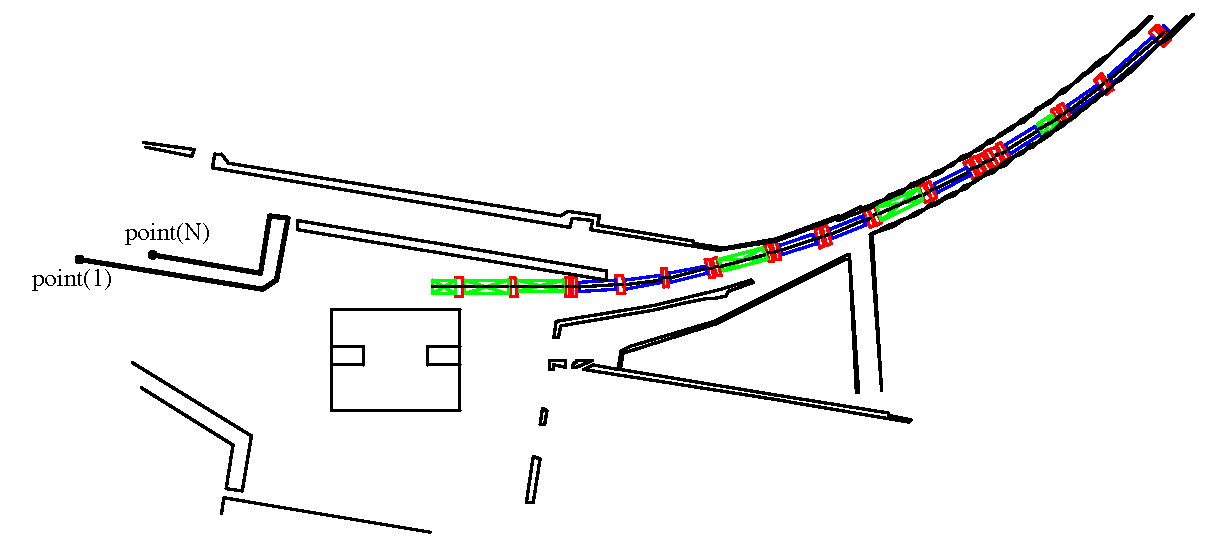
\includegraphics[width=5in]{building-wall.pdf}
  \caption[Floor_plan drawing showing the walls of the building]
{Floor_plan drawing showing the walls of the building (along with a section of a recirculation
arc). Defining building walls can be useful for such things as floor plots and designing a machine
to fit in an existing building.}
  \label{f:building.wall}
\end{figure}

A two dimensional cross-section of the building containing the machine under simulation may be defined in
\tao. This can be useful when drawing \vn{floor_plan} plots of the machine (\sref{s:floor.plan}) or
to design a machine to fit within an existing building by using optimization (\sref{c:opti}).

The wall cross-sections are defined by a set of ``\vn{sections}''. A section is a curve in the
horizontal $Z$-$X$ plane that defines where the face of a wall is. One such section is highlighted in
Figure~\ref{f:building.wall} starting at the point marked ``point(1)'' and ending at the point
marked ``point(N)''. Each section is defined by a set of points which are connected together using
straight lines or circular arcs.

The name of the file containing the building wall definition is given by the \vn{building_wall_file}
variable in the \vn{tao_start} namelist (\sref{s:init.global}). In general, this file will contain a
number of \vn{building_wall_section} namelists. Each \vn{building_wall_section} namelist defines a
single wall section. The syntax of this namelist is
\begin{example}
  &building_wall_section
    \{name = <string>\}
    \{constraint = <type>\}
    point(1) = <z1>, <x1>
    point(2) = <z2>, <x2>, \{<r2>\}
    point(3) = <z3>, <x3>, \{<r3>\}
    ... etc ...
    point(N) = <zN>, <xN>, \{<rN>\}
  /
\end{example}
The optional \vn{name} component allows for matching wall sections to \vn{floor_plan} shapes
(\sref{s:shapes}) when drawing a \vn{floor_plan} so that different portions of the wall can be drawn
in different colors.

The global coordinate system in \bmad (see the \bmad manual) defines the $(Z, X)$ plane as being
horizontal.  [Note: $(Z, X)$ is used instead of $(X, Z)$ since $(Z, X, Y)$ forms a right handed
coordinate system.] The points that define a wall section are specified in this coordinate system.
In the \vn{building_wall_section} namelist, the $(Z, X)$ position of each point defining a wall
section is given along with an optional radius $r$. If a non-zero radius is given for point $j$,
then the segment between point $j-1$ and $j$ is a circular arc of the given radius. If no radius is
given, or if it is zero, the segment is a straight line. A radius for the first point, number 1,
cannot be specified since this does not make sense. Additionally, a radius must be at least half the
distance between the two points that define the end points of the arc.

In general, given two end points and a radius, there are four possible arcs that can be drawn. The
arc chosen follows the following convention:
\begin{enumerate}
\item
The angle subtended by the arc is 180 degrees or less.
\item
If the radius for the arc from $j-1$ to $j$ is positive, the arc curves in a clockwise manner. If
the radius is negative, the arc curves counterclockwise. This convention mimics the convention used
for \vn{rbend} and \vn{sbend} elements.
\end{enumerate}
To define a wall that is circular, use three points with two 180
degree arcs in between.

When designing a machine to fit within the walls of a building, the \vn{constraint} variable of the
namelist is used to designate whether the given wall section is on the $+x$ (left) side of the
machine or the $-x$ (right) side. Here $x$ is the local reference frame transverse coordinate. See
the write up of the \vn{wall.right_side} and \vn{wall.left_side} constraints in \sref{s:data.types}
for more details. Possible values for \vn{constraint} are:
\begin{example}
  "right_side"  ! Section is to be used with wall.right_side constraints
  "left_side"   ! Section is to be used with wall.left_side constraints
  "none"        ! Default. Section is ignored in any constraint calculation.
\end{example}
Using \vn{"none"} for \vn{constraint} is convenient for drawing building components on a
\vn{floor_plan} that are not used as an optimization constraint.

Example:
\begin{example}
  &building_wall_section
    constraint = "left_side"   
    point(1) =  23.2837,    8.2842
    point(2) = -10.9703,   13.8712,   107.345
    point(3) = -10.8229,   14.7737
  /
\end{example}
In this example, point 1 is at $(Z, X) = (23.2837, 8.2842)$, the segment between points 1 and 2 is
an arc with a radius of 107.345 meters, and the segment between points 2 and 3 is a straight
line. Also this wall section is to be used when evaluating any \vn{wall.x+} constraint.

If the machine varies vertically ($y$-direction), vertical constraints may be imposed using the
\vn{floor.y} data type (\sref{s:data.types}).

To see a list of the building wall points when running \tao, use the \vn{show building_wall}
(\sref{s:show.building}) command .

Note: To position a machine in the global coordinate system, the starting point and starting
orientation can be adjusted using \vn{beginning[...]} statements as explained in the \bmad manual.

%-----------------------------------------------------------------
\subsection{Building Orientation}
\label{s:building.orient}

It may be convenient to use a different two-dimensional coordinate system for the horizontal plane
than the global coordinate system used by \bmad and \tao. For example, if the building wall coordinates are
obtained from a blueprint. To help with this, an overall position and angle
shift may be specified by a \vn{building_wall_orientation} namelist in the same file with the
\vn{building_wall_section} namelists. The syntax of the \vn{building_wall_orientation} namelist is:
\begin{example}
  theta = <Real>      ! Angle rotation in radians. Default is 0.
  z_offset = <Real>   ! Z-offset. Default is 0.
  x_offset = <Real>   ! X-offset. Default is 0.
\end{example}
The transformation from the input coordinates of a wall point specified in a \vn{build_wall_section} namelist
to the global coordinate system is
\begin{equation}
  \begin{pmatrix} z \\ x \end{pmatrix}_{global} = 
  \begin{pmatrix} \text{z_offset} \\ \text{x_offset} \end{pmatrix} +
  \begin{pmatrix} \cos(\text{theta}) & -\sin(\text{theta}) \\
                   \sin(\text{theta}) & \cos(\text{theta}) \end{pmatrix} \,
  \begin{pmatrix} z \\ x \end{pmatrix}_{input} 
\end{equation}

%-----------------------------------------------------------------
\section{Dynamic Aperture Calculation Initialization}
\index{dynamic aperture}
\label{s:dynamicaperture}

\begin{figure}
  \centering
  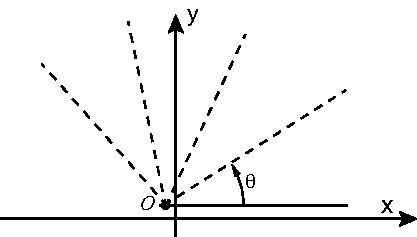
\includegraphics[width=5in]{dynamic-aperture-rays.pdf}
  \caption{
The calculation of a dynamic aperture curve in the $x$-$y$ plane at a given \vn{pz} offset involves
calculating aperture curve points (blue dots) along a set of ``rays'' (dashed lines) having a common
origin point ($\cal O$). The aperture curve is then constructed using linear interpolation between
points. The calculation of an aperture curve point along a given ray involves iteratively tracking
particles with different starting $(x, y)$ position values to find the boundary between stable
(green dots) and unstable (red dots) motion.
  }
  \label{f:da-rays}
\end{figure}

For rings, the dynamic aperture can be calculated and plotted. To calculate the dynamic aperture for
the $i$\Th universe, the \vn{design(i)%dynamic_aperture_calc} parameter must be set True in the
\vn{tao_design_lattice} namelist (\sref{s:init.lat}. Example:
\begin{example}
  &tao_design_lattice
    design_lattice(1)%file = "lat.bmad"
    design_lattice(1)%dynamic_aperture_calc = T
  /
\end{example}
Alternatively, the aperture calculation can be turned on during running using the \vn{set} command
(\sref{s:set.universe}):
\begin{example}
  set universe 1 dynamic_aperture_calc on
\end{example}
Since aperture calculations take time, once an aperture calculation is done, the calculation is
turned off so to perform multiple scans within a given session, the \vn{set universe} command must
be repeatedly done.

The \vn{show dynamic_aperture} command (\sref{s:show.da}) shows parameter values and the
\vn{set dynamic_aperture} command (\sref{s:set.da}) can be used to change parameter values.

If Tao is compiled with the appropriate OpenMP flags, the dynamic aperture calculation will be done
in parallel.

To plot the results, an appropriate plot must be defined (\sref{s:dynamic.ap.plot}) and
\vn{placed} in the plotting window (\sref{s:init.plot}. An example dynamic aperture plot is
shown in Fig.~\ref{f:da-plot}.

Example input files for calculating and plotting the dynamic aperture are at (\sref{s:examples}):
\begin{example}
  \$ACC_ROOT_DIR/tao/examples/dynamic_aperture
\end{example}

Parameters for the dynamic aperture simulation are set in the \vn{tao_dynamic_aperture}
namelist (\sref{s:init.global} in the \tao root initialization file. Example:
\begin{example}
  ! This defines parameters for universe 1.
  &tao_dynamic_aperture
   da_init(1)%ix_branch = 0         ! Lattice branch to use. 0 = default value.
   da_init(1)%pz = 0, 0.01, 0.15    ! List of particle phase space pz.
   da_init(1)%n_angle = 64          ! Number of angles in scan of each energy
   da_init(1)%min_angle = 0         ! Starting scan angle (rad).
   da_init(1)%max_angle = 3.14159   ! Ending scan angle (rad).
   da_init(1)%n_turn = 2000         ! Number of turns a particle must survive
   da_init(1)%x_init = 1e-3         ! initial estimate for horizontal aperture (meters).
   da_init(1)%y_init = 1e-3         ! initial estimate for vertical aperture (meters).
   da_init(1)%accuracy = 1e-5       ! resolution of bracketed aperture (meters)
  /
\end{example}
Dynamic aperture parameters can be defined for each universe. In the above example, parameters are
defined for universe 1. The \vn{pz} parameter array is a list of relative momenta to calculate the
aperture for. One dynamic aperture curve will be produced for each value of \vn{pz}. A dynamic
aperture curve represents the boundary in the $x$-$y$ plane such that if a particle is started with
$p_z$ equal to the given \vn{pz}, and with starting $p_x$, $p_y$, and $z$ set as
described below, then starting the particle with $(x, y)$ coordinates outside of the aperture curve
will result in particle loss and starting the particle with $(x, y)$ coordinates inside the curve
will result in particle survival. Here loss (``unstable motion'') and survival (``stable motion'')
is defined by whether the particle hits an aperture or not over the number of turns set by
\vn{%n_turn} (which is set to 2000 in the above example). The \vn{%ix_branch} parameter sets 
which branch in the lattice is used for tracking.

The calculation of an aperture curve is illustrated in Fig.~\ref{f:da-plot}. To calculate an
aperture curve, a set of ``rays" (dashed lines) having a common origin point ($\cal O$) are
constructed. On each ray, the boundary point between stable and unstable motion (blue points in the
figure) is found by iteratively tracking particles with initial $(x, y)$ points on the ray. The
aperture curve is then constructed using linear interpolation between points. The accuracy with
which the boundary points are calculated is set by the \vn{%accuracy} parameter. The \vn{%x_init}
and \vn{%y_init} values are used as a staring point for the boundary point search. The computed
boundary curve will not depend upon these parameters but having initial values close to the boundary
will same some computation time.

If the RF is off, the origin point of the rays is taken to be the closed orbit at the given
$p_z$. In this case, initial $p_x$ and $p_y$ are set to the closed orbit values, and $z$ is set to
zero (the motion is independent of $z$ so this set does not matter). If the RF is on, the origin
point, along with initial $p_x$, $p_y$, and $z$, are taken equal to the closed orbit (which is not
affected by the initial $p_z$).

The number of rays used is set by the \vn{%n_angle} parameter. In the above example, \vn{n_angle} is
set to 64. The angle of the rays with respect to the $x$-axis ($\theta$ in the figure) will range
from \vn{%min_angle} to \vn{%max_angle}. In the example above the angle ranges from 0 to $pi$.  That
is, the upper half-plane. These are typical settings since typically storage rings are vertically
symmetric so the aperture curves should vertically symmetric as well. The angle between rays is not
uniform but is adjusted to give roughly equally spaced points (this is done by looking at the aperture
points on a horizontal and a vertical ray and then scaling the ray angles appropriately).

%-----------------------------------------------------------------
\section{Initializing Plotting}
\index{plotting initializing}
\label{s:init.plot} 

\subsection{Plot Window}
\label{s:plot.page}
\index{initialization!plotting!plot window}

Plotting is defined by an initialization file whose name is defined by the \vn{plot_file} component
of the \vn{tao_start} namelist (\sref{s:init.global}).  The first namelist block in the file has a
block name of \vn{tao_plot_page}. This block sets the size of the plot window (also called the plot
page) and defines the ``regions'' where plots go. The syntax of this block is:
\index{tao_plot_page}\index{plot_page!n_curve_pts}
\index{plot_page!size}\index{plot_page!border}
\index{plot_page!text_height}\index{plot_page!title}
\index{region!name}\index{region!location}\index{place}
\begin{example}
  &tao_plot_page
    plot_page%plot_display_type        = <string>  ! Display type: "X" or "TK"
    plot_page%size                     = <x_size>, <y_size>         ! size in POINTS 
    plot_page%border                   = <x1\(_{\dstyle{b}}\)>, <x2\(_{\dstyle{b}}\)>, <y1\(_{\dstyle{b}}\)>, <y2\(_{\dstyle{b}}\)>, "<units>"
    plot_page%text_height              = <real>   ! height in POINTS. Def = 12
    plot_page%main_title_text_scale    = <real>   ! Relative to text_height. Def = 1.3
    plot_page%graph_title_text_scale   = <real>   ! Relative to text_height. Def = 1.1
    plot_page%axis_number_text_scale   = <real>   ! Relative to text_height. Def = 0.9
    plot_page%axis_label_text_scale    = <real>   ! Relative to text_height. Def = 1.0
    plot_page%legend_text_scale        = <real>   ! Relative to text_height. Def = 0.8
    plot_page%key_table_text_scale     = <real>   ! Relative to text_height. Def = 0.9
    plot_page%floor_plan_shape_scale   = <real>   ! Floor_plan shape size scaling.
    plot_page%lat_layout_shape_scale   = <real>   ! Lat_layout shape size scaling.
    plot_page%title(i)                 = <string>, {<x>, <y>, "<units>", "<justify>"}
    plot_page%n_curve_pts              = <int>    ! Num points used to construct a 
                                                  !   smooth curve. Default = 401
    plot_page%box_plots                = <T/F>    ! For debugging. Default = F.
    plot_page%delete_overlapping_plots = <T/F>    ! Default = T.
    plot_page%draw_graph_title_suffix  = <T/F>    ! Default = T.
    include_default_plots              = <T/F>    ! Include default templates? Def = T.
    region(i) = "<region_name>" <x1\(_{\dstyle{r}}\)>, <x2\(_{\dstyle{r}}\)>, <y1\(_{\dstyle{r}}\)>, <y2\(_{\dstyle{r}}\)>  
    place(i)  = "<region_name>", "<template_name>"
    default_plot%...                            ! See below.
    default_graph%...                           ! See below. 
  /
\end{example}

%-----------------------

\begin{figure}[bt]
  \centering
  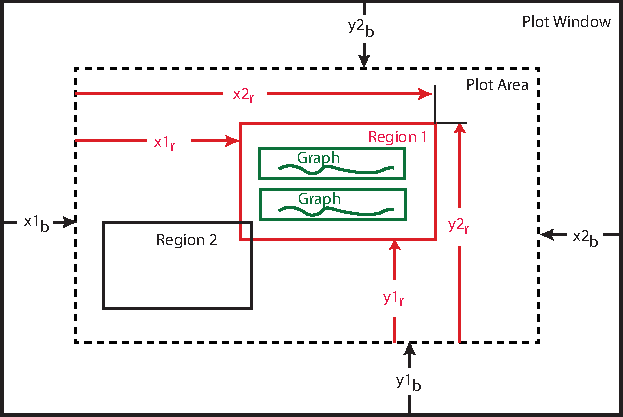
\includegraphics{plot-page.pdf}
  \caption[The plot window.]{The plot window has a boarder whose position is determined by 
the \vn{plot_page\%border} parameter in the tao_plot_page namelist.  Plots are placed
in ``\vn{regions}'' whose location is determined by the setting of the \vn{region(i)} parameters in
the same namelist. Regions may overlap.} 
  \label{f:plot.page}
\end{figure}

%-----------------------

For example:
\begin{example}
  &tao_plot_page
    plot_page%plot_display_type = "X"        ! X11 window.  "TK" is alternative.
    plot_page%size        = 700, 800         ! Points
    plot_page%border      = 0, 0, 0, 50, "POINTS"  
    plot_page%text_height = 12.0
    plot_page%title(1)    = "CESR Lattice", 0.5, 0.996, "%PAGE", "CC"
    region(1) = "top"    0.0, 1.0, 0.5, 1.0
    region(2) = "bottom" 0.0, 1.0, 0.0, 0.5
    place(1)  = "top",    "orbit"
    place(2)  = "bottom", "phase"
    default_plot%x%min = 100
    default_plot%x%max = 200
  /
\end{example}

\vn{plot_page%size} sets the horizontal and vertical size of the plot
window in \vn{points} units (72 points = 1 inch. Roughly 1 point = 1
pixel). 

\vn{plot_page%text_height} sets the overall height of the text that is
drawn. Relative to this, various parameters can be used to scale
individual types of text:
\begin{example}
  plot_page%main_title_text_scale  = 1.3 ! Main title height. 
  plot_page%graph_title_text_scale = 1.1 ! Graph title height.
  plot_page%axis_number_text_scale = 0.9 ! Axis number height
  plot_page%axis_label_text_scale  = 1.0 ! Axis label height.
  plot_page%key_table_text_scale   = 0.8 ! Key Table text (\sref{s:key.table}).
  plot_page%legend_text_scale      = 0.9 ! Lat Layout or floor plan text.
\end{example}
The default values for these scales are given above.

The \vn{plot_page%plot_display_type} component sets the type of plot display
window used. possibilities are:
\begin{example}
  "X"      X11 window
  "TK"     tk window
  "QT"     Available only when using PLPLOT (and not the default PGPLOT)
\end{example}
Note: The environmental variable \vn{ACC_PLOT_DISPLAY_TYPE} sets the default display
type. You can set this variable in your login file to avoid having to setup a \tao
init file to set this.

\vn{plot_page%border} sets a border around the edges of the window. As shown in
Figure~\ref{f:plot.page} x1$_{\dstyle{b}}$, x2$_{\dstyle{b}}$ are the right and left border widths
and y1$_{\dstyle{b}}$ and y2$_{\dstyle{b}}$ are the bottom and top border widths respectively.  The
rectangle within this border is called the plot area.

\vn{plot_page%title(i)} set the page title. There are two title areas (i = 1,2). If only the title
string is given then the other variables are set to the defaults \vn{x} = 0.5, \vn{y} = 0.995,
\vn{justify} = "CC" and \vn{units} = "\vn{%PAGE}". See the QuickPlot documentation
(\sref{s:line.symb}) for more details.

The plot area is divided up into rectangular regions where plots may be placed (what defines a plot
is discussed below).  \vn{region(i)} in the \vn{tao_plot_page} namelist is an array of five elements
that defines the i\Th region. The first element of this array is the name of the region. This name
may not contain a dot ``.''.  The last four elements of the \vn{retion(i)} array, x1$_{\dstyle{r}}$,
x2$_{\dstyle{r}}$, y1$_{\dstyle{r}}$ and y2$_{\dstyle{r}}$ define the location of the region as
illustrated in Figure~\ref{f:plot.page}.  x1$_{\dstyle{r}}$ and x2$_{\dstyle{r}}$ are normalized to
the width of the plot area and y1$_{\dstyle{r}}$ and y2$_{\dstyle{r}}$ are normalized to the height
of the plot area. That is, these four number should be in the range $[0, 1]$.  Regions may overlap
any one can define as many regions as one likes.

Besides the regions that the user sets up in the \vn{tao_plot_page} namelist, \tao defines a number
of default regions whose names begin with the letter ``\vn{r}''. Use the \vn{show plot} command
(\sref{s:plot}) to view a list of these plots.

When \vn{plot_page%delete_overlapping_plots} is True (the default), Placing a plot (using
the \vn{place} command \sref{s:place}) causes any existing plots that overlap the
placed plot to become invisible. 

The \vn{plot_page%draw_graph_title_suffix} is used to suppress the drawing of the string that
is printed to the right of a graph title (set by \vn{graph%title}). This string is set by \tao
and has information on what is being plotted (typically the \vn{curve%component}). To suppress
the suffix, set \vn{plot_page%draw_graph_title_suffix} to False.

The \vn{plot_page%n_curve_pts} parameter sets the default number of points to use for drawing
``smooth'' curves. The default is 401. This default may be overridden for individual plots by
setting the \vn{plot%n_curve_pts} component of a plot (\sref{s:template}). If \vn{plot%n_curve_pts}
is set for an individual plot, that value overrides the value of
\vn{plot_page%n_curve_pts}. Warning: \tao will cache intermediate calculations used to compute a
smooth curve to use in the computation of other smooth curves. \tao will only do this for curves
that have \vn{plot_page%n_curve_pts} number of points. Depending upon the circumstances, setting
\vn{plot%n_curve_pts} for individual plots may slow down plotting calculations significantly.

The \vn{place(i)} commands, $i = 1,2,3,\ldots$ determine the initial placement of plots. The initial
placement can be modified while \tao is running using the \vn{place} command (\sref{s:place}).

\vn{default_plot} sets the defaults for any \vn{plot}s defined in the \vn{tao_template_plot}
namelists (\sref{s:template}). Similarly, \vn{default_graph} sets defaults for the \vn{graph}
structure defined in the \vn{tao_template_graph} namelist (\sref{s:template}). In the example above,
the default x-axis min and max are set to 100 and 200 respectively.

If \vn{include_default_plots} is set to \vn{False}, the collection of default template
plots (\sref{s:template}) that \tao uses by default are not used along with the template
plots defined in the plotting file.

%-----------------------------------------------------------------
\subsection{Plot Templates}
\label{s:template}
\index{plot templates}

As shown in Figure~\ref{f:plot}, a ``plot'' is made up of a collection of ``graphs'' and a graph
consists of axes plus a set of ``curves''. To define custom plots, there needs to be defined
a set of ``template plots''. A template plot specifies the layout of a plot: How the graphs are
placed within a plot, what curves are associated with what graphs, etc. When running \tao, the
information in a template plot may then be transferred to a region using the \vn{place} command and
this will produce a visible plot.

The file that \tao looks in to find plotting information is set by the \vn{plot_file} component of
the \vn{tao_start} namelist (\sref{s:init.global}). The default, if \vn{plot_file} is not set, is
the root initialization file.

Template plots are defined using namelists with a name of \vn{tao_template_graph}. The general
syntax is:
\index{tao_template_plot}
\index{plot!name}
\index{plot!x}
\index{plot!x_axis_type}
\index{plot!n_graph}
\index{plot!autoscale_gang_x}
\index{plot!autoscale_gang_y}
\index{plot!autoscale_x}
\index{plot!autoscale_y}
\begin{example}
  &tao_template_plot
    plot%name        = "<plot_name>"
    plot%x           = <qp_axis_struct>
    plot%x_axis_type = "<x_axis_type>"   ! "index", "ele_index" "s", "lat", "var", etc. 
    plot%n_graph     = <n_graphs>
    plot%autoscale_gang_x = <logical>    ! Default: True.
    plot%autoscale_gang_y = <logical>    ! Default: True.
    plot%autoscale_x = <logical>         ! Default: False.
    plot%autoscale_y = <logical>         ! Default: False.
    plot%n_curve_pts = <integer>         ! Used to override plot_page%n_curve_pts.
    default_graph%...                    ! See below
  /
\end{example}
For example:
\begin{example}
  &tao_template_plot
    plot%name                = "orbit"
    plot%x%min               =   0
    plot%x%max               = 100
    plot%x%major_div_nominal = 10
    plot%x%label             = "Index"
    plot%n_graph             = 2
    default_graph%y%max      = 10
  /
\end{example}

\vn{default_graph} sets defaults for the \vn{graph} structure defined in the \vn{tao_template_graph}
namelist (\sref{s:template}). This overrides \vn{default_graph} settings made in the
\vn{tao_template_plot} namelist (\sref{s:init.plot}) but only for graphs associated with the
\vn{tao_template_plot} the \vn{default_graph} is defined in.

\vn{plot%x} sets the properties of the horizontal axis. For more information see the \vn{QuickPlot}
documentation (\sref{s:line.symb}) on the \vn{qp_axis_struct}.  If \vn{min} and \vn{max} are absent,
then \tao will autoscale the axis.  If it is desired to have differing scales for different graphs,
the \vn{graph%x} component can be used (see below).

Both \vn{major_div} and \vn{major_div_nominal} set the number of major divisions in the plot. The
difference between the two is that with \vn{major_div} the number of major divisions is fixed at the
set value and with \vn{major_div_nominal} the number of major divisions can vary from the set value
when \tao scales a graph. If \vn{major_div_nominal} is set, this will override any setting of
\vn{major_div}. If neither \vn{major_div} nor \vn{major_div_nominal} is set, a value will be chosen
for \vn{major_div_nominal} by \tao. If you are unsure which to set, it is recommended that
\vn{major_div_nominal} be used.

Plots with \vn{plot%autoscale_x} and/or \vn{plot%autoscale_y} logicals, set to true will
automatically rescale after any calculation. The \vn{plot%autoscale_gang_x} and
\vn{plot%autoscale_gang_y} components set how the \vn{x_scale} (\sref{s:x.scale}) and \vn{scale}
(\sref{s:scale}) commands behave when autoscaling entire plots. See these individual commands for
more details.

The \vn{plot%n_plot_pts} parameter sets the number of points to use for drawing ``smooth''
curves. This overrides the setting of \vn{plot_page%n_plot_pts} (\sref{s:init.plot}). Warning: \tao
will cache intermediate calculations used to compute a smooth curve to use in the computation of
other smooth curves. \tao will only do this for curves that have \vn{plot_page%n_curve_pts} number
of points. Depending upon the circumstances, setting \vn{plot%n_curve_pts} for individual plots may
slow down plotting calculations significantly.

\vn{plot%name} is the name that is used with \tao commands to identify the plot. It is important
that this name not contain any blank spaces since \tao uses this fact in parsing the command line.

\vn{plot%x_axis_type} sets what is plotted along the
\vn{x_axis}. Possibilities are:
\index{index}
\index{ele_index}
\index{s}
\begin{example}
    "index"         ! Data Index.
    "ele_index"     ! Element lattice number index.
    "s"             ! Longitudinal position in the lattice.
    "s_expression"  ! s-dependent expression involving lattice parameters.
    "data"          ! From a data array.
    "lat"           ! Lattice variable. See \sref{s:plot.var}.
    "var"           ! Tao variable value. See \sref{s:plot.var}.
    "phase_space"   ! Set by \tao if graph%type = "phase_space".
    "none"          ! Set by \tao if graph%type = "key_table".
    "floor"         ! Set by \tao if graph%type = "floor_plan".
\end{example}

The \vn{ele_index} switch is used when plotting data arrays. In this
case the \vn{index} switch refers to the index of the data array and
\vn{ele_index} refers to the index of the lattice element that the
datum was evaluated at.

\vn{n_graph} sets the number of graphs associated with the plot and
each one needs a \vn{tao_template_graph} namelist to define it. These
namelists should be placed directly after their respective
\vn{tao_template_graph} namelists. The general format of the
\vn{tao_template_graph} namelist is:
\index{tao_template_graph}\index{graph!y}\index{curve!name}
\index{graph_index}\index{graph}\index{graph!name}\index{curve}
\index{graph!type}\index{graph!box}\index{graph!title}\index{graph!margin}
\index{graph!y2}\index{graph!n_curve}\index{graph!clip}\index{graph!component}
\index{graph!symbol_size_scale}
\index{curve!data_type}\index{curve!data_source}
\index{curve!x_axis_units_factor}\index{curve!y_axis_units_factor}
\index{curve!use_y2}\index{curve!line}\index{curve!ele_ref_name}
\index{curve!draw_line}\index{curve!draw_symbols}\index{curve!ix_universe}
\index{curve!symbol}\index{curve!symbol_every}\index{curve!convert}
\index{curve!ix_bunch}\index{curve!data_type_x}
\begin{example}
  &tao_template_graph
    graph_index             = <integer>
    graph%name              = "<string>"       ! Default is  "g<n>" <n> = graph_index. 
    graph%type              = "<string>"       ! "data", "floor_plan", etc.
    graph%box               = <ix>, <iy>, <ix_tot>, <iy_tot>
    graph%title             = "<string>"       ! Title above the graph.
    graph%title_suffix                         ! Not user settable.
    graph%margin            =  <ix1>, <ix2>, <iy1>, <iy2>, "<Units>"
    graph%scale_margin      =  <ix1>, <ix2>, <iy1>, <iy2>, "<Units>"
    graph%x                 = <qp_axis_struct> ! Horizontal axis.
    graph%y                 = <qp_axis_struct> ! Left axis.
    graph%x2                = <qp_axis_struct> ! Top axis (only used for floor_plan plots).
    graph%y2                = <qp_axis_struct> ! Right axis.
    graph%y2_mirrors_y      = <logical>        ! y2 min/max the same as y-axis? Default = T
    graph%clip              = <logical>        ! Clip curves at boundary? Default = T
    graph%draw_axes         = <logical>        ! Default = T
    graph%draw_grid         = <logical>        ! Default = T
    graph%allow_wrap_around = <logical>        ! Wrap curves around lattice ends?
    graph%component         = "<string>"       ! Eg: "model - design"
    graph%symbol_size_scale = <real>                  ! Phase_space plots symbol scale factor
    graph%ix_universe       = <integer>               ! Default = -1 => Use default universe
    graph%floor_plan        =  <floor_plan_struct>    ! Floor_plan parameters (\sref{s:floor.plan}).
    graph%draw_only_good_user_data_or_vars     ! Veto data or variables with good_user = F?
                                 = <logical>   !   Default = T.
    graph%x_axis_scale_factor    = <factor>    ! Scale the x-axis by this.
    graph%n_curve                = <integer>   ! number of curves
    curve(i)%name                = "<string>"  ! Default is "c<i>", <i> = curve num.
    curve(i)%data_source         = "<string>"  ! Source for the data curve points
    curve(i)%data_type_x         = "<string>"  ! Used with plot%x_axis_type = "data" or "var".
    curve(i)%data_type           = "<string>"  ! EG: "orbit.x"
    curve(i)%component           = "<string>"  ! Eg: "model - design". Overrides graph%component.
    curve(i)%data_index          = "<string>"  ! Index number for data points.
    curve(i)%legend_text         = "<string>"  ! Text for curve legend. 
                                               !   Default is the data_type.
    curve(i)%y_axis_scale_factor = <factor>    ! Scale the y-axis by this.
    curve(i)%use_y2              = <logical>   ! Use left-axis scale?
    curve(i)%draw_line           = <logical>   ! Connect data with lines?
    curve(i)%draw_symbols        = <logical>   ! Draw data symbols?
    curve(i)%draw_symbol_index   = <logical>   ! Print index number next to the data symbol?
    curve(i)%draw_error_bars     = <logical>   ! Draw error bars with data?
    curve(i)%ix_universe         = <integer>   ! Default = -1 => Use graph%ix_universe.
    curve(i)%ix_branch           = <integer>   ! Default = 0  => Use main lattice.  
    curve(i)%ix_bunch            = <integer>   ! Bunch index. Default = 0 (all bunches).
    curve(i)%line        = <qp_line_struct>    ! Line spec (color, width, etc.)
    curve(i)%symbol      = <qp_symbol_struct>  ! Symbol spec (color size, etc.)
    curve(i)%symbol_every     = <integer>      ! Plot symbol every # datums
    curve(i)%ele_ref_name     = "<string>"     ! Name of reference element.
    curve(i)%smooth_line_calc = <Logical>      ! Calc data between symbol points? 
    curve(i)%units            = "<string>"     ! Data units
  /
\end{example}
For example:
\begin{example}
  &tao_template_graph
    graph_index               = 1
    graph%name                = "x"
    graph%type                = "data"
    graph%box                 = 1, 1, 1, 2
    graph%title               = "Horizontal Orbit (mm)"
    graph%margin              =  60, 200, 30, 30, "POINTS"
    graph%y%label             = "X"
    graph%y%max               =  4
    graph%y%min               = -4
    graph%y%major_div_nominal = 4
    graph%n_curve             = 1
    graph%component           = "model - design"
    curve(1)%data_source      = "data"
    curve(1)%data_type        = "orbit.x"
    curve(1)%units_factor     = 1000
    curve(1)%use_y2           = F
  /
\end{example}
See the QuickPlot documentation (\sref{s:line.symb}) description of the \vn{qp_symbol_struct} and the
\vn{qp_line_struct}.

\vn{graph%title} is the string just above the graph. The full string will also include information
about what is being plotted and the horizontal axis type. To fully suppress the title leave it
blank. Note: A graph also has a \vn{graph%title_suffix} which \tao uses to hold the string which is
printed to the right of the \vn{graph%title}. This string contains information like what
\vn{curve%component} is being plotted. The \vn{graph%title_suffix} cannot be set by the user.

If there are multiple curves drawn with a graph then a curve legend showing what lines are
associated with what data will be drawn. The default is to draw this legend in the upper left hand
corner of the graph. By default, the \vn{data_type} of each curve will be used as the text for that
curve's line in the legend.  This default can be changed by setting a curve's \vn{curve%legend_tex}.

\vn{graph%name} and \vn{curve%name} define names to be used with commands. The default names are
just the letter \vn{g} or \vn{c} with the index of the graph or curve. Thus, in the example above,
the name of the curve defaults to \vn{c1} and it would be referred to as \vn{orbit.x.c1}.  It is
important that these names do not contain any blank spaces since \tao uses this fact in parsing the
command line.

\vn{graph%box} sets the layout of the box which the \vn{graph} is placed in. For a definition of
what a box is see the QuickPlot documentation (\sref{s:line.symb}). In the above example the graph
divides the region into two vertically stacked boxes and places itself into the bottom one.

\vn{graph%allow_wrap_around} sets if, for a lattice with closed geometry, the curves contained in
the graph are ``wrapped'' around the end of the lattice if \vn{graph%x%min} is negative. The default
is \vn{True}. This only applies if \vn{plot%x_axis_type} is set to \vn{"s"}.

\vn{graph%margin} sets the margin between the \vn{graph} and the \vn{box}
it is drawn in.

\vn{graph%scale_margin} is used to set the minimum space between what is being drawn and the edges
of the \vn{graph} when a \vn{scale}, \vn{x_scale}, or a \vn{xy_scale} command is issued. Normally
this is zero but is useful for \vn{floor plan} drawings.

\vn{graph%type} is the type of graph. \tao knows about the
following types:
\index{data}\index{lat_layout}\index{key_table}\index{phase_space}
\index{floor_plan}\index{beam_chamber_wall}
\begin{example}
  "data"               ! Lattice parameters, data and/or variable plots (default) (\sref{s:plot.data}).
  "dynamic_aperture"   ! Dynamic aperture plot (\sref{s:dynamic.ap.plot}
  "floor_plan"         ! A 2-dimensional birds-eye view of the machine (\sref{s:floor.plan}).
  "histogram"          ! Histogram of plot (\sref{s:histogram}).
  "key_table"          ! Key binding table for single mode (\sref{s:key.table}).
  "lat_layout"         ! Schematic showing placement of the lattice elements (\sref{s:lat.layout}).
  "phase_space"        ! Phase space plots (\sref{s:phase.space}).
\end{example}

With \vn{graph%type} set to \vn{"beam_chamber_wall"} (\sref{s:beam.wall.draw}), the beam chamber
wall is drawn if it has been defined in the \bmad lattice file.

With \vn{graph%type} set to \vn{"data"} (\sref{s:plot.data}), data such as orbits and/or variable
values such as quadrupole strengths are plotted. Here ``data'' can be data from a defined data
structure (\sref{c:data}) or computed directly from the lattice, beam tracking, etc. A \vn{"data"}
graph type will contain a number of \vn{curves} and multiple data and variable curves can be drawn
in one graph.

With \vn{graph%type} set to \vn{floor_plan} (\sref{s:floor.plan}), the two dimensional layout of the
machine is drawn.

With \vn{graph%type} set to \vn{histogram} (\sref{s:histogram}), such things such as beam densities
can be histogrammed.

With \vn{graph%type} set to \vn{"key_table"} (\sref{s:key.table}), the key bindings for use in
single mode (\sref{s:key.bind}) are displayed.  Note: The \vn{"key_table"} graph type does not have
any associated \vn{curve}s.

With \vn{graph%type} set to \vn{lat_layout} (\sref{s:lat.layout}), the elements of the lattice are
symbolical drawn in a one dimensional line as a function of the longitudinal distance along the
machine centerline.

With \vn{graph%type} set to \vn{phase_space} (\sref{s:phase.space}), phase space plots are produced.

%-----------------------------------------------------------------
\subsection{Lattice Parameters, Data and Variable plotting}
\label{s:plot.data}

A \vn{graph} (\sref{s:template}), with \vn{graph%type} equal to \vn{"data"}, is used to draw lattice
parameters such as orbits, or \tao data (\sref{c:data}), or variable values such as quadrupole
strengths. A data \vn{graph} will have a number of associated \vn{curve}s with each curve defining a
particular data type to plot.

The data values will depend upon where the data comes from. This is determined, in part, by the
setting of \vn{graph%component} and \vn{curve%component}. \vn{graph%component} and
\vn{curve%component} may be one of:
\index{model}\index{design}\index{base}\index{meas}\index{ref}
\begin{example}
  "model"             ! model values. Default.
  "design"            ! design values.
  "base"              ! Base values
  "meas"              ! data values.
  "ref"               ! reference data values.
  "beam_chamber_wall" ! Beam chamber wall
\end{example}
Additionally, \vn{graph%component} may be set to plot a linear combination of the above. For
example:
\begin{example}
  graph%component = "model - design"
\end{example}
This will plot the difference between the \vn{model} and \vn{design} values.

If \vn{curve%component} is set, it will override \vn{graph%component}. If \vn{graph%component} is
not set in the initialization file, and if there are curves of the graph that have not been set,
\vn{graph%component} will be given a default setting of \vn{model}.

\index{data}\index{var}\index{calculation}
\index{curve!data_source}
The \vn{curve} structure is used to define the data that is plotted in each graph.
\vn{curve%data_source} is the type of information for the source of the data points.
\vn{curve%data_source} must be one of:
\begin{example}
  "data"              ! A d1_data array is the source of the curve points.
  "var"               ! A v1_var array is the source of the curve points.
  "lat" (Default)     ! The curve points are computed directly from the lattice.
  "beam"              ! The curve points are computed tracking a beam of particles.
  "multi_turn_orbit"  ! Computation is from multi-turn tracking. 
\end{example}
The default for \vn{curve%data_source} is \vn{"lat"}. With \vn{curve%data_source} set to \vn{data},
the values of the curve points come from the \vn{d1_data} array structure named by
\vn{curve%data_type}. Thus in the above example the curve point values are obtained from
\vn{orbit.x} data. To be valid the data structure named by \vn{curve%data_type} must be set up in an
initialization file. If not given, the default \vn{curve%data_type} is
\begin{example}
  <plot%name>.<graph%name>
\end{example}
If \vn{curve%data_source} is set to \vn{var}, the values of the curve points come from a \vn{v1_var}
array structure. If it is set to \vn{lat} the curve data points are calculated from the lattice
without regard to any data structures. \vn{curve%data_source} can be set to \vn{beam} when tracking
beams of particles. In this case, the curve points are calculated from the tracking. With \vn{beam},
the particular bunch that the data is extracted from can be specified via \vn{curve%ix_bunch}. The
default is \vn{0} which combines all the bunches of the beam for the calculation.

Example: With \vn{curve%data_type} set to \vn{beta.x}, the setting of \vn{curve%data_source} to
\vn{lat} gives the beta as calculated from the lattice and \vn{beam} gives the beta as calculated
from the shape of the beam.

\vn{curve%draw_symbols} determines whether a symbol is drawn at the data points. The size, shape and
color of the symbols is determined by \vn{curve%symbol}. A given symbol point that is drawn has
three numbers attached to it: The $(x, y)$ position on the graph and an index number to help
identify it. The index number of a particular symbol is the index of the datum or variable
corresponding the symbol in the \vn{d1_data} or \vn{v1_var} array. These three numbers can be
printed using the \vn{show curve -symbol} command (\sref{s:show}).  \vn{curve%draw_symbol_index}
determines whether the index number is printed besides the symbol. Use the \vn{set curve} command
(\sref{s:set}) to toggle the drawing of symbols. The default value for \vn{curve%draw_symbol} is
False if \vn{plot%x_axis_type} is \vn{"s"}, \vn{"curve"}, \vn{"lat"}, or \vn{"var"} and True
otherwise. The default \vn{curve%draw_symbol_index} is always False.

\vn{curve%draw_line} determines whether a curve is drawn through the data point symbols. The
thickness, style (solid, dashed, etc.), and color of the line can be controlled by setting
\vn{curve%line}. If \vn{plot%x_axis_type} is \vn{"s"}, and \vn{graph%component} does not contain
\vn{"meas"} or \vn{"ref"}, \tao will attempt to calculate intermediate values in order to draw a
smooth, accurate curve is drawn. Occasionally, this process is too slow or not desired for other
reasons so setting \vn{curve%smooth_line_calc} to False will prevent this calculation and the curve
will be drawn as a series of lines connecting the symbols. The default of
\vn{curve%smooth_line_calc} is True. Use the \vn{set curve} command (\sref{s:set}) to toggle the
drawing of lines. Alternatively, the \vn{-disable_smooth_line_calc} switch can be used on the
command line (\sref{s:command.line}) or the global variable \vn{global%disable_smooth_line_calc} can
be set in the \tao initialization file (\sref{s:globals}).

The \vn{graph%draw_only_good_user_data_or_vars} logical determines whether datums
(\sref{s:init.data}) or variables (\sref{s:init.var}) with a \vn{good_user} component set to
\vn{False} are drawn. The default is to not draw them which means that data or variables not used in
an optimization are not drawn.

A graph has two vertical axes. The one on the left is called \vn{"y"} and the one on the right is
called \vn{"y2"}. For example, \vn{graph%y%label} sets the axis label for the \vn{y} axis and
\vn{graph%y2%label} sets the axis label for the \vn{y2} axis. Normally there is only one vertical
scale for a graph and this is associated with the \vn{y} axis. However, if any curve of a given
graph has \vn{curve%use_y2} set to \vn{True} then the \vn{y2} axis will have an independent second
scale. In this case, the \vn{y2} axis numbers will be drawn. Notice that simply giving the \vn{y2}
axis a label does {\em not} make the \vn{y2} axis scale independent of the \vn{y} axis scale.

Typically, a graph's horizontal scale is set by the \vn{plot%x} component. If it is desired to have
differing scales for different graphs, the \vn{graph%x} component can be used.

The \vn{curve%draw_error_bars} logical determines whether error bars are drawn when plotting data
(\vn{curve%data_source} set to \vn{data}). The half height of the error bars is determined by the
\vn{error_rms} values of the data associated with the curve (\sref{s:data.anatomy}).  To keep things
simple, \tao ignores the setting of \vn{curve%component} when drawing error bars. This must be kept
in mind since for example, the measurement error associated with a difference plot of measured data
- reference data (when \vn{curve%component} is set to \vn{meas-ref}) is different from just plotting
measured data, which in turn is different from a plot of the data as calculated from the \vn{model}
(the measurement error associated with this is zero).

The \vn{curve%ele_ref_name} component is only used if \vn{curve%data_source} is set to \vn{"lat"}.
If \vn{curve%ele_ref_name} is set, the curve will be shifted by subtracting the value of the
parameter being plotted evaluated at the reference element. For example, if \vn{orbit.x} is being
plotted, and \vn{curve%ele_ref_name} is set to "\vn{Q10W}", the plotted curve will be shifted by
subtracting the value of the horizontal orbit at Q10W. Notice that the shifting is done for each
graph component. For example, if \vn{graph%component} is set to "\vn{model - design}", the curve
will be shifted by subtracting the difference between the \vn{model} and \vn{design} values
evaluated at the reference element.

%-----------------------------------------------------------------
\subsection{Graphing a Data Slice}\index{plot!data slice}
\label{s:graph.data.slice}

Note: Data slicing is a type of parametric plotting. For parametric plotting using curve data see
section~\sref{s:param.plot}.

The standard data graph, as presented in the previous subsection, plots data from a given
\vn{d1_data} array. It is also possible to graph data that has been ``sliced'' in other ways. For
example, suppose a number of universes have been established, with each universe representing the
same machine but with different steerings powered. If in each universe an \vn{orbit} \vn{d2_data}
structure has been defined, an example of a data slice is the collection of points (x, y) where:
\begin{example}
  (x, y) = (<n>@orbit.x[23], <n>@orbit.y[23]),   <n> = 1, ..., n_universe
\end{example}
When defining a template for graphing a data slice, the plot%x_axis_type is set to \vn{"data"}, and
the \vn{graph%type} must be set to \vn{"data"}, the \vn{curve(:)%data_source} must be set to
\vn{"data"} and the \vn{curve(:)%data_type_x} and \vn{curve%data_type} are used to define the x and
y axes respectively.  In the strings given by \vn{<curve%data_type_x} or \vn{<curve%data_type}, all
substrings that look like \vn{\#ref} are eliminated and the string given by \vn{curve%ele_ref_name}
is substituted in its place.  Similarly, a \vn{\#comp} string is used as a place holder for the
\vn{graph%component} Example:
\begin{example}
  &tao_template_plot
    plot%name = "at_bpm"
    plot%x%label = "x"
    plot%x_axis_type = "data"
    plot%n_graph = 1
  /

  &tao_template_graph
    graph_index = 1
    graph%title = "Orbit at BPM"
    graph%y%label = "y"
    graph%component = "meas - ref"
    graph%type = "data"
    graph%n_curve = 1
    graph%x_axis_scale_factor = 1000
    curve(1)%data_source = "data"
    curve(1)%data_type_x = "[2:57]@orbit.x[#ref]|#comp"
    curve(1)%data_type   = "[2:57]@orbit.y[#ref]|#comp"
    curve(1)%data_index  = "[2:57]@orbit.y[#ref]|ix_uni"
    curve(1)%y_axis_scale_factor = 1000
    curve(1)%ele_ref_name = "23"
    curve(1)%draw_line = F
  /
\end{example}
In this example, \vn{curve(1)%data_type_x} expands to \vn{"[2:57]@orbit.x[23]|meas-ref"}. That is,
the \vn{meas - ref} values of \vn{orbit.x[23]} from universes 2 through 57 is used for the x-axis.
Similarly, \vn{orbit.y[23]} is used for the y-axis. The \vn{set} command (\sref{s:set}) can be used
to change \vn{curve%ele_ref_name} and \vn{graph%component} strings.

\vn{curve%data_index} sets the index number for the symbol points (\sref{s:template}). In the above
example, \vn{curve%data_index} is set to \vn{"[2:57]@orbit.y[\#ref]|ix_uni"}. The \vn{|ix_uni}
component will result in the symbol index number being the universe number.  Additionally, the
component \vn{|ix_d1} can be used to specify the index in the \vn{d1_data} array, and the component
\vn{|ix_ele} can be used to specify the lattice element index. Setting the symbol index number is
important when \vn{curve%draw_symbol_index} is set to True so that the symbol index is drawn with
the curve. Additionally, the command \vn{show curve -symbol} (\sref{s:show}) will print the symbol
index number along with the $(x, y)$ coordinates of the symbols.

Arithmetic expressions (\sref{s:arithmetic.exp}) may be mixed with explicit datum components in the
specification of \vn{curve(:)%data_type_x} and \vn{curve(:)%data_type}. Example:
\begin{example}
  curve(1)%data_type_x = "[#ref]@orbit.x|model"
  curve(1)%data_type   = "[#ref]@orbit.x|meas-ref"
  curve(1)%ele_ref_name = "3"
\end{example}
The plots the \vn{model} values of \vn{orbit.x} verses \vn{meas - ref} of \vn{orbit.x} for the data
in universe 3. Note: Whenever explicit components are specified, the \vn{graph%component} settings
are ignored for that expression.

%-----------------------------------------------------------------
\subsection{Plotting With a Variable Parameter on the X-Axis}
\index{plot!plotting as a function of a variable}
\label{s:plot.var}

Data can be plotted as a function of a lattice parameter by setting \vn{plot%x_axis_type} to
\vn{"lat"} (for lattice variables) or \vn{"var"} (for \tao variables) and setting
\vn{curve(:)%data_type_x} to the name of the variable. In this case, the \vn{curve(:)%data_type}
must evaluate to a single number.

Example:
\begin{example}
  &tao_template_plot
    plot%x_axis_type = "lat"
    plot%n_curve_pts = 50
    ...
  /

  &tao_template_graph
    ...
    curve(1)%data_type_x = "particle_start[x]"  ! X-axis values.
    curve(1)%data_type   = "orbit.x[10]"        ! Y-axis values.
    ...
  /
\end{example}
Here the number of curve points has been set to 50 to reduce the evaluation overhead.

Note: \tao treats the \vn{design} and \vn{base} lattices as static so that varying a variable will
not affect these lattices. Thus, constructing a plot with \vn{graph%component} set to, for example,
\vn{"model - design"} will {\em not} produce a plot that is the difference between varying a
variable in both \vn{model} and \vn{design} lattices. In the case where such a plot is desired, a
second universe needs to be established. In this case, one would set \vn{curve(:)%data_type} to
something like
\begin{example}
    curve(1)%data_type   = "1@orbit.x[10] - 2@orbit.x[10]"    
\end{example}
where the universe \#2 \vn{model} lattice would be setup to be equal to the universe \#1 \vn{design}
lattice.

%-----------------------------------------------------------------
\subsection{Drawing a Lattice Layout}
\index{lattice layout}
\label{s:lat.layout}

\begin{figure}
  \centering
  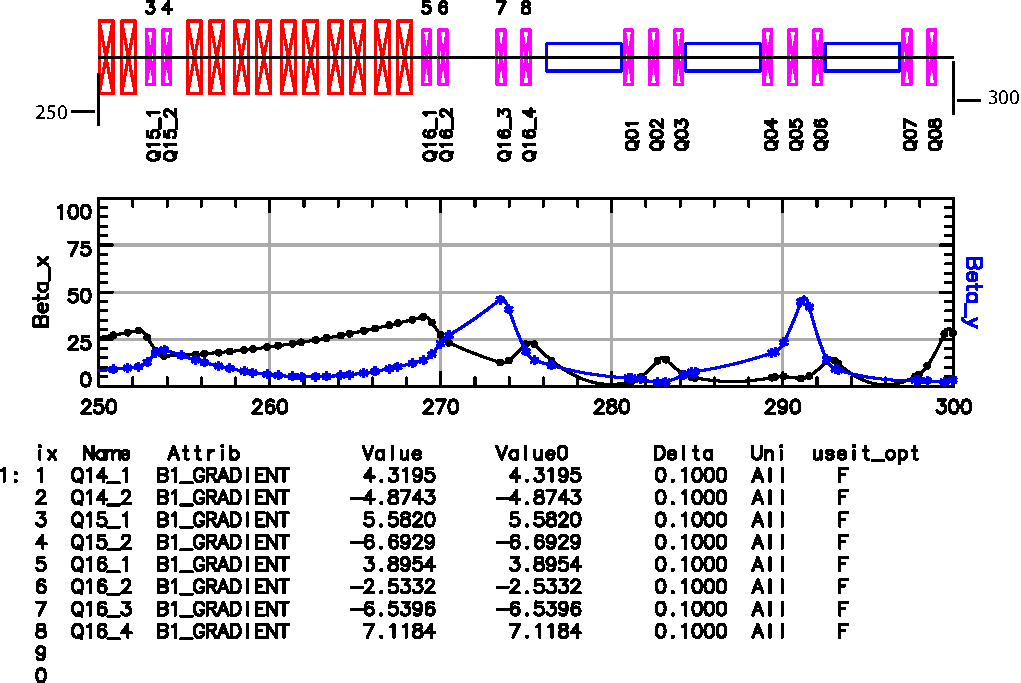
\includegraphics[width=5in]{layout-graph-table.pdf}
  \caption[Example lattice layout and data plots]
{A lattice layout plot (top) above a data plot (middle) which in turn is above a key table plot
(bottom). The points on the curves in the data plot mark the edges of the elements displayed in the
lattice layout. Elements that have attributes that are varied as shown in the key table have the
corresponding key table number printed above the element's glyph in the lattice layout.}
  \label{f:layout.table}
\end{figure}

A lattice layout plot draws the lattice along a straight line with colored rectangles representing
the various elements.  An example is shown in Figure~\ref{f:layout.table}.  The
\vn{tao_template_plot} needed to define a lattice layout looks like:
\index{tao_template_plot}\index{plot!name}
\index{plot!x!min}\index{plot!x!max}\index{plot!n_graph}
\index{tao_template_graph}\index{graph_index}\index{graph!name}
\index{graph!type}\index{graph!title}\index{graph!box}
\index{graph!ix_universe}\index{graph!margin}\index{graph!n_curve}
\begin{example}
  &tao_template_plot
    plot%name        = "<plot_name>"
    plot%x%min       = <real>  
    plot%x%max       = <real>  
    plot%n_graph     = <integer>
    plot%x_axis_type = "s"
  /
  &tao_template_graph
    graph_index       = <integer>
    graph%name        = <name>
    graph%type        = "lat_layout"
    graph%title       = "Layout Title"
    plot%box          = <ix>, <iy>, <ix_tot>, <iy_tot>
    graph%ix_universe = <integer> ! -1 => use current default universe
    graph%ix_branch   = <integer> !  0 => use main lattice.
    graph%margin      = <ix1>, <ix2>, <iy1>, <iy2>, "<Units>"
    graph%y%min       = <real>    ! Default: -100
    graph%y%max       = <real>    ! Default:  100
  /
\end{example}
Example:
\begin{example}
  &tao_template_plot
    plot%name        = "layout"
    plot%x%min       =   0
    plot%x%max       = 100
    plot%n_graph     = 1
    plot%x_axis_type = "s"
  /

  &tao_template_graph
    graph_index       = 1
    graph%name        = "u1"
    graph%type        = "lat_layout"
    graph%box         = 1, 1, 1, 1
    graph%ix_universe = -1  ! Use default universe
    graph%margin      = 0.12, 0.12, 0.30, 0.06, "%BOX"
  /
\end{example}

Which elements are drawn is under user control and is defined using an \vn{lat_layout_drawing}
namelist. See Section~\sref{s:shapes} for more details.

Setting \vn{graph%ix_universe} to -1 means the current default universe will be drawn. Normally, if
there are element shapes that are associated with data or variable shapes (\sref{s:shapes}), these
shapes will be drawn if there are lattice elements associated with the data or variables that live
in the universe with index \vn{graph%ix_universe} and if the associated elements fall within the
range of elements plotted. The exception is that if \vn{graph%ix_universe} is set to -2, the universe
of the associated lattice elements is ignored. Using a value of -2 here only makes sense if the design
lattices of all the universes is the same.

The longitudinal distance markers at either end of the lattice layout can be suppressed by setting
\begin{example}
  graph%x%draw_numbers = F
\end{example}

%-----------------------------------------------------------------
\subsection{Drawing a Floor Plan}
\index{floor plan drawing}
\label{s:floor.plan}

\begin{figure}[b]
  \centering
  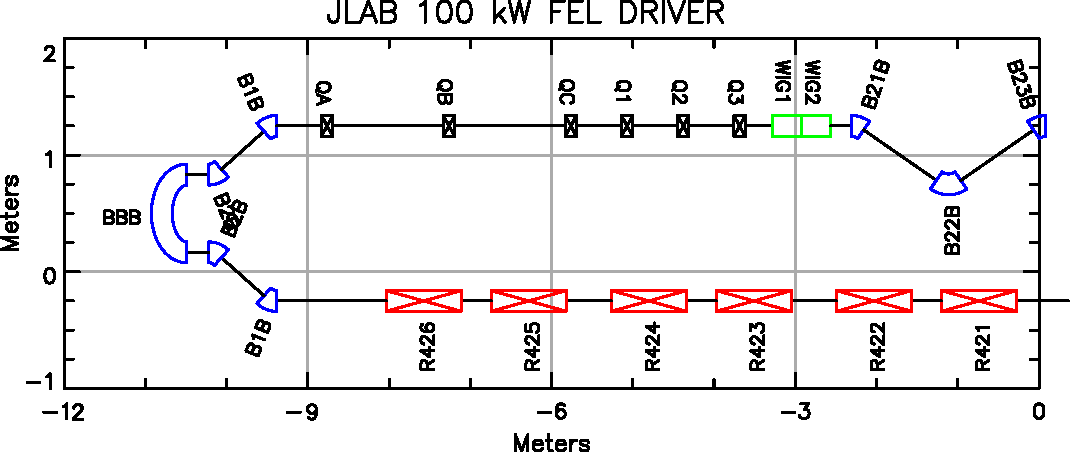
\includegraphics[width=5in]{floor-plan.pdf}
  \caption{Example Floor Plan drawing.}
  \label{f:floor.plan}
\end{figure}

A \vn{floor plan} drawing gives a display of the machine projected onto the horizontal plane.  An
example is shown in Figure~\ref{f:floor.plan}. Like a \vn{Lattice Layout} (\sref{s:lat.layout}),
Elements are represented by colored rectangles and which elements are drawn is determined by a
\vn{floor_plan_drawing} namelist (see~\sref{s:shapes}). Additionally, a cross-section of the walls
of the building containing the machine (\sref{s:building.wall}) can be drawn along with the
reference orbit (which is the closed orbit for machines with a closed geometry). This is illustrated
in Figure~\ref{f:floor.orbit}.

The placement of a lattice element in the drawing is determined by the element's coordinates in the
\vn{global reference system}.  See the Bmad manual for more information on the \vn{global reference
system}.  In the \vn{global reference system}, the $(Z, X)$ plane is the horizontal plane. 

A floor plan orbit is associated with a \vn{graph} of a \vn{plot} (\sref{s:template}). A \vn{graph}
has a \vn{floor_plan} component which is a structure of type \vn{tao_floor_plan_struct}. Components
of this structure can be set to control how a floor plan is drawn. The components of a
\vn{tao_floor_plan_struct} are:
\begin{example}
  type tao_floor_plan_struct
    rotation             = <real>      ! Rotation of floor plan plot: 1.0 -> 360 deg. 
    view                 = "<string>"  ! View plane for floor plan plot. default = "zx"
    correct_distortion   = <logical>   ! For Floor Plan plots: Default = F
    flip_label_side      = <logical>   ! Draw element label on other side of element?
    size_is_absolute     = <logical>   ! Shape sizes scaled to absolute dimensions?
    draw_only_first_pass = <logical>   ! Draw only first pass with multipass elements?
    orbit_scale          = <real>      ! Scale for the orbit. Default = 0 => No orbit drawn.
    orbit_color          = "<color>"   ! Line color. Default = "red".
    orbit_pattern        = "<pattern>" ! Line pattern. Default = "solid_line".
    orbit_width          = <integer>   ! Line width. Default = 1.
  end type
\end{example}
A graph is initialized with a \vn{tao_template_graph} namelist (\sref{s:template}). Example:
\begin{example}
  &tao_template_graph
    ...
    graph%floor_plan%rotation = 0.5  ! Rotate 180 degrees
    graph%floor_plan%orbit_scale = 100
    graph%floor_plan%orbit_color = "red"
    graph%floor_plan%orbit_width = 3
  /
\end{example}

The \vn{scale} component scales the displacement of the orbit from the lattice reference coordinate
system (which is the centerline of the lattice elements if there are no misalignments). So a value
of 100.0, a 1~cm orbit is drawn 1~meter from the centerline. A setting of zero (the default) means
that the orbit is now drawn. Note: If \vn{scale} is not unity, the plotted orbit when going through
a \vn{patch} element with a finite transverse offset will show a discontinuity due to the
discontinuity of the reference orbit.

What plane a floor plan is projected onto is determined by the setting of the
\vn{graph%floor_plan%view} switch. This switch is a two character string.  Each character is either
"x", "y", or "z" and the characters must not be both the same. Default is "zx". The first character
determines which global coordinate is mapped to the horizontal axis of the graph and the second
character determines which global coordinate is mapped to the vertical axis of the graph. There are
six possible two character combinations. The default "zx" setting represents looking at the
horizontal plane from above. A setting of "xz" represents looking at the horizontal plane from
below. The other combinations involving "y" are only potentially useful if the machine has a significant
vertical extent.

%----------------
\begin{figure}[b]
  \centering
  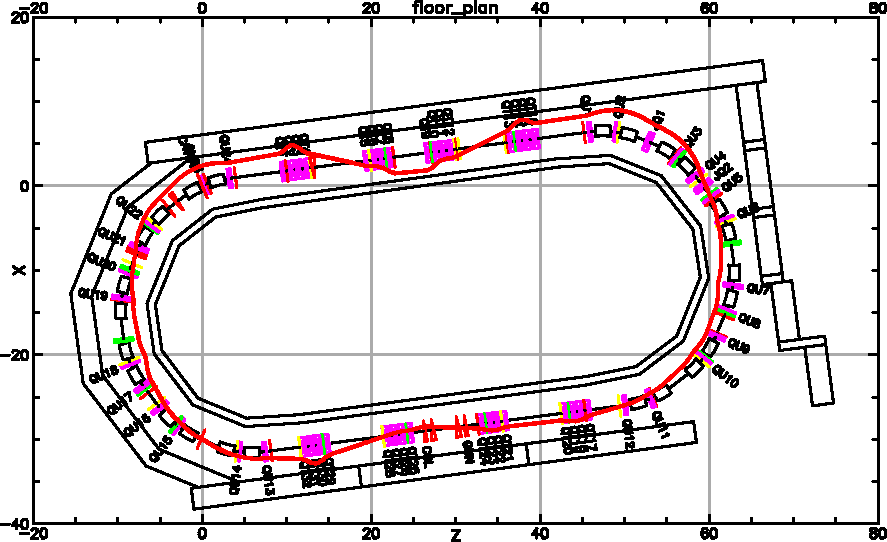
\includegraphics[width=5in]{floor-plan-orbit.pdf}
  \caption[Floor plan with orbit and building walls.]{Example Floor plan drawing with the closed orbit 
(red line) and building walls included.}
  \label{f:floor.orbit}
\end{figure}
%----------------

If element labels are to be drawn, on which side the labels are drawn can be flipped by setting 
\vn{graph%floor_plan%flip_label_side} to True.

The \vn{size_is_absolute} logical is combined with the \vn{<size>} setting for a shape to determine the
size transverse to the center line curve of the drawn shape (\sref{s:shapes}).
If \vn{size_is_absolute} is False (the default), \vn{<size>} is taken to be the size of
the shape in points (72 points is approximately 1 inch). If \vn{size_is_absolute} is True,
\vn{<size>} is taken to be the size in meters. That is, if \vn{size_is_absolute} is
False, zooming in or out will not affect the size of an element shape while if
\vn{size_is_absolute} is True, the size of an element will scale when zooming.

An overall rotation of the floor plan can be controlled by setting \vn{rotation} parameter. A
setting of 1.0 corresponds to 360$^\circ$. Positive values correspond to counter-clockwise
rotations.  Alternatively, the global coordinates at the start of the lattice can be defined in the
lattice file and this can rotate the floor plan.  Unless there is an offset specified in the lattice
file, a lattice will start at $(x, y) = (0, 0)$. Assuming that the machine lies in the horizontal
plane with no negative bends, the reference orbit will start out pointing in the negative $x$
direction and will circle clockwise in the $(x, y)$ plane.

The \vn{draw_only_first_pass} logical, if set True, suppresses drawing of \vn{multipass_slave}
lattice elements that are associated with the second and higher passes. This logical defaults to
False. Setting to True is only useful in some extreme circumstances where the plotting of additional
passes leads to large pdf/ps file sizes.

Note: If \vn{graph%ix_universe} is set to -1 the current viewed universe is used. If
\vn{graph%ix_universe} is set to -2, all universes are plotted.

Example Floor Plan template:
\begin{example}
  &tao_template_plot
    plot%name = "floor"
    plot%x%min = -12  
    plot%x%max = 0    
    plot%x%major_div_nominal = 4
    plot%x%minor_div = 3
    plot%n_graph = 1
  /

  &tao_template_graph
    graph_index = 1
    graph%name = "1"
    graph%type = "floor_plan"
    graph%box = 1, 1, 1, 1
    graph%margin = 0.10, 0.10, 0.10, 0.10, "%BOX"
    graph%ix_universe = -2   ! Draw all universes.
    graph%x%label = "SMART LABEL"
    graph%y%label = "SMART LABEL"
    graph%y%max = 2  
    graph%y%min = -1 
    graph%floor_plan%correct__distortion = T
    graph%floor_plan%size_is_absolute = T
    graph%floor_plan%view = "xz"  ! Looking from beneath
    graph%floor_plan%orbit_scale = 100
  /
\end{example}

Having \vn{graph%x%label} and \vn{graph%y%label} set to ``\vn{SMART LABEL}'' means that the actual axis labels will be 
picked appropriately based upon the setting of \vn{graph%floor_plan%view}.

To prevent the drawing of the axes set \vn{graph%draw_axes} to False.  To prevent the drawing of a
grid at the major division points set \vn{graph%draw_grid} to False.

By default, the horizontal or vertical margins of the graph will be increased so that the horizontal
scale (meters per plotting inch) is equal to the vertical scale.  If
\vn{graph%floor_plan%correct_distortion} is set to \vn{False}, this scaling will not be done.

Note: The \vn{show ele -floor} command (\sref{s:show}) can be used to view an element's global
coordinates.

%-----------------------------------------------------------------
\subsection{Defining Shapes for Lat_layout and Floor_plan Drawings}
\label{s:shapes}
\index{lat_layout drawings}
\index{floor_plan drawings}

\vn{Floor plan} (\sref{s:floor.plan}) and \vn{lattice layout} drawings use various shapes, sizes,
and colors to represent lattice elements. The association of a particular element with a given shape
is determined via two namelists: \vn{lat_layout_drawing} for the lattice layout and
\vn{floor_plan_drawing} for floor plan drawings.  Two different namelists are used since, for
example, a size that is good for a layout will not necessarily be good for a floor plan.

The file that \tao looks in to find these two namelists is set by the first file specified in the
\vn{plot_file} array set in the \vn{tao_start} namelist (\sref{s:init.global}). The default, if
\vn{plot_file} is not set, is the root initialization file.

The namelist syntax is the same for both:
\begin{example}
  &lat_layout_drawing
    include_default_shapes = <logical>
    ele_shape(i) = "<ele_id>" "<shape>" "<color>" "<size>" "<label>" <draw> 
                                                                <multi> <line_width>
  /

  &floor_plan_drawing
    ... same as lat_layout_drawing ...
  /
\end{example}
For Example:
\begin{example}
  &floor_plan_drawing
    include_default_shapes = T
    !               ele_id                  Shape        Color     Size  Label  ..etc..
    ele_shape(1) = "quadrupole::q*"         "box"        "red"     0.75  "name"  
    ele_shape(2) = "quadrupole::*"          "xbox"       "red"     0.75  "none" 
    ele_shape(3) = "sbend::sb*"             "box"        "blue"    0.37  "none"
    ele_shape(4) = "sbend::*"               "box"        "blue"    0.37  "none"  
    ele_shape(5) = "wiggler::*"             "xbox"       "green"   0.50  "name"
    ele_shape(6) = "var::quad_k1"           "circle"     "purple"  0.25  "name"
    ele_shape(7) = "data::orbit.x|design"   "vvar:box"   "orange"  0.25  "name"
    ele_shape(8) = "building_wall::*"       "solid_line" "black"    0    "none"
    ele_shape(3)%multi = T
    ele_shape(5:6)%line_width = 5, 6
  /
\end{example}
A figure is drawn for each lattice element in the lattice that matches the \vn{<ele_id>} field
(\sref{s:ele.list.format}). Thus, in the example above, \vn{ele_shape(1)} will match to all
quadrupoles whose name begins with ``q'' and \vn{ele_shape(2)} will match all quadrupoles.

Besides the usual element class prefixes (\vn{quadrupole::}, \vn{sbend::}, etc.), other prefixes
that can be used with an \vn{<ele_id>} are
\begin{example}
  data::            ! Match to \tao datum name.
  var::             ! Match to \tao variable name.
  alias::           ! Match to lattice element alias parameter.
  type::            ! Match to lattice element type parameter.
  building_wall::   ! Used in floor_plan plots.
\end{example}
The \vn{data::} prefix is used to match to data that will be used in an optimization. Thus, in the
above example, \vn{ele_shape(7)} specifies that an ``x'' will be drawn at points where there is
valid \vn{orbit.x} data. For this to work, an \vn{orbit.x} data array must be defined
(\sref{s:init.data}).

The \vn{var::} prefix is used for drawing variable locations for variables used in an
optimization. In the above example, it is assumed that a \vn{quad_k1} variable array has been
setup. A circle will be drawn at each element under control of a \vn{quad_k1} variable.

For \vn{floor_plan} drawings, the building wall (\sref{s:building.wall}) can be drawn by specifying
an \vn{ele_shape} whose name is \vn{"building_wall::<name>"} where \vn{<name>} is used to match to
the building wall section name. Use ``\vn{*}'' for \vn{<name>} to match to all names. For the
building wall, the only attribute that is relevant is the \vn{<color>} attribute.

The \vn{alias::} and \vn{type::} prefixes for \vn{<ele_id>} are used to match to the \vn{alias} and
\vn{type} string parameters of that can be set in the lattice file for each individual element.

If an element matches more than one shape,
what is drawn depends upon the setting of \vn{<multi>}. If \vn{<multi>} is False (the default) for
the first shape matched in the list of shapes, only this shape will be used.  If \vn{<multi>} is
True, \tao will draw this shape and then look for additional matches. Each time an additional match
is found, the shape is drawn and the setting of \vn{<multi>} for that shape will be used to
determine whether additional shapes are searched for. Thus \vn{<multi>} can be use to draw, for
example, a \vn{circle} shape superimposed upon a \vn{bow_tie} shape.

\tao defines a set of default shapes in case no shapes are defined in the plot file. If the
optional \vn{include_default_shapes} logical, which can be set for either \vn{floor_plan} and/or
\vn{lat_layout} shape namelists, is set to False (the default), the default shapes are not used.
If \vn{include_default_shapes} is set to True, the default shapes are appended to the list of 
shapes.

Use the \vn{show plot -floor_plan} and \vn{show plot -lat_layout} commands to see the defined
shapes. Use the \vn{set floor_plan} and \vn{set lat_layout} commands (\sref{s:set})) to set shape
parameters on the command line.

The width of a drawn shape is the width of the associated element. The exception is the \vn{"x"}
shape whose width is always the same as the height determined by the \vn{<size>} setting.

\vn{<size>} is the half height of the shape. That is, the size transverse to the longitudinal
dimension. For \vn{lat_layout} drawings, \vn{<size>} = 1.0 corresponds to full scale if the default
\vn{graph%y%min} = -1 and \vn{graph%y%max} = 1 are used. For {floor_plan} drawings, the drawn size
is also affected by the setting of \vn{graph%floor_plan%size_is_absolute} See \sref{s:floor.plan}
for more details.

The overall size of all the shapes can be scaled using the \vn{plot_page} (\sref{s:init.plot})
parameters
\begin{example}
  floor_plan_shape_scale     ! For floor_plan drawings. Default = 1
  lat_layout_shape_scale     ! For lat_layout drawings. Default = 1
\end{example}

The text size in both \vn{floor_plan} and \vn{lat_layout}
plots can be scaled by using the \vn{plot_page} parameter
\begin{example}
  legend_text_scale          ! Default = 1
\end{example}
Use the \vn{show plot} command to view these parameters. Use the
\vn{set plot_page} command to set these parameters.

\vn{<color>} is the color of the shape. Good colors to use are:
\index{element shape!color}
\begin{example}
  "black"
  "blue"
  "cyan"
  "green"
  "magenta"
  "orange"
  "purple"
  "red"
  "yellow"
\end{example}

The \vn{<line_width>} parameter is an integer that specifies the width of the lines drawn. The
default is 1.

The \vn{<label>} indicates what type of label to print next to the corresponding
element glyph. Possibilities are:
\begin{example}
  name            -- The element name (default).
  none            -- No label is drawn.
  s               -- Draw longitudinal s position.
\end{example}
The default is \vn{"name"}

The \vn{<draw>} field determines if a shape is drawn or not. The default is \vn{T}. This can be
useful for toggling on and off the drawing of shapes using the \vn{set shape} command
(\sref{s:set}).

Note: There is an old, deprecated syntax where both the lattice layout and floor plan drawings are
specified via one \vn{element_shapes} namelist.

The \vn{<shape>} parameter is the shape of the figure drawn. The \vn{<shape>} string will have the
form:
\begin{example}
  <shape-name>  or
  <prefix>:<shape-name>  
\end{example}
Valid \vn{shape-name}s are: 
\index{box}\index{xbox}
\begin{example}
  "box"            -- Rectangular box
  "bow_tie"        -- Bow-tie shape.
  "circle"         -- Circle centered at center of element.
  "diamond"        -- Diamond shape.
  <pattern_name>   -- Custom shape specified by <name>. Used with "pattern" prefix.
  "rbow_tie"       -- Bow-tie shape rotated 90 degrees.
  "d_triangle"     -- Triangle pointing ``down''.
  "l_triangle"     -- Triangle pointing ``left'' (upstream).
  "r_triangle"     -- Triangle pointing ``right'' (downstream).
  "u_triangle"     -- Triangle pointing ``up''. 
  "x"              -- "X" centered at center of element
  "xbox"           -- Rectangular box with an x through it.
  "dashed_line"    -- Only used with ele_id set to "building_wall".
  "dash_dot_line"  -- Only used with ele_id set to "building_wall".
  "dotted_line"    -- Only used with ele_id set to "building_wall".
  "solid_line"     -- Only used with ele_id set to "building_wall".
\end{example}
Valid prefixes are:
\begin{example}
  "asym_var"   -- Like "var" prefix but is not symmetric about the center line.
  "asym_vvar"  -- Like asym_var except scaled to associated variable or datum.
  "pattern"    -- Custom shape. <shape-name> here is a pattern name.
  "var"        -- Shape with variable height. 
                       The shape size is symmetric about the center line.
  "vvar"       -- Like "var" prefix except scaled to associated variable or datum.
\end{example}

For example, if an element's shape is set to \vn{var:box} or \vn{asym_var:box}, the drawn size of the
element is proportional to the element's magnetic or electric strength. The associated
\vn{<size>} setting is the multiplier used to scale from element strength to height. For
example, for a quadrupole the height is proportional to the \vn{K1} focusing strength. The
difference between \vn{var:box} or \vn{asym_var:box} is that with \vn{var:box} the drawn
box is symmetric with respect to the centerline with a size independent of the sign of the
element strength. On the other hand, with \vn{asym_var:box}, the drawn box will terminate
with one side on the centerline and the side on which it is drawn will depend upon the the
sign of the element strength. Note: Not all lattice elements can be used with a
\vn{var:box} or \vn{asym_var:box}.

A \vn{vvar:box} shape is like a \vn{var:box} and a \vn{asym_vvar:box} is like a
\vn{asym_var:box}. The difference is that \vn{vvar:box} and \vn{asym_vvar:box} shapes may only be
used when the \vn{<ele_id>} is associated with data or variables. That is, when the \vn{<ele_id>}
string starts with ``\vn{data::}'' or ``\vn{var::}''. In this case, the height of the box, instead
of being proportional to the strength of the element, is proportional to the value of the associated
datum or variable. If no datum or variable component is specified in the \vn{ele_id}, the model
value will be used. Thus, in the above example, where \vn{<ele_id>} was set to
\vn{"data::orbit.x|design"}, the design value is used.

The \vn{solid_line}, \vn{dashed_line}, \vn{dash_dot_line}, and \vn{solid_line} settings for
\vn{<shape>} is used when \vn{<ele_id>} is set to \vn{building_wall} to indicate what type of line
is to be drawn.

The \vn{pattern:<pattern_name>} shape allows for a custom pattern to be specified. Custom
patterns are specified by a \vn{shape_pattern} namelist:
\begin{example}
  &shape_pattern
    name = "<curve_name>"
    line%width = <line_width>
    pt(1) = <s>, <x>
    pt(2) = <s>, <x>
    pt(3) = ...
  /
\end{example}
Example:
\begin{example}
  &floor_plan_drawing
    ...
    ele_shape(2) = "quadrupole::*"     "pattern:q_pat"     "red"     0.75     "none" 
    ...
  /

  &shape_pattern
    name = "q_pat"
    pt(1) = 0, -1
    pt(2) = 1, -1
    pt(3) = 0.9, 1
    pt(4) = 0.1, 1
    pt(5) = 0, -1
  /
\end{example}
The \vn{name} of the \vn{shape_pattern} namelist (in this example it is "q_pat") must match the name
given by \vn{"pattern:<pattern_name>"}. The pattern is specified by a number of points. Between the
points, a line segment is drawn. In the above example, the pattern is an isosceles trapezoid.  When
drawn, the \vn{s} coordinate is scaled so that $s = 0$ corresponds to the entrance end of the
element and $s = 1$ corresponds to the exit end. The \vn{x} coordinate is scaled by the \vn{size}
attribute of the \vn{ele_shape}. The color of the line segments is set by the definition and the width
of the line segments is set by the pattern definition.

%-----------------------------------------------------------------
\subsection{Drawing Apertures}
\index{aperture drawing}
\label{s:draw.ap}

\begin{figure}
  \centering
  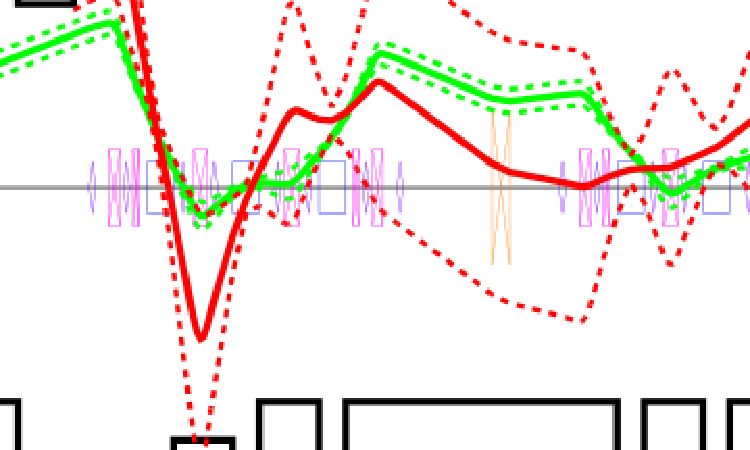
\includegraphics[width=6in]{aperture-plot.pdf}
  \caption[Example beam aperture plot.]
{Example plot of the beam aperture. In this drawing, two turns of three injected particles are drawn. The
particles start at different positions and illustrate what the size of an injected beam would be. Also drawn
(a bit faint) is a \vn{lat_layout} showing lattice element positions.}
  \label{f:aperture}
\end{figure}

Beam apertures can be defined in the \bmad lattice file. Apertures can be defined in one of three
ways. The most common is to set limit or aperture parameters for an element. Another possibility 
is to use a \vn{mask} element (which can be used to define an aperture of arbitrary shape). The
third possibility involves defining a continuous three-dimensional wall. This third possibility 
is only used with Runge-Kutta type tracking. 

To simplify things, the drawing of the beam aperture ignores any \vn{mask} elements (since the
geometry can be very complicated here) and ignores any three-dimensional walls (which are only
used for Runge-Kutta type tracking). \fig{f:aperture} shows an example of a aperture drawing.

To draw an aperture, a curve's \vn{data_source} parameter must be set to \vn{"aperture"} and the \vn{data_type} parameter is set to one of
\begin{example}
  "+x"     ! Aperture in +X direction
  "-x"     ! Aperture in -X direction
  "+y"     ! Aperture in +Y direction
  "-y"     ! Aperture in -Y direction
\end{example}
The apertures in the $+x$ and $+y$ directions will have positive values and the apertures in the
$-x$ and $-y$ directions will have negative values. Set the curve's \vn{y_axis_scale_factor} to scale
tye aperture curve if needed.

The following example will graphs the horizontal orbit along with the horizontal apertures.
\begin{example}
  &tao_template_plot
    plot%name        = "x_orbit"
    plot%x_axis_type = "s"
    plot%n_graph     = 1
  /

  &tao_template_graph
    graph%name    = "x"
    graph_index   = 1
    graph%n_curve = 3

    curve(1)%data_source  = "aperture"
    curve(1)%data_type    = "+x"
    curve(1)%draw_symbols = T
    curve(1)%draw_line    = F
    curve(1)%data_source  = "aperture"
    curve(2)%data_type    = "-x"
    curve(2)%draw_symbols = T
    curve(2)%draw_line    = F
    curve(3)%data_type = "orbit.x"
  /
\end{example}
Note: Aperture curves will ignore the \vn{curve%component} parameter.

%-----------------------------------------------------------------
\subsection{Drawing Dynamic Aperture Curves}
\index{dynamic aperture drawing}
\label{s:dynamic.ap.plot}

A \vn{dynamic_aperture} drawing displays the results of the dynamic aperture
calculation (\sref{s:dynamicaperture}). Example plot setup:
\begin{example}
&tao_template_plot
  plot%name = "da"
  plot%x%min = -20
  plot%x%max =  20
  plot%x%major_div_nominal = 10
  plot%x%label = "x (mm)"
  plot%x_axis_type = "phase_space"
  plot%n_graph = 1
/

&tao_template_graph
  graph%name = "g1"
  graph%type = "dynamic_aperture"
  graph_index = 1
  graph%title = "dynamic aperture"
  graph%margin =  0.15, 0.06, 0.12, 0.12, "%BOX"
  graph%x_axis_scale_factor = 1000
  graph%y%label = "y (mm)"
  graph%y%label_offset = .2
  graph%y%major_div = 4
  graph%n_curve = 3
  curve(1:3)%y_axis_scale_factor = 3*1000
  curve(1:3)%draw_symbols = 3*F
  curve(3)%data_type = "physical_aperture"
  curve(3)%line%color = "red"
  curve(3)%line%width = 5 
/
\end{example}
This produces Fig.~\ref{f:da-plot}.  Each curve represents a single momentum
calculation.  If there are more momenta than curves (as in this case), additional curves will
automatically be created using the styles of the previous curves. Note that apertures are calculated
at element 0.

\begin{figure}
  \centering
  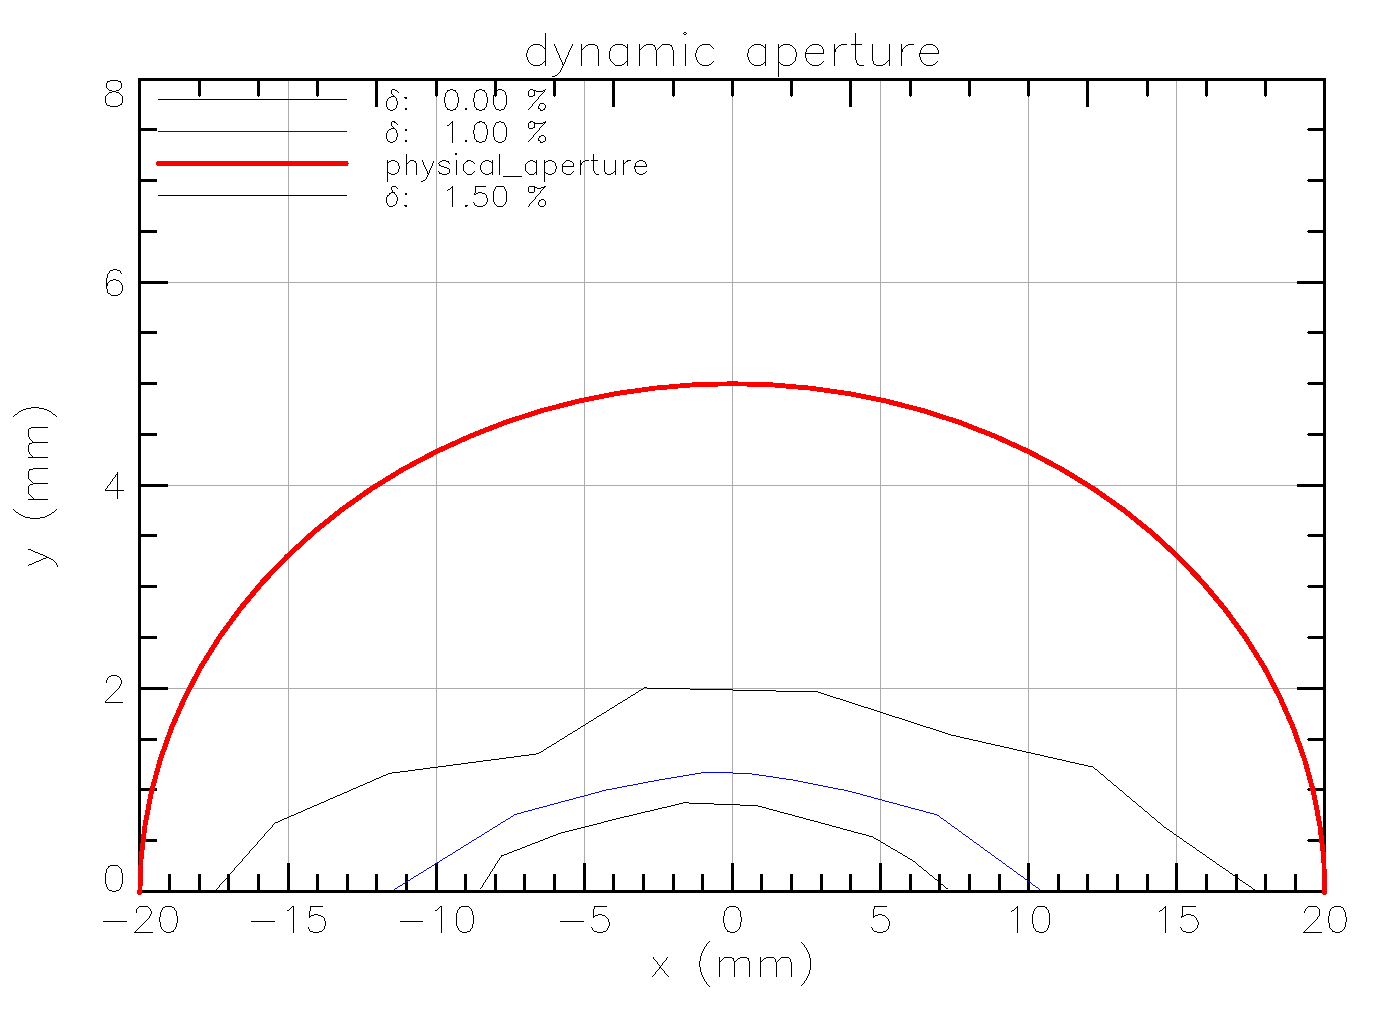
\includegraphics[width=5in]{dynamic-aperture.pdf}
  \caption{Example dynamic aperture plot.}
  \label{f:da-plot}
\end{figure}

If there is a curve with \vn{%data_type} set to \vn{"physical_aperture"}, and if there is a lattice
element at $s = 0$ that has an aperture set, this physical aperture will be drawn. Example: In the
\bmad lattice file define a marker element with an aperture and superimpose the marker at the
beginning of the lattice:
\begin{example}
  m: marker, x_limit = 0.045, y_limit = 0.025, superimpose
\end{example}

Dynamic aperture curves can have the following \vn{%data_type}:
\begin{example}
  "dynamic_aperture" or ""    ! (default) points include the reference orbit
  "dynamic_aperture_centered" ! points are centered (relative to) the reference orbit
  "physical_aperture"         ! draws the physical aperture based on x1_limit, etc. 
\end{example}

%-----------------------------------------------------------------
\subsection{Drawing a Histogram}
\index{histogram drawing}
\label{s:histogram}

A \vn{histogram} drawing displays a histogram of phase space beam density. Histogram plotting is
associated with a \vn{graph} by setting \vn{graph%type} equal to \vn{"histogram"}. The concepts here
are similar to \vn{phase space} plotting (\sref{s:phase.space}). An example is shown in
Fig.~\ref{f:histogram}, using the example histogram template:
\begin{example}
&tao_template_plot
  plot%name = "zhist"
  plot%x%min = -6
  plot%x%max =  6
  plot%x%label = "z (mm)"
  plot%n_graph = 1
/

&tao_template_graph
  graph_index = 1
  graph%name = "z"
  graph%type = "histogram"
  graph%box = 1, 1, 1, 1
  graph%title = "Bunch Histogram: Z"
  graph%margin =  0.15, 0.06, 0.12, 0.12, "%BOX"
  graph%y%label = "Current (A)"
  graph%n_curve = 1
  graph%y%label_offset = .1
  graph%x_axis_scale_factor = 1000.00 !m->mm

  curve(1)%hist%density_normalized = T
  curve(1)%hist%weight_by_charge = T
  curve(1)%hist%number = 100
  curve(1)%line%color = "blue"
  curve(1)%line%pattern = "dashed"
  curve(1)%y_axis_scale_factor = 299792458  !Q/m * c_light
  curve(1)%data_type = "z" 
  curve(1)%data_source = "beam_tracking"
  curve(1)%ele_ref_name = "BEGINNING"
  curve(1)%symbol%type = "dot"
/
\end{example}

\begin{figure}
  \centering
  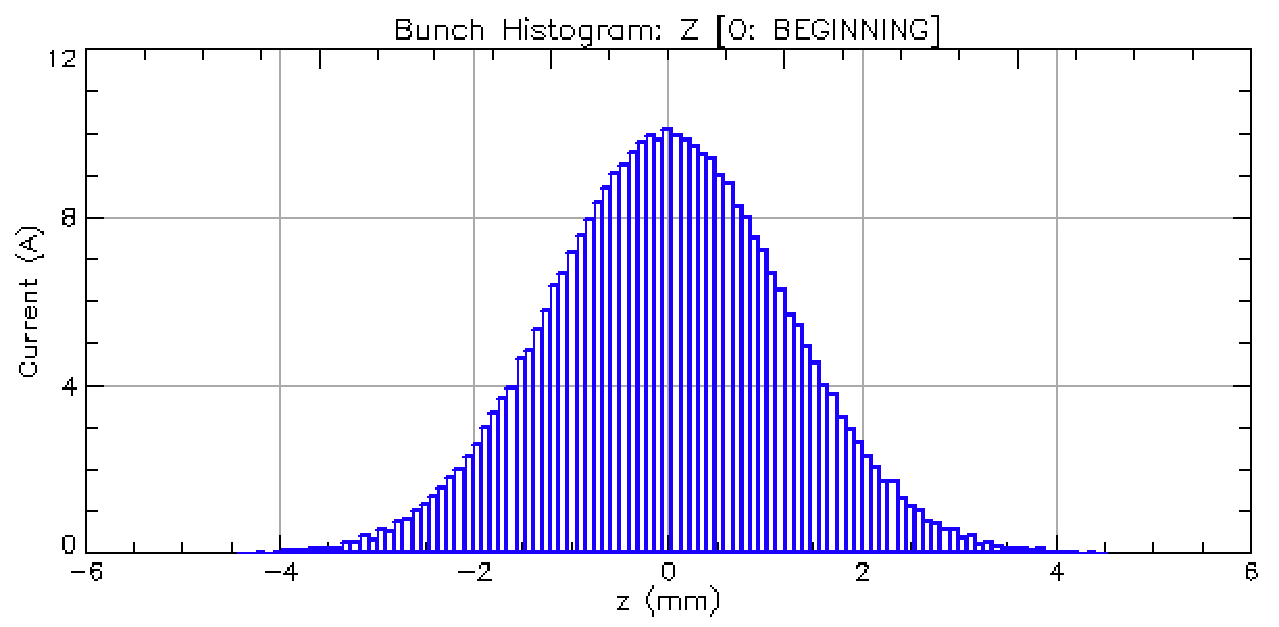
\includegraphics[width=5in]{histogram.pdf}
  \caption{Example histogram plot.}
  \label{f:histogram}
\end{figure}

For a \vn{"histogram"} type graph, \vn{curve%data_type} determines what coordinate is plotted along
the x-axis.  Valid \vn{curve%data_type} values are:
\index{x}\index{px}\index{y}\index{py}\index{z}\index{pz}
\begin{example}
  "x"
  "px"
  "y"
  "py"
  "z"
  "pz"
  "intensity"       -- Photon total intensity 
  "intensity_x"     -- Photon intensity along x-axis 
  "intensity_y"     -- Photon intensity along y-axis
  "phase_x"         -- Photon phase along x-axis
  "phase_y"         -- Photon phase along y-axis
\end{example}
In this example above, the $x$-axis of the plot will correspond to the $z$ phase space coordinate.

The maximum and minimum of the bins is set automatically to fit the data.  The
\vn{curve%hist%number} establishes the number of bins. Alternatively, if \vn{curve%hist%number = 0},
then \vn{curve%hist%width} establishes
 the width of the histogram bins and sets the number automatically. 

If \vn{curve%hist%density_normalized = T}, then the height of a bin will be divided by its width. If
\vn{curve%hist%weight_by_charge = T}, then the particle charge will be used to bin, otherwise the
particle count will be used to bin.

The \vn{curve%hist%center} will insure that a bin will be centered at this location.

\index{curve!ele_ref_name}
To change the place in the lattice where the data for the \vn{histogram} is evaluated, use the
\vn{set curve ele_ref_name} command.

If \vn{graph%type} is \vn{"histogram"} then \vn{curve%data_source} 
must be either:
\begin{example}
  "beam"
  "multi_turn_orbit"
\end{example} 
\vn{"beam"} indicates that the points of the histogram plot will be obtained correspond to the
positions of the particles within a tracked beam. \vn{multi_turn_orbit"} is used for rings where a
single particle is tracked multiple turns and the position of this particle is recorded each
turn. In this case, a \vn{d2_data} structure must have been set up to hold the turn--by--turn
orbit. This \vn{d2_data} structure must be called \vn{multi_turn_orbit} and must have \vn{d1_data}
data arrays for the histogram planes to be plotted. For example, if the histogram plot is \vn{x}
versus \vn{px}, then there must be \vn{d1_data} arrays named \vn{"x"} and \vn{"px"}. The number of
turns is determined by the setting of \vn{ix_max_data} in the \vn{tao_d1_data} namelist
(\sref{s:init.data}).

%%-----------------------------------------------------------------
%\subsection{Drawing the Beam Chamber Wall}
%\index{beam chamber wall}
%\label{s:beam.wall.draw}
%
%If a beam chamber wall has been defined in the lattice file, This wall can be drawn in a \vn{curve}
%by setting \vn{curve%type} to \vn{"beam_chamber_wall"}.
%
%Beam chamber walls are drawn, like a \vn{lat_layout}, on a one dimensional line as a function of
%longitudinal position along the machine centerline.
%
%Note: Use the command \vn{show ele -wall} to print information about the beam chamber wall for a
%particular element.

%%-----------------------------------------------------------------
%\subsection{Drawing Controller Element Curves}
%\index{drawing controller element curves}
%\label{s:draw.control}
%
%A controller element is a \bmad lattice element that controls the parameters of other elements.
%There are three types of controller elements: \vn{groups}, \vn{overlays}, and \vn{rampers}. See 
%the Bmad manual for more details. A controller has one or more independent variables that control
%parameters of other elements. The response of a controlled parameter as a function of any one of 
%controller variables may be plotted.

%% Put under graph%type:
%%  "control_curve"      ! Plot slave response for a controller lattice element (\sref{s:draw.control})


%-----------------------------------------------------------------
\subsection{Drawing a Key Table}
\index{key table}
\label{s:key.table}

The \vn{key table} is explained more fully in Section~\sref{s:key.bind}.  An example is shown in
Figure~\ref{f:layout.table}. A template to create a key table looks like:
\begin{example}
  &tao_template_plot
    plot%name = "table" 
    plot%n_graph = 1
  /

  &tao_template_graph
    graph%type = "key_table" 
    graph_index = 1
    graph%n_curve = 0
  /
\end{example}

The number in the upper left corner, to the left of the first column, (\vn{1} in
Fig.~\ref{f:layout.table}) shows the active \vn{key bank}. The columns in the Key Table are:
\begin{example}
  Ix         ! Key index.
  Name       ! Element name whose attribute is bound.
  Attrib     ! Name of the element attribute that is bound.
  Value      ! Current value of bound attribute.
  Value0     ! Initial value of bound attribute.
  Delta      ! Change in value when the appropriate key is pressed.
  Uni        ! Universe that contains the element.
  Opt        ! Shows if bound attribute is used in an optimization.
\end{example}

Note that in a \vn{Lattice Layout}, if a displayed element has a bound attribute, then the key index
number will be displayed just above the element's glyph.

The \vn{key_table} is drawn with respect to the upper left hand corner of the region in which it is
placed.

%-----------------------------------------------------------------
\subsection{Phase Space Plotting}
\index{phase space plotting}
\label{s:phase.space}

\begin{figure}
  \centering
  \begin{subfigure}[b]{0.45\textwidth}
    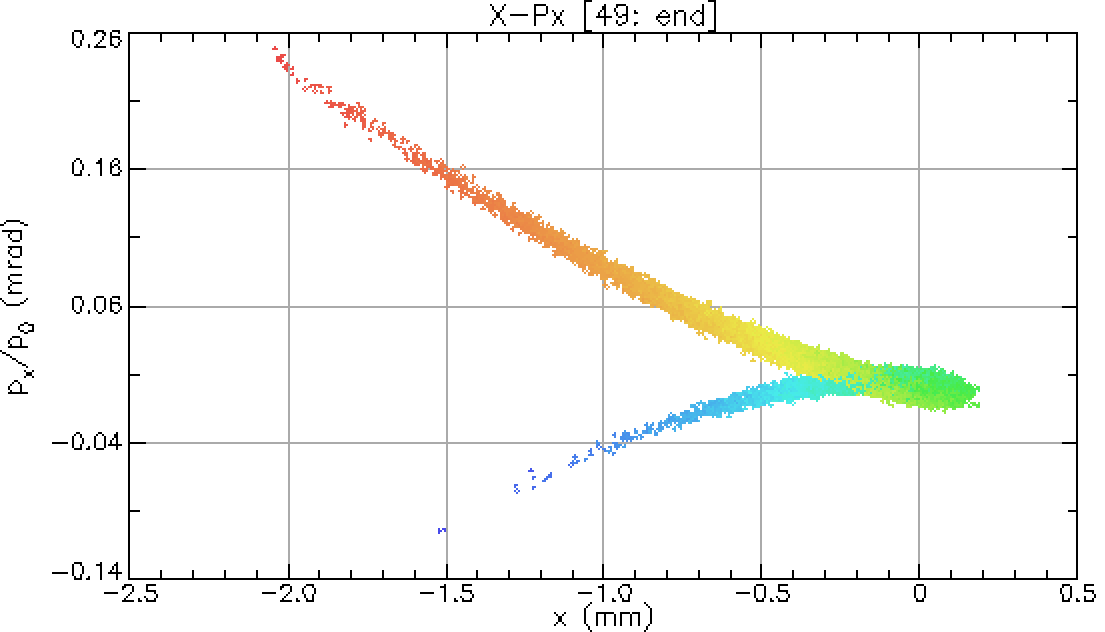
\includegraphics[width=\textwidth]{plot-color-xpx}
    \caption{Horizontal phase space}
  \end{subfigure}
  \begin{subfigure}[b]{0.45\textwidth}
    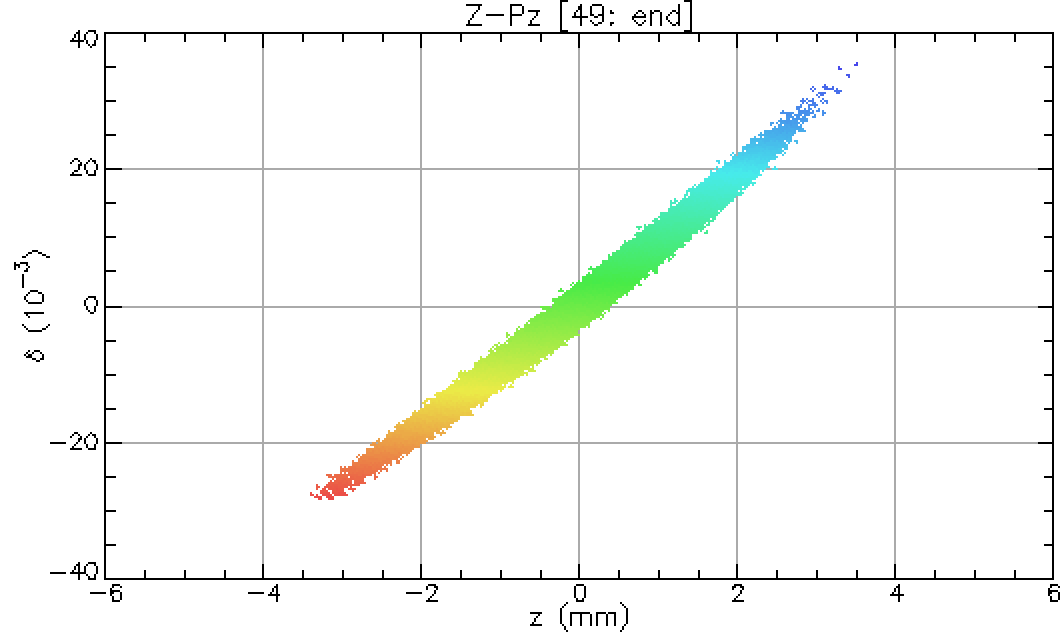
\includegraphics[width=\textwidth]{plot-color-zpz}
    \caption{Longitudinal phase space}
  \end{subfigure}  
  \caption{Example Phase Space plot, with points colored by the \vn{pz} coordinate.}
  \label{f:phase.space}
\end{figure}

A \vn{phase space} plot displays a particle or particles phase space coordinates at a given
location. Phase space plotting is associated with a \vn{graph} by setting \vn{graph%type} equal to
\vn{"phase_space"}. The concepts here are similar to data plotting (\sref{s:plot.data}). An example
is show in Figure~\ref{f:phase.space}.  Example Phase Space template:
\begin{example}
&tao_template_plot
  plot%name = "xphase"
  plot%x%min =   -2.5
  plot%x%max = 0.5
  plot%x%label = "x (mm)"
  plot%n_graph = 1
/

&tao_template_graph
  graph_index = 1
  graph%name = "x"
  graph%type = "phase_space"
  graph%box = 1, 1, 1, 1
  graph%title = "X-Px"
  graph%margin =  0.15, 0.06, 0.12, 0.12, "%BOX"
  graph%x_axis_scale_factor = 1000.00 !m->mm
  graph%y%label =  "p\textbackslash{}dx\textbackslash{}u/p\textbackslash{}d0\textbackslash{}u (mrad)"
  graph%y%major_div = 4
  graph%n_curve = 1
  graph%y%label_offset=.4
  curve(1)%data_type = "x-px" 
  curve(1)%y_axis_scale_factor = 1000 !rad->mrad
  curve(1)%data_source = "beam_tracking"
  curve(1)%ele_ref_name = "END"
  curve(1)%symbol%type = 1
  curve(1)%data_type_z = "pz"
  curve(1)%use_z_color = T
  /
\end{example}

For a \vn{"phase_space"} type graph, \vn{curve%data_type_x} determines what phase space coordinate
is plotted along the x-axis and \vn{curve%data_type} determines what phase space coordinate is
plotted along the y-axis. The phase space coordinates are:
\index{x}\index{px}\index{y}\index{py}\index{z}\index{pz}
\begin{example}
  "x"
  "px"
  "y"
  "py"
  "z"
  "pz"
  "intensity"       -- Photon total intensity 
  "intensity_x"     -- Photon intensity along x-axis 
  "intensity_y"     -- Photon intensity along y-axis
  "phase_x"         -- Photon phase along x-axis
  "phase_y"         -- Photon phase along y-axis
\end{example}
In this example above, the $x$-axis of the plot will correspond to the $z$ phase space coordinate
and the $pz$-axis will correspond to the $px$ coordinate.

\index{curve!ele_ref_name}
To change the place in the lattice where the data for the \vn{phase_space} curve is evaluated, use
the \vn{set curve ele_ref_name} command.

Points can be colored by another phase space coordinate by activating \vn{use_z_color = T}.  The
available curve options and defaults are:
\begin{example}
  use_z_color = F
  data_type_z = "" 
  z_color0 = 0
  z_color1 = 0
  autoscale_z_color = T
\end{example}
These can be the init file, or in Tao using the \vn{set curve} command.  The \vn{data_type_z} can be
set to any of the available phase space coordinates.  \vn{z_color0} and \vn{z_color1} specify the
minimum and maximum of this coordinate to be used in the color range. Values above or below this
range will be colored Black or Grey, respectively.  If \vn{autoscale_z_color=T}, then these will be
set automatically based on the limits of the \vn{data_type_z} coordinate.

If \vn{graph%type} is \vn{"phase_space"} then \vn{curve%data_source} 
must be either:
\begin{example}
  "beam"
  "multi_turn_orbit"
  "twiss"
\end{example} 
\vn{"beam"} indicates that the points of the phase space plot will be obtained correspond to the
positions of the particles within a tracked beam. \vn{multi_turn_orbit"} is used for rings where a
single particle is tracked multiple turns and the position of this particle is recorded each
turn. In this case, a \vn{d2_data} structure must have been set up to hold the turn--by--turn
orbit. This \vn{d2_data} structure must be called \vn{multi_turn_orbit} and must have \vn{d1_data}
data arrays for the phase space planes to be plotted. For example, if the phase space plot is \vn{x}
versus \vn{px}, then there must be \vn{d1_data} arrays named \vn{"x"} and \vn{"px"}. The number of
turns is determined by the setting of \vn{ix_max_data} in the \vn{tao_d1_data} namelist
(\sref{s:init.data}). Using \vn{"twiss"} as the \vn{curve%data_source} indicates that the phase
space plot will be an ellipse whose shape is based upon the Twiss and coupling parameters, and the
normal mode emittances. If the normal mode emittances have not been computed then a nominal value of
1e-6~m-rad is used.

%-----------------------------------------------------------------
\subsection{Parametric Plotting}
\label{s:param.plot}

With parametric plotting, both the $x$ and the $y$ values of the points on a curve are dependent
upon an independent parameter. An example could be plotting $\alpha_a(s)$ versus $\sqrt{\beta_b(s)}$ over
some range of the independent parameter $s$. One way to do parametric plotting is to use data slices
as discussed in section~\sref{s:graph.data.slice}. Another way to do parametric plotting, which is
discussed in this section, is to setup two plot curves whose $y$ values are the desired dependent
parameters ($\alpha_x(s)$ and $\beta_y(s)$ say) and then define a parametric curve which uses the
data from these curves.

The two curves from which the data is to be taken must be in the same graph. The $y$ values from the
first curve will be taken to define the $x$ coordinate of the parametric curve and the $y$ values
from the second curve will be taken to define the $y$ coordinate of the parametric curve. The plot
that holds these curves will be called the ``\vn{source}'' plot. Example:
\begin{example}
  &tao_template_plot
   plot%name = "src"
   plot%x_axis_type = "s"
   plot%n_graph = 1
  /

  &tao_template_graph
   graph_index = 1
   graph%name = "g"
   graph%n_curve = 2
   curve(1)%data_source = "lat"
   curve(1)%data_type = "alpha.a"
   curve(2)%data_source = "lat"
   curve(2)%data_type = "expression: sqrt(beta.b)"
\end{example}
This defines a source plot called \vn{src} with two curves which will be used in the parametric plot. 

The parametric plot curve references the source curves by setting the parametric curve's
\vn{data_source} parameter equal to \vn{"curve"} and the parametric curve's \vn{data_type} to the
graph in the source plot which contains the source curves. For example:
\begin{example}
  &tao_template_plot
    plot%name = "parametric"
    plot%n_graph = 1
    plot%x_axis_type = "curve"
  /

  &tao_template_graph
    graph_index = 1
    graph%name = "g1"
    graph%n_curve = 1
    curve(1)%data_source = "curve"
    curve(1)%data_type = "src.g"
  /
\end{example}
The parametric plot's \vn{x_axis_type} needs to be set to \vn{"curve"} along with the parametric
curve's \vn{data_source}.

When the parametric plot is \vn{placed} in the plot window, \tao will look for a suitable source
plot to connect with. If \tao does not find a suitable source plot, \tao will place a source plot in
an unused plot \vn{region} and set the plot to be invisible. The region name will be set to
\begin{example}
  <source-plot-name>_<parametric-plot-region>
\end{example}
where \vn{<source-plot-name>} is the name of the source plot and \vn{<parametric-plot-region>} is
the name of the region where the parametric plot has been placed. For example, if the above
parametric plot is placed in a region called ``\vn{r12}'', the name of the region where the source
plot is placed will be named ``\vn{src_r12}''. Note: The \vn{show plot} command will show if a plot
in a given region is visible. The \vn{set plot} (\sref{s:set.plot}) command can be used to toggle 
plot visibility.

%-----------------------------------------------------------------
\subsection{QuickPlot Plotting}
\label{s:line.symb}

\vn{QuickPlot} is an interface library developed for \bmad for graphics plotting. QuickPlot uses
the following concepts:
\begin{example}
  PAGE  -- The entire drawing surface.
  BOX   -- The area that the graph with axes, titles, etc. is placed into.
  GRAPH -- The actual plotting area within the bounds of the axes.
\end{example}

For text that has an associated \vn{justify} parameter, the \vn{justify} parameter is a two
character string.  The first character gives the horizontal justification:
\begin{example}
   "L" -- Left justify
   "C" -- Center justify
   "R" -- Right justify
\end{example}
The second character gives the vertical justification
\begin{example}
   "B" -- Bottom justify
   "C" -- Center justify
   "T" -- Top justify
\end{example}

For text that has an associated \vn{units} parameter, the \vn{units} parameter is a character string
which is divided up into three parts. The syntax of the \vn{units} parameter is:
\begin{example}
   "unit_type/ref_object/corner"
\end{example}
Where \vn{unit_type} is the type of units:
\begin{example}
   "%"       - Percent.
   "DATA"    - Data units.
   "MM"      - millimeters.
   "INCH"    - Inches.
   "POINTS"  - Printers points (72 points = 1 inch, 1 pt ~ 1 pixel).
\end{example}
\vn{ref_object} is a reference object (optional except if \vn{unit_type} = "\%").
\begin{example}
   "PAGE"  -- Relative to the page.
   "BOX"   -- Relative to the box.
   "GRAPH" -- Relative to the graph.
\end{example}
And \vn{corner} is the origin location (optional):
\begin{example}
   "LB" -- Left Bottom.
   "LT" -- Left Top.
   "RB" -- Right Bottom.
   "RT" -- Right Top.
\end{example}

\vn{QuickPlot} defines a number of structures to parameterize such things like line and symbol
properties. The structures that \tao uses are as follows.

The \vn{qp_axis_struct} structure defines the properties of a graph axis
\begin{example}
  type qp_axis_struct
    label             = "<string>" ! Axis label string.
    min               = <real>     ! Min is the left or bottom axis number.
    max               = <real>     ! Max is the right or top axis number.
    number_offset     = <real>     ! Offset from axis line in inches.
    label_offset      = <real>     ! Offset from numbers in inches.
    major_tick_len    = <real>     ! Major tick length in inches.
    minor_tick_len    = <real>     ! Minor tick length in inches.
    label_color       = <string>   ! Color of the label string
    major_div         = <integer>  ! Number of major divisions
    major_div_nominal = <integer>  ! Major divisions nominal value.
    minor_div         = <integer>  ! Minor divisions. 0 = Tao will choose.
    minor_div_max     = <integer>  ! Max minor div number if Tao chooses.
    places            = <integer>  ! Number of digits to print
    type              = <string>   ! Axis type: "LINEAR" or "LOG".
    bounds            = <string>   ! Axis bounds: "GENERAL", "ZERO_AT_END", etc.
    tick_side         = <integer>  ! 1 = draw to the inside, 0 = both, -1 = outside.
    number_side       = <integer>  ! 1 = draw to the inside, -1 = outside.
    draw_label        = <logical>  ! Draw the label string
    draw_numbers      = <logical>  ! Draw the numbers.
  end type
\end{example}

The \vn{%bounds} parameter sets how the axes min and max values are calculated.
Possible settings are:
\begin{example}
  "ZERO_AT_END"      ! Min or max value is set to zero.
  "ZERO_SYMMETRIC"   ! Min and max chosen so that max = -min.
  "GENERAL"          ! No restrictions.
  "EXACT"            ! The User min/max is used.
\end{example}
Example \tao session:
\begin{example}
Tao> set graph r13 y%bounds = "zero_at_end"
Tao> scale r13 200 280   ! Graph bounds set to [0, 300]

Tao> set graph r13 y%bounds = "zero_symmetric"
Tao> scale r13 200 280   ! Graph bounds set to [-300, 300]

Tao> set graph r13 y%bounds = "general"
Tao> scale r13 20 190    ! Graph bounds set to [0, 200]

Tao> set graph r13 y%bounds = "exact"
Tao> scale r13 20 190    ! Graph bounds set to [20, 190]
\end{example}

\begin{table}
\begin{tabular}{ll} \toprule
{\B}u       & Start a superscript or end a subscript \\[0.3ex]
{\B}d       & Start a subscript or end a superscript.
              {\B}u and {\B}d must always be used in pairs \\[0.3ex]
{\B}b       & Backspace (i.e., do not advance text pointer  
               after plotting the previous character) \\[0.3ex]
{\B}fn      & Switch to Normal font (1)       \\[0.3ex]
{\B}fr      & Switch to Roman font (2)        \\[0.3ex]
{\B}fi      & Switch to Italic font (3)       \\[0.3ex]
{\B}fs      & Switch to Script font (4)       \\[0.3ex]
{\B}{\B}    & Backslash character (\B)        \\[0.3ex]
{\B}x       & Multiplication sign ($\times$)  \\[0.3ex]
{\B}.       & Centered dot ($\cdot$)          \\[0.3ex]
{\B}A       & Angstrom symbol (\AA)         \\[0.3ex]
{\B}gx      & Greek letter corresponding to roman letter x. See Table~\ref{t:greek}. \\[0.3ex]
{\B}mN {\B}mNN & Graph marker number \vn{N} or \vn{NN} (1-31) \\[1ex]
{\B}(NNNN)  & 
\parbox{5.2in} {Character number NNNN (1 to 4 decimal digits) from the Hershey character set which
includes a number of special characters including mathematical, musical, astronomical, and
cartographical symbols.} \\ \bottomrule
\end{tabular}
\caption{Escape Sequences for Labels.}
\label{t:plot.escape}
\end{table}

The \vn{major_div} parameter is not settable directly. Rather, \vn{major_div_nominal} may be set by
the user and then \tao will calculate the value of \vn{major_div} such that the value of
\vn{major_div} is ``close'' to the value of \vn{major_div_nominal} with the constraint that the value
of \vn{major_div} ``nicely'' divides the range from given by the values for \vn{min} and \vn{max}.

The \vn{places} parameter set the number of places to display a number. \tao will automatically
calculate this number and it is not user settable.

The \vn{label} parameter may include Greek letters, subscripts, superscripts, and special characters.
Encoding for these are given in Table~\ref{t:plot.escape}. 

The \vn{label_color} parameter sets the color of the label string. Possible settings for the color are:
\begin{example}
  White   (actually the background color)       Orange          
  Black   (actually the foreground color)       Yellow_Green    
  Red                                           Light_Green         
  Green                                         Navy_Blue       
  Blue                                          Purple          
  Cyan                                          Reddish_Purple  
  Magenta                                       Dark_Grey        
  Yellow                                        Light_Grey       
\end{example}
Color names are case insensitive.

Table~\ref{t:greek} shows how the character string \vn{"{\B}g<r>"}, where \vn{"<r>"} 
is a Roman letter, map onto the Greek character set.
\begin{table}
  \centering
  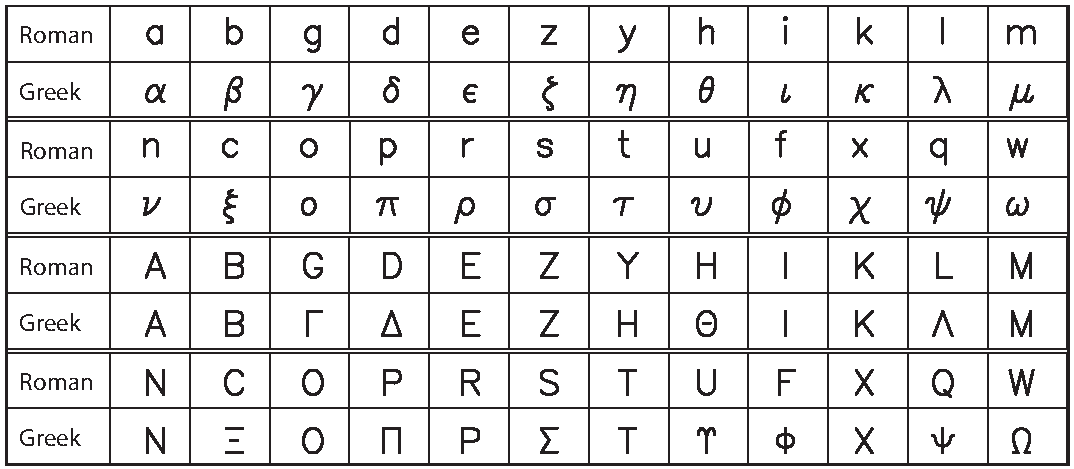
\includegraphics[width=5.0in]{greek.pdf}
  \caption[Roman to Greek Character Conversion]{Conversion for the string 
\vn{"{\B}g<r>"} where \vn{"<r>"} is a Roman character to the corresponding 
Greek character.}
\label{t:greek}
\end{table}

The parameters associated with data lines drawn in a graph are contained in the \vn{qp_line_struct}:
\begin{example}
  type qp_line_struct
    width          = <integer>  ! Default = 1
    color          = <string>   ! Default = "black"
    pattern        = <string>   ! Default = "solid"
  end type
\end{example}

The possible colors for a line are given above. The \vn{pattern} parameter sets how the line is
drawn. Possible settings are:
\begin{example}
  solid      ! Solid line                 dotted     ! Dotted line             
  dashed     ! Dashed line                dash_dot3  ! Dash--dot--dot--dot line
  dash_dot   ! Dash--dot line
\end{example}
Pattern names are case insensitive.

The parameters associated with symbols that are drawn are contained in the \vn{qp_symbol_struct}:
\begin{example}
  type qp_symbol_struct
    type          = <string>  ! Default = "dot"
    height        = <real>    ! Size in points. Default = 10
    color         = <string>  ! Default = "black"
    fill_pattern  = <string>  ! Default = "solid_fill"
    line_width    = <integer> ! Default = 1.
  end type
\end{example}

Possible \vn{fill_pattern} settings are:
\begin{example}
  solid_fill                    hatched           
  no_fill                       cross_hatched     
\end{example}
Fill pattern names are case insensitive.

The symbol types are:
\begin{example}
  square                 triangle                    square_concave              
  dot                    circle_plus                 diamond                     
  plus                   circle_dot                  star5                       
  times                  square_filled               triangle_filled           
  circle                 circle_filled               red_cross                 
  x                      star5_filled                star_of_david             
\end{example}
These symbols are illustrated in Table~\ref{t:plot.syms}. Symbol type names are case insensitive.

\begin{table}
  \centering
  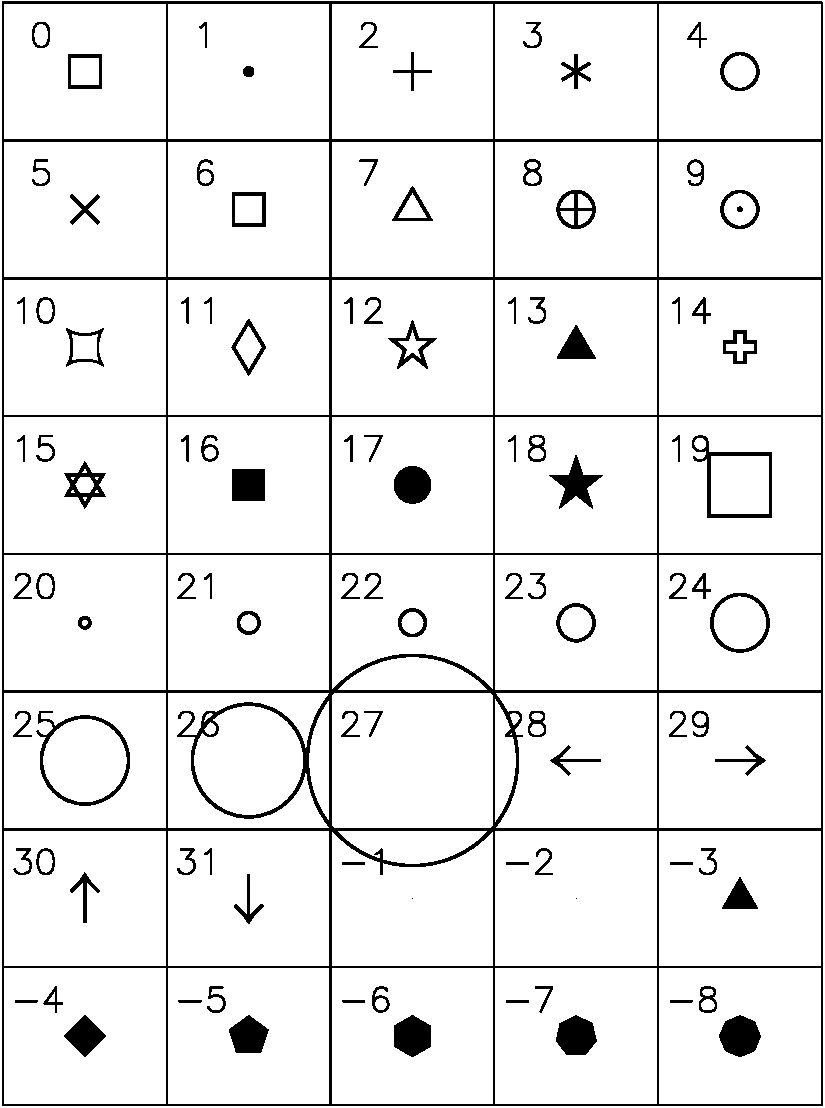
\includegraphics[width=5in]{plot-syms.pdf}
  \caption{Plotting Symbols.}
  \label{t:plot.syms}
\end{table}

%---------------------------------------------------------------------------------------------------------------
%---------------------------------------------------------------------------------------------------------------
% WARNING! If you are modifying this file, be aware that the online help system depends upon the lines starting 
% with "%%" to match blocks of text in this file with a given command. 
%
% The online help system also makes some further assumptions about how this file is formatted.
% Please test any modifications by running Tao and using the appropriate help command to see how
% your modifications translate. 
% Note: The translation code is at: 
%     tao/code/tao_help.f90
%---------------------------------------------------------------------------------------------------------------
%---------------------------------------------------------------------------------------------------------------

\chapter{Commands}
\label{c:command}
\index{commands!Command list} 

\tao has two \vn{modes} for entering commands. In \vn{line mode}'', described in this chapter, \tao
waits until the \vn{return} key is depressed to execute a command. That is, a command consists of a
single line of input. Conversely, \vn{Single Mode}, which is described in \vn{Single Mode} chapter
(\sref{c:single}), interprets each keystroke as a command. Single Mode is useful for quickly varying
parameters to see how they affect a lattice but the number of commands in Single Mode is limited. To
put \tao into \vn{single mode} use the \vn{single_mode} command (\sref{s:sing}).

The syntax for \vn{line mode} commands is discussed in Section~\sref{s:com.syntax}. The list of
commands is shown in Table~\ref{t:commands}.

This chapter uses the following special characters to define the command line syntax:
\begin{example}
  \{\}        ! Identifies an optional argument.
            !   Arguments now enclosed in brackets are required
  <>        ! Indicates a non-literal argument.
\end{example}

Example:
\begin{example}
  change \{-silent\} variable <name>[<locations>] <number>
\end{example}
Here the \vn{-silent} argument is optional while the \vn{variable} argument is mandatory.
Appropriate values for \vn{<name>}, \vn{<locations>}, and \vn{<number>} must be substituted. A
possible

\begin{example}
  change var steering[34:36] @1e-3  ! set the steering strength #34-36 to 0.001
\end{example}

%% command_table -----------------------------------------------------

\begin{table}[h]
\centering {\tt
\begin{tabular}{ll|ll} \toprule
  {\it Command} & {\it Section}     & {\it Command} & {\it Section}     \\ \midrule
  alias         & \sref{s:alias}    & re_execute    & \sref{s:re.exe}   \\
  call          & \sref{s:call}     & read          & \sref{s:read}     \\
  change        & \sref{s:change}   & reinitialize  & \sref{s:reinit}   \\ 
  clear         & \sref{s:clear}    & restore       & \sref{s:restore}  \\ 
  clip          & \sref{s:clip}     & run_optimizer & \sref{s:run}      \\ 
  cut_ring      & \sref{s:cut.ring} & scale         & \sref{s:scale}    \\ 
  continue      & \sref{s:continue} & set           & \sref{s:set}      \\  
  derivative    & \sref{s:deriv}    & show          & \sref{s:show}     \\ 
  do, enddo     & \sref{s:do}       & single_mode   & \sref{s:sing}     \\ 
  end_file      & \sref{s:end.file} & spawn         & \sref{s:spawn}    \\ 
  exit          & \sref{s:exit}     & taper         & \sref{s:taper}    \\
  flatten       & \sref{s:flatten}  & timer         & \sref{s:timer}    \\
  help          & \sref{s:help}     & use           & \sref{s:use}      \\ 
  ls            & \sref{s:ls}       & veto          & \sref{s:veto}     \\ 
  misalign      & \sref{s:misalign} & view          & \sref{s:view}     \\
  pause         & \sref{s:pause}    & wave          & \sref{s:wave}     \\
  place         & \sref{s:place}    & write         & \sref{s:write}    \\ 
  ptc           & \sref{s:ptc}      & x_axis        & \sref{s:x.axis}   \\ 
  python        & \sref{s:python}   & x_scale       & \sref{s:x.scale}  \\ 
  quit          & \sref{s:quit}     & xy_scale      & \sref{s:xy.scale} \\
\bottomrule 
\end{tabular}}
\caption{Table of \tao commands.}
\label{t:commands}
\end{table}

When running \tao, use the \vn{help} (\sref{s:help}) command to show documentation on any command.
For example, \vn{help plot} will show documentation on the \vn{plot} command.

%% Marker: "help" will not display anything after this  -----------

\vfil
\break

%% alias --------------------------------------------------------------
\section{alias}\index{commands!alias}
\label{s:alias}

The \vn{alias} command defines command shortcuts. Format:
\begin{example}
  alias \{<alias_name> <string>\}
\end{example}

\vskip 7pt 

\vn{Alias} is like Unix aliases. Using the \vn{alias} command without any arguments
results in a printout of the aliases that have been defined. When using an alias up to 9 arguments
may be substituted in the \vn{<string>}. The i\Th argument is substituted in place of the sub-string
``[[i]]'' or ``[<i>]''.  Arguments that do not have a corresponding ``[[i]]'' or ``[<i>]'' are
placed at the end of \vn{<string>}. The difference between ``[[i]]'' and ``[<i>]'' is that ``[[i]]''
is a required argument while ``[<i>]'' defines an optional argument. For example
\begin{example}
  alias aaa show element [[1]] [[2]]
  alias zzz show element [[1]] [<2>]
\end{example}
This defines ``\vn{aaa}'' as an alias for the \vn{show element} command with two required arguments
while ``\vn{zzz}'' has only one requred argument.

Aliases can be set up for multiple commands using semicolons.

Examples:
\begin{example}
  alias xyzzy plot [[1]] model  ! Define xyzzy
  alias                         ! Show all aliases
  xyzzy top                     ! Use an alias
  plot top model                ! Equivalent to "xyzzy top"
  xyzzy top abc                 ! Equivalent to "plot top model abc"
  alias foo  show uni; show top ! "foo" equivalent to "show uni; show top"
\end{example}
In the above example ``xyzzy'' is the alias for the string ``plot [[1]] model''.  When the
command xyzzy is used ``top'' is substituted for ``[[1]]'' in the string.

%% call --------------------------------------------------------------
\section{call}\index{commands!call}
\label{s:call}

The \vn{call} command opens a command file (\sref{s:command.files}) and executes the commands in
it. Format: 
\vskip 1pt
\begin{example}
  call <filename> \{<arg_list>\}
  call -no_calc \{<arg_list>\}
  call -ptc <filename>
\end{example}

\vskip 1pt 
The \vn{call} command without \vn{-ptc} is for running a set of \tao commands.  Up to 9
arguments may be passed to the command file. The i\Th argument is substituted in place of the string
``[[i]]'' in the file. Nesting of command files (command files calling other command files) is
allowed. There is no limit to the number of nested files.  See the \vn{Command Files and Aliases}
section (\sref{s:command.files}) for more details.

The \vn{call -ptc} command passes the command file to PTC for processing. Previous to such a call,
the command \vn{ptc init} must be issued. This is for PTC wizards only.

If a command file calls another command file, and the name of the second command file has a relative
(as opposed to absolute) path name, \tao will look for the second command file relative to the
directory of the first command file. To have \tao look relative to your current working directory
(where you started \tao), use the prefix \vn{\$PWD/}. For example, to call a command file that is
one level up from your current working directory use
\begin{example}
  call \$PWD/../second.cmd
\end{example}

Command loops can be implemented in a command file. See the documentation on \vn{do/enddo}
(\sref{s:do}) for more details.

The \vn{-no_calc} option is equivalent to putting the following at the beginning of the
command file to speed up execution time:
\begin{example}
  set global lattice_calc_on = F   ! Stop lattice calculations (\sref{s:lat.calc}).
  set global plot_on = F           ! Halt replotting 
or
  set calc -on                     ! Same as the two lines above.
\end{example}
When using the \vn{-no_calc} option, at the end of the command file the \vn{lattice_calc_on} and
\vn{plot_on} logicals will be toggled back to their initial values.

To suppress the output when running a command file use the command:
\begin{example}
  set global quiet = all
\end{example}
Note: quiet mode is automatically turned off at the end when a command file exits back to the
terminal level. See the \vn{Tao_global_struct Structure} section (\sref{s:tao.global.struct}) for
more details.

Examples:
\begin{example}
    call -no my_cmd_file abc def 
\end{example}
In the above example the argument ``abc'' is substituted for any ``[[1]]'' appearing the
file and ``def'' is substituted for any ``[[2]]''.  \Newline

%% change * --------------------------------------------------------------
\section{change}\index{commands!change}
\label{s:change}

The \vn{change} command changes element attribute values or variable values in the \vn{model}
lattice. Format:
\begin{example}
  change \{-update\} element <element_list> <attribute> \{prefix>\} <number>
  change \{-silent\} variable <name>[<locations>] \{<prefix>\} <number>
  change \{n@\}particle_start <coordinate> \{prefix>\} <number>
  change \{-branch <branch_list>\} \{-listing\} \{-mask <veto_list>\} tune \{dQa\} \{dQb\}
  change \{-branch <branch_list>\} z_tune dQz
\end{example}

\vskip 10pt 
The \vn{change} is used for changing real (as opposed to integer or logical) parameters. Also
consider using the \vn{set} command (\sref{s:set}) which is more general.

If \vn{<prefix>} is not present, \vn{<number>} is added to the existing value
of the attribute or variable. That is:
\begin{example}
  final_model_value = initial_model_value + <number>
\end{example}
If \vn{<prefix>} is present, it may be one of
\begin{example}
  @       final_model_value = <number>
  d       final_model_value = design_value + <number>
  \%       final_model_value = initial_model_value * (1 + <number> / 100)
\end{example}

Element list format (\sref{s:ele.list.format}), without any embedded blanks, is used for
the \vn{<element_list>} argument.

For \vn{change particle_start}, The optional \vn{n@} universe specification (\sref{s:universe}) may
be used to specify the universe or universes to apply the change command to.

For lattices with an open geometry, \vn{change particle_start <coordinate> <number>} can be used to
vary the starting coordinates for single particle tracking. If the \vn{use_particle_start} of the
\vn{beam_init} structure (\sref{s:beam.init}) is set to True, \vn{particle_start} will also vary the
beam centroid and the beam particle spin for tracking. Here \vn{<coordinate>} is one of:
\begin{example}
  x, px, y, py, z, pz, t
\end{example}
For photons, \vn{<coordinate>} may also be:
\begin{example}
  e_photon, field_x, field_y, phase_x, phase_y
\end{example}
For closed lattices only the \vn{pz} component is applicable. For lattices that have an \vn{e_gun}
(which necessarily implies that the lattice has an open geometry), the time \vn{t} coordinate must
be varied instead of \vn{pz}.

For open lattices, \vn{change element beginning <twiss>} can be used to vary the starting Twiss
parameters where \vn{<twiss>} is one of:
\begin{example}
  beta_a, beta_b, alpha_a, alpha_b 
  eta_a, eta_b,etap_a, etap_b    
\end{example}

The \vn{change z_tune} command will vary the longitudinal tune by \vn{<dQz>}. The \vn{<branch_list>}
is used to select which lattice branches the tune is varied in. Each branch listed can have an
optional universe prefix. The default is to vary branch 0 of the current default universe.

The \vn{change tune} command will vary the transverse tunes by \vn{<dQa>} and \vn{<dQb>} and 
the \vn{change z_tune} command will vary the longitudinal tune by \vn{<dQz>}. Units are in radians/2pi
With the \vn{change tune} command, if \vn{<dQa>} or \vn{<dQb>} is not given, the value will
be taken to be zero (that is, no change). The \vn{<branch_list>} is a list of lattice
branches with optional universe prefix, to vary the tunes. The \vn{<veto_list>} of the \vn{-mask}
option gives a list of quadrupoles {\em not} to use for varying the tune. See the \vn{set tune}
(\sref{s:set.tune}) command for more details. The \vn{-listing} option, if present, will, in
addition to the tune change, generate a list of quadrupoles varied along with variation
coefficients.

The \vn{-silent} switch, if present, suppresses the printing of what variables are changed.

The \vn{-update} switch, if present, suppresses \tao from printing error messages if a ``variable
slave value mismatch'' is detected (\sref{s:var.mismatch}). Independent of whether \vn{-update} is
present or not, \tao will fix the mismatch using the changed value to set all of the slave values.

Note: The \vn{change element} command can be used with \vn{ramper} type elements.

Examples:
\begin{example}
  change ele 3@124 x_offset 0.1        ! Offset element #124 in universe 3 by 0.1
  change ele 1,3:5 x_offset 0.1        ! Offset elements 1, 3, 4, and 5 by 0.1
  change ele q* k1 d 1.2e-2            ! Set the k1 strength of all elements starting with
                                       !   the letter "q" relative to the design
  change ele quadrupole::* k1 d 1.2e-2 ! Set the k1 strength of all quadrupole elements.
  change var steering[34:36] @1e-3     ! set the steering strength #34-36 to 0.001
  change var steering[*] \%10           ! vary all steering strengths by 10\%
  change 2@particle_start x @0.001     ! set beginning x position in universe 2 to 1 mm.
  change -mask Q1* tune 0 0.01         ! Change transverse tunes without using quadrupoles
                                       !   whose names start with "Q1".
  change -branch 2@1 z_tune 0.02       ! Change z-tune of branch #1 of universe #2.
\end{example}


%% clear --------------------------------------------------------------
\section{clear}\index{commands!clear}
\label{s:clear}

The \vn{clear} command clears stored spin and orbital Taylor maps from all elements in a lattice
with the exception of \vn{Taylor} elements (which are specified in the lattice file as opposed to
being calculated by \bmad). Format:
\begin{example}
  clear maps
\end{example}

Clearing the Taylor maps may be needed if the maps are in use (for example, with a spin polarization
calculation) and orbit excursions place the calculated orbit outside of the range of validity of the
maps.

%% clip --------------------------------------------------------------
\section{clip}\index{commands!clip}
\label{s:clip}

The \vn{clip} command vetoes data points for plotting and optimizing. That is, the \vn{good_user}
logical of the data associated with the out-of-bound plotted points are set to False.  Format:
\begin{example}
  clip \{-gang\} \{<where> \{<limit1> \{<limit2>\}\}\}
\end{example}

\vskip 10pt Which graphs are clipped is determined by the \vn{<where>} switch. If \vn{<where>} is
not present, all graphs are clipped. If \vn{where} is a plot name, then all the graphs of that plot
are clipped. If \vn{where} is the name of a \vn{d2_data} (for example, \vn{orbit}) or a \vn{d1_data}
(for example, \vn{orbit.x}) structure, then those graphs that display this data are clipped.

The points that are clipped those points whose $y$ values are outside a certain range defined by
\vn{<limit1>} and \vn{<limit2>}. If neither \vn{<limit1>} nor \vn{<limit2>} are present, the clip
range is taken to be outside the graph minimum and maximum $y$--axis values. If only \vn{<limit1>}
is present then the clip range is outside the region from -\vn{<limit1>} to +\vn{<limit1>}. If both
are present than the range is from \vn{<limit1>} to \vn{<limit2>}.

The \vn{-gang} switch is apply a clip to corresponding data in a \vn{d2_data} structure. For example
\begin{example}
  clip -g orbit.x   ! Clips both orbit.x and orbit.y 
\end{example}
Here the \vn{orbit.x} data is clipped and the corresponding data in \vn{orbit.y} is also vetoed. For
example, if datum number 23 in \vn{orbit.x} is clipped, datum number 23 in \vn{orbit.y} will be
vetoed.

Examples:
\begin{example}
  clip top.x -3  7  ! Clip the curves in the x graph in the region named "top".
  clip bottom       ! Clip the graphs in the "bottom" region
  clip -g orbit.x   ! Clip the orbit.x graph and also veto corresponding points
                    ! in other graphs of the orbit plot.
\end{example}

%% cut_ring --------------------------------------------------------------
\section{cut_ring}\index{commands!cut_ring}
\label{s:cut.ring}

Format:
\begin{example}
  cut_ring
\end{example}

The \vn{cut_ring} command is used to switch the geometry of the viewed \vn{model} lattice from
\vn{closed} to \vn{open} and vice versa.

%% continue --------------------------------------------------------------
\section{continue}\index{commands!continue}
\label{s:continue}

The \vn{continue} command is used to continue reading of a suspended command file
(\sref{s:command.files}) after a \vn{pause} command (\vn{s:pause}). Format:
\begin{example}
  continue
\end{example}

%% do --------------------------------------------------------------
\section{do/enddo command file looping}\index{commands!do}
\label{s:do}

Command loops can be implemented in a command file files. Format:
\begin{example}
  do <var> = <l_bound>, <u_bound> \{, <incr>\}
    ...   ! use the syntax ``[[<var>]]'' to refer to a variable.
  enddo
\end{example}
Note: ``\vn{enddo}'' is one word and my not be split into two words. Loops can be nested and the
number of levels is not unlimited.

A loop will execute the code in between the \vn{do} and \vn{enddo} lines a certain number of
times. Each time trough the the the integer variable \vn{<var>} will be incremented by \vn{<incr>},
starting at \vn{<l_bound>} and stopping before \vn{<var>} is greater than \vn{<u_bound>}. If
\vn{<incr>} is not present, the increment will be 1. Note: \vn{<l_bound>}, \vn{<u_bound>}, and
\vn{<incr>} must all be integers.

Example:
\begin{example}
  do j = 0, 10, 2
    set particle_start pz = 1e-3 * [[j]]
    ...
  enddo
\end{example}
As shown in the above example, to refer to a loop variable in a command, use the syntax ``[[<var>]]''.

%% end_file --------------------------------------------------------------
\section{end_file} \label{s:end.file}
\index{commands!end_file}

The \vn{end_file} command is used in command files (\sref{s:command.files}) to signal the end of the
file. Everything after an \vn{end_file} command is ignored. An \vn{end_file} command entered at the
command line will simply generate an error message.  Format:
\begin{example}
  end_file
\end{example}

%% exit --------------------------------------------------------------
\section{exit}\index{commands!exit}
\label{s:exit}

The \vn{exit} command exits the program. Same as \vn{Quit}.  Format:
\begin{example}
  exit
\end{example}

%% derivative --------------------------------------------------------------
\section{derivative}\index{commands!derivative}
\label{s:deriv}

The \vn{derivative} command calculates the \vn{dModel_Data/dVar} derivative matrix needed for the
\vn{lm} optimizer.  Format:
\begin{example}
  derivative
\end{example}

%% flatten --------------------------------------------------------------
\section{flatten}\index{commands!flatten}
\label{s:flatten}

The \vn{Flatten} command runs the optimizer to minimize the merit function. This is the same as the
\vn{run_optimizer} command.  See the \vn{run_optimizer} command for more details. Format:
\begin{example}
  flatten \{<optimizer>\}
\end{example}

\vskip 10pt

%% help --------------------------------------------------------------
\section{help}\index{commands!help}
\label{s:help}

The \vn{help} command gives help on \tao commands. Format:
\begin{example}
  help \{<command> \{<subcommand>\}\}
\end{example}

\vskip 10pt
The \vn{help} command without any arguments gives a list of all commands.  Some commands, like
\vn{show}, are so large that help on these commands is divided up by their subcommand.

Examples:
\begin{example}
  help            ! Gives list of commands.
  help run        ! Gives help on the run_optimizer command.
  help show       ! Help on the show command.
  help show alias ! Help on the show alias command.
\end{example}

The \vn{help} command works by parsing the file \vn{\$TAO_DIR/doc/command-list.tex} which is the
LaTeX file for the \vn{Tao Commands} chapter of the \tao manual. For the \vn{help} command to work
properly, the environment variable \vn{TAO_DIR} must be appropriately defined. Generally,
\vn{TAO_DIR} will be defined if the appropriate \bmad setup script has been run. For
``Distributions'', this is the same setup script used to setup a distribution. See your local \bmad
guru for details.

When the \vn{help} command parses the \vn{\$TAO_DIR/doc/command-list.tex} file, LaTeX syntax will be
modified to produce a reasonable looking output on the terminal. This translation is not perfect so
reference should be made to the \tao manual if there is a problem in the translation.

%% misalign --------------------------------------------------------------
\section{misalign}\index{command!misalign}
\label{s:misalign}

%% ls --------------------------------------------------------------
\section{ls}\index{command!ls}
\label{s:ls}

The \vn{ls} command is the same as the standard UNIX \vn{ls} command to display a list of files and
directories. The standard ls switches are accepted.

This is equivalent to the \vn{spawn ls} command.

%% pause --------------------------------------------------------------
\section{pause}\index{commands!pause}
\label{s:pause}

The \vn{pause} command is used to pause \tao when executing a command file
(\sref{s:command.files}). Format:
\begin{example}
  pause \{<time>\} ! Pause time in seconds.
\end{example}

\vskip 10pt
If \vn{<time>} is not present or zero, \tao will pause until the \vn{CR} key is pressed. Once the
\vn{CR} key is pressed, the command file will be resumed. If \vn{<time>} is negative, \tao will
suspend the command file. Commands can now be issued from the keyboard and the command file will be
resumed when a \vn{continue} command (\sref{s:continue}) is issued. Multiple command files can be
simultaneously suspended.  Thus, while one command file is suspended, a second command file can be
run and this command file too can be suspended. A \vn{continue} command will resume the second
command file and when that command file ends, another \vn{continue} command will be needed to
complete the first suspended command file. Use the \vn{show global} command to see the number of
suspended command files.

Example:
\begin{example}
  pause 1.5    ! Pause for 1.5 seconds.
  pause -1     ! Suspend the command file until a \vn{continue} 
               !   command is issued.
\end{example}

%% place --------------------------------------------------------------
\section{place}\index{commands!place}
\label{s:place}

The \vn{place} command is used to associate a \vn{<template>} plot with a \vn{<region>} and thus
create a visible plot in that region. Format:
\begin{example}
  place \{-no_buffer\} <region> <template>
  place <region> none
  place * none
\end{example}

\vskip 10pt 
If \vn{<region>} is set to ``\vn{*}'' then all regions are selected.

If \vn{<template>} is set to ``\vn{none}'' all selected regions are cleared of plots.

The \vn{-no_buffer} optional switch is used when external plotting is being done (EG with a GUI) and
is not of interest otherwise.

Notice that by using multiple \vn{place} commands a \vn{template} can be associated with more than
one region. For example, if multiple orbit plots are desired.

Examples:
\begin{example}
  place * none     ! Erase all plots.
  place top orbit  ! Place the orbit template in the top region
  place top none   ! Erase any plots in the top region
\end{example}

%% ptc -----------------------------------------------------------
\section{ptc}\index{commands!ptc}
\label{s:ptc}

The \vn{ptc} command is used manipulating PTC layouts associated with Bmad
lattices. Format:
\begin{example}
  ptc init            ! Init associated PTC layout.
  ptc reslice         !
\end{example}

\vskip 10pt 

The \vn{ptc init} command initializes a PTC layout.

The \vn{ptc reslice} command calculates good values for lattice element \vn{num_steps} and \vn{integrator_order}. This
command does not adjust the following elements since the algorithm for the calculation can be problematical when the field
is varying longitudinally within an element:
\begin{example}
  rfcavity, lcavity, crab_cavity
  wiggler, undulator
\end{example}

Also see:
\begin{example}
  call -ptc <file>         ! Run a PTC script
  read ptc                 ! Read a PTC lattice
  write ptc                ! Write a PTC lattice
\end{example}

Examples:
\begin{example}
  ptc init
\end{example}

%% python -----------------------------------------------------------
\section{python}\index{commands!python}
\label{s:python}

The \vn{python} command is like the \vn{show} command in that the \vn{python} command prints
information to the terminal. The difference is that the output from the \vn{show} command is meant
for viewing by the user while the output of the \vn{python} command is meant for easy
parsing. Format:
\begin{example}
  python \{-append <file_name>\} \{-noprint\} <subcommand> <arguments>
  python \{-write <file_name>\} \{-noprint\} <subcommand> <arguments>
\end{example}

The \vn{python} command has \vn{-append} and \vn{-write} optional arguments which can be used to
write the results to a file. The \vn{python -append} command will appended to the output file. The
\vn{python -write} command will first erase the contents of the output file. Example:
\begin{example}
  python -write d2.dat data_d2    ! Write to file "d2.dat"
\end{example}

The \vn{-noprint} option suppresses printing and is useful when writing large amounts of data to a
file.  The \vn{python} command can be used to pass information to a parent process when \tao is run
as a subprocess.  The parent process may be any scripting program like Python, Perl, Tcl, etc.  In
particular, see the \vn{Python/GUI Interface} chapter (\sref{c:python}) for details on how to run
\tao as a Python subprocess.

In terms of long term maintainability, the advantage of using the \vn{python} command in the scripts
over the \vn{show} command comes from the fact that the output syntax of \vn{show} commands can (and
does) change.

For further documentation on the python command and interfacing to python is in the \vn{Python/GUI
Interface} chapter (\sref{c:python}).

Documentation on interfacing Python scripts to \tao's python command is given in the \vn{Tao Python
Command} section (\sref{s:python.python}).

Note to programmers: For debugging, the \vn{show internal -python} command will show the \vn{c_real}
and \vn{c_integer} arrays.

List of possible \vn{<what_to_print>} choices:
\begin{example}
  beam, beam_init, branch1, bunch_comb, bunch_params, bunch1, bmad_com, 
  building_wall_list, building_wall_graph, building_wall_point, 
  building_wall_section, constraints, da_params, da_aperture, data, 
  data_d2_create, data_d2_destroy, data_d_array, data_d1_array,
  data_d2, data_d2_array, data_set_design_value, data_parameter,
  datum_create, datum_has_ele, derivative, ele:ac_kicker, ele:cartesian_map,
  ele:chamber_wall, ele:control_var, ele:cylindrical_map, ele:elec_multipoles,
  ele:floor, ele:grid_field, ele:gen_attribs, ele:head, ele:lord_slave, ele:mat6,
  ele:methods, ele:multipoles, ele:orbit, ele:param, ele:photon, ele:spin_taylor,
  ele:taylor, ele:taylor_field, ele:twiss, ele:wake, ele:wall3d, em_field, enum,
  evaluate, floor_plan, floor_orbit, global, help, inum, lat_branch_list,
  lat_calc_done, lat_ele_list, lat_list, lat_param_units, matrix, merit, orbit_at_s,
  place_buffer, plot_curve, plot_graph, plot_histogram, plot_lat_layout, plot_line,
  plot_plot_manage, plot_graph_manage, plot_curve_manage, plot_list, plot_symbol,
  plot_transfer, plot1, ptc_com, ring_general, shape_list, shape_manage,
  shape_pattern_list, shape_pattern_manage, shape_pattern_point_manage, shape_set,
  show, species_to_int, species_to_str, spin_invariant, spin_polarization, 
  spin_resonance, super_universe, twiss_at_s, universe, var_v1_create, var_v1_destroy, 
  var_create, var_general, var_v1_array, var_v_array, var, wave
\end{example}

%% quit --------------------------------------------------------------
\section{quit}\index{commands!quit}
\label{s:quit}

\vn{Quit} exits the program. Same as \vn{exit}.
Format:
\begin{example}
  quit
\end{example}

%% re_execute --------------------------------------------------------------
\section{re_execute}
\index{commands!re_execute}
\label{s:re.exe}

The \vn{re_execute} command reruns prior commands.  Format:
\begin{example}
  re_execute <index>   ! Re-execute a command with the given index number.
  re_execute <string>  ! Re-execute last command that begins with <string>.
\end{example}

\vskip 10pt 

Every \tao command entered is recorded in a ``history stack''. These commands can be viewed using
the \vn{show history} command. The \vn{show history} command will also display the index number
associated with each command.

Note: The up and down arrow keys on the keyboard can be used to scroll through the command history
stack.

Examples
\begin{example}
  re_exe 34   ! Re-execute command number 34.
  re_exe set  ! Re-execute last ``set'' command.  
\end{example}

%% read --------------------------------------------------------------
\section{read}\index{commands!read}
\label{s:read}

The \vn{read} command is used to modify the (\bmad) \vn{model} lattice or the associated \vn{PTC}
lattice. Format:
\begin{example}
  read lattice \{-silent\} \{-universes <universe-list>\} <file_name>
  read ptc <file_name>
\end{example}

\vskip 10pt 

With the \vn{read lattice} command, the \vn{model} lattices contained in the universes specified by
\vn{<universe-list>} are modified using a ``secondary lattice'' file.  [See the \bmad manual for the
definition of ``secondary lattice''.] For example, with the appropriate file, the \vn{read} command
can be used to misalign the lattice elements. For the \vn{read lattice} command, the input file must
be in Bmad standard lattice format.

If \vn{-universes} is not present, only the \vn{model} lattice
in the default universe is modified.

If, after the lattice file has been read in, a given \tao variable has slave parameters that have
different values there is a problem. For example, if a \tao variable controls the \vn{k2} value of
sextupoles elements \vn{S1} and \vn{S2}, and if \vn{S1} is set to a different value than \vn{S2},
there is an inconsistency which needs to be corrected. This can be done in a number of ways. For
example, by using the \vn{set ele -update} command or using a further \vn{read lattice} command with
a lattice that corrects the problem.

If desired, the \vn{-silent} switch can be used to suppress error messages about differing \tao
variable slave parameter values.

Note: Due to bookkeeping complications, the number of lattice elements may not be modified. If it is
desired to initiate \tao using both ``primary'' and secondary lattice files, this can be done as
illustrated in \sref{s:init.lat}.

The \vn{read ptc} command reads in a PTC lattice. WARNING: This command is untested. Please contact
David Sagan if you want to use it.

Examples:
\begin{example}
  read lat -uni * lat.bmad   ! Modify model lattice of all universes.
  read lat -uni 2,3 lat.bmad ! Modify model lattice universes 2 and 3.
\end{example}

%% reinitialize -------------------------------------------------------
\section{reinitialize}\index{commands!reinitialize}
\label{s:reinit}

The \vn{reinitialize} command reinitializes various things. Format:
\begin{example}
  reinitialize beam
  reinitialize data
  reinitialize tao \{-clear\} \{command line optional arguments\}
\end{example}

\vskip 10pt 

The \vn{reinitialize beam} command reinitializes the beam at the start of the lattice. That is, a
new random distribution is generated.  Note: This also reinitializes the model data.

\vn{reinitialize data} forces a recalculation of the model data.  Normally, a recalculation is done
automatically when any lattice parameter is changed so this command is generally only useful for
debugging purposes.

\vn{reinitializes tao} reinitializes \tao. This can be useful to reset everything to initial
conditions or to perform analysis with more than one initialization file. See the Command Line
Initialization section (\sref{s:command.line}) for a list of the optional arguments. If an argument
is not set, the \vn{reinitialize} command uses the same argument value that were used in the last
\vn{reinitialize} command, or, if this is the first reinitialization, what was used to start \tao.
Exception: If the \vn{-clear} switch is present, all initialization parameters are set to their
default state before the command line arguments specified in the \vn{reinitialize} command are
parsed. The \vn{-clear} switch, if used, should come before any command line arguments since if
there are command line arguments before the \vn{-clear} switch, these arguments will be cleared.

Examples:
\begin{example}
  reinit tao                         ! Reinit using previous arguments
  reinit tao -init special.init      ! Reinitializes \tao with the initialization file 
                                     !   special.init.
  reinit -clear -start my_start      ! Use default init values except for the start file.                    
\end{example}

%% restore --------------------------------------------------------------
\section{restore}\index{commands!restore}
\label{s:restore}

The \vn{restore} command cancels data or variable vetoes. Format:
\begin{example}
  restore data  <data_name> <locations>
  restore var <var_name> <locations>
\end{example}

\vskip 10pt 

See also the \vn{use} and \vn{veto} commands.

Examples:
\begin{example}
  restore data orbit.x[23,34:56]   ! un-veto orbit.x 23 and 34 through 56.
  restore data orbit.x[23,34:56:2] ! un-veto orbit.x 23 and even data between 34 
                                   !                                          and 56
  restore data *@orbit[34]         ! un-veto orbit data in all universes.
  restore var quad_k1[67]          ! un-veto variable
\end{example}

%% run --------------------------------------------------------------
\section{run_optimizer}\index{commands!run}
\label{s:run}

The \vn{run_optimizer} command runs an optimizer. Format:
\begin{example}
  run_optimizer \{<optimizer>\}
\end{example}

\vskip 10pt 

\index{de!optimizer}\index{lm!optimizer}
If \vn{<optimizer>} is not given then the default optimizer is used.  Use the \vn{show optimizer}
(\sref{s:show.optimizer}) command to see optimizer parameters.  To stop the optimizer before it is
finished press the period ``.''  key. If you want the optimizer to run forever run the optimizer in
\vn{single mode}. Valid optimizers are:
\begin{example}
  custom        ! Used when a custom optimizer has been implemented (\sref{c:custom.tao}).
  de            ! Differential Evolution (good for global optimizations).
  geodesic_lm   ! ``Geodesic'' Levenburg-Marquardt (good for local optimizations).
  lm            ! Levenburg-Marquardt (good for local optimizations).
  lmdif         ! Levenburg-Marquardt (alternative version) (good for local optimizations).
  svd           ! svd optimizer (good for local optimizations).
\end{example}

See the optimization chapter (\sref{c:opti}) for details on how \tao structures optimization and for
more details on the different optimizers.

Examples:
\begin{example}
  run         ! Run the default optimizer
  run de      ! Run the de optimizer
\end{example}

%% scale --------------------------------------------------------------
\section{scale}\index{commands!scale}
\label{s:scale}

The \vn{scale} command scales the vertical axis of a graph or set of graphs.  Format:
\begin{example}
  scale \{-exact\} \{-gang\} \{-include_wall\} \{-nogang\} 
             \{-y\} \{-y2\} \{<where> \{<value1> \{<value2>\}\}\}
\end{example}

Which graphs are scaled is determined by the \vn{<where>} switch. If \vn{<where>} is not present or
\vn{<where>} is \vn{all} then all graphs are scaled. \vn{<where>} can be a plot name or the name of
an individual graph withing a plot.

\vn{scale} adjusts the vertical scale of graphs. If neither \vn{<value1>} nor \vn{<value2>} is
present then an \vn{autoscale} is performed and the scale is adjusted so that all the data points
are within the graph region. If an autoscale is performed upon an entire plot, and if
\vn{plot%autoscale_gang_y} (\sref{s:template}) is True, then the chosen scales will be the same for
all graphs. That is, a single scale is calculated so that all the data of all the graphs is within
the plot region. The affect of \vn{plot%autoscale_gang_y} can be overridden by using the \vn{-gang}
or \vn{-nogang} switches.

If only \vn{<value1>} is present then the scale is taken to be from -\vn{<value1>} to +\vn{<value1>}.
If both are present than the scale is from \vn{<value1>} to \vn{<value2>}.

A graph can have a \vn{y2} (left) axis scale that is separate from the \vn{y} (right) axis.
Normally, the \vn{scale} command will scale both axes.  Scaling of just one of these axes can be
achieved by using the \vn{-y} or \vn{-y2} switches.

How a graph is scaled is determined in part by the setting of the \vn{bounds} parameter in the
\vn{y} and \vn{y2} components of the graph. See \vn{s:quick.plot} for more details. The \vn{-exact}
switch, if present, will set \vn{bounds} to \vn{"EXACT"} which means that \tao will use the min and
max bounds as given by \vn{<value1>} and \vn{<value2>} and not try to find ``nice'' values near the
given ones. If \vn{<value1>} and \vn{<value2>} are not given, and if \vn{bounds} is set to
\vn{"EXACT"}, \tao will set \vn{bounds} to \vn{"GENERAL"}. Note: To set the axis \vn{bounds}
directly, use the \vn{set graph} command.

For scaling \vn{floor_plan} plots where there is a building wall to be drawn, if \vn{-include_wall}
is present and autoscaling is being done, then the plot bounds are extended to include the extent of
the building wall.

Examples:
\begin{example}
  scale top.x -3  7  ! Scale the x graph in the top region
  scale -y2 top.x    ! Scale only the y2 axis of the top.x graph.
  scale bottom       ! Autoscale the graphs of the plot in the bottom region
  scale -include     ! Scale everything and include the extent of any 
                     !   building walls in the calculation of the plot bounds.
\end{example}


%% set --------------------------------------------------------------
\section{set}\index{commands!set}
\label{s:set}

The \vn{set} command is used to set values for data, variables, etc. Subcommands are:
\begin{example}
  set beam \{n@\}<parameter> = <value>                        ! \sref{s:set.beam}
  set beam_init \{n@\}<parameter> = <value>                   ! \sref{s:set.beam.init}
  set bmad_com <parameter> = <value>                        ! \sref{s:set.bmad.com}
  set branch <branch> <parameter> = <value>                 ! \sref{s:set.branch}
  set calculate <on/off>                                    ! \sref{s:set.calc}
  set curve <curve> <parameter> = <value>                   ! \sref{s:set.curve}
  set data <data_name>|<parameter> = <value>                ! \sref{s:set.data}
  set default <parameter> = <value>                         ! \sref{s:set.default}
  set dynamic_aperture \{n@\}<parameter = <value>             ! \sref{s:set.da}
  set element <element_list> <attribute> = <value>          ! \sref{s:set.element}
  set floor_plan <parameter> = <value>                      ! \sref{s:set.floor.plan}
  set geodesic_lm <parameter> = <value>                     ! \sref{s:set.geodesic.lm}
  set global <parameter> = <value>                          ! \sref{s:set.global}
  set graph <graph> <parameter> = <value>                   ! \sref{s:set.graph}
  set key <key> = <command>                                 ! \sref{s:set.key}
  set lat_layout <parameter> = <value>                      ! \sref{s:set.lat.layout}
  set lattice \{n@\}<destination_lat> = <source_lat>          ! \sref{s:set.lattice}
  set opti_de_param <parameter> = <value>                   ! \sref{s:set.opti.de.param}
  set particle_start \{n@\}<coordinate> = <value>             ! \sref{s:set.particle.start}
  set plot <plot> <parameter> = <value>                     ! \sref{s:set.plot}
  set plot_page <parameter> = <value1> \{<value2>\}           ! \sref{s:set.plot.page}
  set ptc_com <parameter> = <value>                         ! \sref{s:set.ptc.com}
  set ran_state = <random_number_generator_state>           ! \sref{s:set.ran.state}
  set region <region> <parameter> = <value>                 ! \sref{s:set.region}
  set space_charge_com <parameter> = <value>                ! \sref{s:set.sc.com}
  set symbolic_number <name> = <value>                      ! \sref{s:set.symbolic}
  set tune <Qa> <Qb>                                        ! \sref{s:set.tune}
  set universe <what_universe> <on/off>                     ! \sref{s:set.universe}
  set universe <what_universe> <calc_name> <on/off>         ! \sref{s:set.universe}
  set variable <var_name>|<parameter> = <value>             ! \sref{s:set.variable}
  set wave <parameter> = <value>                            ! \sref{s:set.wave}
  set z_tune <Qz>                                           ! \sref{s:set.z.tune}
\end{example}

\vskip 10pt 

When running \tao, to see documentation on any of the subcommands, use the \vn{help set
<subcommand>} command. For example, \vn{help set element} will show information on the \vn{set
element} subcommand.

Also see the \vn{change} command (\sref{s:change}). The \vn{change} command is specialized for
varying real parameters while the \vn{set} command is more general.

Note: The \vn{show} command (\sref{s:show}) is able to display the settings of many variables that
can be set by the \vn{set} command.

To apply a set to all data or variable classes use ``*'' in place of \vn{<data_name>} or \vn{var_name}.

To set the prompt color, use the command
\begin{example}
  set global prompt_color = <value>
\end{example}
Where \vn{<value>} may be one of:
\begin{example}
  "BLACK"
  "RED"
  "GREEN"
  "YELLOW"
  "BLUE"
  "MAGENTA"
  "CYAN"
  "GRAY"
  "DEFAULT"       ! Default foreground color
\end{example}

% Use the command:
%   help set <subcommand>
% to obtain more information on a particular set subcommand. Example:
%   help set plot

%% set beam --------------------------------------------------------------

\subsection{set beam}
\label{s:set.beam}

Format:
\begin{example}
  set beam \{n@\}<parameter> = <value>
  set beam \{n@\}beginning = <ele-name>
  set beam \{n@\}add_saved_at = <ele-list>
  set beam \{n@\}subtract_saved_at = <ele-list>
\end{example}

The \vn{set beam} command sets beam parameters such as the initial and final tracking positions.
Use the \vn{show beam} command (\sref{s:show}) to see the current values.

For the \vn{set beam beginning <ele-name>} command, the element specified by \vn{<ele-name>} must be
an element where particle positions of the tracked beam have been stored. With this command, the
initial distribution of the beam at the beginning of the lattice will be set to the distribution at
the indicated element. This is useful to track the beam over many turns.

The \vn{set beam \{n@\}add_saved_at} command adds to the list of elements where the beam
distribution is saved at.

The \vn{set beam \{n@\}subtract_saved_at} command subtracts from the list of elements where the beam
distribution is saved at.

The optional \vn{n@} allows the specification of the universe or universes the set is applied to.
The current default universe (\sref{s:universe}) will be used if no universe is given.

Also see the commands: \vn{set beam_init} and \vn{set particle_start}.

Examples:
\begin{example}
  set beam 2@track_start = q10w  ! Set the tracking start at element Q10W in universe 2.
  set beam saved_at = "Q*, B*"   ! Save beam parameters (sigma matrix, etc.) at elements
                                 !  whose names begin with "Q" or "B".
  set beam add_saved_at = S10    ! Save beam parameters at element "S10" as well.
  set beam beginning = end       ! Set the initial beam distribution equal to the distribution at
                                 !  the lattice element named "end".
\end{example}

%% set beam_init --------------------------------------------------------------

\subsection{set beam_init}
\label{s:set.beam.init}

Format:
\begin{example}
  set beam_init \{n@\}<parameter> = <value>
\end{example}

The \vn{set beam_init} command sets parameters of the \vn{beam_init} structure (\sref{s:beam.init}).
Additionally, the \vn{set beam_init} command can set the parameters (\sref{s:beam.init})
\begin{example}
  track_start  and
  track_end
\end{example}

The optional \vn{n@} allows the specification of the universe or universes the set is applied to.
The current default universe (\sref{s:universe}) will be used if no universe is given.

Use the \vn{show beam} command (\sref{s:show}) to see the current values.

Also see the commands: \vn{set beam} and \vn{set particle_start}.

Examples:
\begin{example}
  set beam_init 3@center(2) = 0.004   ! Set px center of beam for universe 3.
  set beam_init [1,2]@sig_e = 0.02    ! Set sig_e for universes 1 and 2.
  set beam_init track_end = q10w      ! Set track_end parameter.
\end{example}

%% set bmad_com --------------------------------------------------------------

\subsection{set bmad_com}
\label{s:set.bmad.com}

Format:
\begin{example}
  set bmad_com <parameter> = <value>
\end{example}

Sets global \bmad parameters. Use the \vn{show global -bmad_com} command to see a list of
\vn{<parameter>}s. See the \bmad manual for information on this structure.

Example:
\begin{example}
  set bmad_com radiation_fluctuations_on = T ! Turn on synchrotron radiation fluctuations.
\end{example}

%% set branch --------------------------------------------------------------

\subsection{set branch}
\label{s:set.branch}

Format:
\begin{example}
  set branch <branch-id> <parameter> = <value>
\end{example}

Sets parameters associated with a lattice branch. The parameters that can be set are:
\begin{example}
  particle                  = <species>   ! Reference particle
  default_tracking_species  = <species>   ! Particle that is tracked.
  geometry                  = open or closed
  live_branch               = T or F
\end{example}
Use the \vn{show branch} command to see lattice branch information. \vn{<branch-id>} may be the
branch index or branch name. \vn{<branch-id>} may also contain an optional \vn{n@} prefix to
specify a particular universe to apply the set to. The default is to only set the current viewed
universe.

Note: When toggling a branch from closed to open the beginning orbit and Twiss parameters will not
change. On the other hand, when toggling a branch from open to closed, the orbit and Twiss
parameters will, in general, shift.

Examples:
\begin{example}
  set branch 2@0 live_branch = F     ! Suppress calculations for branch \# 0 of universe 2.
  set branch a_line geometry = open  ! Open geometry for branch named a_line.
  set branch default_tracking_species = positron
                                     ! Set the tracking species to positron.
\end{example}

%% set calculate --------------------------------------------------------------

\subsection{set calculate}
\label{s:set.calc}

Format:
\begin{example}
  set calculate \{<on/off>\}
\end{example}

Toggles the following on (True) or off (False):
\begin{example}
  global%lattice_calc_on
  global%plot_on
\end{example}

Examples:
\begin{example}
  set calc on    ! Sets lattice calc and plot_on to True
  set calc off   ! Sets lattice calc and plot_on to False
  set call       ! Toggles lattice_calc and sets plot_on to
                 !  the same value as lattice_calc.
\end{example}

%% set curve --------------------------------------------------------------

\subsection{set curve}
\label{s:set.curve}

Format:
\begin{example}
  set curve <curve> <parameter> = <value>
\end{example}

For \vn{set curve}, the \vn{<parameter>}s that can be set are:
\begin{example}
  ele_ref_name        = <string>  ! Name or index of the reference element
  component           = <string>  ! \sref{s:curve.comp}
  ix_branch           = <number>  ! Branch index.
  ix_bunch            = <number>  ! Bunch index.
  ix_universe         = <number>  ! Universe index.
  symbol_every        = <number>  ! Symbol skip number.
  y_axis_scale_factor = <number>  ! Scaling of y axis
  draw_line           = <logical> 
  draw_symbols        = <logical> 
  draw_symbol_index   = <logical> 
\end{example}
See the \vn{Plot Templates} section (\sref{s:template}) for a description of these attributes.  Use
the \vn{show curve} (\sref{s:show}) to see the settings of the attributes.

If there are visible plots with the same name as the plot parameter of \vn{<curve>}, a template plot
of the same name is ignored. To set template plot curve(s) in this case, add a ``\vn{T::}'' prefix.

Examples:
\begin{example}
  set curve top.x.c1 ix_universe = 2       ! Set universe number for curve.
  set curve T::orbit.x.c1 ix_universe = 2  ! Set curve in template plot.
\end{example}

%% set data --------------------------------------------------------------

\subsection{set data}
\label{s:set.data}

Format:
\begin{example}
  set data <data_name>|<component> = <value>
\end{example}

For \vn{set data}, the \vn{<component>}s that can be set are:
\begin{example}
  base        ! Base model value
  design      ! Design model value
  meas        ! Measured data value.
  ref         ! Reference data value.
  weight      ! Weight for the merit function.
  exists      ! Valid datum for computations?
  good_meas   ! A valid measurement has been taken?
  good_ref    ! A valid reference measurement has been taken?
  good_opt    ! Good for using in the merit function for optimization?
  good_plot   ! Good for using in a plot?
  good_user   ! This is what is set by the use, veto, and restore commands.
  merit_type  ! How merit contribution is calculated.
\end{example}
Besides a numeric value \vn{<value>} can be any of the above along with:
\begin{example}
  meas        ! Measured data value.
\end{example}

Examples:
\begin{example}
  set data *|ref = *|meas            ! Set ref data = measured in current universe.
  set data 2@orbit.x|base = 2@orbit.x|model 
                                     ! Set the base orbit.x in universe 2 to model
  set data beta.x[10]|weight = 1e-5  ! Set weight of datum.
\end{example}

%% set default --------------------------------------------------------------

\subsection{set default}
\label{s:set.default}

Format:
\begin{example}
  set default <parameter> = <value>
\end{example}

The parameters that can be set are:
\begin{example}
  branch            ! See: Lattices section (\sref{s:lattice})
  universe          ! See: Universe section (\sref{s:universe})
\end{example}

Use the \vn{show global} (\sref{s:show}) command to see the current
default values.

Example:
\begin{example}
  set default universe = 3
\end{example}

%% set dynamic_aperture --------------------------------------------------------------

\subsection{set dynamic_aperture}
\label{s:set.da}

Format:
\begin{example}
  set dynamic_aperture \{n@\}<parameter> = <value>
\end{example}

The \vn{set dynamic_aperture} command sets parameters for dynamic aperture simulations
(\sref{s:da.calc}) Also see the \vn{set universe dynamic_aperture} (\sref{s:set.universe}) and
\vn{show dynamic_aperture} (\sref{s:show.da}).

To set the particle energy for the <n>\Th scan use \vn{pz(<n>)}. Use a value less than -1 to remove
the scan.

The optional \vn{n@} prefix allows the specification of the universe or universes the set is applied
to. The current default universe (\sref{s:universe}) will be used if no universe is given.

Examples:
\begin{example}
  set dy 2@n_angle = 20   ! Set number of scan points for universe 2.
  set dy accuracy = 1e-5  ! Set scan scan accuracy
  set dy pz(3) = -0.05    ! Set particle energy for the 3rd scan.
\end{example}

%% set element --------------------------------------------------------------

\subsection{set element}
\label{s:set.element}

Format:
\begin{example}
  set \{-update\} \{-lord_no_set\} element <element_list> <attribute> = <value>
\end{example}

The \vn{set element} command sets the attributes of an element. Use the \vn{show element}
command to view the attributes of an element.

The \vn{-lord_no_set} switch, if present, will prevent the set of the corresponding attribute in a
\vn{super_lord} or \vn{multipass_lord} of a slave element that appears in \vn{element_list}. For
example:
\begin{example}
  set ele -lord quad::A:B field_calc = True
\end{example}
In this example the element list is all quadrupole in the region between elements \vn{A} and \vn{B}
in the lattice. The presence of the \vn{-lord_no_set} switch means that any \vn{super_slave} or
\vn{multipass_slave} quadrupole in that region will be ignored.

The \vn{-update} switch, if present, suppresses \tao from printing error messages if a ``variable
slave value mismatch'' is detected (\sref{s:var.mismatch}). Independent of whether \vn{-update} is
present or not, \tao will fix the mismatch using the changed value to set all of the slave values.

Note: \vn{set element} can be used to set \vn{ramper} type elements.

Note: If an element in the \vn{<element_list>} does not specify a universe (or universes),
only the element in the viewed universe is used. See the examples below.

Note: It is also possible to use the \vn{change element} command to change real (as opposed to
logical or integer) attributes.

Examples:
\begin{example}
  set ele rfcav::* is_on = F        ! Turn off all rfcavity elements the viewed universe.
  set ele *@rfcav::* is_on = F      ! Turn off all rfcavity elements in all universes.
  set ele A:B track_method = linear ! Set tracking_method for all elements between 
                                    !   elements A and B
  set ele q10w k1 = 0.7             ! Set element q10w k1 of the viewed universe.
\end{example}

%% set floor_plan --------------------------------------------------------------

\subsection{set floor_plan}
\label{s:set.floor.plan}

Format:
\begin{example}
  set floor_plan <parameter> = <value>
\end{example}


Sets parameters for \vn{floor_plan} plots (\sref{s:shapes}).  Possible \vn{<parameters>} are:
\begin{example}
  <shape_name>%<shape_parameter>
  draw_beam_chamber_wall
  beam_chamber_wall_scale
\end{example}
Where \vn{<ele_shape_name>} is of the form ``\vn{ele_shape(<n>)}'' where \vn{<n>} is the index of
the \vn{ele_shape} in the \vn{floor_plan_drawing} namelist.  Use ``\vn{show plot -floor_plan}'' to
see the current state of the \vn{floor_plan} parameters

Example:
\begin{example}
  set floor_plan ele_shape(2)%draw = F  ! Veto drawing of ele_shape(2)
  set floor_plan beam_chamber_scale = 0.5
\end{example}

%% set geodesic_lm --------------------------------------------------------------

\subsection{set geodesic_lm}
\label{s:set.geodesic.lm}

Format:
\begin{example}
  set geodesic_lm <parameter> = <value>
\end{example}

For \vn{set geodesic_lm}: The \vn{show optimizer geodesic_lm} command will give a list of
\vn{<parameter>}s.

Example:
\begin{example}
  set geodesic_lm method = 10
\end{example}

%% set global --------------------------------------------------------------

\subsection{set global}
\label{s:set.global}

Format:
\begin{example}
  set global <parameter> = <value>
\end{example}

The \vn{set global} command sets global parameters of \tao. The \vn{show global} command will give
a list of global parameters.

Example:
\begin{example}
  set global n_opti_loops = 30  ! Set number of optimization cycles
  set global rf_on = T          ! Turn on the RF cavities.
\end{example}

%% set graph --------------------------------------------------------------

\subsection{set graph}
\label{s:set.graph}

Format:
\begin{example}
  set graph <graph> <parameter> = <value>
\end{example}

The \vn{set graph} command is used to set parameters of a graph structure (\sref{s:template}).

If the \vn{<graph>} name corresponds to a plot, the set is applied to all the graphs associated with
the plot. If there are visible plots with the same name as the plot parameter of \vn{<graph>}, a
template plot of the same name is ignored. To set template plot graphs(s) in this case, add a
``\vn{T::}'' prefix.

For setting the \vn{parameter} attribute see also the commands:
\begin{example}
  set plot parameter      ! \sref{s:set.plot}
  set curve parameter     ! \sref{s:set.curve}
\end{example}

Example:
\begin{example}
  set graph orbit.x component = model - design  ! Plot orbit (model - design).
  set graph orbit component = model - design    ! Applies to all graphs of orbit plot.
  set graph T::orbit.x component = design       ! Set template plot
  set graph r11 floor_plan%orbit_scale = 100    ! To display an orbit.
  set graph beta y%bounds = "zero_at_end"       ! \sref{s:quick.plot}.
\end{example}

%% set key --------------------------------------------------------------

\subsection{set key}
\label{s:set.key}

Format:
\begin{example}
  set key <key> = <command>
\end{example}

Binds a custom command to a key for use in single mode (\sref{c:single}).  This will override the
default behavior (if there is one) of the key.  The command \vn{default} will reset the key to its
default usage.

Example:
\begin{example}
  set key h = veto var *
  set key j = default
\end{example}


%% set lat_layout --------------------------------------------------------------

\subsection{set lat_layout}
\label{s:set.lat.layout}

Format:
\begin{example}
  set lat_layout <parameter> = <value>
\end{example}

Sets parameters for \vn{lat_layout} plots (\sref{s:shapes}).  Syntax for ``\vn{set lat_layout}'' is
identical to syntax of ``\vn{set floor_plan}''.  See ``\vn{set floor_plan}'' for more details.

Use ``\vn{show plot -lat_layout}'' to see a listing of all shapes. 

Example:
\begin{example}
  set lat_layout ele_shape(2)%draw = F  ! Veto drawing of shape \#2
\end{example}

%% set lattice --------------------------------------------------------------

\subsection{set lattice}
\label{s:set.lattice}

Format:
\begin{example}
  set lattice \{n@\}<destination_lat> = <source_lat>
\end{example}

The \vn{set lattice} command transfers lattice parameters (element strengths, etc., etc.)  from one
lattice (the \vn{source} lattice) to another (the \vn{destination} lattice). Both lattices are
restricted to be from the same universe. The optional \vn{n@} prefix (\sref{s:universe}) of the
destination lattice can be used to specify which universe the lattices are in. If multiple universes
are specified, the corresponding destination lattice will be set to the corresponding source lattice
in each universe. Note: At this time, it is not permitted to transfer parameters between lattices in
different universes.

The destination lattices that can be set are:
\begin{example}
  model      ! Model lattice.
  base       ! Base lattice
\end{example}
The source lattice can be:
\begin{example}
  model       ! model lattice.
  base        ! base lattice.
  design      ! design lattice
\end{example}

Note: \tao variables that control parameters in multiple universes can complicate things. If, for
example, there are two universes, and a \tao variable controls, say, the quadrupole strength of
quadrupoles in both universes, then a ``set lat 2@model = design'' will result in the quadrupole
strengths of those quadrupoles controlled by the variable in universe 1 being changed.

Example:
\begin{example}
  set lattice *@model = design  ! Set the model lattice to the design in 
                                !   all universes.
  set lattice base = model      ! Set the base lattice to the model lattice in 
                                !   the default universe.
\end{example}

%% set opti_de_param --------------------------------------------------------------

\subsection{set opti_de_param}
\label{s:set.opti.de.param}

Format:
\begin{example}
  set opti_de_param <parameter> = <value>
\end{example}

For \vn{set opti_de_param}: The \vn{show global} command will give a list of \vn{<parameter>}s.

Example:
\begin{example}
  set opti_de_param binomial_cross = T  ! Use binomial crossovers 
\end{example}

%% set particle_start --------------------------------------------------------------

\subsection{set particle_start}
\label{s:set.particle.start}

Format:
\begin{example}
  set particle_start \{n@\}<coordinate> = <value>
\end{example}
The \vn{set particle_start} command sets the starting coordinates for single particle tracking for
lattices with an open geometry. If the \vn{use_particle_start} of the \vn{beam_init}
structure (\sref{s:beam.init}) is set to True, \vn{particle_start} will also vary the beam centroid
and beam particle spin for beam tracking.

The optional \vn{n@} universe specification (\sref{s:universe}) may be used to specify the universe
or universes to apply the set command to.

\vn{<coordinate>} is one of:
\begin{example}
  x, px, y, py, z, pz, t
  spin_x, spin_y, spin_z
\end{example}
For photons, \vn{<coordinate>} may also be:
\begin{example}
  field_x, field_y, phase_x, phase_y
\end{example}
The \vn{*} coordinate denotes the phase space vector $(x, p_x, y, p_y, z, p_z)$.  For closed
lattices only the \vn{pz} parameter is applicable. For lattices that have an \vn{e_gun} (which
necessarily implies that the lattice has an open geometry), the time \vn{t} coordinate must be
varied instead of \vn{pz}.

To see the values for \vn{particle_start} use the command \vn{show element 0}.

Also see the commands: \vn{set beam} (\sref{s:set.beam}), \vn{set beam_init} (\sref{s:set.beam.init}), 
and \vn{change particle_start} (\sref{s:change}).

Examples:
\begin{example}
  set particle_start 2@x = 0.001         ! Set beginning x position in universe 2 to 1 mm.
  set particle_start field_x = 1         ! Set photon field
  set particle_start spin_y = 0.37       ! Set spin parameter.
\end{example}

%% set plot --------------------------------------------------------------

\subsection{set plot}
\label{s:set.plot}

The \vn{set plot} command set various parameters of a plot. Format:
\begin{example}
  set plot <plot_or_region> <parameter> = <value>
\end{example}

The \vn{<parameters>}s that can be set are:
\begin{example}
  autoscale_x        = <logical>
  autoscale_y        = <logical>
  visible            = <logical>
  component          = <string>    ! Sets curve component \sref{s:curve.comp}
  x%<axis_parameter> = <value>
  n_curve_pts        = <integer>
\end{example}
Use the \vn{show plot <plot_name>} to see the settings of various parameters. See the \vn{Plot
Templates} section (\sref{s:template}) for information on the plotting parameters.

The \vn{visible} parameter hides a plot but keeps the plot associated with the associate region. If
the plot window is not enabled (\vn{-noplot} option used at startup), the \vn{visible} parameter is
used by \tao to decide whether to calculate the points needed for plotting curves (saves time if the
computation is not needed). This is relevant when \tao is interfaced to a \vn{GUI}
(\sref{s:gui.plot}).

The \vn{n_curve_pts} parameters sets the number of points to use for drawing ``smooth'' curves. This
overrides the setting of \vn{plot_page%n_plot_pts} (\sref{s:init.plot}). Warning: \tao will cache
intermediate calculations used to compute a smooth curve to use in the computation of other smooth
curves. \tao will only do this for curves that have \vn{plot_page%n_curve_pts} number of
points. Depending upon the circumstances, setting \vn{plot%n_curve_pts} for individual plots may
slow down plotting calculations significantly.

Note: If the \vn{component} parameter is set, the \vn{<value>} is stored in each of the curves of
the plot since the \vn{component} attribute is associated with individual curves and not the plot as
a whole.

If \vn{<plot_or_region>} is a plot name, and there are visible plots of that name, any template plot
of the same name is ignored. To set a template plot in this case, add a ``\vn{T::}'' prefix.

Example:
\begin{example}
  set plot orbit visible = F           ! Hide orbit plot
  set plot beta component = design     ! Plot the design value.
  set plot T::beta component = design  ! Set the template plot instead of any displayed plots.
  set plot x%draw_label = False        ! Do not draw x-axis label.
\end{example}

%% set plot_page --------------------------------------------------------------

\subsection{set plot\_page}
\label{s:set.plot.page}

Format:
\begin{example}
  set plot_page <parameter> = <value1> \{<value2>\}
\end{example}

The \vn{set plot_page} command sets \vn{plot page} parameters (\sref{s:plot.page.def}).
use the \vn{show plot -page} command to see a list of plot page parameters.

Example:
\begin{example}
  set plot_page title = 'XYZ'  ! Set plot page title string
\end{example}

%% set ptc_com --------------------------------------------------------------

\subsection{set ptc_com}
\label{s:set.ptc.com}

Format:
\begin{example}
  set ptc_com <parameter> = <value>
\end{example}

Sets global PTC parameters. Use the \vn{show global -ptc_com} command to see a list of
\vn{<parameter>}s. See the \bmad manual for information on this structure.

Note: to set the Taylor map order, use the command:
\begin{example}
  set bmad_com taylor_order = ...
\end{example}

Example:
\begin{example}
  set ptc_com exact_model = F ! Non-exact is not as accurate but faster.
\end{example}

%% set ran_state --------------------------------------------------------------

\subsection{set ran\_state}
\label{s:set.ran.state}

Format:
\begin{example}
  set ran_state = <random_number_generator_state>
\end{example}

Sets the state of the random number generator to a specific state. Use \vn{show global -ran_state}
to show the random number generator state. Manipulating the state for generating random numbers is
generally only used for debugging purposes and is not of interest to the typical user.

%% set region --------------------------------------------------------------

\subsection{set region}
\label{s:set.region}

Format:
\begin{example}
  set region <parameter> = <value>
\end{example}

Sets a plot region parameter. Parameters are:
\begin{example}
  x1, x2, y1, y2    ! Region rectangle placement
  visible           ! Is plot in region visible?
\end{example}

Use the \vn{show plot} command to see a listing of region parameters.

Example:
\begin{example}
  set region r13 y2 = 0.3  ! Set y2 parameter of region r13
\end{example}

%% set space_charge_com --------------------------------------------------------------

\subsection{set space_charge_com}
\label{s:set.sc.com}

Format:
\begin{example}
  set space_charge_com <parameter> = <value>
\end{example}

Sets global space charge (including CSR) parameters. Use the \vn{show global -space_charge_com}
command to see a list of \vn{<parameter>}s. See the \bmad manual for information on this structure.

Example:
\begin{example}
  set space_charge_com n_bin = 30  ! Set number of bins used in the csr calc.
\end{example}

%% set symbolic_number --------------------------------------------------------------

\subsection{set symbolic_number}
\label{s:set.symbolic}

Format:
\begin{example}
  set symbolic_number <name> = <value>
\end{example}

Create a symbolic number that can be used in expressions. Use the \vn{show symbolic_number} command
to show a list of symbols that have been defined. Repeated \vn{set} commands may be used to modify
the value of a symbol if desired.

Example:
\begin{example}
  set sym aa = 23.4 * pi  ! Define the symbol "aa"
\end{example}

%% set tune --------------------------------------------------------------

\subsection{set tune}
\label{s:set.tune}

Format:
\begin{example}
  set tune \{-branch <branch_list>\} \{-listing\} \{-mask <veto_list>\} \{<Qa>\} \{<Qb>\}
\end{example}

Set the two transverse tunes. Units for \vn{<Qa>} and \vn{<Qb>} are radians/2pi. If only the
fractional part of \vn{<Qa>} and \vn{<Qb>} is given, the integer part will be taken to be the
integer part of the tunes in the model lattice. If not given, \vn{<Qa>} and \vn{<Qb>} will
default to the model lattice tunes.

The \vn{<branch_list>} is a list of lattice branches with optional universe prefix.

The algorithm used to vary the tunes starts by selecting all quadrupole elements or overlay elements
whose slave parameters are all quadrupole \vn{k1}. From this list all quadrupoles that have a
non-zero tilt are thrown out. The list is divided up into two groups: One group where $\beta_a >
\beta_b$ at the quadrupole and the other group is where $\beta_a > \beta_b$. The elements in each
group are assigned a weight. Currently the weights assigned is +1 for all the elements in one group
and -1 for all elements in the other group. To get the desired tune, the \vn{k1} strengths of the
elements of each group are are varied such that the fractional change of \vn{k1} for all
quadrupoles in a group is proportional to the weights. 

The \vn{-listing} option, if present, will, in addition to the tune change, generate a list of
quadrupoles varied along with variation coefficients.

It is sometimes desireable to veto from changing certain quadrupols (or overlays). The
\vn{<veto_list>} of the \vn{-mask} option gives a list of quadrupoles {\em not} to use.
A tilde \vn{~} in front of an element name means that the element will not be vetoed. This
can be used to specify what quadrupoles to use (not veto). For example:
\begin{example}
  set tune -mask *,~qf_\%\%,~qd_\% 0.23 0.45
\end{example}
In this example, the mask string has three ``words'' speparated by commas. The first word is
``\vn{*}'' which will veto everything. The second word \vn{~qf_\%} reinstates all elements whose
name starts with \vn{qf_} and has exactly two characters after the beginning \vn{qf_}. The third
word reinstates all elements that match the wild card pattern \vn{qd_\%}. The upshot is that only
elements whose names match \vn{qf_\%\%} or \vn{qd_\%} will be varied.

The tunes can also be varied using the \vn{change tune} command. For the longitudinal tune there is
the \vn{set z_tune} and \vn{change z_tune} commands. Note that with the present algorithms used for
varying the transverse and longitudinal tunes, varying the transverse tunes will vary the
longitudinal tune somewhat and vice versa.

Examples:
\begin{example}
  set tune -mask qd* 0.45 0.67  ! Use all quads except with name starting with "qd".
\end{example}

%% set universe --------------------------------------------------------------

\subsection{set universe}
\label{s:set.universe}

Format:
\begin{example}
  set universe <what_universe> <on/off>
  set universe <what_universe> recalculate
  set universe <what_universe> twiss_calc <on/off>
  set universe <what_universe> dynamic_aperture_calc <on/off>
  set universe <what_universe> one_turn_map_calc <on/off>
  set universe <what_universe> track_calc <on/off>
\end{example}

The \vn{set universe <what_universe> ...} command will turn on or off specified lattice/tracking
calculations for the specified universe(s). Turning specified calculations off for a universe is
useful to speed up lattice calculations when the calculation is not necessary. 

To specify the currently default universe (\sref{s:universe}), you can use \vn{-1} as the
\vn{<what_universe>} index. To specify all universes, use \vn{*}. Use the \vn{show universe} command
to see the state of these switches are. The \vn{<what_universe>} argument may be a list of universes
enclosed in brackets ``[...]''. See below for an example.

Note: The global logical \vn{lattice_calc_on} (\sref{s:globals}) is separate from the logicals set
by \vn{set universe}. That is, toggling the state of \vn{lattice_calc_on} will not affect the
settings of the logicals set by \vn{set universe}. If \vn{lattice_calc_on} is set to \vn{False} then
no calculations are done in any universe independent of the settings of the \vn{set universe}
logicals. That is, \vn{lattice_calc_on} acts as a master toggle that can be used to turn off all
lattice/tracking calculations.

If optimizing while one or more universes are turned off, the variables associated with that
universe will still be included in the merit function but not the data for that universe. The
variables will still vary in the turned off universe.

The \vn{set universe <what_universe> recalculate} command will recalculate the lattice parameters
for that universe.

The \vn{set universe <what_universe> dynamic_aperture_calc} command will enable the dynamic aperture
calculation for a ring. See the \vn{Initializing Dynamic Aperture} section (\sref{s:da.calc}) for
more details. To enable the dynamic aperture calculation at startup, set the
\vn{design_lattice(i)%dynamic_aperture} parameter (\sref{s:init.lat}).

The \vn{set universe <what_universe> one_turn_map_calc} command will enable a one-turn-map
calculation for a ring using PTC, and populate the normal form taylor maps. See
Eq.~\ref{normalform1} and Eq.~\ref{normalform2} in the \vn{normal.} data type. To enable the map
calculation at startup, set the \vn{design_lattice(i)%one_turn_map_calc} parameter
(\sref{s:init.lat}).

The commands
\begin{example}
  set universe <what_universe> twiss_calc  and
  set universe <what_universe> track_calc
\end{example}
will set whether the 6x6 transfer matrices and the central orbit (closed orbit for circular rings)
is calculated for a given universe. Turning this off is useful in speeding up calculations in the
case where the transfer matrices and/or orbit is not being used.

Example:
\begin{example}
  set universe [1,3] off ! Set universes 1 and 3 off.
  set universe -1 on     ! Set on currently default universe.
  set universe * recalc  ! Recalculate in all universes.
\end{example}

%% set variable --------------------------------------------------------------

\subsection{set variable}
\label{s:set.variable}

Format:
\begin{example}
  set variable <var_name>|<parameter> = <value>
\end{example}

For \vn{set var}, the \vn{<parameter>}s that can be set are:
\begin{example}
  model       ! Model lattice value.
  base        ! Base model value
  design      ! Design model value
  meas        ! Value at the time of a measurement.
  ref         ! Value at the time of a reference measurement.
  weight      ! Weight for the merit function.
  exists      ! Does this variable actually correspond to something?
  good_var    ! The optimizer can be allowed to vary it
  good_opt    ! Good for using in the merit function for optimization?
  good_plot   ! Good for using in a plot?
  good_user   ! This is what is set by the use, veto, and restore commands.
  step        ! Sets what a "small" variation of the variable is.
  merit_type  ! How merit contribution is calculated.
  key_bound   ! Model value can be modified using keyboard?
  key_delta   ! Change in model value when key is pressed.
\end{example}

Example:
\begin{example}
  set var quad_k1|weight = 0.1         ! Set quad_k1 weights. 
\end{example}

%% set wave --------------------------------------------------------------

\subsection{set wave}
\label{s:set.wave}

Format:
\begin{example}
  set wave <parameter> = <value>
\end{example}

The \vn{set wave} command sets the boundaries of the $A$ and $B$ regions for the wave analysis
(\sref{c:wave}). The parameters are
\begin{example}
  ix_a = <ix_a1> <ix_a2>  ! A-region left and right boundaries.
  ix_b = <ix_b1> <ix_b2>  ! B-region left and right boundaries.
\end{example}

Example:
\begin{example}
  set wave ix_a = 15 27    ! Set A-region to span from datum #15 to #27
\end{example}

Note: Use the \vn{wave} command (\sref{s:wave}) first to setup the display of the wave analysis.

%% set z_tune --------------------------------------------------------------

\subsection{set z_tune}
\label{s:set.z.tune}

Format:
\begin{example}
  set z_tune <Qz>
\end{example}

Set the longitudinal tune by varying RF cavity voltages. 

Also see the \vn{change z_tune} command as well as the \vn{set tune} and \vn{change_tune} commands.
Note that with the present algorithms used for varying the transverse and longitudinal tunes,
varying the transverse tunes will vary the longitudinal tune somewhat and vice versa.

Example:
\begin{example}
  set z_tune 0.023
\end{example}

%% show --------------------------------------------------------------

\section{show}\index{commands!show}
\label{s:show}

The \vn{show} command is used to display information.
Format:
\begin{example}
  show \{-append <file_name>\} \{-noprint\} \{-no_err_out\} <subcommand>
  show \{-write <file_name>\} \{-noprint\} \{-no_err_out\} <subcommand>
\end{example}

\vn{<subcommand>} subcommands may be one of:
\begin{example}
  show alias                   ! Show aliases \sref{s:show.alias}.
  show beam ...                ! Show beam info \sref{s:show.beam}.
  show branch ...              ! Show lattice branch info \sref{s:show.branch}.
  show building_wall           ! Show building wall info \sref{s:show.building}.
  show chromaticity ...        ! Show chromaticity, momentum compaction, phase slip \sref{s:show.chrom}.
  show constraints             ! Show optimization constraints \sref{s:show.constraints}.
  show control ...             ! Show lords and slaves of a given element \sref{s:show.control}.
  show curve ...               ! Show plot curve info \sref{s:show.curve}.
  show data ...                ! Show optimization data info \sref{s:show.data}.
  show derivative ...          ! Show d_data/d_var optimization info \sref{s:show.derivative}.
  show dynamic_aperture        ! Show DA info \sref{s:show.da}.
  show element ...             ! Show lattice element info \sref{s:show.element}.
  show emittance               ! Show normal mode emittances \sref{s:show.emit}.
  show field ...               ! Show EM field \sref{s:show.field}.
  show global ...              ! Show Tao global parameters \sref{s:show.global}.
  show graph ...               ! Show plot graph info \sref{s:show.graph}.
  show history ...             ! Show command history \sref{s:show.history}.
  show hom                     ! Show Higher Order Mode info \sref{s:show.hom}.
  show internal ...            ! Used for code debugging \sref{s:show.internal}.
  show key_bindings            ! Show single mode key bindings \sref{s:show.key}.
  show lattice ...             ! Lattice element-by-element table \sref{s:show.lattice}.
  show matrix ...              ! Show transport matrix \sref{s:show.matrix}.
  show merit ...               ! Show optimization merit function \sref{s:show.merit}.
  show optimizer ...           ! Show optimizer info \sref{s:show.optimizer}.
  show particle ...            ! Show tracked particle beam info \sref{s:show.particle}.
  show plot ...                ! Show plot info \sref{s:show.plot}.
  show ptc ...                 ! Show PTC calculated parameters \sref{s:show.ptc}.
  show radiation_integrals ... ! Show synchrotron radiation integrals \sref{s:show.rad.int}.
  show spin ...                ! Show information on spin simulations \sref{s:show.spin}.
  show string ...              ! Print a string \sref{s:show.string}.
  show symbolic_numbers ...    ! Show symbolic constants \sref{s:show.symbolic}.
  show taylor_map ...          ! Show transport Taylor map\sref{s:show.taylor}.
  show track ...               ! Show phase space coords, Twiss, EM field, 
                               !   and other info along the tracked orbit \sref{s:show.track}.
  show twiss_and_orbit ...     ! Show Twiss and orbit info at given position including
                               !   synchrotron radiation related parameters \sref{s:show.twiss}.
  show universe ...            ! Show universe info \sref{s:show.universe}.
  show use                     ! Show data and vars used in optimization \sref{s:show.use}.
  show value ...               ! Show value of an expression \sref{s:show.value}.
  show variables ...           ! Show optimization variable info \sref{s:show.variables}.
  show version                 ! Show Tao version.
  show wakes                   ! Show wake info \sref{s:show.wakes}.
  show wall ...                ! Show vacuum chamber wall info \sref{s:show.wall}.
  show wave                    ! Show wave analysis info \sref{s:show.wave}.
\end{example}

\vskip 10pt 

When running \tao, to see documentation on any of the subcommands, use the \vn{help show
<subcommand>} command. For example, \vn{help show element} will show information on the \vn{show
element} subcommand.

The \vn{show} command has \vn{-append} and \vn{-write} optional arguments which can be used to write
the results to a file.  The \vn{show -append} command will appended to the output file. The \vn{show
-write} command will first erase the contents of the output file. If \vn{global%write_file} has a
\vn{*} character in it, a three digit number is substituted for the \vn{*}. The value of the number
starts at \vn{001} and increases by 1 each time \vn{show -write} is used.  Example:
\begin{example}
  show -write floor.dat lat -floor  ! Write floor positions to the file "floor.dat".
\end{example}

The \vn{-noprint} option suppresses printing and is useful when writing large amounts of data to a
file.

When writing to a file, if there are any error messages (for example, that something could not be
computed), the error messages are reproduced in the file. If this behavior is not wanted, the
\vn{-no_err_out} switch may be used to block the error messages being written.

The \vn{-append}, \vn{-write}, \vn{-noprint}, and \vn{-no_err_out} switches must be placed before
\vn{<subcommand>}.

Note: When running \tao as a subprocess, use the \vn{python} command (\sref{s:python})
instead of the \vn{show} command for communicating with the parent process.

% Use the command:
%   help show <subcommand>
% to obtain more information on a particular show subcommand. Example:
%   help show plot

%% show alias --------------------------------------------------------------

\subsection{show alias}
\label{s:show.alias}

Syntax:
\begin{example}
  show alias
\end{example}

Shows a list of defined aliases. See the \vn{alias} command for more details.

%% show beam --------------------------------------------------------------

\subsection{show beam}
\label{s:show.beam}

Command to show beam parameters. Syntax:
\begin{example}
  show beam \{-comb\} \{-universe <uni_index>\} \{-lattice\} \{<element_id>\}
\end{example}

If both \vn{<element_id>} and \vn{-lattice} are absent, \vn{show beam} shows parameters
used with beam tracking including the number of particles in a bunch, etc.

If no universe is given, the current default universe (\sref{s:universe}) is used.

If \vn{<element_id>} is present, and \vn{-lattice} is not, \vn{show beam} will show beam
parameters at the selected element. 

If \vn{-lattice} is present, \vn{show beam} will show the beam sigma matrix as calculated from the
lattice at the position given by \vn{<element_id>} (\sref{s:lat.sig.init}). If an
element is not specified, the beginning element (with index 0) will be used.

If the \vn{-comb} is present, \vn{<element_id>} should be an integer which is the index
of the comb of longitudinally equally spaced points where the beam parameters are evaluated at.
Note: \vn{comb_ds_save} (\sref{s:tao.global.struct}) is used to set the spacing between points.
If \vn{<element_id>} is not present, information about all the comb points is output.

Note: To show individual particle positions, see the \vn{show particle} command
(\sref{s:show.particle}).

Note: Use the \vn{set beam_init} command to set values of the \vn{beam_init} structure.

Examples:
\begin{example}
  show beam          ! Show beam initialization parameters.
  show beam -lat 37  ! Show sigma matrix, etc. calculated at element #37.
  show beam -comb 3  ! Show sigma matrix, etc. calculated at comb index #3.
\end{example}

%% show branch --------------------------------------------------------------

\subsection{show branch}
\label{s:show.branch}

Syntax:
\begin{example}
  show branch \{-universe <uni_index>\}
\end{example}

Lists the lattice branches of the lattice associated with the given universe along with information
on the fork elements connecting the branches.  If no universe is given, the current default universe
(\sref{s:universe}) is used.

Example:
\begin{example}
  show branch -u 2     ! Show info on lattice branches associated with universe 2
\end{example}

%% show building_wall --------------------------------------------------------------

\subsection{show building_wall}
\label{s:show.building}

Syntax:
\begin{example}
  show building_wall
\end{example}

List all building wall (\sref{s:building.wall}) sections along with the points that define
the sections.

For vacuum_chamber, capillary, and diffraction_plate walls use the ``show wall'' command.

%% show chromaticity --------------------------------------------------------------

\subsection{show chromaticity}
\label{s:show.chrom}

Syntax:
\begin{example}
  show chromaticity \{-taylor\} \{-universe <uni_index>\} 
\end{example}

Shows chromaticity and derivatives as calculated from PTC normal form analysis. Also shown
is momentum compaction and phase slip and derivatives.

If no universe is given, the current default universe (\sref{s:universe}) is used.

The \vn{-taylor} switch will show the Taylor series for the three normal mode tunes and spin tune
as functions of the phase space coordinates. The computation uses complex series. The imaginary part
should be zero (or very small). The spin Taylor series is only computed when spin tracking is on.


%% show constraints --------------------------------------------------------------

\subsection{show constraints}
\label{s:show.constraints}

Syntax:
\begin{example}
  show constraints
\end{example}

Lists data and variable constraints. Also see \vn{show merit}.

%% show constraints --------------------------------------------------------------

\subsection{show control}
\label{s:show.control}

Syntax:
\begin{example}
  show control {element-name-or-index}
\end{example}

This command compiles a list of all lords (and lords of lords, etc.) of the given element as well as
a list of all slaves (and slaves of slaves, etc.) of the given element. Then for each element in the
lists, the lords and slaves of that element are displayed. Example:
\begin{example}
  show control q1#2   ! Show lords/slaves of second instance of element named q1.
\end{example}

%% show curve --------------------------------------------------------------

\subsection{show curve}
\label{s:show.curve}

Syntax:
\begin{example}
  show curve \{-line\} \{-no_header\} \{-symbol\} <curve_name>
\end{example}

Show information on a particular curve of a particular plot. See \sref{c:plotting} for the syntax on
plot, graph, and curve names.  Use \vn{show plot} to get a list of plot names. The \vn{-symbol}
switch will additionally print the (x,y) points for the symbol placement and the \vn{-line} switch
will print the (x,y) points used to draw the ``smooth'' curve in between the symbols. The line or
symbol points from multiple curves can be printed by specifying multiple curves. Example:
\begin{example}
  show curve -sym orbit
\end{example}
This will produce a three column table assuming that the orbit plot has curves \vn{orbit.x.c1} and
\vn{orbit.y.c1}. When specifying multiple curves, each curve must have the same number of data
points and it will be assumed that the horizontal data values are the same for all curves so the
horizontal data values will be put in column 1.

The \vn{-no_header} switch is used with \vn{-line} and \vn{-symbol} to suppress the printing of
header lines. This is useful when the generated table is to be read in by another program.

If there are visible plots with the same name as the plot parameter of \vn{<curve>}, a template plot
of the same name is ignored. To show template plot curve(s) in this case, add a ``\vn{T::}'' prefix.

Also see: \vn{show plot} and \vn{show graph} commands.

Example:
\begin{example}
  show curve r2.g1.c3     ! Show the attributes of a curve named "c3" which is 
                          !   in the graph "g1" which is plotted in region "r2".
\end{example}

%% show data --------------------------------------------------------------

\subsection{show data}
\label{s:show.data}

Syntax:
\begin{example}
  show data \{<data_name>\}
\end{example}

Shows data information. If \vn{<data_name>} is not present then a list of all \vn{d2_data} names is
printed.

Examples:
\begin{example}
  show data                   ! Lists d2_data for all universes
  show data *@*               ! Same as above
  show data -1@*              ! Lists d2_data for the currently default universe.
  show data *                 ! Same as above.
  show data 2@*               ! Shows d2_data in universe 2.
  show data orbit             ! Show orbit data.
  show data orbit.x           ! list all orbit.x data elements.
  show data orbit.x[35]       ! Show details for orbit.x element 35
  show data orbit.x[35,86:95] ! list orbit.x elements 35 and 86 through 95
  show data orbit.x[1:99:5]   ! list every fifth orbit.x between 1 and 99  
\end{example}

%% show derivative --------------------------------------------------------------

\subsection{show derivative}
\label{s:show.derivative}

Syntax:
\begin{example}
  show derivative \{-derivative_recalc\} \{<data_name(s)>\} \{<var_name(s)>\}
\end{example}

\index{lm}\index{svd}
Shows the derivative dData_Model_Value/dVariable. This derivative is used by the optimizers \vn{lm}
and \vn{svd}. Note: Wild card characters can be used to show multiple derivatives.  Default values
for \vn{<data_name(s)>} and \vn{<var_name(s)>} is "*" (all data or variables).

The \vn{-derivative_recalc} forces a recalculation of the derivative matrix. This is exactly the
same as using \vn{derivative} command (\sref{s:deriv}) before the \vn{show derivative} command.

Note: Derivatives are only calculated for data and variables that are used in an optimization. That
is, derivatives are only calculated for data and variables whose \vn{useit_opt} parameter (see
\sref{s:data.anatomy} and \sref{c:var}) is True.

The output of this command is a number of lines that look like:
\begin{example}
  Data                Variable               Derivative   ix_dat  ix_var
  k.22a[98]           v_steer[92]           -7.63151E+01    1584     214
  k.22a[98]           v_steer[93]           -1.81810E+00    1584     215
\end{example}
The first and second columns are the datum and variable names, the third column is the derivative,
and the last two columns are the indexes of where the derivative is stored in \tao's internal
derivative matrix. These last two columns are for debugging purposes and can be ignored.

Example:
\begin{example}
  show deriv orbit.x[2] k1[3] ! Show dModel_Value/dVariable Derivative.
  show deriv                  ! Show all derivatives. Warning! The output may be large.

\end{example}

%% show dynamic_aperture --------------------------------------------------------------

\subsection{show dynamic_aperture}
\label{s:show.da}
\index{dynamic_aperture}

Syntax:
\begin{example}
  show dynamic_aperture
\end{example}

Shows parameters and results of the dynamic aperture calculation (\sref{s:da.calc}).
See also the commands \vn{set dynamic_aperture}, and \vn{set universe dynamic_aperture}.

%% show element --------------------------------------------------------------

\subsection{show element}
\label{s:show.element}

Syntax:
\begin{example}
  show element \{-attributes\} \{-base\} \{-data\} \{-design\} \{-all\} \{-field\}
      \{-floor_coords\} \{-no_slaves\} \{-no_super_slaves\} \{-ptc\} \{-taylor\} \{-wall\} 
      \{-xfer_mat\} <ele_name>
\end{example}

This shows information on lattice elements. The syntax for \vn{<ele_name>} is explained in section
\sref{s:ele.list.format}. If \vn{<ele_name>} contains a wild card or a class name then a list of
elements that match the name are shown. If no wild--card or class name is present then information
about the element whose name matches \vn{<ele_name>} is shown.

If the \vn{-ptc} switch is used, then the associated PTC fibre information will be displayed. If
there is not associated PTC fibre (which will be true if PTC has not been used for tracking with
this element), an associated PTC fibre will be created. In this case, only the PTC information will
be displayed and the other switches will be ignored.

If the \vn{-attributes} switch is present, then all of the element ``attributes'' will be
displayed. The default is is to display only those attributes with non-zero values. ``Attributes''
here does not include such things as the cross-section, Taylor map and wiggler element parameters.

By default, the appropriate element(s) within the \vn{model} lattice (\sref{s:universe}) are
used. This can be overridden by using the \vn{-base} or the \vn{-design} switches which switch the
lattice to the \vn{base} or \vn{design} lattices respectively.

If the \vn{-wall} switch is present, the wall information for the element, if it has been defined in
the lattice file, is displayed. For an x-ray \vn{capillary} element, the wall is the inner surface
of the capillary. For all other elements, the wall is the beam chamber wall.

If the \vn{-data} switch is present, information about the all the datums associated with the
element will be listed.

If the \vn{-floor_coords} switch is present, the global floor coordinates at the exit end of the
element will be printed. See the \bmad manual for an explanation of the floor coordinates.

When using wild cards in the element name, if the \vn{-no_super_slaves} switch is present then
\vn{super_slave} elements will not be included in the output. If the \vn{-no_slaves} switch is
present, both \vn{super_slave} and \vn{multipass_slave} elements will be ignored.

If the \vn{-taylor} switch is present, the Taylor map associated with an element, if there is one,
is also displayed. An element will have an associated Taylor map if tracking or transfer matrix
calculations for the element call for one. For example, if an elements \vn{tracking_method} is set
to \vn{Taylor}, it will have an associated Taylor map. To see the Taylor map for an element that
does not have an associated map, use the \vn{show taylor_map} command.

If the \vn{-field} switch is present, any associated Electro-magnetic field maps or grid data is
printed. For example, wiggler terms for a \vn{map_type} \vn{wiggler} element are printed.

If the \vn{-xfer_mat} switch is present, the 6x6 transfer matrix (the first order part of the
transfer map) along with the zeroth order part of the transfer map are printed.

The \vn{-all} switch is equivalent to using:
\begin{example}
  -attributes
  -floor_coords
  -taylor
  -wall
  -xfer_mat
\end{example}
If the element has a field map, the \vn{-all} switch will print map parameters (such as the spacing between points) but
not the entire field table itself. To print the field table as well, use the \vn{-field} switch.

Example:
\begin{example}
  show ele quad::z* -no_slaves  ! list all non-slave quadrupole elements with 
                                !   names beginning with "z".
  show ele q10w                 ! Show a particular lattice element.
  show ele -att 105             ! Show element #105 in the lattice.
\end{example}

%% show emittance --------------------------------------------------------------

\subsection{emittance}
\label{s:show.emit}

Syntax:
\begin{example}
  show emittance \{-element <ele_id>\} \{-sigma_matrix\} \{-universe <uni_index>\} \{-xmatrix\} 
\end{example}

The \vn{show emittance} command shows, for a given lattice branch, the three normal mode emittances
as calculated by PTC, a full non-PTC based 6D calculation, and via radiation integrals evaluation
(also non-PTC).

The \vn{-element} switch is used to select what lattice element is used as the end points of the
one-turn integrals that are used in the calculation. If the \vn{-element} switch is not present, the
beginning element of the default branch (set by \vn{set default branch}) is used. With radiation
damping, the emittance is not an exact invariant of the motion. Thus the calculated emittance will
vary depending upon what lattice element is used.

If the \vn{-sigma_matrix} switch is present, the sigma matrix at the given element will be displayed
along with the emittances.

If the \vn{-xmatrix} switch is present, instead of showing emittances, the damping and stochastic
kick transfer matrices used for particle tracking are displayed for the element given by the
\vn{-element} switch.

Examples:
\begin{example}
  show emit -ele 1>>q7  ! Use element q7 in branch \#1
\end{example}

%% show field --------------------------------------------------------------

\subsection{show field}
\label{s:show.field}

Syntax:
\begin{example}
  show field <ele> \{-derivatives\} \{-absolute_s\} \{-percent_len\} <x> <y> <s> \{<t-or-z>\}
\end{example}

The \vn{show field} command shows the electric and magnetic field at a point in space-time and, if
the \vn{-derivatives} switch is present, the field derivatives as well as curl and divergence are
also printed.

\vn{<ele>} is the lattice element whose fields are to be displayed. The syntax for \vn{<ele>} is
explained in section \sref{s:ele.list.format}. Wild card characters are permitted. If multiple
elements are matched, the field for each will be printed.

\vn{<x>}, and \vn{<y>} are the transverse coordinates and \vn{<s>} coordinate is the longitudinal
position with respect to the beginning of the element. 

The \vn{<t-or-z>} argument is optional and specifies the time if absolute time tracking is being
used or the phase space $z$ value if relative time tracking is being used (use the \vn{show
universe} command to see if absolute time tracking is used or not). The \vn{<t-or-z>} argument is
only useful for elements with RF fields. If not set, \vn{<t-or-z>} will default to zero.

Expressions can be used for all real quantities. An expression must be quoted if it contains any
blank spaces or, simpler, any blank spaces can be removed.

If the \vn{-absolute_s} switch is present, the \vn{<s>} value will be relative to the start
of the element's lattice branch instead of relative to the start of the element.

If the \vn{-percent_len} switch is present, the \vn{<s>} value will be taken as a percentage
of the element length with 0.0 representing the upstream end of the element and 1.0 representing
the downstream end.

\begin{example}
  show field q1 0.1  0.2, 0.5*ele::q1[L]  ! Show field at (x, y) = (0.1, 0.2) and 
                                          !    at s-center of q1 element.
  show field q1 -percent 0.1  0.2 0.5     ! Same as above.
  show field 2>>3 0 0 0 -deriv            ! Show field at start of 3rd element in branch 2.
\end{example}

%% show global --------------------------------------------------------------

\subsection{show global}
\label{s:show.global}

Syntax:
\begin{example}
  show global \{-bmad_com\} \{-space_charge_com\} \{-optimization\} \{-ptc_com\} \{-ran_state\} 
\end{example}

The \vn{show global} command prints lists of global parameters. 

Note: The state of the random number generator is only used for debugging purposes and is not of
interest to the typical user.

Specifically:
\begin{example}
  show global                   ! Displays \tao's global parameters.
  show global -bmad_com         ! Displays \vn{bmad_com} parameters (\sref{s:globals}).
  show global -space_charge_com ! Displays \vn{space_charge_com} parameters (\sref{s:globals}).
  show global -optimization     ! Displays optimization parameters.
  show global -ran_state        ! Displays the state of the random number generator.
\end{example}

Use the \vn{set} command to set global parameters 

%% show graph --------------------------------------------------------------

\subsection{show graph}
\label{s:show.graph}

Syntax:
\begin{example}
  show graph <graph_name>
\end{example}

Show information on a particular graph of a particular plot. See \sref{c:plotting} for the syntax on
plot, graph, and curve names.  Use \vn{show plot} to get a list of plot names.

If there are visible plots with the same name as the plot parameter of \vn{<graph>}, a template plot
of the same name is ignored. To show template plot graphs(s) in this case, add a ``\vn{T::}''
prefix.

Also see: \vn{show plot} and \vn{show curve} commands.

Example:
\begin{example}
  show graph r2.g1         ! Show the attributes of graph "g1" which is 
                           !   plotted in region "r2".
\end{example}

%% show history --------------------------------------------------------------

\subsection{show history}
\label{s:show.history}

Syntax:
\begin{example}
  show history \{-filed\} \{-no_num\} \{<num_to_display>\}
\end{example}

Shows the command history. Each command is given an index number starting from 1 for the first
command. This index is printed with the command unless the \vn{-no_num} switch is present. If the
\vn{-filed} switch is present, the numbering is shifted so that the current \vn{show history} command
has index zero.

The number of commands printed is, by default, the last 50. Setting the \vn{<num_to_display>} will
change this. Setting \vn{<num_to_display>} to \vn{all}  will cause all the commands to be printed.

Use the command \vn{re_execute} (\sref{s:re.exe}) to re-execute a command. Also the up and down
arrow keys on the keyboard can be used to scroll through the command history stack.

If a command file has been called, the commands within the command file will be displayed but will
be proceeded by an exclamation mark ``!'' to show that the command was not ``directly'' executed.

Commands from previous sessions of \tao are saved in the file \vn{~/.history_tao}. By default they
are not displayed. Use the \vn{-filed} switch to include commands from previous sessions.

Examples
\begin{example}
  show -write cmd_file hist all -no   ! Create a command history file
  show hist 30                        ! Show the last 30 commands.
\end{example}

%% show hom --------------------------------------------------------------

\subsection{show hom}
\label{s:show.hom}

Syntax:
\begin{example}
  show hom
\end{example}

Shows long--range higher order mode information for linac accelerating
cavities.

%% show hom --------------------------------------------------------------

\subsection{show internal}
\label{s:show.internal}

The \vn{show internal} command is for printing parameter values that are internal to \tao. This
command is used for code debugging and not useful (nor understandable) to non-programmers. Note to
programmers: Further information is contained in the code that executes the \vn{show internal}
command.

%% show key_bindings  --------------------------------------------------------------

\subsection{show key_bindings}
\label{s:show.key}

Syntax:
\begin{example}
  show key_bindings
\end{example}

Shows all key bindings (\sref{s:key.bind}).

%% show lattice --------------------------------------------------------------

\subsection{show lattice}
\label{s:show.lattice}

Syntax:
\begin{example}
  show lattice \{-0undef\} \{-all\} \{-attribute <attrib>\} \{-base\} \{-beginning\}
      \{-blank_replacement <string>\}  \{-branch <name_or_index>\}
      \{-custom <file_name>\} \{-design\} \{-floor_coords\} \{-lords\} \{-middle\}
      \{-no_label_lines\} \{-no_slaves\} \{-no_super_slaves\} \{-no_tail_lines\} \{-orbit\} 
      \{-python\} \{-radiation_integrals\} \{-remove_line_if_zero <column \#>\} 
      \{-rms\} \{-s <s1>:<s2>\} \{-spin\} \{-sum_radiation_integrals\} \{-tracking_elements\} 
      \{-undef0\} \{-universe <uni_index>\} \{<element_list>\} 
\end{example}

Show a table of Twiss and orbit data, etc. at the specified element locations. The default is to
show the parameters at the exit end of the elements. To show the parameters in the middle use the
\vn{-middle} switch.

By default, the appropriate element(s) within the \vn{model} lattice (\sref{s:universe}) are
used. This can be overridden by using the \vn{-base} or the \vn{-design} switches which switch the
lattice to the \vn{base} or \vn{design} lattices respectively.

\begin{description}
\item[-0undef] \Newline
See the \vn{-undef0} attribute for a description. Also see the \vn{blank_replacement} switch.
%
\item[-all] \Newline
For lattices with a large number of elements, the \vn{show lattice} command defaults to only showing
the first 200 elements or so to prevent the accidental generation of possibly tens of thousands of
lines. The \vn{-all} switch overrides this default and shows all tracking and lord elements. Also
see the \vn{-lords}, \vn{-no_slaves}, \vn{no_super_slaves}, \vn{-tracking_elements} switches.
%
\item[-attribute <attrib>] \Newline
Instead of defining a custom file, the \vn{-attribute <attrib>} switch can be used as a shortcut way
for customizing the output columns.  When using the \vn{-attribute} switch, the first five columns
are the the same default columns of \vn{index}, \vn{name}, \vn{element key}, \vn{s} and
\vn{length}. All additional columns are determined by the \vn{-attribute} switch. Multiple
\vn{-attribute} switches can be present and the number of additional columns will be equal to the
number of times \vn{-attribute} is used.  The \vn{<attrib>} parameter for each \vn{-attribute}
switch specifies what attribute will be printed.  The general form of \vn{<attrib>} is:
\begin{example}
  attribute-name         or
  attribute-name@format
\end{example}
where \vn{attribute-name} is the name of an attribute and \vn{format} specifies the Fortran style
edit descriptors to be used (\sref{s:edit.descrip}). The default format is \vn{es12.4}.  Example:
\begin{example}
  show lat -attrib is_on@l4 -attrib voltage rfcavity::*
\end{example}
In the above example, \vn{-attribute} appears twice and the total number of columns of output will
thus be 7 (= 5 + 2). The sixth column will have the \vn{is_on} element attribute and will be printed
using the \vn{l4} format (logical with a field width of 4 characters). The seventh column will show
the voltage attribute.

Note: Data can be used in custom output but data is evaluated independent of whether the
\vn{-middle} switch is used.

Also see the \vn{-0undef}, \vn{-undef0}, and \vn{-blank_replacement} switches.
%
\item[-base] \Newline
  Show values from the \vn{base} lattice instead of the \vn{model} lattice. Also see the \vn{-design} switch.
%
\item[-beginning] \Newline
Show value evaluated at the beginning of the lattice elements instead of the default exit end.  The
\vn{-beginning} switch is ignored when displaying ``Intrinsic'' element parameters such as the
element's length or an element's field strength (which can be displayed using the \vn{-attribute}
switch as discussed below). Also the \vn{-beginning} switch is ignored when displaying beam based
parameters. Also see \vn{-middle}.

%
\item[-blank_replacement <string>] \Newline
The \vn{-blank_replacement} switch specifies that whenever a blank string is encountered (for
example, the \vn{type} attribute for an element can be blank), \vn{<string>} should be substituted
in its place. \vn{<string>} may not contain any blank characters. Example:
\begin{example}
  show lat -cust custom.file -blank zz 1:100
\end{example}
This will replace any blank fields with ``zz''.
%
\item[-branch] \Newline
The \vn{-branch <name_or_index>} option can be used to specify the branch of the lattice.
\vn{<name_or_index>} can be the name or index of the branch.  The default is the main branch (\# 0).
%
\item[-custom <file_name>] \Newline
A table with customized columns may be constructed either by using the \vn{-custom} switch which
specifies a file containing a description of the custom columns or by using one or more
\vn{-attribute} switches. Example customization file:
\begin{example}
  &custom_show_list
    col(1)  = "#",                      "i6"  
    col(2)  = "x",                      "2x"    ! two blank spaces
    col(3)  = "ele::#[name]",           "a0"  
    col(4)  = "ele::#[key]",            "a16"
    col(5)  = "ele::#[s]",              "f10.3"
    col(6)  = "ele::#[l]",              "f10.3"
    col(7)  = "ele::#[beta_a]",         "f7.2"
    col(8)  = "1e3 * ele::#[orbit_x]",  "f8.3", "Orbit_x| (mm)" 
    col(9)  = "lat::unstable.orbit[#]", "f9.3"
    col(10) = "beam::n_particle_loss[#]", "i8"
  /
\end{example}
each \vn{col(n)} line has three parameters. The first parameter is what is to be displayed in that
column. Algebraic expressions are permitted (\sref{s:arithmetic.exp}). The second parameter is the
Fortran edit descriptor. Notice that strings (like the element name) are left justified and numbers
are right justified. In the case of a number followed by a string, there will be no white space in
between. The use of an "x" column can solve this problem. A field width of 0, which can only be used
for an \vn{ele::\#[name]} column, indicates that the field width will be taken to be one greater
then the maximum characters of any element name.

The last parameter is column title name. This parameter is optional and if not present then \tao
will choose something appropriate. The column title can be split into two lines using \vn{"|"} as a
separator.  In the example above, The column title corresponding to \vn{"Orbit_x| (mm)"} will have
``Orbit_x'' printed in one row of the title and ``(mm)'' in the next row.

To encode the element index, use a \vn{\#} or \vn{\#index}. To encode the branch index, use
\vn{\#branch}. Any element attribute is permitted ("show ele" will show element attributes or see
the Bmad manual). Additionally, the following are recognized:
\begin{example}
  x                           ! Add spaces
  #                           ! Index number of element.
  ele::#[name]                ! Name of element.
  ele::#[key]                 ! Type of element (``quadrupole'', etc.)
  ele::#[slave_status]        ! Slave type (``super_slave'', etc.)
  ele::#[lord_status]         ! Slave type (``multipass_lord'', etc.)
  ele::#[type]                ! Element type string (see \bmad manual).
\end{example}

Note: Data can be used in custom output but data is evaluated independent of whether the
\vn{-middle} switch is used.

Also see the \vn{-0undef}, \vn{-undef0}, and \vn{-blank_replacement} switches.
%
\item[-design] \Newline
Show values from the \vn{design} lattice instead of the \vn{model} lattice. Also see the \vn{-base}
switch.
%
\item[<element_list>] \Newline
The locations to show are specified either by specifying an element list or by specifying a
longitudinal position range using the \vn{-s} switch The syntax used for specifying the element list
is given in the \vn{Lattice Element List Format} section (\sref{s:ele.list.format}). In this case
there should be no blank characters in the list.
%
\item[-floor_coords] \Newline
If present, the \vn{-floor_coords} switch will print the global floor (laboratory) coordinates for
each element.
%
\item[-lords] \Newline
If present, the \vn{-lords} switch will print a list of lord elements only. Also see the
\vn{-all}, \vn{-no_slaves}, \vn{no_super_slaves}, \vn{-tracking_elements} switches.
%
\item[-middle] \Newline
Show value evaluated at the middle of the lattice elements instead of the default exit end.
The \vn{-middle} switch is ignored when displaying ``Intrinsic'' element
parameters such as the element's length or an element's field strength (which can be displayed using
the \vn{-attribute} switch as discussed below). Also the \vn{-middle} switch is ignored when
displaying beam based parameters. Also see \vn{-beginning}.
%
\item[-no_label_lines] \Newline
If present, the \vn{-no_label_lines} switch will prevent the printing of the header (containing the
column labels) lines at the top and bottom of the table.  This is useful when the output needs to be
read in by another program. Also see the \vn{-no_tail_lines} switch.
%
\item[-no_slaves] \Newline
If the \vn{-no_slaves} switch is present, all \vn{super slave} and \vn{multipass slave} elements
will be ignored. Also see the \vn{-all}, \vn{-lords}, \vn{no_super_slaves}, \vn{-tracking_elements}
switches.
%
\item[-no_super_slaves] \Newline
If present, the \vn{-no_super_slaves} switch will veto from the list of elements to print all
\vn{super slave} elements. Also see the \vn{-all}, \vn{-lords}, \vn{-no_slaves}, \vn{no_super_slaves},
\vn{-tracking_elements} switches.
%
\item[-no_tail_lines] \Newline
The \vn{-no_tail_lines} just suppress the header lines at the bottom of the table. Also see the
\vn{-no_label_lines} switch.
%
\item[-orbit] \Newline
The \vn{-orbit} switch will show the particle's phase space orbit which is the closed orbit if the
lattice has a closed geometry and is the orbit beginning from the specified starting position for
lattices with an open geometry. Use \vn{set particle_start} to vary the starting position in this
case. If the \vn{-spin} switch is also present, the particle's spin will also be displayed.
%
\item[-python] \Newline
The \vn{-python} switch gives a comma delimited table as output. This switch is used with the
\vn{python} command (\sref{s:python}).
%
\item[-radiation_integrals] \Newline
The \vn{-radiation_integrals} switch, if present, will display the radiation integrals for each
lattice element instead of the standard Twiss and orbit data. See the \bmad manual for the
definitions of the radiation integrals. Also see \vn{-sum_radiation_integrals}.
%
\item[-remove_line_if_zero <column \#>] \Newline
If present, the \vn{-remove_line_if_zero} switch will suppress any lines where the value
in the column given by \vn{<column \#>} is zero or not defined. Notice that when specifying custom
columns using the \vn{-custom} switch, columns that only insert blank space are not counted. For
example:
\begin{example}
  show lat -custom cust.table -remove 5
\end{example}
Assuming that the file \vn{cust.table} contains the example customization given above, the fifth
visible column corresponds to \vn{column(6)} which prints the element length. The \vn{-remove 5}
will then remove all lines associated with elements whose length is zero. Multiple
\vn{-remove_line_if_zero} may be present. In this case the row will be suppressed if all designated
columns have a zero entry.
%
\item[-rms] \Newline
When the \vn{-rms} switch is present, five additional lines will be added to the output showing the
mean and RMS values for columns that had floating point numbers along with mean and RMS values
integrated over the longitudinal s-position. A simple trapezoid integration is used for the
integrated values. The fifth row shows the number of data points. Only valid values will be included
in the calculation.
%
\item[-s <s1>:<s2>] \Newline
The locations to show are specified either by specifying a longitudinal position range with \vn{-s},
or by specifying a list \vn{<element_list>} of elements. 
%
\item[-spin] \Newline
The \vn{-spin} switch will show the particle's spin which is the invariant spin if the lattice has a
closed geometry and is the spin beginning from the specified starting spin for lattices with an open
geometry. Use \vn{set particle_start} to vary the starting spin in this case. If the \vn{-orbit} switch
is also present, the particle's phase space orbit will also be displayed.
%
\item[-sum_radiation_integrals] \Newline
The \vn{-sum_radiation_integrals} switch, if present, will display the radiation integrals
integrated from the start of the lattice to for each lattice element. See the \bmad manual for the
definitions of the radiation integrals. Also see the \vn{-radiation_integrals} switch.
%
\item[-tracking_elements] \Newline
The \vn{-tracking_elements} switch can be used to show all the elements in the tracking part of the
lattice. Also see the \vn{-all}, \vn{-lords}, \vn{-no_slaves}, \vn{no_super_slaves} switches.
%
\item[-undef0] \Newline
If an attribute does not exist for a given element (for example, \vn{quadrupole}s do not have a
\vn{voltage}), a series of dashes, ``-{}-{}-{}-'', will be placed in the appropriate spot in the
table.  Additionally, an arithmetic expression that results in a divide by zero will result in
dashes being printed. This behavior is changed if the \vn{-0undef} or \vn{-undef0} switch is
present. In this case, a zero, ``0'', will be printed. The difference between \vn{-0undef} and
\vn{-undef0} is that with \vn{-undef0} the zero will be printed using the same format as the other
numbers in the column. With the \vn{-0undef} switch the zero will be printed as a right justified
``0'' which gives a visual clue to differentiate between a true zero value and a zero that
represents an undefined parameter.
%
\item[-universe <index>] \Newline
The \vn{-universe} switch specifies which universe is used. If not present, the current viewed universe is
used.
\end{description}

Examples:
\begin{example}
  show lattice 50:100         ! Show lattice elements with index 50 through 100
  show lat 45:76, 101, 106    ! Show element #45 through #76 and 101 and 106.
  show lat q34w:q45e          ! Show from element q34w through q45e.
  show lat q*                 ! Show elements whose name begins with "q"
  show lat marker::bpm*       ! Show marker elements whose name begins with "bpm"
  show lat -s 23.9:55.3       ! Show elements whose position is between 
                              !   23.9 meters and 55.3 meters.
  show lat -att x_offset -rms ! Table will have a column of lattice element x_offset
                              !   values. Additionally, mean and RMS will be shown.
\end{example}

%% show matrix --------------------------------------------------------------

\subsection{show matrix}
\label{s:show.matrix}

Syntax:
\begin{example}
  show matrix \{-eigen_modes\} \{-ptc\} \{-s\} \{-universe\} \{loc1 \{loc2\}\}
\end{example}

Shows the transfer matrix (Jacobian) for the \vn{model} lattice. The matrix is calculated with
respect to the particle orbit, not the zero orbit. This command is equivalent to \vn{show taylor_map
-order 1}. See the \vn{show taylor_map} documentation for more details.

Also see \vn{write matrix}.

%% show merit --------------------------------------------------------------

\subsection{show merit}
\label{s:show.merit}

Syntax:
\begin{example}
  show merit \{-derivative\} \{-merit_only\}
\end{example}

If the \vn{-derivative} switch is present, this command shows top dMerit/dVariable derivatives, and
Largest changes in variable value. If not present, this command shows top contributors to the merit
function.

Also see: \vn{show constraints}.

If the \vn{-merit_only} switch is present, only the value of the merit function is printed and
nothing else. That is, it makes the output compact if only the value of the merit function is
desired.

Note: To set the number of top contributors shown, use the command 
\begin{example}
  set global n_top10_merit = <number>
\end{example}
where \vn{<number>} is the desired number of top contributors to the merit function to be shown.

Note: The \vn{show merit} command was once called the \vn{show top10} command.

Example:
\begin{example}
  show merit -der     ! Show merit derivative info
\end{example}

%% show optimizer --------------------------------------------------------------

\subsection{show optimizer}
\label{s:show.optimizer}

Syntax:
\begin{example}
  show optimizer \{-geodesic_lm\}
\end{example}


Shows parameters pertinent to optimization: Data and variables used,
etc. 

If \vn{-geodesic_lm} option is present, parameters for the \vn{geodesic_lm} optimizer will
be shown. These parameters are shown in any case if the optimizer has been set to use
\vn{geodesic_lm}.

Also see:
\begin{example}
  show constraints
  show data
  show derivative
  show merit
  show variables
\end{example}

%% show particle --------------------------------------------------------------

\subsection{show particle}
\label{s:show.particle}

Syntax:
\begin{example}
    show particle \{-bunch <bunch_index>\} \{-particle <particle_index>
                  \{-element <element_id>\} \{-lost\} \{-all\}
\end{example}


Shows individual beam particle information except if the the \vn{-lost} or \vn{-all} options are used. 

The default for the optional \vn{-bunch} index is set by the global variable \vn{global%bunch_to_plot}.
The default \vn{-element} is \vn{init} which is the initial beam distribution.
The default \vn{-particle} to show is the particle with index 1.

The \vn{-lost} option shows which particles are lost during beam tracking. Note: Using the
\vn{-lost} option results in one line printed for each lost particle. It is thus meant for use with
bunches with a small number of particles.

The \vn{-all} option shows all particles at the given element.

The \vn{dtime} column shows the time relative to the reference time ($t - t_{ref}$). The conversion
between phase space $z$ and \vn{dtime} is $z = -\beta \, c \, (t - t_{ref})$ where $\beta = v/c$ is
the normalized velocity. Since \vn{dtime} is undefined if $\beta = 0$, zero will be displayed in
this case.

Also see \vn{show beam}.

Examples:
\begin{example}
  show part -bun 3 -part 47 -ele 8 ! Shows information on particle #47 of 
                                   !   bunch #3 at lattice element #8.
  show part -part 47 -ele 8        ! Same as above except the default bunch is used.
  show part -lost -bun 3           ! Show lost particle positions for bunch #3
\end{example}

%% show plot --------------------------------------------------------------

\subsection{show plot}
\label{s:show.plot}

Syntax:
\begin{example}
  show plot \{-floor_plan\} \{-page\} \{-lat_layout\} \{-regions\} 
            \{-templates\} \{<plot_or_template_name>\}
\end{example}

The \vn{show plot -floor_plan} and \vn{show plot -lat_layout} commands show the parameters
associated with the \vn{floor_plan} or \vn{lat_layout} plots (\sref{s:shapes}). Use the \vn{set
floor_plan} or \vn{set lat_layout} commands to set these parameters.

The \vn{show plot -page} command shows some plot page plotting parameters like the size of the plot
window.

The \vn{show plot -regions} command shows what plots are placed in which regions. Use the \vn{place}
command to change where plots are placed.

The \vn{show plot -templates} command displays what plot templates have been defined for plotting.
See \sref{s:init.plot} for information on setting up template plots.

The \vn{show plot <plot_or_region_name>} command will display information on a particular plot. If
there are visible plots with the same name, a template plot of the same name is ignored. To show a
template plot in this case, add a ``\vn{T::}'' prefix.

The various \vn{show plot} options are mutually exclusive and only the last option is used. That is,
a command like
\begin{example}
  show plot -lat_layout -regions
\end{example}
is equivalent to \vn{show plot -regions}.

Also see \vn{show graph} and \vn{show_curve}.

Examples:
\begin{example}
  show plot         ! Show plot region information by default.
  show plot r13     ! Show information on plot in region r13.
  show plot T::beta ! Show template beta plot.
\end{example}

%% show ptc --------------------------------------------------------------

\subsection{show ptc}
\label{s:show.ptc}

Syntax:
\begin{example}
  show ptc 
\end{example}

Show quantities as calculated by PTC. This command is under development. Currently emittances and
tunes are shown.

%% show radiation_integrals --------------------------------------------------------------

\subsection{show radiation_integrals}
\label{s:show.rad.int}

Syntax:
\begin{example}
  show  \{-branch <branch_name>\} \{universe_number\}
\end{example}

Show radiation integrals along with associated parameters computed from the integrals like the
emittance, damping decrement, etc. Values for the associated parameters like the emittance will vary
from the values shown by the \vn{show universe} command since the \vn{show universe} command uses a
computation that derives from the transport matrices with included radiation effects. Differences
between the two are due to differing approximations as explained in the \bmad manual (See the
chapter on \vn{Synchrotron Radiation}).

%% show spin --------------------------------------------------------------

\subsection{show spin}
\label{s:show.spin}

Syntax:
\begin{example}
  show spin \{-element \{<ref_ele_name>\} <ele_name>\} \{-flip_n_axis\} \{-g_map\}
                  \{-n_axis <nx>, <ny>, <nz>\} \{-l_axis <lx>, <ly>, <lz>\}
                  \{-ignore_kinetic <ele_list>\}
                  \{-x_zero <ele_list>\} \{-y_zero <ele_list>\} \{-z_zero <ele_list>\}
\end{example}

Show spin related information.  Note: To see the closed orbit invariant spin at any element, make
sure spin tracking is on (if not, use: \vn{set bmad_com spin_tracking_on = T}), and then the
\vn{show element} command will display $n_0$.

If \vn{-element} is not present, \vn{show spin} will show various quantities including polarization
limits and polarization rates. See the \vn{Spin Dynamics} chapter of the \bmad manual for a
discussion of how these quantities are calculated.

If \vn{-element} is present, the output will be the first order spin transfer map from the
downstream end of the element given by \vn{<ref_ele_name>} to the downstream end of the element
given by \vn{<ele_name>}.  If \vn{<ref_ele_name>} is not given, the default is the element
given by \vn{<ele_name>}. This gives the 1-turn spin transport from the downstream end of
\vn{<ele_name>}. The spin map can be displayed in two different forms. If the \vn{-l_axis}
or \vn{-n_axis} is given, or if \vn{-g_map} is present, the G-matrix form of the spin map will be
printed.  The G-matrix is dependent upon the $(\Bf l, \Bf n, \Bf m)$ axes used to define the spin
vector (see the \vn{SLIM Formalism} section of the Spin chapter in the Bmad manual). The $\Bf n$ and
$\Bf l$ axes can be specified using the \vn{-n_axis} and \vn{-l_axis} switches. The $\Bf m$-axis is
calculated from knowledge of the other two axes. If not given, the $\Bf n$-axes will be set to the
reference orbit $\bfn_0$ value (the reference orbit is the closed orbit if the lattice geometry is
closed).  The $\Bf l$-axis, if not given, will be chosen to be perpendicular to $\Bf n$. Commas
between axis parameters are optional. If \vn{q_map} is present, or if the G-matrix is not being
printed, the quaternion form of the map will be printed.

To see the linear spin-orbit resonance strengths, use the \vn{-ele} switch with either
\vn{<ref_ele_name>} being blank or the same as \vn{<ele_name>}. The spin-orbit resonance strength
table has three rows for the three orbital modes $a$, $b$, and $c$. The columns of the table are:
\begin{Itemize}
  \item Col 1: Orbital tune.
  \item Col 2: Minimum of (|Q_orb-Qs|, |Q_orb+Qs|). That is, the minimum of the tune separation between the 
     "sum" and "difference" resonances. The resonance calculation will only be accurate near resonance.
  \item Cols 3\&4: The normalized resonance strengths. For computations use the largest value.
\end{Itemize}
\vskip -1.0ex
See the Bmad manual section on the linear spin/orbit resonance analysis for more details.  The
\vn{python spin_resonance} command can be used to extract resonance values when using running \tao
with a script.

The \vn{-flip_n_axis} switch, if present, will flip the direction of the displayed $n$-axis. 

The \vn{-x_zero}, \vn{-y_zero}, and \vn{-z_zero} options are for testing if supressing
certain terms in the linear part of the spin transport map for a set of elements selected by the
user will significantly affect the polarization. This is discussed in the section ``\vn{Linear
dn/dpz Calculation}'' in the \bmad manual. In particular, \vn{-x_zero} will zero the $\bfq_1$ and
$\bfq_2$ terms in the $\arrowbfq$ vector (equivalent to zeroing $\bfG_x$ in the SLIM fromalism) for
the spin transport map of the chosen lattice elements. Similarly, \vn{-y_zero} and
\vn{-z_zero} will zero vertical and longitudinal components. Element list format
(\sref{s:ele.list.format}), without any embedded blanks, is used for the \vn{<ele_list>} list of
elements to apply to.

The \vn{-ignore_kinetic} option can be used such that the kinetic term in the Derbenev-Kondratenko
polarization formula coming from lattice elements specified by \vn{<lat_list>} are not used in
evaluating the polarization.


Example:
\begin{example}
  show spin
  show spin -ele Q1-1 Q1 -n 0,1,0 -l 1,0,0  ! G-matrix for Q1
  show spin -ele S1      ! 1-turn analysis at downstream end of S1 
  show spin -ele 4 7 -g  ! G-matrix from end of element 4 to end of element 7
  show spin -x_zer s1:s2 ! Zero \(\bfq_1\) and \(\bfq_2\) components for all lattice elements
                         ! between elements s1 and s2.
  show spin -ign B0\%    ! Ignore the kinetic term for all elements whose name has three 
                         !   characters and starts with "B0".
\end{example}

%% show string --------------------------------------------------------------

\subsection{show string}
\label{s:show.string}

Syntax:
\begin{example}
  show string \{string-to-print\}
\end{example}

Print a string. This can be useful when creating a data file. Use ``\vn{\B{}n}'' to output multiple
lines. Anything within backticks, \`{}...\`{}, will be evaluated. If an evaluated quantity is an
array, the array is enclosed in brackets ``[...]''. Also if the evaluated quanty ends in
\vn{``@@N''} where \vn{N} is an integer, this is used to determine the accuracy of the printed
value(s). The default is 14. Also see \vn{show value}.

Examples:
\begin{example}
  show -append a.dat str 2 + 2 = \`{}2+2\`{} ! Writes the line "2 + 2 = 4" to a.dat
  show str \`{}1e3*lat::orbit.x[3:5]@@2\`{}  ! Prints something like "[3.4, 3.2, 2.7]"
\end{example}

%% show symbolic_numbers --------------------------------------------------------------

\subsection{show symbolic_numbers}
\label{s:show.symbolic}

Syntax:
\begin{example}
  show symbolic_numbers \{-physical_constants\} \{-lattice_constants\}
\end{example}

Show the symbolic constants created using the \vn{set symbolic_number} command. 

If the \vn{-physical_constants} switch is present, the predefined physical constants (like
\vn{c_light}) along with predefined mathematical constants (like \vn{pi}) are displayed instead
(Also see the \bmad manual for this list).

If the \vn{-lattice_constants} switch is present, constants defined in the lattice are displayed.
Note: To import these symbols into Tao, set \vn{global%symbol_import} to True (or use the
\vn{-symbol_import} switch on the startup command line). The default is to not import lattice
symbols.

Examples:
\begin{example}
  set sym aaa = 23  ! Set a symbol.
  show sym          ! Show all user defined symbols.
  show sym -phys    ! Show predefined physical and mathematical constants.
\end{example}

%% show taylor_map --------------------------------------------------------------

\subsection{show taylor_map}
\label{s:show.taylor}

Syntax:
\begin{example}
  show taylor_map \{-angle_coordinates\} \{-eigen_modes\} \{-lattice_format\} 
            \{-number_format <fmt>\} \{-order <n_order>\} \{-ptc\} \{-radiation\}
            \{-s\} \{-universe\} \{loc1 \{loc2\}\}
\end{example}

Shows the Taylor transfer map for the \vn{model} lattice of the default universe (set by
\vn{set default universe}).  See also \vn{show matrix}.

If neither \vn{loc1} nor \vn{loc2} are present, the transfer map is computed for the
entire lattice.

if \vn{loc1} and \vn{loc2} are the same, the 1-turn transfer map is computed. If the
s-position of \vn{loc1} is greater than the s-position of \vn{loc2}, the map from
\vn{loc1} to the end of the lattice with the map from the beginning to \vn{loc2} is
computed.

If the \vn{-s} switch is present, \vn{loc1} and \vn{loc2} will be interpreted as longitudinal
s-positions. In this case, if \vn{loc2} is not present, the map will be the 1-turn map if the
lattice is circular and the map from the beginning to \vn{loc1} if the map is not.

If the \vn{-s} switch is not present, \vn{loc1} and \vn{loc2} will be interpreted as element names
or indexes. The map will be from the exit end of the \vn{loc1} element to the exit end of the
\vn{loc2} element. In this case, if \vn{loc2} is not present, the map will be the for the element
given by \vn{loc1}

If the \vn{-eigen_modes} switch is present, the first order part of the map will be treated as a
1-turn matrix and the corresponding eigen values and eigen vectors will be printed.

The \vn{-number_format} switch, if present, overrides the default format for the displayed format.
Examples:
\begin{example}
  show taylor -num f12.6  ! Fixed format. 12 char width, 6 digits after decimal point.
  show taylor -num es12.4 ! Float format. 12 char width, 4 digits after decimal point.
\end{example}

The \vn{-order} switch, if present, gives the limiting order to display. In any case, the
maximum order of the map is limited to the order set by the lattice file.

The \vn{-ptc} switch is used with \vn{-order 1}. By default, order 1 maps (matrices) are calculated
using native Bmad code. If the \vn{-ptc} switch is present, the matrix is calculated using the
\vn{PTC} code (see the \bmad manual for details on PTC). Since PTC is always used to calculate maps
of order higher than 1, the \vn{-ptc} switch is ignored for higher orders. If used with the
\vn{-radiation} switch, the \vn{-ptc} switch 

The \vn{-lattice_format} switch, if present, causes the output to be displayed in a format suitable
for using in a \bmad lattice file.

If the the \vn{-radiation} switch is present, displayed will be the linear map with radiation
damping and excitation. See the \vn{Synchrotron Radiation} chapter in the \bmad manual for how the
matrices displayed here are defined. The RF cavities should, in general be powered since these
affect the reference orbit and transfer matrix. The damping matrix will be computed independent of
whether radiation damping is on or off for tracking. The difference is that the reference orbit is
affected by having damping on or off. Having radiation damping off in fact may be the preferable
since in an actual machine the ``sawtooth'' orbit which comes with having damping on will tend to be
compensated by tuning of the machine to meet the design conditions. If the \vn{-ptc} switch is used
with \vn{-radiation}, the PTC calculated closed orbit will be used as a reference instead of the
\bmad one.

To toggle radiation damping and RF use the commands:
\begin{example}
  set bmad_com radiation_damping_on = T
  set global rf_on = T
\end{example}
Note that the calculation does not depend upon the radiation excitation being turned on (since
radiation excitation will not affect the reference orbit or transfer matrix).

The \vn{-angle_coordinates} switch, if present, causes the output to be displayed using ``angle''
phase space coordinates $(x, x', y, y', z, p_z)$ in place of the standard \bmad canonical
coordinates $(x, p_x, y, p_y, z, p_z)$.\footnote
  {
The conversion between the two coordinate systems is given in the Bmad manual.
  }

Maps are computed about the particle orbit. Not the zero orbit. Also see \vn{write matrix}.

Expressions can be used for all real quantities (that is, \vn{loc1} and \vn{loc2} if \vn{-s} is
present). An expression must be quoted if it contains any blank spaces or, simpler, any blank spaces
can be removed.

Examples:
\begin{example}
  show taylor -order 1 q10w q12e  ! 0th and 1st order maps from q10w to q12e
  show taylor 45                  ! Transfer map of element #45
  show taylor -s 13 23            ! Transfer map from s = 13 meters to 23 meters. 
\end{example} 

\vfill\break

%% show track -----------------------------------------------------------------------

\subsection{show track}
\label{s:show.track}

Syntax:
\begin{example}
  show track \{-b_field \{<fmt>\}\} \{-base\} \{-branch <name_or_index>\} \{-design\} 
      \{-dispersion \{<fmt>\}\} \{-e_field \{<fmt>\}\} \{-element <ele_id>\} \{-momentum \{<fmt>\}\} 
      \{-no_label_lines\} \{-points <num>\} \{-position \{<fmt>\}\} \{-energy \{<fmt>\}\} 
      \{-range <s1> <s2>\} \{-s \{<fmt>\}\} \{-spin \{<fmt>\}\} \{-time \{<fmt>\}\} 
      \{-twiss \{<fmt>\}\} \{-universe <ix_uni>\} \{-velocity \{<fmt>\}\}
\end{example}

The \vn{show track} command shows a table of phase space coords, Twiss parameters, EM fields, and
other info at equally spaced points along the tracked orbit. Also see the \vn{show twiss_and_orbit}
command.

Command arguments that toggle whether a certain quantity is displayed have an optional \vn{<fmt>}
format specifier that can be used to set the format of the displayed quantities. The format uses
Fortran edit descriptor syntax (\sref{s:edit.descrip}). If ``\vn{no}'' is used as the format then
the associated quantity will not be displayed. If there is no format specified then \tao will use
a default format. Example:
\begin{example}
  show track -b_field      ! Display magnetic field parameters using the default format
  show track -position no  ! Do not display position information.
  show track -s 3pf12.1    ! Display S-position with decimal point shifted by 3 places.
                           !   That is, display the S-position in millimeters.
\end{example}
When the value of quantities are shifted, using the ``\vn{P}'' prefix, the header string for the
corresponding column(s) will be appropriately marked.

\begin{description}
\item[\vn{\{-b_field \{<fmt>\}\}}] \Newline
Set the format for the three parameters of the magnetic field (in Tesla). The default, if
\vn{-b_field} is not present, is not to print the field.
%
\item[\vn{\{-base\}}] \Newline
If present, use the \vn{base} lattice for evaluating quantities. The default is the \vn{model}
lattice.
%
\item[\vn{\{-branch <name_or_index>\}}] \Newline
Lattice branch to use. The default is the default branch (\sref{s:lattice})
%
\item[\vn{\{-design\}}] \Newline
If present, use the \vn{design} lattice for evaluating quantities. The default is the \vn{model}
lattice.
%
\item[\vn{\{-dispersion \{<fmt>\}\}}] \Newline
Set the format for the dispersion and dispersion derivative columns $(\eta_x, \eta'_x, \eta_y, \eta'_y)$. 
The default is not to print these columns.
%
\item[\vn{\{-e_field \{<fmt>\}\}}] \Newline
Set the format for the three parameters of the electric field (in V/m). The default is not to print
the field.
%
\item[\vn{\{-element <ele_id>\}}] \Newline
The \vn{-element} switch can be used instead of \vn{-range} to set the $s$-position. With
\vn{-element} the track range is the extent of the element given by \vn{<ele_id>}. Note: If the
element is a \vn{beambeam} element, the track will show the before and after particle positions at
each strong beam slice along with the initial position after tracking through the previous lattice
element along with the final position which is used to start tracking through the next element.
%
\item[\vn{\{-momentum \{<fmt>\}\}}] \Newline
Set the format for the three phase space momentum parameters $(p_x, p_y, p_z)$. Notice that these
are canonical momenta and are dimensionless as explained in the \bmad manual. In particular, $p_z$
is the momentum deviation from the reference momentum. The default is to print the momenta using the
default format.
%
\item[\vn{\{-no_label_lines\} }] \Newline
If present then suppress the output header lines.
%
\item[\vn{\{-points <num>\}}] \Newline
Set the number of evaluation points. That is, set the number of rows in the table.
%
\item[\vn{\{-position \{<fmt>\}\}}] \Newline
Set the format for the three phase space position parameters $(x, y, z)$. See the \bmad manual for 
details on phase space coordinates. The default is to print the position using the default format.
The default format is \vn{3PF14.6} so the output will be in mm.
%
\item[\vn{\{-energy \{<fmt>\}\}}] \Newline
Set the format for the column showing the total energy (in eV) of the particle. The default is not
to print this.
%
\item[\vn{\{-range <s1> <s2>\}}] \Newline
Set the S-position min/max bounds for the table. Default is beginning and ending $s$-positions of the
lattice.
%
\item[\vn{\{-s \{<fmt>\}\}}] \Newline
Set the format for the S-position column. The default, if \vn{-s} is not present, is to print the
column.
%
\item[\vn{\{-spin \{<fmt>\}\}}] \Newline
Set the format for the three parameters of the particle's spin. The default, if
\vn{-spin} is not present, is not to print the spin.
%
\item[\vn{\{-time \{<fmt>\}\}}] \Newline
Set the format for the time column. The default, if \vn{-s} is not present, is to not the column.
%
\item[\vn{\{-twiss \{<fmt>\}\}}] \Newline
Set the format for the Beta and Alpha functions of the two transverse normal modes. The default, if
\vn{-twiss} is not present, is not to print the Twiss parameters
%
\item[\vn{\{-universe <ix_uni>\}}] \Newline
Set the universe to use. The default is the default universe (\sref{s:universe}).
%
\item[\vn{\{-velocity \{<fmt>\}\}}] \Newline
Set the format for the three particle velocity parameters $(v_x/c, v_y/c, v_z/c)$ normalized by the
speed of light. The default is not to print the velocity.
%
\end{description}

%% show twiss_and_orbit --------------------------------------------------------------

\subsection{show twiss_and_orbit}
\label{s:show.twiss}

Syntax:
\begin{example}
    show twiss_and_orbit \{-base\} \{-branch <name_or_index>\} \{-design\}
    \{-universe <ix_uni>\} <s_position>
\end{example}

The \vn{show twiss_and_orbit} shows Twiss and orbit information at a given longitudinal position
\vn{<s_position>} including synchrotron radiation related parameters. Also see \vn{show track}.

The default universe to use is the current default universe. This can be changed using the
\vn{-universe} switch.

The default is to show the \vn{model} Twiss and orbit parameters. The use of \vn{-base} or
\vn{-design} switches can be used to show parameters for the \vn{base} or \vn{design} lattices.

The particular branch used in the analysis can be selected by the \vn{-branch} switch. The
default is the default branch (\sref{s:lattice}).

Examples:
\begin{example}
  show twiss -uni 2 23.7     ! Show parameters in universe 2 at s = 23.7 meters.
\end{example} 

%% show universe --------------------------------------------------------------

\subsection{show universe}
\label{s:show.universe}

Syntax:
\begin{example}
  show universe \{-branch <branch_name>\} \{universe_number\}
\end{example}

Shows various parameters associated with a given branch of a given universe. If no universe is
specified, the current default universe is used. If no branch is given, the current default branch
is used. Parameters displayed include tune, emittances, etc. 

Here quantities like the emittance or momentum compaction factor are calculated from the transport
matrices with included radiation effects. Previously (pre April 2022), such quantities where
calculated from evaluation of the synchrotron radiation integrals. To see the radiation integral
derived values use the command \vn{show} \vn{radiation_integrals}. Differences between the results
of the transport matrix and radiation integral treatments are due to differing approximations as
explained in the \bmad manual (See the chapter on \vn{Synchrotron Radiation}).

Example:
\begin{example}
  show universe -branch 1 3  ! Show info on branch 1 of universe 3.
\end{example}

%% show use --------------------------------------------------------------

\subsection{show use}
\label{s:show.use}

Syntax:
\begin{example}
  show use
\end{example}

Shows what data and variables are used in a format that, if saved to a file, can be read
in with a \vn{call} command.

%% show value --------------------------------------------------------------

\subsection{show value}
\label{s:show.value}

Syntax:
\begin{example}
  show value \{-format <format-string>\} <expression>
\end{example}

Shows the value of an expression. The \vn{-format} switch can be used to set the number format.  The
default format is \vn{es25.17} which results in number printed in scientific notation format with a
field width of 25 and 17 digits displayed after the decimal place. Use ``\vn{f}'' for fixed point
numbers. For example, ``\vn{f10.3}'' will give display numbers in fixed point format with a field
width of 10 and 3 digits displayed after the decimal place. Rule: The format string must not contain
an embedded blank space.

If the expression is a vector, values will be printed one per line. The exception is that if there
is a format specified and if the format has a repeat count\footnote
  {
for example ``\vn{4f10.3}'' has a repeat count of 4.
  }
or a comma (example ``\vn{f9.3,es9.1}''), the values will be printed on one line.

Also see \vn{show string}.

Examples:
\begin{example}
  show value sqrt(3@lat::orbit.x[34]|model) + sin(0.35)
  show value -form f10.4 ran_gauss()
  show value -form 2es10.2 [ele::q20w[hkick], lat::beta.a[4]] ! Output on one line
\end{example}
The last example shows how to 


%% show variables --------------------------------------------------------------

\subsection{show variables}
\label{s:show.variables}

Syntax:
\begin{example}
  show variables \{-no_label_lines\} \{-universe <universes>\}            
         \{-good_opt_only\} \{-bmad_format\} \{<var_name>\}
\end{example}


Shows variable information. If \vn{<var_name>} is not present, a list of all appropriate \vn{v1_var}
classes is printed.

The \vn{-universe} switch is used to select only variables what control parameters in a given
universe or universes. Use \vn{-universe @} to select the current viewed universe.

If the \vn{-bmad_format} switch is used then the Bmad lattice parameters that the \tao variables
control will be printed in Bmad lattice format. This is the same syntax used in generating the
variable files when an optimizer is run. If \vn{-good_opt_only} is used in conjunction with
\vn{-bmad_format} then the list of variables will be restricted to ones that are currently being
used in the optimization.

If present, the \vn{-no_label_lines} switch will prevent the printing of the header (containing the
column labels) lines. This switch is ignored if \vn{-bmad_format} is present.

Examples:
\begin{example}
  show var             ! List all v1 variables.
  show var quad_k1     ! List variables in the quad_k1[*] array.
  show var quad_k1[10] ! List detailed information on the variable quad_k1[10].
  show var -uni 2      ! List all variables that control attributes in universe 2.
  show var -bmad       ! List variables in Bmad Lattice format.
\end{example}

%% show version --------------------------------------------------------------

\subsection{show version}
\label{s:show.version}

Syntax:
\begin{example}
  show version 
\end{example}

The \vn{show version} command will show the ``version'' of \tao corresponding to \tao executable
being run. Since \bmad and \tao are under continuous development, the standard semantic versioning
scheme using major and minor numbers does not make sense. Instead, the version string associated
with \tao is a date encoded in the form
\begin{example}
  YYYY_MMDD
\end{example}
where \vn{YYYY} is the four digit year, \vn{MM} is the two digit month, and \vn{DD} is the two digit
day. The version string is stored in the file \vn{\$TAO_DIR/VERSION}.  For the \vn{show version}
command to work properly, the environment variable \vn{TAO_DIR} must be appropriately
defined. Generally, \vn{TAO_DIR} will be defined if the appropriate \bmad setup script has been
run. For ``Bmad Distributions'', this is the same setup script used to setup a distribution. See
your local \bmad guru for details.\footnote
  {
For developers who use SVN to update their Distributions: The version string is not updated when
you update your Distribution (the version file is not in the SVN repository). 
  }

%% show wakes --------------------------------------------------------------

\subsection{show wakes}
\label{s:show.wakes}

Syntax:
\begin{example}
  show wakes 
\end{example}

The \vn{show wakes} command will list the lattice elements that have associated wake fields.  Use
the \vn{show ele} command to get more details on a given element. Note that wakes only affect
particle tracking when tracking with a beam of particles (not when tracking just a single particle
which is the default for \tao).

At this point in time, \tao is not setup to do multiturn tracking with bunches which means that if
simulations with wakefields is desired, a different program have to be used.

%% show wall --------------------------------------------------------------

\subsection{show wall}
\label{s:show.wall}

Syntax:
\begin{example}
  show wall \{-branch <name_or_index>\}\{-section <index>\} \{-angle <angle>\}
  \{-s <s1>:<s2>\} \{<n1>:<n2>\}
\end{example}

The \vn{show wall} command shows the vacuum chamber wall associated with a lattice branch.

For the building wall, use the ``show building_wall'' command.

For showing the wall associated with a given element, use the ``show ele -wall'' command.

The \vn{-branch} switch is used to select a particular branch.

The \vn{-section} switch is used to show information about a specific chamber wall cross-section. In
this case, all the other options are ignored except for \vn{-branch}.

If \vn{-section} is not present, a list of vacuum chamber wall sections is presented. In this case,
the range of wall sections shown is given by \vn{<n1>:<n2>} except if \vn{-s} is present in which
case all sections within a range of \vn{s} values is given within the range \vn{<s1>} to
\vn{<s2>}. With each section, a wall radius is given. The angle in the $(x,y)$ plane at which the
radius is computed is determined by the \vn{-angle} option. The default angle is 0 which corresponds
to the $+x$ direction.

Examples:
\begin{example}
  show wall 45:100       ! Show vacuum chamber wall sections 45 through 100.
  show wall -s 10.0:37.5 ! Show wall sections that have S-position between 10 and 37.5.
  show wall -section 49  ! Show chamber wall section 49.
\end{example}

%% show wave --------------------------------------------------------------

\subsection{show wave}
\label{s:show.wave}

Syntax:
\begin{example}
  show wave
\end{example}

The \vn{show wave} command shows the results of the current wave analysis (\sref{c:wave}).

%% single_mode --------------------------------------------------------------

\section{single_mode}\index{commands!single_mode}
\label{s:sing}

The \vn{single_mode} command puts \tao into \vn{single mode} (\sref{c:single}).  For on-line help
when running \tao go to \vn{single mode} and type ``?''.  To get out of single mode type ``Z''.

%% spawn --------------------------------------------------------------
\section{spawn}\index{commands!spawn}
\label{s:spawn}

The \vn{spawn} command is used to pass a command to the command shell. Format:
\begin{example}
  spawn <shell_command>
\end{example}

The users default shell is used. \vn{spawn} only works in Linux and Unix environments.

Examples:
\begin{example}
  spawn gv quick_plot.ps &      ! view a postscript file with ghostview
                                ! (and return to the TAO prompt)
  spawn tcsh                    ! launch a new tcsh shell 
                                ! (type 'exit' to return to TAO)
  spawn ls                      ! Get a directory listing.
\end{example}

%% taper --------------------------------------------------------------

\section{taper}
\index{commands!taper}
\label{s:taper}

The \vn{taper} command is used to vary magnet strengths to eliminate the transverse orbital and Twiss
changes due to the radiation damping induced ``sawtooth'' effect. Format:
\begin{example}
  taper \{-universe <ix_uni>\} \{-except <ele_list>\}
\end{example}

The sawtooth effect is the variation of the energy as a function of longitudinal position due to
radiation damping. This affects the transverse closed orbit and Twiss parameters. The \vn{taper}
command will adjust magnet strengths in the \vn{model} universe to counteract this making strengths
weaker or stronger in proportion to the local closed orbit momentum deviation.

Note: Another way of handling the sawtooth effect is to set \vn{bmad_com%radiation_zero_average} to
True. See the \bmad manual for more details.

The magnet strengths that are tapered are the ``multipole'' like parameters:
\begin{example}
  dg, k1, k2, k3, ks, hkick, vkick, kick, a1, a2, ..., b1, b2, ...
\end{example}
Notice that something like wiggler strengths are not included.

The \vn{-except} switch is used select lattice elements to not vary their magnetic strength. 

Note: Tapering must be done with Rf on.

Important! The scaling of the magnet strengths is done with respect to the \vn{base} lattice (which
is the same as the \vn{design} lattice if the \vn{set lattice base = ...} command has not been
issued). That is, if two \vn{taper} commands are issued one after another, the second \vn{taper}
command will not affect magnet strengths. The reason why this is done is so that successive
\vn{taper} commands do not cause the magnet strengths to ``walk''. That is, there is no unique
solution to the taper problem since a changing all magnet strengths along with a corresponding shift
in particle energy will not change the orbit.

The \vn{-universe <ix_uni>} switch can be used select the desired universe to taper. If not present,
the default universe will be used. Set <ix_uni> to ``*'' to choose all universes.

The taper command will vary magnet strengths independent of the element's name. That is, the magnet
strengths of elements which have the same name will be different. If a \bmad lattice file is created
after tapering using the \vn{write bmad} command, The created lattice file will have the proper
magnet strengths (the lattice file will use the \vn{\#\#N} construct to set strengths for individual
elements with the same same). However, creating a lattice file in a non-\bmad (MAD, etc.) format will
be problematical.

No tapering will be applied to strengths that are controlled by an \vn{overlay} controller element.

Examples:
\begin{example}
  taper -uni *            ! Taper all universes.
  taper -exc solenoid::*  ! Taper default uni except solenoid elements.
\end{example}

%% timer --------------------------------------------------------------

\section{timer}
\index{commands!timer}
\label{s:timer}

The \vn{timer} command is used to show computation time. Format:
\begin{example}
  timer start      ! Start (reset) the timer
  timer read       ! Display the time from the last \vn{timer start} command.    
  timer beam       ! Toggle beam timing mode on/off.
\end{example}
The timer has a \vn{beam timing} mode which can be toggled using the \vn{timer beam} command. The
initial state, when \tao is started, is for \vn{beam timing} to be off. With \vn{beam timing} mode
on, when \tao is tracking a particle beam through the lattice, \tao will print, about once a minute,
the element number and the elapsed time.

The \vn{timer start} and \vn{timer read} commands can be used to time execution
times. Example:
\begin{example}
  timer start ; call my_cmd_file ; timer read
\end{example}

Note: \vn{timer start} will toggle \vn{beam timing} off.

%% use --------------------------------------------------------------
\section{use}\index{commands!use}
\label{s:use}

The \vn{use} command un-vetoes data or variables and sets a veto for the rest of the
data. Format:
\begin{example}
  use data  <data_name>
  use var <var_name>
\end{example}

\vskip 7pt 

See also the \vn{restore} and \vn{veto} commands.

Examples:
\begin{example}
  use data orbit.x             ! use orbit.x data in the default universe.
  use data *@orbit[34]         ! use element 34 orbit data in all universes.
  use var quad_k1[67]          ! use variable.
  use var quad_k1[30:60:10]    ! use variables 30, 40, 50 and 60.
  use data *                   ! use all data in the default universe.
  use data *@*                 ! use all data in all universes.
\end{example}

%% veto --------------------------------------------------------------

\section{veto}\index{commands!veto}
\label{s:veto}

The \vn{veto} command vetoes data or variables. Format:
\begin{example}
  veto data <data_name> <locations>
  veto var <var_name> <locations>
\end{example}

\vskip 7pt 

See also the \vn{restore} and \vn{use} commands.

Examples:
\begin{example}
  veto data orbit.x[23,34:56]  ! veto orbit.x data.
  veto data *@orbit.*[34]      ! veto orbit data in all universes.
  veto var quad_k1[67]         ! veto variable
  veto var quad_k1[30:60:10]   ! veto variables 30, 40, 50 and 60
  veto data *                  ! veto all data
  veto data *[10:20]           ! veto all data from index 10 to 20 (see note)
\end{example}

Note: The command `\cmd{veto data *.*[10:20]}' will veto all \vn{d1_data} elements within the range
10:20 \textit{using the index convention for each \vn{d1_data} structure separately}. This may produce
curious results if the indexes for the \vn{d1_data} structures do not all point to the same lattice
elements.

%% view --------------------------------------------------------------

\section{view}\index{commands!view}
\label{s:view}

The \vn{view} command is just a shortcut for the \vn{set default universe} command. Format:
\begin{example}
  view <universe-index>
\end{example}

Example:
\begin{example}
  view 2   ! Same as "set default uni = 2".
\end{example}

%% wave --------------------------------------------------------------

\section{wave}\index{commands!wave}
\label{s:wave}

The \vn{wave} command sets what data is to be used for the wave analysis (\sref{c:wave}). 
Format:
\begin{example}
  wave <curve-or-data_type> \{<plot_location>\}
\end{example}

\vskip 7pt

The \vn{<curve-or-data-type>} argument specifies what plot \vn{curve} or \vn{data_type} is to be
used in the analysis. Possible \vn{<data_type>}s that can be analyzed are:
\begin{example}
  orbit.x, orbit.y
  beta.a,  beta.b
  phase.a, phase.b
  eta.x, eta.y
  cbar.11, cbar.12, cbar.22      ! Analysis not possible for cbar.21
  ping_a.amp_x, ping_a.phase_x
  ping_a.sin_y, ping_a.cos_y
  ping_a.amp_sin_y, ping_a.amp_cos_y
  ping_a.amp_sin_rel_y, ping_a.amp_cos_rel_y
  ping_b.amp_y, ping_b.phase_y
  ping_b.sin_x, ping_b.cos_x
  ping_b.amp_sin_x, ping_b.amp_cos_x
  ping_b.amp_sin_rel_x, ping_b.amp_cos_rel_x
\end{example}
If there is more than one displayed curve that has the \vn{data_type} to be analyzed, use the
\vn{curve} name instead (\sref{c:plotting}).

The \vn{<plot_location>} argument specifies the plot region where the results of the wave analysis
is to be plotted. If not present, the region defaults to the region of the plot containing the curve
used for the analysis.

Note: use the \vn{set wave} (\sref{s:set.wave}) command to set the boundaries of the fit regions.

Examples:
\begin{example}
  wave orbit.x      ! Use the orbit.x curve for the wave analysis.
  wave top.x bottom ! Use the curve in top.x and the results of the 
                    !  wave analysis are put in the bottom region.
\end{example}

%% write --------------------------------------------------------------

\section{write}\index{commands!write}
\label{s:write}

The \vn{write} command creates various files.
Format:
\begin{example}
  write beam ...                  ! \sref{s:write.beam}
  write blender ...               ! \sref{s:write.blender}
  write bmad ...                  ! \sref{s:write.bmad}
  write covariance_matrix ...     ! \sref{s:write.covar.matrix}
  write curve ...                 ! \sref{s:write.curve}
  write derivative_matrix ...     ! \sref{s:write.deriv.matrix}
  write digested ...              ! \sref{s:write.digested}
  write elegant ...               ! \sref{s:write.elegant}
  write gif ...                   ! \sref{s:write.gif}
  write hard                      ! \sref{s:write.hard}
  write mad8 ...                  ! \sref{s:write.mad8}
  write madx ...                  ! \sref{s:write.madx}
  write matrix ...                ! \sref{s:write.mat}
  write namelist ...              ! \sref{s:write.namelist}
  write opal ...                  ! \sref{s:write.opal}
  write ps ...                    ! \sref{s:write.ps}  
  write ptc ...                   ! \sref{s:write.ptc}
  write sad ...                   ! \sref{s:write.sad}
  write spin_mat8                 ! \sref{s:write.spin.mat8}
  write variable ...              ! \sref{s:write.variable}
  write xsif ...                  ! \sref{s:write.xsif}
\end{example}

% Use the command:
%   help write <subcommand>
% to obtain more information on a particular write subcommand. Example:
%   help write namelist

%% write beam --------------------------------------------------------------

\subsection{write beam}
\label{s:write.beam}

The \vn{write beam} command writes beam particle information to a file.
Syntax:
\begin{example}
    write beam \{-ascii\} \{-floor_position\} -at <element_list> \{<file_name>\} 
\end{example}

The \vn{write beam} command creates a file of beam particle positions at a given lattice element(s). The
\vn{-at} switch specifies at what elements the particle positions are written. Element list format
(\sref{s:ele.list.format}), without any embedded blanks, is used for the \vn{<element_list>}
argument to the \vn{-at} switch. 

The default, if \vn{-floor_position} is not present, is to write particle phase space positions.
If \vn{-floor_position} is present. The particle position in global coordinate space is written.
In this case, a ASCII file is always produced.

Note: Non-floor position beam files can be used to initialize \tao (\sref{s:command.line}).

If \vn{-floor_position} is not present, the default is to write a binary HDF5 file. See the \vn{Beam
Initialization} chapter in the \bmad manual for a discussion of the syntax. This default can be overridden
by using the \vn{-ascii} switch.

If \vn{-floor_position} is present, the default file name is \vn{beam_floor_\#.dat} where \vn{\#} is
replaced by the universe number. If \vn{-floor_position} is not present, the default ASCII file name
is \vn{beam_\#.dat} and the default HDF5 binary file name is \vn{beam_\#.hdf5}.

Examples:
\begin{example}
  write beam -at *        ! Output beam at every element.
  write beam -floor end   ! Output beam floor coords at element named ``end''.
\end{example}

%% write blender --------------------------------------------------------------

\subsection{write blender}
\label{s:write.blender}

The \vn{write blender} creates a script which can then be run by
the \vn{blender} program\cite{b:blender}. Syntax:
\begin{example}
    write blender \{<file_name>\}            ! Write a blender script (Same as 3d_model).
\end{example}

The default file name is \vn{blender_lat_\#.py} where \vn{\#} is replaced by the universe number. 

\vn{Blender} is a free, open source, program for creating, among other things, 3D images. This
script will create a 3D model of the lattice in the current default universe (\sref{s:universe}).
The suffix must by '.py' and if this suffix is not present it will be added. To run the script in
\vn{blender}, use the following on the operating system command line:
\begin{example}
  <path-to-blender-exe>/blender -P <script-file-from-tao>
\end{example}
To learn how to pan, zoom, etc. in \vn{blender}, consult any one of a number of online tutorials and
videos. A good place to start is:
\begin{example}
  www.blender.org/support/tutorials/  
\end{example}
Note: In order of the script to work, the script must be able to find the ``base'' file
\vn{blender_base.py}. This base file lives in the \vn{bmad/scripts} directory and the \vn{bmad}
directory is found using one of the following environment variables:
\begin{example}
  BMAD_BASE_DIR
  DIST_BASE_DIR
  ACC_RELEASE_DIR
\end{example}
Generally, one of the latter two environment variables will be defined.  If not, a copy of the
\bmad directory must be created and then \vn{BMAD_BASE_DIR} be appropriately defined.

%% write bmad --------------------------------------------------------------

\subsection{write bmad}
\label{s:write.bmad}

The \vn{write bmad} command will create a bmad lattice file. Syntax:
\begin{example}
    write bmad \{-format <type>\} \{<file_name>\} 
\end{example}

The default file name is \vn{lat_\#.bmad} where \vn{\#} is replaced by the universe number. 

The \vn{-format} switch is used set how field description parameters of a lattice element
are stored. The \vn{-format} switch can be set to one of:
\begin{example}
  one_file      ! One lattice file.
  ascii         ! Separate ASCII field files.
  binary        ! [Default] Separate ASCII field files with the exception that
                !   grid_field files use the HDF5 binary format.
\end{example}
Lattice elements may have associated field descriptions. There are four types as explained in the
\bmad manual:
\begin{example}
  cartesian_map
  cylindrical_map
  grid_field
  taylor_field
\end{example}
Since the data associated with these may be largish, there is the option of storing the data is
separate secondary lattice files. This is done by setting \vn{format} to either \vn{ascii} or
\vn{binary}. The difference between \vn{ascii} and \vn{binary} is that for \vn{grid_field}s, which
may have a huge amount of associated data, the \vn{binary} format stores \vn{grid_field}s using
HDF5. The other three field description types are always stored using ASCII files.

\begin{example}
  write bmad -format one lat.bmad  ! Single lattice file lat.bmad created.
\end{example}

%% write covariance_matrix --------------------------------------------------------------

\subsection{write covariance_matrix}
\label{s:write.covar.matrix}

Syntax:
\begin{example}
    write covariance_matrix \{file_name\}    ! Write the covariance and alpha matrices 
\end{example}

The default file name is \vn{covar.matrix}.

%% write curve  --------------------------------------------------------------

\subsection{write curve}
\label{s:write.curve}

The \vn{write curve} command writes plot curve data to a file.
Syntax:
\begin{example}
    write curve <curve_name> \{<file_name>\} ! Write the curve data
\end{example}

\vn{write curve} will produce two or three files:
\begin{example}
  <file_name>.symbol_dat    ! Symbol coordinates file
  <file_name>.line_dat      ! Curve coords.
  <file_name>.particle_dat  ! Particle data file
\end{example}
The particle data file is only produced if particle data is associated with the curve.  The curve
coordinates are the the set of points that are used to draw the (possibly smooth) curve through the
symbols.


%% write derivative_matrix --------------------------------------------------------------

\subsection{write derivative_matrix}
\label{s:write.deriv.matrix}

Syntax:
\begin{example}
    write derivative_matrix \{file_name\}    ! Write the \vn{dModel_Data/dVar} matrix.
\end{example}

The default file name is \vn{derivative_matrix.dat}. 

%% write digested --------------------------------------------------------------

\subsection{write digested}
\label{s:write.digested}

Syntax:
\begin{example}
    write digested \{<file_name>\}      ! Write a digested Bmad lattice file of the model.
\end{example}

The default file name is \vn{lat_\#.digested} where \vn{\#} is replaced by the universe number. 


%% write elegant --------------------------------------------------------------

\subsection{write elegant}
\label{s:write.elegant}

Syntax:
\begin{example}
    write elegant \{<file_name>\}           ! Elegant lattice file using the model lattice.
\end{example}

Write a lattice file in \vn{Elegant} format. The default file name is \vn{lat_\#.lte} where \vn{\#}
is replaced by the universe number.

%% write gif --------------------------------------------------------------

\subsection{write gif}
\label{s:write.gif}

Syntax:
\begin{example}
    write gif \{<file_name>\}           ! Create a gif file of the plot window.
\end{example}

Write a \vn{gif} file. The default file name is \vn{tao.gif}.

Note: PGPLOT, if being used, does a poor job producing gif files so consider making a
postscript file instead and using a ps to gif converter.

%% write hard --------------------------------------------------------------

\subsection{write hard}
\label{s:write.hard}

Syntax:
\begin{example}
    write hard                        ! Print the plot window to a printer.
\end{example}

%% write mad8 --------------------------------------------------------------

\subsection{write mad8}
\label{s:write.mad8}

Syntax:
\begin{example}
    write mad8 \{<file_name>\}  ! Write a MAD-8 lattice file of the model
\end{example}

The default file name is \vn{lat_\#.mad8} where \vn{\#} is replaced by the universe number. 

%% write madx --------------------------------------------------------------

\subsection{write madx}
\label{s:write.madx}

Syntax:
\begin{example}
    write madx \{<file_name>\}  ! Write a MAD-X lattice file of the model
\end{example}

The default file name is \vn{lat_\#.madx} where \vn{\#} is replaced by the universe number. 

%% write matrix --------------------------------------------------------------

\subsection{write matrix}
\label{s:write.mat}

Syntax:
\begin{example}
    write madx \{-branch <branch>\} \{-single\} \{-from_start\} \{-combined\}
               \{-universe <ix_uni>\} \{<file_name>\}  ! Write transport matrices
\end{example}

The \vn{write matrix} command writes transport matrices to a file for a particular lattice branch
determined by the \vn{-universe} and \vn{-branch} switches. The default is the current viewed
universe and lattice branch 0.

If \vn{<file_name>} is not present, the default file name to write to is \vn{matrix.dat}.

What is written is determined by the \vn{-single}, \vn{-from_start}, and \vn{-combined}
switches. If \vn{-single} is present, the transfer matrices through each lattice element is recorded.
If \vn{-from_start} is present, the transfer matrices from the start of the branch to each element
is written. If \vn{-combined} is present, both the element matrices and the matrices from the start
of the branch are written. The default is to write the element matrices.

Examples:
\begin{example}
  write mat -uni 3 -br 1  ! Write matrices from universe 3, branch 1.
  write mat -from m.dat   ! Write matrices in m.dat from branch beginning to elements
\end{example}

%% write namelist --------------------------------------------------------------

\subsection{write namelist}
\label{s:write.namelist}

Syntax:
\begin{example}
    write namelist \{-append\} \{-data\} \{-plot\} \{-variable\} \{file_name\}
\end{example}

The default file name is \vn{tao.namelist}.

%% write opal --------------------------------------------------------------

\subsection{write opal}
\label{s:write.opal}

Syntax:
\begin{example}
    write opal \{<file_name>\}  ! Write a OPAL lattice file of the model
\end{example}

The default file name is \vn{lat_\#.opal} where \vn{\#} is replaced by the universe number. 

%% write ps --------------------------------------------------------------

\subsection{write ps}
\label{s:write.ps}

The \vn{write ps} command produces postscript output. Syntax:
\begin{example}
  write ps \{-scale <scale>\} \{<file_name>\}
\end{example}

The default file name is \vn{tao.ps}. 

The optional \vn{-scale} switch sets the scale for the postscript file. A value of 1.0 (the
default) will result in no scaling, 2.0 will double the size, etc.

%% write ptc --------------------------------------------------------------

\subsection{write ptc}
\label{s:write.ptc}

Syntax:
\begin{example}
  write ptc \{-all\} \{-old\} \{-branch <name_or_index\} \{<file_name>\}
\end{example}

The default file name is \vn{ptc.flatfile}

The \vn{write ptc} command creates PTC lattice files (called ``flat'' files).  If the \vn{-all}
switch is present, there will be two main flat files generated. The \vn{-all} switch needs to be
used when there are multiple lattice branches that need to be translated to PTC. For example, in a
dual colliding ring machine with two storage rings. Both \vn{M_u} and \vn{M_t} mad_universe
structures will be generated. The two main files generated will have the suffixes \vn{.m_u} and
\vn{.m_t} appended to the file names. In this case, the setting of \vn{-branch} is ignored.

If \vn{-all} is not present, only one main flat file is generated. In this case, if \vn{-old} is
present, the flat file generated will be of the ``old'' syntax. Generally there is no reason to
generate old style flat files. When generating a single flat file (no \vn{-all} switch present), the
flat file will contain the information for a single lattice branch. The lattice branch used can be
specified by the \vn{-branch} switch. The default, if \vn{-branch} is not present, is to use lattice
branch \# 0. The \vn{-old} switch will generate an ``old style'' version.

In all cases, the \vn{write ptc} command can only be used after a \vn{ptc init} command has been
used to setup PTC.

%% write sad --------------------------------------------------------------

\subsection{write sad}
\label{s:write.sad}

Syntax:
\begin{example}
  write sad \{<file_name>\}  ! Write a SAD lattice file of the model
\end{example}

The default file name is \vn{lat_\#.sad} where \vn{\#} is replaced by the universe number. 

%% write spin_mat8 --------------------------------------------------------------

\subsection{write spin_mat8}
\label{s:write.spin.mat8}

The \vn{write spin_mat8} writes the 8x8 matrices spin/orbit transport matrices, element-by-element, for
a given branch of the model lattice of the default universe.
Syntax:
\begin{example}
  write spin_mat8 -l_axis <lx> <ly> <lz> \{-branch <name_or_index>\} \{<file_name>\}
\end{example}
See the \bmad manual for details on how the 8x8 spin/orbit matrices are defined. 

The default file name if \vn{<file_name>} is not present is \vn{spin_mat8.dat}.

The computation starts at the beginning of the lattice. The $n_0$-axis is computed by \bmad. The
$l_0$-axis must be given in the \vn{write spin_mat8} command.  The $m_0$-axis will be computed so
that $(l_0, n_0, m_0)$ form a right handed coordinate system.

Example:
\begin{example}
  write spin -l 1 0 0    ! l-axis is (1, 0, 0).
\end{example}

%% write variable --------------------------------------------------------------

\subsection{write variable}
\label{s:write.variable}

The \vn{write variable} command writes \tao variable values to a file or files.
Syntax:
\begin{example}
  write variable \{-good_var_only\} \{-tao_format\} \{<file_name>\} 
\end{example}
This is useful, for example, for recording changes when a lattice is optimized.

If the \vn{-tao_format} switch is absent, the output is a list of lines with each line of the form:
\begin{example}
  slave_ele[slave_param] = value
\end{example}
where \vn{slave_param} is a parameter of \bmad element \vn{slave_ele} that is controlled by a \tao
variable. And \vn{value} is the value of that parameter. For example, if \vn{quad_rot[14]} is a \tao
variable that controls the \vn{tilt} parameter of \bmad lattice element \vn{q_arc_12}, the output
will contain a line like:
\begin{example}
  q_arc12[tilt] = 0.23465e-4
\end{example}
This output can be used construct a lattice with optimized values. For example, if the output file
name of the \vn{write variable} command is called \vn{var1.out}, a three line lattice file with the
optimized values can be constructed which looks like:
\begin{example}
  call, file = original_lattice.bmad
  expand_lattice
  call, file = var1.out
\end{example}
where ``\vn{original_lattice.bmad}'' is the name of the original unoptimized lattice file. The
\vn{expand_lattice} command may not be needed if the controlled \bmad elements have unique names.

If the \vn{tao_format} switch is present, the output is a set of lines of the form:
\begin{example}
  set tao_var[index]|model = value
\end{example}
where \vn{tao_var[index]} designates a \tao variable which has the given \vn{model} value. For
example, if \vn{quad_rot[14]} is a \tao variable, the output
will contain a line like:
\begin{example}
  set quad_rot[14]|model = 0.23465e-4
\end{example}
With this format, the output of \vn{write variable} can be read back into \tao using a \vn{call}
command.

Note: after the \bmad or \tao compatible set lines, there will be an \vn{end_file} command (so \bmad
or \tao will ignore the rest of the file), and following this will be information on the
optimization state.

When there are multiple universes, and if \vn{-tao_format} is not present, the \vn{write variable}
command writes a number of files, one for each universe.

The default file name is \vn{var\#.out} where \vn{\#} is replaced by the universe number. 

If the optional \vn{-good_var_only} switch is present, only the information on variables that are
currently used in the optimization is written.

%% write madx --------------------------------------------------------------

\subsection{write xsif}
\label{s:write.xsif}

Syntax:
\begin{example}
    write xsif \{<file_name>\}  ! Write an XSIF lattice file of the model
\end{example}

The default file name is \vn{lat_\#.xsif} where \vn{\#} is replaced by the universe number. XSIF is
a version of MAD-8 customized by SLAC to handle \vn{lcavity} elements.

%% x_axis --------------------------------------------------------------

\section{x_axis}\index{commands!x_axis}
\label{s:x.axis}

The \vn{x_axis} command sets the data type used for the x-axis coordinate. Format:
\begin{example}
  x_axis <where> <axis_type>
\end{example}

\vskip 7pt 

The \vn{x_axis} command sets the \vn{plot%x_axis_type}. This determines what data is used
for the horizontal axis. Possibilities for \vn{<axis_type>} are:
\begin{example}
  index     -- Use data index
  ele_index -- Use data element index
  s         -- Use longitudinal position.
\end{example}
Note that \vn{index} only makes sense for data that has an index associated with it.

Examples:
\begin{example}
  x_axis * s
  x_axis top index
\end{example}

%% x_scale --------------------------------------------------------------
\section{x_scale}\index{commands!x_scale}
\label{s:x.scale}

The \vn{x_scale} command scales the horizontal axis of a graph or set of graphs. Format:
\begin{example}
  x_scale \{-exact\} \{-gang\} \{-nogang\} \{-include_wall\} \{<where> \{<value1> <value2>\}\}
\end{example}

Which graphs are scaled is determined by the \vn{<where>} switch. If \vn{<where>} is not present or
\vn{<where>} is \vn{*} then all graphs are scaled. \vn{<where>} can be a plot name or the name of an
individual graph withing a plot. If \vn{<where>} is \vn{s} then the scaling is done only for the
plots where the x-axis scale is the longitudinal s-position.

\vn{x_scale} sets the lower and upper bounds for the horizontal axis.  If \vn{<bound1>} and
\vn{<bound2>} are present, \vn{<bound1>} is taken to be the lower (left) bound and \vn{<bound2>} is
the upper (right) bound. If neither is present, an \vn{autoscale} will be invoked to give the
largest bounds commensurate with the data. If an autoscale is performed upon an entire plot. In the
case where there is an autoscale, if \vn{plot%autoscale_gang_x} (\sref{s:template}) is True, then
the chosen scales will be the same for all graphs. That is, a single scale is calculated so that all
the data of all the graphs is within the plot region. The affect of \vn{plot%autoscale_gang_x} can
be overridden by using the \vn{-gang} or \vn{-nogang} switches.

How a graph is scaled is determined in part by the setting of the \vn{bounds} parameter in the
\vn{x} parameter of the graph. See \vn{s:quick.plot} for more details. The \vn{-exact} switch, if
present, will set \vn{bounds} to \vn{"EXACT"}. which means that \tao will use the min and
max bounds as given by \vn{<value1>} and \vn{<value2>} and not try to find ``nice'' values near the
given ones. If \vn{<value1>} and \vn{<value2>} are not given, and if \vn{bounds} is set to
\vn{"EXACT"}, \tao will set \vn{bounds} to \vn{"GENERAL"}. Note: To set the axis \vn{bounds}
directly, use the \vn{set graph} command.

Note: The \vn{x_scale} command will vary the number of major divisions (set by
\vn{graph%x%major_divisions} (\sref{s:template})) to try to give a nice looking axis. The result
can be that if two plots have the same range of data but differing major division settings, the
\vn{x_scale} command can produce differing results.

For scaling \vn{floor_plan} plots where there is a building wall to be drawn, if \vn{-include_wall}
is present and autoscaling is being done, then the plot bounds are extended to include the extent of
the building wall.

Example:
\begin{example}
  x_scale -include      ! Autoscale all x-axes and include the extent of any 
                        !   building walls in the calculation of the plot bounds.
  x_scale * 0 100       ! Scale all x-axes to go from 0 to 100.
  x_scale orbit -10 10  ! This "wraps around" the beginning of the lattice.
  x_scale s             ! Scale all graphs using x_axis = "s".
\end{example}

%% xy_scale --------------------------------------------------------------

\section{xy_scale}\index{commands!xy_scale}
\label{s:xy.scale}

The \vn{xy_scale} command sets horizontal and vertical axis bounds. Format:
\begin{example}
  xy_scale \{-include_wall\} \{<where> \{<bound1> <bound2>\}\}\}
\end{example}

\vn{xy_scale} is equivalent to an \vn{x_scale} followed by a \vn{y-scale}.

Which graphs are scaled is determined by the \vn{<where>} switch. If \vn{<where>} is not present or
\vn{<where>} is \vn{*} then all graphs are scaled. \vn{<where>} can be a plot name or the name of an
individual graph withing a plot.

\vn{xy_scale} sets the lower and upper bounds for both the horizontal and vertical axes.  This is
just a shortcut for doing an \vn{x_scale} followed by a \vn{scale}.  If both \vn{<bound1>} and
\vn{<bound2>} are present then \vn{<bound1>} is taken to be the lower (left) bound and \vn{<bound2>}
is the upper (right) bound. If only \vn{<bound1>} is present then the bounds will be from
-\vn{<bound1>} to \vn{<bound1>}.

If neither \{<bound1>\} nor \{<bound2>\} is present then an \vn{autoscale} will be invoked to give
the largest bounds commensurate with the data.

For scaling \vn{floor_plan} plots where there is a building wall to be drawn, if \vn{-include_wall}
is present and autoscaling is being done, then the plot bounds are extended to include the extent of
the building wall.

Example:
\begin{example}
  xy_scale -include ! Autoscale all axes and include the extent of any 
                    !   building walls in the calculation of the plot bounds.
  xy_scale * -1 1   ! Scale all axes to go from -1 to 1.
\end{example}


\chapter{Single Mode}\index{Single mode}
\label{c:single}

\tao has two \vn{modes} for entering commands. In \vn{Single Mode},
described in this chapter, each keystroke represents a command.  That
is, the user does not have to press the carriage control key to signal
the end of a command (there are a few exceptions which are noted
below). Conversely, in \vn{Line Mode}, which is described in
Chapter~\sref{c:command}, \tao waits until the \vn{return} key is
depressed to execute a command. That is, in Line Mode a command
consists of a single line of input.  Single Mode is useful for quickly
varying parameters to see how they affect a lattice but the number of
commands in Single Mode is limited.

From \vn{line mode} use the \vn{single-mode} command (\sref{s:sing})
to get into \vn{single mode}. To go back to \vn{line mode} type
"\vn{Z}".

%% key_table ------------------------------------------------------------------------
\section{Key Bindings}\index{Key Bindings}
\label{s:key.bind}

The main purpose of Single Mode is to associate certain keys with
certain variables so that the pressing of these keys will change their
associated variable. This is called a \vn{key binding}. Key bindings
are established via the \vn{var(i)%key_bound} logical (See
Section~\sref{s:init.var}). The variables are divided into banks of
10. The 0\Th bank uses variables \vn{key(1)} through \vn{key(10)} from
the \vn{key_bindings} namelist, the 1\St bank uses variables
\vn{key(11)} through \vn{key(20)}, etc.  

At any one time, only one bank is active. To see the status of this
bank, a \vn{key table} plot (\sref{s:key.table})can be setup as shown in
Figure~\ref{f:key.table}. The relationship between the keys and a
change in a variable is:
\begin{example}
                 Change by factor of:          
     Variable    -10  -1    1     10
   ----------    ---  ---  ---  -------
    1 + 10*ib     Q    q    1   shift-1   ("!")
    2 + 10*ib     W    w    2   shift-2   ("@")
    3 + 10*ib     E    e    3   shift-3   ("\#")
    4 + 10*ib     R    r    4   shift-4   ("\$")
    5 + 10*ib     T    t    5   shift-5   ("%")
    6 + 10*ib     Y    y    6   shift-6   ("^")
    7 + 10*ib     U    u    7   shift-7   ("\&")
    8 + 10*ib     I    i    8   shift-8   ("*")
    9 + 10*ib     O    o    9   shift-9   ("(")
   10 + 10*ib     P    p    0   shift-0   (")")
\end{example}
In the above table ib is the bank number (0 for the 0\Th bank, etc.),
and the change is in multiples of the \vn{step} for a variable as
specified in the \vn{key_bindings} namelist. 

Initially the 0Th bank is active. The left arrow and right arrow are
used to decrease or increase the bank number.  Additionally the
"\vn{<}" and "$>$" keys can be used to change the deltas for the
variables.

For example, looking at Figure~\ref{f:key.table}, the \vn{"1:"} in
the upper left corner of the \vn{Key Table} shows that the 1\St bank
is active which corresponds to keys \vn{key(11)} through \vn{key(20)}
from the \vn{key_bindings} namelist.  Since, in this case, keys
\vn{key(19)} and \vn{key(20)} have not been defined, the corresponding
rows in the \vn{Key Table} are blank.

\vn{key(14)} is associated with the \vn{"4"} key and from the \vn{Key
Table} it is seen that the bound attribute is the \vn{b1_gradient} of
the element named \vn{Q15_2}.  Thus, if the \vn{"4"} key is depressed
in single mode, the value of the \vn{b1_gradient} of element
\vn{Q15_2} will be increased by the given Delta (0.1000 in this
case). Pressing the \vn{"r"} key (which is just below the \vn{"4"}
key) will decrease the value of the \vn{b1_gradient} by 0.1000. Using
the shift key, which is shift-4 (\vn{"\$"}) will increase
\vn{b1_gradient} by 10 times the given delta (1.000 in this case) and
\vn{"R"} will decrease, by a factor of 10, the given delta.

Since element \vn{Q15_2} is also displayed in the \vn{Lattice Layout},
there is a \vn{"4"} drawn above this element that reflects the fact
that the element contains a bound attribute. Since, in this case, the
Lattice Layout only shows part of the lattice, not all key indexes are
present.

%------------------------------------------------------------------------

\begin{figure}
  \centering
  \includegraphics[width=5in]{layout-graph-table.eps}
  \caption[Example key table with a lattice layout and data plots.]
{A lattice layout plot (top) above a data plot (middle) 
which in turn is above a key table plot (bottom). The points on the
curves in the data plot mark the edges of the elements displayed in
the lattice layout. Elements that have attributes that are varied as
shown in the key table have the corresponding key table number printed
above the element's glyph in the lattice layout.}
  \label{f:key.table}
\end{figure}

%% keys ------------------------------------------------------------------------
\section{List of Key Strokes}\index{Single Mode!List of Key Strokes}
\label{s:keys}

In the following list, certain commands use multiple key strokes. For
example, the \vn{"/v"} command is invoked by first pressing the slash
(\vn{"/"}) key followed by the \vn{"v"} key. \vn{"a $<$left_arrow$>$"}
represents pressing the \vn{"a"} key followed by the left-arrow key.

\begin{description}
\item[?]
Type a short help message.

\item[a $<$left\_arrow$>$]
Pan plots left by half the plot width.

\item[a $<$right\_arrow$>$]
Pan plots right by half the plot width.

\item[a $<$up\_arrow$>$]
Pan plots up by half the plot height.

\item[a $<$down\_arrow$>$]
Pan plots down by half the plot height.

\item[s $<$left\_arrow$>$]
Scale x-axis of plots by a factor of 2.0.

\item[s $<$right\_arrow$>$]
Scale x-axis of plots by a factor of 0.5

\item[s $<$up\_arrow$>$]
Scale y-axis of plots by a factor of 2.0.

\item[s $<$down\_arrow$>$]
Scale y-axis of plots by a factor of 0.5


\item[z $<$left\_arrow$>$]
Zoom x-axis of plots by a factor of 2.0.

\item[z $<$right\_arrow$>$]
Zoom x-axis of plots by a factor of 0.5

\item[z $<$up\_arrow$>$]
Zoom y-axis of plots by a factor of 2.0.

\item[z $<$down\_arrow$>$]
Zoom y-axis of plots by a factor of 0.5

\item[c]  
Show constraints.

\item[g]
Go run the default optimizer. The optimizer will run until you type a
'.' (a period).  Periodically during the optimization the variable
values will be written to files, one for each universe, whose name is
\vn{tao_opt_vars\#.dat}. where \vn{\#} is the universe number.

\item[v]
Show Bmad variable values in bmad lattice format. See also the
\vn{/v} command. Equivalent to \vn{show vars -bmad} in line mode.

\item[V] 
Same an \vn{v} except only variables currently enabled for optimization are shown.
This is equivalent to \vn{show vars -bmad -good} in line mode.

\item[Z] 
Go back to \vn{line mode}

\item[$<$]
Reduce the deltas (the amount that a variable is changed when you use
the keys 0 through 9) of all the variables by a factor of 2.

\item[$>$]
Increase the deltas (the amount that a variable is changed when you
use the keys 0 through 9) of all the variables by a factor of 2.

\item[$<$left\_arrow$>$]
Shift the active key bank down by 1: ib -$>$ ib - 1

\item[$<$right\_arrow$>$]
Shift the active key bank up by 1: ib -$>$ ib + 1

\item[/$<$up\_arrow$>$]
Increase all key deltas by a factor of 10.

\item[/$<$down\_arrow$>$]
Decrease all key deltas by a factor of 10.

\item[$<$CR$>$]
Do nothing but replot.

\item[-p]
Toggle plotting. Whether to plot or not to plot is initially
determined by \vn{plot%enable}.

\item['$<$command$>$]
Accept a Line Mode (\sref{c:command}) command.

\item[/e $<$Index or Name$>$]
Prints info on a lattice element. If there are two lattices being used
and only the information of an element from one particular lattice is
wanted then prepend with "n@" where n is the lattice index.

\item[/l]
Print a list of the lattice elements with Twiss parameters.

\item[/u $<$Universe Index$>$]
Switch the viewed universe.

\item[/v]
Write variable values to the default output file.  The default output
file name is set by \vn{global%var_out}. This file is in BMAD
format. See also the \vn{V} command.

\item[/x $<$min$>$ $<$max$>$]
Set the horizontal scale min and max values for all the plots. This is
the same as setting \vn{plot%x%min} and \vn{plot%x%max} in the \tao
input file. If \vn{min} and \vn{max} are not given then the scale will
be chosen to include the entire lattice.

\item[/y $<$min$>$ $<$max$>$]
Set the y-axis min and max values for all the plots. This is the same
as setting \vn{plot%y%min} and \vn{plot%y%max} in the \tao input
file. If \vn{min} and \vn{max} are not given then an autoscale will be
done.

\item[=v $<$digit$>$ $<$value$>$]
Set variable value. \vn{<digit>} is between 0 and 9 corresponding to a
variable of the current bank. \vn{<value>} is the value to set the
variable to.

\item[=$<$right\_arrow$>$]
Set saved ("value0") values to variable values to saved values. The
saved values (the value0 column in the display) are initially set to
the initial value on startup. There are saved values for both the
manual and automatic variables. Note that reading in a TOAD input file
will reset the saved values. If you want to save the values of the
variables in this case use "/w" to save to a file. Use the
"\vn{/$<$left_arrow$>$}" command to go in the reverse direction.

\item[=$<$left\_arrow$>$]
Paste saved (\vn{value0} column in the display) 
values back to the variable values.  The saved
values are initially set to the
initial value on startup. Use the "\vn{/$<$right_arrow$>$}" command to go in
the reverse direction.

\end{description}

\chapter{Python/GUI Interface}
\index{python interface}
\label{c:python}

It is sometimes convenient to be able to run Tao via Python. For example, in an online control
system environment. \tao has scripts for doing this in one of two ways. One way is using the
\vn{ctypes} module. The other way is using the \vn{pexpect} module. A Web search will point to
documentation on \vn{ctypes} and \vn{pexpect}. The advantage of \vn{ctypes} is that it directly
accesses \tao code which makes communication between Python and \tao more robust. The disadvantage of
\vn{ctypes} is that it needs a shared-object version of the \vn{Tao} library. [See the Bmad web site
for information on building shared-object libraries.] The disadvantage of \vn{pexpect} is that it is
slower and it is possible for \vn{pexpect} to time out waiting for a response from \tao.

%--------------------------------------------------------------------------
\section{Python Interface Via Pexpect}

A python module, \vn{tao_pipe.py}, for interfacing \tao to \vn{Python}
is provided in the directory \vn{tao/python/tao_pexpect}.

The \vn{tao_pipe} module uses the \vn{pexpect} module. The
\vn{pexpect} module is a general purpose tool for interfacing
Python with programs like \tao. If \vn{pexpect} is not present
your system, it can be downloaded from
\vn{www.noah.org/wiki/pexpect}. 

Example:
\begin{example}
  >>> import tao_pipe                                       # import module
  >>> p = tao_pipe.tao_io("../bin/tao -lat my_lat.bmad")    # init session
  >>> p.cmd_in("show global")               # Command to Tao
  >>> print(p.output)                       # print the output from Tao
  >>> p.cmd("show global")                  # Like p.cmd_in() excepts prints the output too.
\end{example}

After each call to \vn{tao_io.cmd} and \vn{tao_io.cmd_in}, the
\vn{tao_io.output} variable is set to the multi-line output string
returned by \tao. To chop this string into lines, use the splitlines()
string method.

\index{python}
To get information from \tao into Python, the output from \tao,
contained in \vn{tao_io.output}, needs to be parsed. For long term
maintainability of python scripts, use the \vn{python} (\sref{s:python}) command 
as opposed to the \vn{show} command . See the \vn{python} command for more details.

%--------------------------------------------------------------------------
\section{Python Interface Via Ctypes}

A \vn{ctypes} based python module \vn{pytao.py} for interfacing \tao to \vn{Python} is provided in
the directory \vn{tao/python/pytao}.

A test driver script named \vn{pytao_example.py} is in the same directory. See the documentation in both of
these files for further information.

%--------------------------------------------------------------------------
\section{Tao Python command}
\label{s:python.python}

To get output from \tao that can be easily parsed by Python, use the \vn{python} command
(\sref{s:python}). The output of this command are semi-colon delimited lists. Besides being easily
parsed, the syntax of the output from the \vn{python} command will not change over time as the \tao
program is developed. [However, the content of the lists will change when \tao's internal structures
are modified in the course of \tao program development.]

Documentation on the \vn{python} command is contained in the code file itself at:
\begin{example}
  tao/code/tao_python_cmd.f90
\end{example}

Example: The command
\begin{example}
  python global
\end{example}
will produce as output:
\begin{example}
  lm_opt_deriv_reinit;REAL;T; -1.0000000000000000E+00
  de_lm_step_ratio;REAL;T;  1.0000000000000000E+00
  de_var_to_population_factor;REAL;T;  5.0000000000000000E+00
  lmdif_eps;REAL;T;  9.9999999600419720E-13
  svd_cutoff;REAL;T;  9.9999997473787516E-06
  unstable_penalty;REAL;T;  1.0000000474974513E-03
  ... etc ...
\end{example}

To simplify the process of parsing parameter lists, a Python class called \vn{tao_parameter} is
defined in the file:
\begin{example}
  tao/python/pytao/util/parameters.py
\end{example}
This class defines components
\begin{example}
    name:       The name of the parameter
    type:       "STR", "INT", "REAL", "LOGIC", "ENUM", etc...
    can_vary:   Either 'T', 'F', or 'I', indicating whether or not the
                user may change the value of the paramter. 'I' indicates
                that the parameter is to be ignored by a gui when displaying parameters.
    value:      The value held in the parameter, should be of the
                appropriate type for the specified param_type
                (or 'T'/'F' for LOGIC)
\end{example}
Further documentation on this class is in this file. The following Python program will parse a parameter
list data file and crate a dictionary holding the information
\begin{example}
  from pytao.util.parameters import *
  df = open('spin.dat', 'r')
  param_dict = tao_parameter_dict(df.readlines())
  print (str(param_dict))
\end{example}
Note: The \bmad setup scripts will append the directory \vn{tao/python} to the \vn{PYTHONPATH}
environment variable.


%--------------------------------------------------------------------------
\section{Plotting Issues}
\label{s:gui.plot}

When using \tao with a \vn{GUI}, and when the \vn{GUI} is doing the plotting, the \vn{-noplot} and
\vn{-external_plotting} options (\sref{s:command.line}) should be used when starting \tao. The
\vn{-noplot} option (which sets \vn{global%plot_on}) prevents \tao from opening a plotting
window. Note: Both of these options can also be set, after startup, with the \vn{set global} command
and the setting of both can be viewd using the \vn{show global} command.

With \vn{-external_plotting} set, the \vn{place} command will save its input to a buffer which then
can be read out by the \vn{python place_buffer} command. The reason for this is that with external
plotting, it is the external scripts that should handle the placement of plots in regions and it would
be potentially distruptive if a user tired to bypass this (which could inadventantly happen when running
command files).

Normally when \tao is not displaying the plot page when the \vn{-noplot} option is used, \tao will,
to save time, not calculate the points needed for plotting curves. The exception is if \vn{-external_plotting}
is turned on. In this case 

To make plot references unambiguous, plot can be referred to by their index number. The plot index
number can be viewed using the \vn{python plot_list} command. Template plots can be referenced using
the syntax ``\vn{@Tnnn}'' where \vn{nnn} is the index number. For example, \vn{@T3} referrers to the
template plot with index 3. Similarly, the displayed plots (plots that are associated with plot
regions) can be referred to using the syntax ``\vn{@Rnnn}''. This is useful when doing external
plotting.


%----------------------------------------------------------------
\part{Programmer's Guide}

\chapter{Customizing Tao}
\index{Customizing}
\label{c:custom_tao}

%----------------------------------------------------------------
\section{It's all a matter of Hooks}
\index{Customizing!Hooks}

The golden rule when extending \tao is that you are only allowed to
replace routines or redefine structures that have the name ``hook'' in
them.  If you have the source code then it's within your power to
modify any routine in \tao as much as you like. However, as time goes
by, and revisions are made to the \tao routines to extend the
usefulness of \tao and to eliminate bugs, only modifying the ``hook''
routines will ensure that custom changes will have a minimum impact on
the specialized routines that will be written by various people.

\tao is written in Fortran 95 and a knowledge of Fortran is
required. However, if you know C then Fortran can be learned in a
couple of days. Because of the interoperability between C and Fortran
once the wrapper routines are written to interface with \tao the rest
of your coding can, in principle all be done in C.

\tao relies on extensive use of pointers and logical flags. However,
all of the structures you will need to use are contained in the
\vn{tao_struct.f90} module. This module is heavily documented and
provides all the information needed to use the intrinsic \tao
structures on your customizations. It is also a very good idea to have
a copy of \vn{bmad_struct.f90} handy as this contains most of the
structures used by \bmad.

%----------------------------------------------------------------
\section{Compiling your custom Tao}
\index{Customizing!Compiling}

The \tao libraries can be compiled without compiling an
executable. Here is where this comes in handy. Since the standard \tao
subroutines have already been made into libraries, all you need to do
is compile and link your custom routines with the standard \tao
subroutines into an executable.

There are 11 ``hook'' files located in the \cmd{ROOT/tao/hook}
directory. These are the files you can customize. There are two
options here.
\begin{enumerate}
  \item Change the files directly in \cmd{ROOT/tao/hook}, adding any extra
    files you may need, then recompile from the \cmd{ROOT/tao} directory with
  \cmd{gmake -f M.tao}.  \label{cust_option_one}
  \item Copy the hook files to a separate directory say \cmd{ROOT/my_tao},
    adding any extra files you may need, then write a Makefile to 
    compile and link these
    routines to the main \tao library. \label{cust_option_two}
\end{enumerate}
Option~\ref{cust_option_two} is HIGHLY recommended because it keeps
the \tao distribution tree undisturbed and reserves the possibility to
create multiple custom \tao programs using the same vanilla \tao
library. This option is used in the following example.

%----------------------------------------------------------------
\section{An Example}
\index{Customizing!Example}

As an example let's include a new data type called
\vn{particle_emittance}. This will be the non-normalized x and y
emittance as found from the Courant-Snyder invariant. This data type
will behave just like any other data type (i.e.  \vn{orbit},
\vn{phase} etc...). First, we should copy all the hook files to a
separate directory, call it \cmd{ROOT/my_tao}. Also include the main
program file from the \cmd{ROOT/tao/program} directory.  (replace
\vn{ROOT} with whatever top directory you placed the \vn{tao}
directory.)
\begin{example}
  mkdir ROOT/my_tao
  cp ROOT/tao/hook/*.f90 ROOT/my_tao
  cp ROOT/tao/program/tao_cl.f90 ROOT/my_tao/my_tao_cl.f90
\end{example}
Next we need a Makefile. The \cmd{ROOT/tao/M.tao} 
Makefile is a great starting point.
\begin{example}
  cp ROOT/tao/M.tao ROOT/my_tao/Makefile
\end{example}
Now change the following lines in your Makefile
\begin{example}
  LIB\_SRC\_DIRS := ./code ./hook
  OBJ\_SRC\_DIRS := ./program
\end{example}
to
\begin{example}
  LIB\_SRC\_DIRS :=
  OBJ\_SRC\_DIRS := ./
\end{example}
This Makefile will tell gmake to use the tao library that has already
been created (from \cmd{../tao/code} but the actual library is located
at \cmd{../lib/libtao.a})
 and then to compile
all of the hook files, including the main program file
(\cmd{my_tao_cl.f90}) into object files (everything in \cmd{./}, the
current directory).  Routines and declarations in object files always
override similarly named code in the \tao libraries so this allows for
your local hook files to override the dummy hook files in the \tao
library. The only downside to this method is it clutters your
\cmd{my_tao} directory with object files. You can always remove these
object files with \cmd{gmake clean}.

There are two more lines to alter. change
\begin{example}
  MAIN\_FILE :=
\end{example}
to
\begin{example}
  MAIN\_FILE := ./my\_tao_cl.f90
\end{example}
and finally,
\begin{example}
  MAKEFILE := M.tao
\end{example}
to
\begin{example}
  #MAKEFILE := M.tao !using default name for Makefile
\end{example}
Notice that this line is just being commented out with a `\#'. You are
now ready to make your customizations to the hook routines.

This example will only require the modification of one file:
\vn{tao_hook_evaluate_a_datum.f90}. The formula for single particle
emittance is
\Begineq
  \epsilon = \gamma x^{2} + 2 \alpha x x' + \beta x'^{2}
  \label{e:emittance}
\Endeq
Place the following code in \vn{tao_hook_evaluate_a_datum.f90} in the
\cmd{case select} construct (also add the necessary type declarations)
\begin{verbatim}
  case ('particle_emittance.x') 

    datum_value =  ( ele%x%gamma * tao_lat%orb(ix1)%vec(1)**2 + &
		     2 * ele%x%alpha * tao_lat%orb(ix1)%vec(1) * tao_lat%orb(ix1)%vec(2) + &
		     ele%x%beta * tao_lat%orb(ix1)%vec(2)**2)
    
  case ('particle_emittance.y')

    datum_value = ( ele%y%gamma * tao_lat%orb(ix1)%vec(3)**2 + &
		     2 * ele%y%alpha * tao_lat%orb(ix1)%vec(3) * tao_lat%orb(ix1)%vec(4) + &
		     ele%y%beta * tao_lat%orb(ix1)%vec(4)**2)
\end{verbatim}
This defines what is to be calculated for each \vn{particle_emittance}
datum.  There are two transverse coordinates, so two definitions need
to be made, one for each dimension.

Now you just need to declare the data types in the \cmd{tao.init} and
\cmd{tao_plot.init} files. For the sake of this example, modify the
initialization files used for this tutorial.
\begin{example}
  cp ROOT/tao/program/*.init ROOT/my_tao
  cp ROOT/tao/program/*.lat ROOT/my_tao
\end{example}

In \cmd{ROOT/my_tao/tao.init} add the following lines to the data
declarations section
\begin{example}
  &tao_d2_data
    d2_data%name = "particle_emittance" 
    universe = 0 
    n_d1_data = 2
  /

  &tao_d1_data
    ix_d1_data = 1
    d1_data%name = "x"  
    default_weight = 1
    use_same_lat_eles_as = 'orbit.x"
  /

  &tao_d1_data
    ix_d1_data = 2
    d1_data%name = "y"  
    default_weight = 1
    use_same_lat_eles_as = 'orbit.x"
  /
\end{example}

In \cmd{ROOT/my_tao/tao_plot.init} add the following lines to the end
of the file
\begin{example}
  &tao_template_plot
    plot%name = 'particle_emittance'
    plot%x%min =   0
    plot%x%max = 100
    plot%x%major_div = 10
    plot%x%label = ' '
    plot%x_axis_type = 'index'
    plot%n_graph = 2
  /
  
  &tao_template_graph
    graph%name = 'x'
    graph_index = 1
    graph%box = 1, 2, 1, 2
    graph%title = 'Horizontal Emittance (microns)'
    graph%margin =  0.15, 0.06, 0.12, 0.12, '%BOX'
    graph%y%label = 'x'
    graph%y%max =  15
    graph%y%min =  0.0
    graph%y%major_div = 4
    graph%n_curve = 1
    curve(1)%data_source = 'data_array'
    curve(1)%data_type   = 'particle_emittance.x'
    curve(1)%y_axis_scale_factor = 1e6 !convert from meters to microns
  /

  &tao_template_graph
    graph%name = 'y'
    graph_index = 2
    graph%box = 1, 1, 1, 2
    graph%title = 'Vertical Emittance (microns)'
    graph%margin =  0.15, 0.06, 0.12, 0.12, '%BOX'
    graph%y%label = 'Y'
    graph%y%max =  15
    graph%y%min =  0.0
    graph%y%major_div = 4
    graph%n_curve = 1
    curve(1)%data_source = 'data_array'
    curve(1)%data_type = 'particle_emittance.y'
    curve(1)%units_factor = 1e6 !convert from meters to microns
  /
\end{example}
These namelists are described in detail in Chapter~\ref{c:init}.

We are now ready to compile and then run the program. The \tao library
should have already been created so all you need to do is
\begin{example}
  cd ROOT/my_tao
  gmake
  ../bin/my_tao
\end{example}
Notice that the name of the custom \tao program is \cmd{my_tao}. If you run 
`\cmd{../bin/tao}' then you will run ``vanilla'' \tao.

After your custom \tao initializes type
\begin{example}
  place bottom particle_emittance
  scale
\end{example}
Your plot should look like Figure~\ref{f:plot_emittance}.

The emittance (as calculated) is not constant. This is due to
dispersion and coupling throughout the ring. \bmad provides a routine
to find the particle emittance from the twiss parameters that includes
dispersion and coupling called \vn{orbit_amplitude_calc}.

\begin{figure}
  \centering
  \includegraphics[width=5in]{plot_emittance.eps}
  \caption{Custom data type: non-normalized emittance}
  \label{f:plot_emittance}
\end{figure}

\Section{Other Customizations}

The above example just illustrates one of the customizations you can
perform on \tao.  Part III, Programmer's Guide lays out all of the
hook files and provides pointers for various customizations.


\chapter{Tao Structures}
\index{structures in tao}
\label{c:structures}

This chapter gives an overview of the structures (classes) used in \tao.  Knowledge of the
structures is needed in order to create custom versions of \tao. See Chapter \sref{c:custom.tao} for
details of how to create custom \tao versions.

%-----------------------------------------------------------------
\section{Overview}
\index{programming!overview}

The \tao code files are stored in the following directories:
\begin{example}
  tao/code
  tao/hooks
  tao/program
\end{example}
Here \vn{tao} is the root directory of \tao. Ask your local guru
where to find this directory.

The files in \vn{tao/code} should not be modified when creating custom versions of \tao. The files
in \vn{tao/hooks}, as explained in Chapter \sref{c:custom.tao}, are templates used for
customization. Finally, the directory \vn{tao/program} holds the program file \vn{tao_program.f90}.

The structures used by tao are defined in the file \vn{tao_struct.f90}.  All \tao structures begin
with the prefix \vn{tao_} so any structure encountered that does not begin with \vn{tao_} must be
defined in some other library The \vn{getf} and \vn{listf} commands can be used to quickly get
information on any structure. See the \bmad manual for more details.

%-----------------------------------------------------------------
\section{tao_super_universe_struct}
\label{s:super.uni.struct}
\index{tao_super_universe_struct}

The "root" structure in \tao is the \vn{tao_super_universe_struct}. 
The definition of this structure is:
\begin{example}
  type tao_super_universe_struct
    type (tao_global_struct) global                      ! Global variables.
    type (tao_common_struct) :: com                      ! Global variables
    type (tao_plotting_struct) :: plotting               ! Plot parameters.
    type (tao_v1_var_struct), allocatable :: v1_var(:)   ! V1 Variable array
    type (tao_var_struct), allocatable :: var(:)         ! Array of all variables.
    type (tao_universe_struct), allocatable :: u(:)      ! Array of universes.
    type (tao_mpi_struct) mpi
    integer, allocatable :: key(:)
    type (tao_building_wall_struct) :: building_wall
    type (tao_wave_struct) :: wave 
    integer n_var_used
    integer n_v1_var_used
    type (tao_cmd_history_struct) :: history(1000)        ! command history
  end type
\end{example}
An instance of this structure called \vn{s} is defined in \vn{tao_struct.f90}:
\begin{example}
  type (tao_super_universe_struct), save, target :: s
\end{example}
This \vn{s} variable is common to all of \tao's routines and serves as a giant common block for \tao.

The components of the \vn{tao_super_universe_struct} are:
  \begin{description}
  \index{tao_global_struct}
  \item[\%global] \Newline
The \vn{%global} component contains global variables that a user can set
in an initialization file.
See \sref{s:globals} for more details.
  \index{tao_common_struct}
  \item[\%com] \Newline
The \vn{%com} component is for global variables that are not directly
user accessible.
  \index{tao_plotting_struct}
  \item[\%plot_page] \Newline
The \vn{%plot_page} component holds parameters used in plotting (\sref{s:s.plot.page}).
  \index{tao_v1_var_struct}
  \item[\%v1_var(:)] \Newline
The \vn{%v1_var(:)} component is an array of all the \vn{v1_var} blocks
(\sref{c:var}) that the user has defined (\sref{s:s.v1.var}).
  \index{tao_var_struct}
  \item[\%var(:)]
The \vn{%var(:)} array holds a list of all variables (\sref{c:var})
that the user has defined (\sref{s:s.var}).
  \index{tao_universe_struct}
  \item[\%u(:)] \Newline
The \vn{%u(:)} component is an array of universes (\sref{s:universe}) (\sref{s:s.u}).
  \index{tao_mpi_struct}
  \item[\%mpi] \Newline
The \vn{%mpi} component holds parameters needed for parallel processing (\sref{s:s.mpi}).
  \item[\%key(:)] \Newline
The \vn{%key(:)} component is an array of indexes used for key bindings 
(\sref{s:key.bind}). 
  \index{tao_building_wall_struct}
  \item[\%building_wall] \Newline
The \vn{%building_wall} component holds parameters associated
with a building wall (\sref{s:building.wall}).
  \index{tao_wave_struct}
  \item[\%wave] \Newline
The \vn{%wave} component holds parameters needed for the wave analysis
(\sref{c:wave}).
  \item[\%history] \Newline
The \vn{%history} component holds the command history (\sref{s:s.history}).
  \end{description}

%-----------------------------------------------------------------
\section{s\%plot_page Component}
\label{s:s.plot.page}

The \vn{s%plot_page} component of the \vn{super universe} (\sref{s:super.uni.struct} holds plotting
information and is initialized in the routine \vn{tao_init_plotting}. \vn{s%plot_page} is a
\vn{tao_plot_page_struct} structure which has components:
\begin{example}
  type tao_plot_page_struct
    type (tao_title_struct) title(2)          ! Title at top of page.
    type (qp_rect_struct) border              ! Border around plots edge of page.
    type (tao_drawing_struct) :: floor_plan
    type (tao_drawing_struct) :: lat_layout
    type (tao_shape_pattern_struct), allocatable :: pattern(:)
    type (tao_plot_struct), allocatable :: template(:)  ! Templates for the plots.
    type (tao_plot_region_struct), allocatable :: region(:)
    character(8) :: plot_display_type = 'X'   ! 'X' (X11) or 'TK'
    character(80) ps_scale                    ! scaling when creating PS files.
    real(rp) size(2)                          ! width and height of window in pixels.
    real(rp) :: text_height = 12              ! In points. Scales the height of all text
    real(rp) :: main_title_text_scale  = 1.3  ! Relative to text_height
    real(rp) :: graph_title_text_scale = 1.1  ! Relative to text_height
    real(rp) :: axis_number_text_scale = 0.9  ! Relative to text_height
    real(rp) :: axis_label_text_scale  = 1.0  ! Relative to text_height
    real(rp) :: legend_text_scale      = 0.7  ! Relative to text_height
    real(rp) :: key_table_text_scale   = 0.9  ! Relative to text_height
    real(rp) :: curve_legend_line_len  = 50   ! Points
    real(rp) :: curve_legend_text_offset = 10 ! Points
    real(rp) :: floor_plan_shape_scale = 1.0
    real(rp) :: lat_layout_shape_scale = 1.0
    integer :: n_curve_pts = 401              ! Default number of points for plotting a smooth curve.
    integer :: id_window = -1                 ! X window id number.
    logical :: delete_overlapping_plots = .true. ! Delete overlapping plots when a plot is placed?
  end type
\end{example}

\begin{description}
  \item[\%template(:)] \Newline
The \vn{%template(:)} array contains the array of plot templates defined by the user (\sref{s:template}) and/or
the default plot templates which are created in the routine \vn{tao_init_plotting}.
  \item[\%region(:)] \Newline
The \vn{%region(:)} array contains the plot regions. Each element in the array is a \vn{tao_plot_region_struct}
structure:
\begin{example}
  type tao_plot_region_struct
    character(40) :: name = ''     ! Region name. Eg: 'r13', etc.
    type (tao_plot_struct) plot    ! Plot associated with this region
    real(rp) location(4)           ! [x1, x2, y1, y2] location on page.
    logical :: visible = .false.   ! To draw or not to draw.
    logical :: list_with_show_plot_command = .true.  ! False used for default plots to 
                                                     !  shorten the output of "show plot"
  end type
\end{example}
Then \vn{place} command finds the appropriate plot in the \vn{s%plot_page%template(:)} array and
copies it to the \vn{s%plot_page%region(i)%plot} component where \vn{i} is the index of the region
specified by the \vn{place} command.
\end{description}

%-----------------------------------------------------------------
\section {s\%v1_var Component}
\label{s:s.v1.var}

The \vn{s%v1_var(:)} array holds the list of \vn{v1} variable blocks (\sref{c:var}.
This array is initialized in the routine \vn{tao_init_variables}.
The range of valid elements in this array goes from 1 to \vn{s%n_v1_var_used}.
Each element of this array is a \vn{tao_v1_var_struct} structure:
\begin{example}
  type tao_v1_var_struct
    character(40) :: name = ''       ! V1 variable name. Eg: 'quad_k1'.
    integer ix_v1_var                ! Index to s%v1_var(:) array
    type (tao_var_struct), pointer :: v(:) => null()
                                     ! Pointer to the appropriate section in s%var.
  end type
\end{example}

The \vn{%ix_v1_var} component is the index of the element in the \vn{s%v1_var(:)} array.
That is, \vn{s%v1_var(1)%ix_v1_var} = 1, etc. This is useful when debugging. 

The \vn{%v(:)} component is a pointer to the appropreiate block in the \vn{s%var(:)} array
(\sref{s:s.var}) which contain the individual variables associated with the particular
\vn{v1} variable block. 

%-----------------------------------------------------------------
\section {s\%var Component}
\label{s:s.var}

The \vn{s%var(:)} array holds the list complete list of all variables (\sref{c:var}.  This array is
initialized in the routine \vn{tao_init_variables}. The range of valid variables goes from 1 to
\vn{s%n_var_used}. Each element in the \vn{s%v1_var(:)} array (\sref{s:s.v1.var} has a pointer to
the section of the \vn{s%var(:)} array holding the variables associated with \vn{v1} block. Using a
single array of variables simplifies code where one wants to simply loop over all variables (for
example, during optimization).

Each element of the \vn{s%var(:)} array is a \vn{tao_var_struct} structure:
\begin{example}
  type tao_var_struct
    character(40) :: ele_name = ''    ! Associated lattice element name.
    character(40) :: attrib_name = '' ! Name of the attribute to vary.
    character(40) :: id = ''          ! Used by Tao extension code. Not used by Tao directly.
    type (tao_var_slave_struct), allocatable :: slave(:)
    type (tao_var_slave_struct) :: common_slave
    integer :: ix_v1 = 0              ! Index of this var in the s%v1_var(i)%v(:) array.
    integer :: ix_var = 0             ! Index number of this var in the s%var(:) array.
    integer :: ix_dvar = -1           ! Column in the dData_dVar derivative matrix.
    integer :: ix_attrib = 0          ! Index in ele%value(:) array if appropriate.
    integer :: ix_key_table = 0       ! Has a key binding?
    real(rp), pointer :: model_value => null()     ! Model value.
    real(rp), pointer :: base_value => null()      ! Base value.
    real(rp) :: design_value = 0      ! Design value from the design lattice.
    real(rp) :: scratch_value = 0     ! Scratch space to be used within a routine.
    real(rp) :: old_value = 0         ! Scratch space to be used within a routine.
    real(rp) :: meas_value = 0        ! The value when the data measurement was taken.
    real(rp) :: ref_value = 0         ! Value when the reference measurement was taken.
    real(rp) :: correction_value = 0  ! Value determined by a fit to correct the lattice.
    real(rp) :: high_lim = -1d30      ! High limit for the model_value.
    real(rp) :: low_lim = 1d30        ! Low limit for the model_value.
    real(rp) :: step = 0              ! Sets what is a small step for varying this var.
    real(rp) :: weight = 0            ! Weight for the merit function term.
    real(rp) :: delta_merit = 0       ! Diff used to calculate the merit function term.
    real(rp) :: merit = 0             ! merit_term = weight * delta^2.
    real(rp) :: dMerit_dVar = 0       ! Merit derivative.
    real(rp) :: key_val0 = 0          ! Key base value
    real(rp) :: key_delta = 0         ! Change in value when a key is pressed.
    real(rp) :: s = 0                 ! longitudinal position of ele.
    character(40) :: merit_type = ''  ! 'target' or 'limit'
    logical :: exists = .false.       ! See above
    logical :: good_var = .false.     ! See above
    logical :: good_user = .true.     ! See above
    logical :: good_opt = .false.     ! See above
    logical :: good_plot = .false.    ! See above
    logical :: useit_opt = .false.    ! See above
    logical :: useit_plot = .false.   ! See above
    logical :: key_bound = .false.    ! Variable bound to keyboard key?
    type (tao_v1_var_struct), pointer :: v1 => null() ! Pointer to the parent.
  end type tao_var_struct
\end{example}

  \begin{description}
  \item[\%exists] \Newline
The variable exists. Non-existent variables can serve as place holders in the \vn{s%var array}.
  \item[\%good_var] \Newline
The variable can be varied. Used by the lm optimizer to veto variables that do not change the merit
function.
  \item[\%good_user] \Newline
What the user has selected using the use, veto, and restore commands.
  \item[\%good_opt] \Newline
Not modified by Tao. Setting is reserved to be done by extension code.
  \item[\%good_plot] \Newline
Not modified by Tao. Setting is reserved to be done by extension code.
  \item[\%useit_opt] \Newline
Variable is to be used for optimizing:
\begin{example}
  %useit_opt = %exists & %good_user & %good_opt & %good_var
\end{example}
  \item[\%useit_plot] \Newline
If True variable is used in plotting variable values:
\begin{example}
  %useit_plot = %exists & %good_plot & %good_user
\end{example}
\end{description}

%-----------------------------------------------------------------
\section {s\%u Component}
\label{s:s.u}

The \vn{s%u(:)} array holds the \tao universes (\sref{s:universe}). Each element
of this array is a \vn{tao_universe_struct} structure:
\begin{example}
  type tao_universe_struct
    type (tao_universe_struct), pointer :: common => null()
    type (tao_lattice_struct), pointer :: model, design, base
    type (tao_beam_struct) beam
    type (tao_dynamic_aperture_struct) :: dynamic_aperture
    type (tao_universe_branch_struct), pointer :: uni_branch(:) ! Per element information
    type (tao_d2_data_struct), allocatable :: d2_data(:)   ! The data types
    type (tao_data_struct), allocatable :: data(:)         ! Array of all data.
    type (tao_ping_scale_struct) ping_scale
    type (lat_struct) scratch_lat                          ! Scratch area.
    type (tao_universe_calc_struct) calc                   ! What needs to be calculated?
    real(rp), allocatable :: dModel_dVar(:,:)              ! Derivative matrix.
    integer ix_uni                         ! Universe index.
    integer n_d2_data_used                 ! Number of used %d2_data(:) components.
    integer n_data_used                    ! Number of used %data(:) components.
    logical is_on                          ! universe turned on
    logical picked_uni                     ! Scratch logical.
  end type
\end{example}

%-----------------------------------------------------------------
\section {s\%mpi Component}
\label{s:s.mpi}

The \vn{s%mpi} component holds information that is used when running \tao multi-threaded.


%-----------------------------------------------------------------
\section {s\%key Component}
\label{s:s.key}

The value of \vn{%key(i)} is the index in the \vn{%var(:)} array associated with the $i$\th key.

%-----------------------------------------------------------------
\section {s\%building_wall Component}
\label{s:s.building.wall}

%-----------------------------------------------------------------
\section {s\%wave Component}
\label{s:s.wave}

%-----------------------------------------------------------------
\section {s\%history Component}
\label{s:s.history}


%----------------------------------------------------------------
\part{Bibliography}

\cleardoublepage
\phantomsection
\addcontentsline{toc}{chapter}{Bibliography}
\begin{thebibliography}{XXXXXXX99}

\bibitem[Abell06]{b:rf.abell}
Dan Abell, ``Numerical computation of high-order transfer maps for rf cavities'',
Phys. Rev. ST Accel. Beams, vol. 9 (5) pp. 052001, (2006).

\bibitem[AML]{b:aml}
The Accelerator Markup Language / Universal Accelerator Project web page:
\hfill\break
\hspace*{0.3in}
\url{http://www.lepp.cornell.edu/~dcs/aml/}

\bibitem[Bater64]{b:batterman}
B.~Batterman, and H.~Cole,
``Dynamical Diffraction of X Rays by Perfect Crystals'',
Rev.\ Mod.\ Phys.,{\bf 36}, 3, pp.~ 681--717, (1964).

\bibitem[Berz89]{b:berz}
M. Berz, 
``Differential Algebraic Description of Beam Dynamics to Very High Orders,''
Particle Accelerators, Vol. 24, pp. 109-124, (1989).

\bibitem[Blas94]{b:blasdell}
R.~C.~Blasdell and A.~T.~Macrander, ``Modifications to the 1989 SHADOW
 ray-tracing code for general asymmetric perfect-crystal optics,''
Nuc.\ Instr.\ \& Meth. A {\bf 347}, 320 (1994).

\bibitem[Bmad]{b:bmad.web}
The Bmad web site:
\hfill\break
\hspace*{0.3in} \url{http://www.lepp.cornell.edu/~dcs/bmad}

\bibitem[Rio98]{b:del.rio}
Manuel Sanchez del Rio, ``Ray tracing simulations for crystal optics,''
Proc. SPIE 3448, Crystal and Multilayer Optics, {\bf 230} (1998). 

\bibitem[Brown77]{b:transport.appendix} 
K. L. Brown, F. Rothacker, D. C. Carey, and Ch. Iselin, ``TRANSPORT
Appendix,'' Fermilab, unpublished, (December 1977).

\bibitem[Chao93]{b:chao} 
Alexander Chao, {\em Physics of Collective Beam
Instabilities in High Energy Accelerators}, Wiley, New York (1993). 

\bibitem[Corbett99]{b:corbett}
J. Corbett and Y. Nosochkov, ``Effect of Insertion Devices in SPEAR--3,''
Proc. 1999 Part.\ Acc.\ Conf., p.~238, (1999).

\bibitem[Duff87]{b:leduff}
  J. Le Duff, \emph{Single and Multiple Touschek Effects}.
  Proc. CAS Berlin 1987,
  CERN 89-01,
  1987.

\bibitem[Forest02]{b:ptc}
E. Forest, F. Schmidt, E. McIntosh, 
{\it Introduction to the Polymorphic Tracking Code}, 
CERN–SL–2002–044 (AP), and KEK-Report 2002-3 (2002). 
Can be obtained at:
\hfill\break
\hspace*{0.3in}
\url{http://frs.web.cern.ch/frs/report/sl-2002-044.pdf}

\bibitem[Forest06]{b:geo.int}
`Etienne Forest, `Geometric integration for particle accelerators,''
J. Phys. A: Math. Gen. {\bf 39} (2006) 5321–5377.

\bibitem[Forest88]{b:quad.fringe}
E. Forest, J. Milutinovic, 
``Leading Order Hard Edge Fringe Fields Effects Exact in ($1+\delta$) and 
Consistent with Maxwell's Equations for Rectilinear Magnets,''
Nuc. Instrum. and Methods in Phys. Research A {\bf 269}, pp 474-482, (1988).

\bibitem[Forest98]{b:forest}
E. Forest, {\em Beam Dynamics: A New Attitude and Framework},
Harwood Academic Publishers, Amsterdam (1998).


\bibitem[Grote96]{b:maduser}
H. Grote, F. C. Iselin, {\it The MAD Program User's Reference Manual},
Version 8.19, CERN/SL/90-13 (AP) (REV. 5) (1996). 
Can be obtained at:
\hfill\break
\hspace*{0.3in}
\url{http://mad.home.cern.ch/mad} 

\bibitem[Healy86]{b:healy}
L. M. Healy, {\it Lie Algebraic Methods for Treating Lattice Parameter
Errors in Particle Accelerators}. Doctoral thesis, University of
Maryland, unpublished, (1986).

\bibitem[Helm73]{b:helm}
R. H. Helm, M. J. Lee, P. L. Morton, and M. Sands, ``Evaluation of Synchrotron
Radiation Integrals,'' IEEE Trans.~Nucl.~Sci. NS-20, 900 (1973).

\bibitem[Hoff06]{b:spin}
G.~Hoffstaetter, {\it Hight-Energy Polarized Proton Beams, A Modern View}, 
Springer. Springer Tracks in Modern Physics Vol~218, (2006).

\bibitem[Iselin94]{b:madphysics}
F. C. Iselin, {\it The MAD program Physical Methods Manual}, 
unpublished, (1994).  Can be obtained at: 
\hfill\break
\hspace*{0.3in}
\url{http://mad.home.cern.ch/mad}

\bibitem[Jowett87]{b:jowett} 
J. M. Jowett, ``Introductory Statistical Mechanics
for Electron Storage Rings,'' AIP Conf. Proc. 153, Physics of Part.\ Acc.,
M. Month and M. Dienes Eds., pp.~864, (1987).

\bibitem[Kohn95]{b:kohn}
V.~G.~Kohn, 
``On the Thcory of Reflectivitlby an X-Ray Multilaler Mirror''
physica status solidi (b), {\bf 187}, 61, (1995).

\bibitem[Press92]{b:nr}
W. Press, B. Flannery, S. Teukolsky, and W. Wetterling, {\em Numerical
Recipes in Fortran, the Art of Scientific Computing}, Second Edition,
Cambridge University Press, New York, (1992). \hfill \break
W. Press, B. Flannery, S. Teukolsky, and W. Wetterling, {\em Numerical
Recipes in Fortran90, the Art of Parallel Scientific Computing}, 
Cambridge University Press, New York, (1996).

\bibitem[Piwin98]{b:piwinski}
Anton Piwinski, \emph{The Touschek Effect in Strong Focusing Storage Rings}.
DESY 98-179, 1998.

\bibitem[Rosen94]{b:rosenzweig}
J. Rosenzweig and L. Serafini, ``Transverse Particle Motion in
Radio--Frequency Linear Accelerators,'' Phys Rev E, Vol. 49, p. 1599,
(1994).

\bibitem[Ruth87]{b:ruth} R. D. Ruth, ``Single-Particle Dynamics in
Circular Accelerators,'' in AIP Conference Proceedings {\bf 153}, {\em
Physics of Particle Accelerators}, pp.~152--235, M. Month and M. Dienes editors,
American Institute of Physics, New York (1987).

\bibitem[SAD]{b:sad} 
D.~Zhou and K.~Oide, ``Maps Used in SAD'' (unpublished).
Also see:
\hfill\break
\hspace*{0.3in} \url{http://acc-physics.kek.jp/SAD/}

\bibitem[Sagan03]{b:wiggler}
D. Sagan, J. Crittenden, and D. Rubin.
``A Symplectic Model for Wigglers,'' Part.\ Acc.\ Conf. (2003).

\bibitem[Sagan99]{b:coupling}
D. Sagan and D. Rubin ``Linear Analysis of Coupled Lattices,''
Phys.\ Rev.\ ST Accel.\ Beams {\bf 2}, 074001 (1999).
\hfill\break
\hspace*{20pt} 
\url{http://link.aps.org/doi/10.1103/PhysRevSTAB.2.074001}

\bibitem[Sagan06]{b:csr}
D. Sagan, ``An Efficient Formalism for Simulating the Longitudinal Kick from Coherent 
Synchrotron Radiation,'' Proc. Europ.\ Part.\ Accel.\ Conf. p. 2829 --- 31 (2006).

\bibitem[Storn96]{b:de}
R.~Storn, and K.~V.~Price, ``Minimizing the real function of the
ICEC'96 contest by differential evolution'' IEEE conf. on Evolutionary
Computation, 842-844 (1996).

\bibitem[Stoltz02]{b:boris}
P. H. Stoltz and J. R. Cary, ``Efficiency of a Boris--like Integration
Scheme with Spatial Stepping,'' Phys.\ Rev.\ Special Topics ---
Accel. \& Beams {\bf 5}, 094001 (2002).

\bibitem[Talman87]{b:talman} R. Talman, ``Multiparticle Phenomena and
Landau Damping,'' in AIP Conf.\ Proc.  {\bf 153}, {\em Physics of
Particle Accelerators}, pp.~789--834, M. Month and M. Dienes editors,
American Institute of Physics, New York (1987).

\bibitem[Tao]{b:tao}
D. Sagan, J. Smith, {\it The Tao Manual}.
Can be obtained at: \hfill\break
\hspace*{0.3in}
\url{http://www.lepp.cornell.edu/~dcs/bmad/tao_entry_point.html}

\bibitem[Rauben91]{b:tol}
T. Raubenheimer,
``Tolerances to Limit the Vertical Emittance in Future Storage Rings'', 
Particle Accelerators, 1991, {\bf 36}, pp.75-119. 
SLAC-PUB-4937 Rev., (1991).

\bibitem[Wiede99]{b:wiedemann}
H. Wiedemann, {\em Particle Accelerator Physics}, Springer, New York, 3rd Edition (2007). 

\bibitem[Wolski06]{b:wolski.coupling}
A.~Wolski,  ``Alternative approach to general coupled linear optics,''
Phys. Rev. ST Accel. Beams 9, 024001 (2006).

\bibitem[Wyckoff65]{b:wyckoff}
R. W. G. Wyckoff, {\em Crystal Structures}, Interscience Publ. (1965).

\bibitem[Schoon11]{b:xraylib} 
T. Schoonjans et al. ``The xraylib library for X-ray-matter
interactions. Recent developments,'' Spectrochimica Acta Part B: Atomic
Spectroscopy {\bf 66}, pp. 776-784 (2011).

\index{XSIF!reference}
\bibitem[Tenen01]{b:xsif}
P. Tenenbaum, ``LIBXSIF, A Stand alone Library for Parsing the Standard 
Input Format,'' Proc.\ 2001 Part.\ Acc.\ Conf.\ p. 3093 --- 95 (2001).
Documentation at
\hfill\break
\hspace*{0.3in} \url{http://www-project.slac.stanford.edu/lc/ilc/TechNotes/LCCNotes/PDF/LCC-0060%20rev.1.pdf}

\end{thebibliography}


\printindex

\end{document}
